\documentclass[type=master,oneside]{fduthesis}
% Load the template fonts before xeCJK checks the default CJK family.
\DeclareHookRule{begindocument/before}{fduthesis}{before}{xeCJK}
\fdusetup{
 style={font=times,cjk-font=windows,font-size=-4,fullwidth-stop=false,
 auto-make-cover=false,hyperlink=color,bib-backend=bibtex,
 bib-style=numerical,bib-resource={citelist.bib}},
 info={title={Hirota–Maxwell–Bloch 方程的非零边界谱分析与孤子解: 逐式推导详细版},
 title*={A Detailed Derivation of Spectral Analysis and Soliton Solutions of the Hirota–Maxwell–Bloch System with Nonzero Boundary Conditions},
 keywords={Hirota--Maxwell--Bloch 系统,非零边界,逆散射,Riemann--Hilbert 问题,介质重构},
 keywords*={Hirota--Maxwell--Bloch system,nonzero boundary conditions,inverse scattering,Riemann--Hilbert problem,medium reconstruction}}}
\usepackage{booktabs,longtable,graphicx,array,placeins}
\hypersetup{allcolors=black}
\newtheorem{proposition}{命题}
\newtheorem{remark}{注}
\newcommand{\ii}{\mathrm{i}}
\newcommand{\dd}{\mathrm{d}}
\newcommand{\sg}{\sigma_3}
\newcommand{\Id}{I}
\newcommand{\conj}[1]{{#1}^{*}}
\DeclareMathOperator{\Res}{Res}
\DeclareMathOperator{\diag}{diag}
\DeclareMathOperator{\tr}{tr}
\DeclareMathOperator{\sech}{sech}
\allowdisplaybreaks[4]
\setlength{\emergencystretch}{2em}
\makeatletter
\setlength{\@fptop}{0pt}
\setlength{\@fpsep}{14pt}
\setlength{\@fpbot}{0pt plus 1fil}
\makeatother
% Keep the existing page geometry and continuous section numbering.
\counterwithout{section}{chapter}
\renewcommand{\thesection}{\arabic{section}}
\renewcommand{\theHsection}{\arabic{section}}
\counterwithout{equation}{chapter}
\counterwithin{equation}{section}
\counterwithout{figure}{chapter}
\counterwithin{figure}{section}
\counterwithout{table}{chapter}
\counterwithin{table}{section}
\renewcommand{\thefigure}{\thesection.\arabic{figure}}
\renewcommand{\thetable}{\thesection.\arabic{table}}
\ExplSyntaxOn
\clist_map_inline:nn { axiom,corollary,definition,example,lemma,theorem,proposition,remark }
  { \counterwithout{#1}{chapter} \counterwithin{#1}{section} }
% No classification was supplied in the original project.
\cs_set_protected:Npn \__fdu_clc:nn #1#2 { }
\ExplSyntaxOff
\makeatletter
% fduthesis loads hyperref at the end of the preamble.
\AtBeginDocument{%
  \def\toclevel@section{0}%
  \def\toclevel@subsection{1}%
  \def\toclevel@subsubsection{2}}
\makeatother
\ctexset{
 section={name={,.},number=\arabic{section},format={\large\sffamily\mdseries},
   beforeskip=1.2em,afterskip=0.65em,aftername=\quad},
 subsection={name={},number=\thesection.\arabic{subsection},
   format={\normalsize\sffamily\mdseries},beforeskip=1em,afterskip=0.5em,aftername=\quad},
 subsubsection={name={},number=\thesubsection.\arabic{subsubsection},
   format={\normalsize\sffamily},beforeskip=0.8em,afterskip=0.4em},
 section/tocline={\normalfont\sffamily\CTEXnumberline{#1}#2},
 subsection/tocline={\normalfont\CTEXnumberline{#1}#2}}
\setcounter{secnumdepth}{3}
\setcounter{tocdepth}{2}
\renewcommand{\sectionmark}[1]{\markright{\thesection.\quad #1}}
\renewcommand{\topfraction}{0.9}
\renewcommand{\bottomfraction}{0.85}
\renewcommand{\textfraction}{0.1}
\renewcommand{\floatpagefraction}{0.75}
\begin{document}
\raggedbottom
\fancyhead[R]{}
\frontmatter

\clearpage
\section*{详细版阅读说明}
\addcontentsline{toc}{section}{详细版阅读说明}
本册对应相邻目录的当前重写正文, 按相同八节顺序展开.
正文的定义、定理、命题、证明和带编号公式逐项保留;
补充段落用不编号公式展开矩阵乘法、积分估计、留数与消元, 因而两册的公式和定理编号一致.

第1节介绍问题及文献; 第2节规定方程、背景、统一场类和谱几何.
第3节始终使用空间归一化 Jost 解 $\chi_\pm$ 与修正解 $\mu_\pm$,
在固定时刻完成散射、约化、离散谱与渐近分析.
第4节增加 HMB 方程条件, 研究同一个 $S(z,t)$ 的演化与共振相容性.
第5节区分正向构造的恢复恒等式和独立数据下的 RHP 定义、条件性表示.
第6节求解无反射留数系统, 并证明指定纯虚单轨道的全局矩阵解.
第7节恢复三场、验证空间端态和基本场类, 再由矩阵对数导数恢复完整 Lax 对与原方程.
第8节作数值求值、参数分析和残差核验.

\paragraph{正向与逆向的假设.}
基本场类只规定正则性和背景衰减. 正向演化时另外假设场满足 HMB;
独立离散数据构造中, 满足 HMB 是结论.
一般含反射表示保留解存在及边界正则性条件; 一般多轨道公式保留矩阵可逆性条件;
指定单轨道则单独证明全体实 $x,t$ 上的严格正行列式.

\paragraph{空间相位和完整相位.}
本文的主要散射关系是 $\chi_+=\chi_-S(z,t)$.
$\mu_\pm=\chi_\pm e^{\ii\lambda x\sg}$ 只去除空间振荡.
在共振之外, 辅助完整解为 $\phi_\pm=\mu_\pm e^{\ii\theta\sg}$.
范数数据 $c_j(t)$ 带有时间演化, 而 $c_j(0)$ 是初始常数.
因此 $C_j=c_j(t)e^{-2\ii\lambda x}=c_j(0)e^{2\ii\theta}$, 时间因素只计入一次.
共振取值使用空间积分方程, 不对奇异传播指数直接求值.

\paragraph{符号与计算.}
星号为复共轭, $T$ 和 $\dagger$ 分别表示转置与共轭转置.
矩阵因子按原次序相乘. 补充计算沿用正文的规范变换、单值化和辅助量,
不通过额外换元隐藏代数步骤.
相同字母在不同位置的意义由定义和自变量区分:
渐近分析中的 $T(x,z)$ 是局部矩阵, 单轨道中的 $T=e^{2s}$ 是标量,
数值部分的 $T_t$ 是周期名称.
最后的公式索引按当前正文顺序列出, 便于逐项核对.
\clearpage

\begingroup
\linespread{1.15}\selectfont
\tableofcontents
\endgroup
\mainmatter
\section{绪论}\label{ch:intro}

\subsection{研究问题与数学特点}
Hirota--Maxwell--Bloch (HMB) 系统描述高阶色散光场与两能级介质的耦合\cite{PN1995,LHP2013}.
本文研究空间两端具有相同振幅与相位的非零光场背景. 去除背景的共同时间相位后,
空间谱矩阵具有常系数端态, 其特征值满足双叶谱曲线; 演化谱矩阵则在实共振参数处具有简单极点.
因此, 光场与介质分别由两种谱信息恢复: 光场取自谱无穷远的展开系数, 极化与粒子数反转取自共振处的矩阵共轭.

本文的目标是从这一谱结构出发组织逆散射构造, 使空间谱分析、散射数据演化、共振相容性与三场验证形成连续的论证.
其中需要区分时间 Lax 矩阵的固定共振极点与离散谱引起的 RHP 留数极点.
前者影响传播相位和介质重构, 后者决定无反射问题的有限维代数系统.

\subsection{相关研究}
HMB 的 Lax 表示、Darboux 变换以及非零背景上的呼吸子和怪波已有研究\cite{LHP2013,ZZ2026}.
Li、Xia 与 Wei\cite{LXW2021}利用 Riemann--Hilbert 方法构造零光场背景下的 HMB 多孤子.
高阶非线性 Schr\"odinger--Maxwell--Bloch 系统的 RHP 与孤子分类见文献\cite{LTPY2020,Guo2022},
NLS--Maxwell--Bloch 的相关构造见文献\cite{LZX2021}.
Liu 与 Liu\cite{LL2026}研究的非零背景施加于介质变量, 其光场在空间无穷远趋于零.
本文采用的非零光场端态改变了空间谱矩阵, 因而需要相应的谱曲面与单值化分析.

非零光场的 Maxwell--Bloch 逆散射理论见 Biondini 等\cite{BGKL2019}.
该工作同时恢复光场和介质矩阵, 但介质具有频率分布, 其传播问题与本文的局部共振项需要分别处理.
无谱线展宽的 MB 系统中, Kotlyarov--Moskovchenko\cite{KM2014}以及
Filipkovska 等\cite{FKM2017}通过两个 Lax 方程的谱分析、规范变换与正则矩阵 RHP 研究初边值问题.
Li--Miller\cite{LM2024}和 Wu、He、Huang\cite{WHH2025}进一步分析了 sharp-line 模型中的奇异演化与边界行为.
这些研究提示, 共振处的点值相容性与演化散射数据的函数空间正则性应分别说明.

非零背景谱分析、散射约化和迹公式可参考文献\cite{Fan2022,ZhangFan2020,ZCY2020}.
谱奇点的正则化与适定性属于进一步的分析问题, 相关方法见文献\cite{BM2019,BPZ2024}.
本文在相应的条件下给出含反射的表示, 随后集中求解无反射问题, 并对指定单轨道完成原方程验证.

\subsection{本文结果与论证安排}
本文首先在统一的三场基本条件下建立空间 Jost 解、解析列、散射约化与离散谱.
在正向演化中增加 HMB 方程条件, 推导唯一一套空间散射数据的时间演化,
再由介质方程和共同端态证明共振处的反射消失条件.
在此基础上构造矩阵 RHP, 给出满足局部正则性与可积性条件的解的 Cauchy 表示、迹公式和三场重构.

对于 $N$ 个完整简单四点轨道, 本文在有限维留数矩阵可逆的区域给出无反射矩阵解及行列式重构.
对于一族指定的纯虚单轨道数据, 通过显式消元证明该矩阵在所有实 $x,t$ 上可逆,
从同一个 RHP 解恢复光场、极化与粒子数反转, 并证明两个共振原像的一致性.
随后消去矩阵对数导数的表观奇性, 恢复完整 Lax 对并验证原 HMB 方程、Bloch 约束、两端边界及基本函数空间条件.
最后给出三场数值图像、参数比较和高精度残差核验.

第 \ref{ch:model} 节规定模型、基本条件及背景谱几何;
第 \ref{ch:direct} 节研究固定时刻的直接散射;
第 \ref{ch:scattering} 节处理散射演化与共振相容性;
第 \ref{ch:rhp} 节建立 RHP 与重构框架;
第 \ref{ch:soliton} 节求解无反射留数系统;
第 \ref{ch:verification} 节证明单轨道三场解的全局性及方程相容性;
第 \ref{ch:conclusion} 节展示数值结果与动力学.

\section{HMB 模型、基本条件与背景谱问题}\label{ch:model}

\subsection{方程、背景与记号}
设 $\widetilde q,\widetilde p$ 为复值函数, $\eta$ 为实值函数. HMB 系统写为
\begin{equation}\label{eq:HMB}
\begin{cases}
\widetilde q_t=\ii\alpha\left(\dfrac{1}{2}\widetilde q_{xx}+|\widetilde q|^2\widetilde q\right)
+\beta(\widetilde q_{xxx}+6|\widetilde q|^2\widetilde q_x)+2\widetilde p,\\
\widetilde p_x=2\eta\widetilde q-2\ii a\widetilde p,\\
\eta_x=-(\conj{\widetilde q}\widetilde p+\widetilde q\conj{\widetilde p}).
\end{cases}
\end{equation}
其中 $x$ 为推迟时间, $t$ 为演化变量; $\widetilde q,\widetilde p,\eta$ 分别表示光场、极化与粒子数反转.
本文固定实参数 $q_0>0$, $a\ne0$, $\eta_0\ne0$ 和 $\alpha,\beta\in\mathbb R$.
以 $\ii$ 表示虚数单位, 上标 $*$ 表示逐项复共轭, $A^T$ 表示转置,
$A^\dagger=(A^*)^T$ 表示共轭转置. 记 $I$ 为二阶单位矩阵, $[A,B]=AB-BA$.

将不依赖 $x$ 的场代入两条介质方程, 得到 $\widetilde p_{\rm bg}=-\dfrac{\ii\eta_0}{a}\widetilde q_{\rm bg}$.
光场方程进一步确定相位频率, 因而相容平面波为
\begin{equation}\label{eq:background}
\widetilde q_{\rm bg}=q_0e^{-\ii\Omega t},\qquad
\widetilde p_{\rm bg}=-\dfrac{\ii\eta_0}{a}\widetilde q_{\rm bg},\qquad
\eta_{\rm bg}=\eta_0,\qquad
\Omega=-\alpha q_0^2+\dfrac{2\eta_0}{a}.
\end{equation}
本文采用两端同相的非零光场边界
\begin{equation}\label{eq:targetboundary}
(\widetilde q,\widetilde p,\eta)\longrightarrow
\left(q_0e^{-\ii\Omega t},-\dfrac{\ii\eta_0q_0}{a}e^{-\ii\Omega t},\eta_0\right),
\qquad x\longrightarrow\pm\infty.
\end{equation}
特别地, 平面波光场满足
\[
(\widetilde q_{\rm bg})_t
=\ii\left(\alpha q_0^2-\dfrac{2\eta_0}{a}\right)\widetilde q_{\rm bg}
=-\ii\Omega\widetilde q_{\rm bg}.
\]

\subsection{函数空间与基本条件}
设 $I\subset\mathbb R$ 是包含 $0$ 的开区间. 对整数 $r\ge0$,
$W^{r,1}(\mathbb R)$ 表示至 $r$ 阶弱导数均可积的 Sobolev 空间. 定义
\begin{equation}\label{eq:basic-spaces}
\begin{gathered}
L^1_1(\mathbb R)=
\left\{f:\int_{-\infty}^{+\infty}(1+|x|)|f(x)|\,\dd x<\infty\right\},\\
X_q=W^{3,1}(\mathbb R)\cap L^1_1(\mathbb R),\qquad
X_m=W^{1,1}(\mathbb R)\cap L^1_1(\mathbb R),
\end{gathered}
\end{equation}
交空间取两范数之和.

\begin{definition}[三场基本条件]\label{ass:fields}
称三场满足基本条件, 是指 $\eta$ 为实值, 并且
\begin{equation}\label{eq:physical-regularity}
\begin{aligned}
\widetilde q-\widetilde q_{\rm bg}
&\in C(I;X_q)\cap C^1(I;L^1(\mathbb R)),\\
\widetilde p-\widetilde p_{\rm bg},\quad \eta-\eta_0
&\in C(I;X_m).
\end{aligned}
\end{equation}
此外, 各场以及 $\widetilde q_t,\widetilde q_x,\widetilde q_{xx},
\widetilde q_{xxx},\widetilde p_x,\eta_x$ 在 $\mathbb R\times I$ 上连续,
空间弱导数与这些经典导数一致.
\end{definition}
这些条件规定场的正则性与衰减, 本身不要求场已经满足 HMB 方程.
固定时刻的直接散射只使用其中关于光场的空间条件;
散射数据的时间演化将另加方程条件.
逆向构造则从散射数据开始, 最后验证方程与定义 \ref{ass:fields}.
本文采用这套充分条件, 不预先断言一般 HMB 演化保持整个基本场类.

一维 $W^{1,1}$ 函数有趋于零的连续代表, 因而 \eqref{eq:physical-regularity} 给出 \eqref{eq:targetboundary}.
时间连续性保证各范数在紧时间区间上一致有界.
一阶矩用于分支极限; 光场的空间导数用于高能展开与传播矩阵; 时间可微性用于 Jost 方程求导.

\begin{lemma}[介质的 Bloch 约束]\label{prop:bloch}
若满足基本条件的三场还满足 \eqref{eq:HMB} 的两条介质方程, 则
\begin{equation}\label{eq:bloch}
\partial_x(|\widetilde p|^2+\eta^2)=0,
\end{equation}
并且共同端态确定
\begin{equation}\label{eq:C}
|\widetilde p|^2+\eta^2=\eta_0^2\left(1+\dfrac{q_0^2}{a^2}\right).
\end{equation}
\end{lemma}
\begin{proof}
由介质方程及其实共轭,
\begin{align*}
\partial_x(|\widetilde p|^2+\eta^2)
&=(2\eta\widetilde q-2\ii a\widetilde p)\conj{\widetilde p}
+\widetilde p(2\eta\conj{\widetilde q}+2\ii a\conj{\widetilde p})\\
&\quad-2\eta(\conj{\widetilde q}\widetilde p+\widetilde q\conj{\widetilde p})=0.
\end{align*}
在任一空间端点取极限即得 \eqref{eq:C}.
这里首先得到的是 $x$ 方向守恒; 其数值由不随 $t$ 变化的背景参数固定.
\end{proof}
\subsubsection*{补充计算: 平面波中每一个导数和每一条方程}
本节沿用本节已经规定的实参数 $a,\alpha,\beta$ 及实端态 $\eta_0$. 特别地, $\Omega$ 是实数, 所以复共轭作用于背景相位时只改变指数的符号. 原式 \eqref{eq:background} 中的所有量都是原论文中的量, 以下不另外设置用于简化代数的变量.
\paragraph{先对给定函数求导.}
由 $q_0,\eta_0,a,\Omega$ 均不依赖 $x,t$, 有
\begin{align*}
\partial_x\widetilde q_{\rm bg}
&=q_0\partial_x e^{-\ii\Omega t}=0,\\
\partial_x^2\widetilde q_{\rm bg}&=0,\\
\partial_x^3\widetilde q_{\rm bg}&=0,\\
\partial_t\widetilde q_{\rm bg}
&=q_0(-\ii\Omega)e^{-\ii\Omega t}
=-\ii\Omega\widetilde q_{\rm bg},\\
\partial_x\widetilde p_{\rm bg}
&=-\dfrac{\ii\eta_0}{a}\partial_x\widetilde q_{\rm bg}=0,\\
\partial_x\eta_0&=0.
\end{align*}
背景的共轭及模平方为
\begin{align*}
\conj{\widetilde q_{\rm bg}}
&=q_0e^{\ii\Omega t},\\
|\widetilde q_{\rm bg}|^2
&=(q_0e^{-\ii\Omega t})(q_0e^{\ii\Omega t})=q_0^2,\\
\conj{\widetilde p_{\rm bg}}
&=\dfrac{\ii\eta_0}{a}\conj{\widetilde q_{\rm bg}},\\
|\widetilde p_{\rm bg}|^2
&=\left(-\dfrac{\ii\eta_0}{a}\right)
\left(\dfrac{\ii\eta_0}{a}\right)q_0^2
=\dfrac{\eta_0^2q_0^2}{a^2}.
\end{align*}
这里 $(-\ii)\ii=1$, 而不是 $-1$. 这个乘法符号决定 Bloch 长度中两项相加的符号.
\paragraph{逐项代入第二条 HMB 方程.}
空间常背景要求 $\widetilde p_x=0$. 因此介质方程等价于
\begin{align*}
0&=2\eta_0\widetilde q_{\rm bg}-2\ii a\widetilde p_{\rm bg},\\
2\ii a\widetilde p_{\rm bg}
&=2\eta_0\widetilde q_{\rm bg},\\
\widetilde p_{\rm bg}
&=\dfrac{\eta_0}{\ii a}\widetilde q_{\rm bg}
=-\dfrac{\ii\eta_0}{a}\widetilde q_{\rm bg}.
\end{align*}
最后一步用了 $\dfrac{1}{\ii}=-\ii$. 反过来直接检查右端, 得
\begin{align*}
2\eta_0\widetilde q_{\rm bg}
-2\ii a\left(-\dfrac{\ii\eta_0}{a}\widetilde q_{\rm bg}\right)
&=2\eta_0\widetilde q_{\rm bg}
+2\ii^2\eta_0\widetilde q_{\rm bg}\\
&=2\eta_0\widetilde q_{\rm bg}-2\eta_0\widetilde q_{\rm bg}=0.
\end{align*}
\paragraph{逐项代入第三条 HMB 方程.}
两个乘积分别为
\begin{align*}
\conj{\widetilde q_{\rm bg}}\widetilde p_{\rm bg}
&=-\dfrac{\ii\eta_0}{a}
\conj{\widetilde q_{\rm bg}}\widetilde q_{\rm bg}
=-\dfrac{\ii\eta_0q_0^2}{a},\\
\widetilde q_{\rm bg}\conj{\widetilde p_{\rm bg}}
&=\dfrac{\ii\eta_0}{a}
\widetilde q_{\rm bg}\conj{\widetilde q_{\rm bg}}
=\dfrac{\ii\eta_0q_0^2}{a}.
\end{align*}
所以原方程右端为
\[
-\left(-\dfrac{\ii\eta_0q_0^2}{a}
+\dfrac{\ii\eta_0q_0^2}{a}\right)=0
=\partial_x\eta_0.
\]
第二条和第三条方程都满足以后, 还必须检查第一条光场方程, 不能只凭端态形式宣布它为解.
\paragraph{逐项代入第一条 HMB 方程并确定频率.}
色散项、高阶导数项及非线性导数项在这里分别给出
\begin{align*}
\dfrac{\ii\alpha}{2}\partial_x^2\widetilde q_{\rm bg}&=0,\\
\beta\partial_x^3\widetilde q_{\rm bg}&=0,\\
6\beta|\widetilde q_{\rm bg}|^2
\partial_x\widetilde q_{\rm bg}&=0.
\end{align*}
剩下的代数项为
\begin{align*}
\ii\alpha|\widetilde q_{\rm bg}|^2\widetilde q_{\rm bg}
+2\widetilde p_{\rm bg}
&=\ii\alpha q_0^2\widetilde q_{\rm bg}
-\dfrac{2\ii\eta_0}{a}\widetilde q_{\rm bg}\\
&=\ii\left(\alpha q_0^2-\dfrac{2\eta_0}{a}\right)
\widetilde q_{\rm bg}.
\end{align*}
将它与已算出的时间导数比较, 由于 $\widetilde q_{\rm bg}\ne0$, 得
\begin{align*}
-\ii\Omega\widetilde q_{\rm bg}
&=\ii\left(\alpha q_0^2-\dfrac{2\eta_0}{a}\right)
\widetilde q_{\rm bg},\\
-\Omega&=\alpha q_0^2-\dfrac{2\eta_0}{a},\\
\Omega&=-\alpha q_0^2+\dfrac{2\eta_0}{a}.
\end{align*}
这说明原式中的频率是三个场方程共同相容的结果, 而不是可以任意指定的独立参数.
\paragraph{Bloch 长度的求导不省略任何抵消项.}
对于一般经典解, 乘积求导和复共轭与实变量求导的交换给出
\begin{align*}
\partial_x|\widetilde p|^2
&=\partial_x(\widetilde p\conj{\widetilde p})\\
&=\widetilde p_x\conj{\widetilde p}
+\widetilde p\conj{\widetilde p_x},\\
\conj{\widetilde p_x}
&=2\eta\conj{\widetilde q}
+2\ii a\conj{\widetilde p},\\
\partial_x\eta^2&=2\eta\eta_x.
\end{align*}
把三个介质导数完全代入以后,
\begin{align*}
\partial_x(|\widetilde p|^2+\eta^2)
&=(2\eta\widetilde q-2\ii a\widetilde p)
\conj{\widetilde p}\\
&\quad+\widetilde p
(2\eta\conj{\widetilde q}+2\ii a\conj{\widetilde p})\\
&\quad-2\eta
(\conj{\widetilde q}\widetilde p+\widetilde q\conj{\widetilde p})\\
&=2\eta\widetilde q\conj{\widetilde p}
-2\ii a\widetilde p\conj{\widetilde p}\\
&\quad+2\eta\widetilde p\conj{\widetilde q}
+2\ii a\widetilde p\conj{\widetilde p}\\
&\quad-2\eta\conj{\widetilde q}\widetilde p
-2\eta\widetilde q\conj{\widetilde p}\\
&=\bigl(2\eta\widetilde q\conj{\widetilde p}
-2\eta\widetilde q\conj{\widetilde p}\bigr)\\
&\quad+\bigl(-2\ii a|\widetilde p|^2
+2\ii a|\widetilde p|^2\bigr)\\
&\quad+\bigl(2\eta\widetilde p\conj{\widetilde q}
-2\eta\conj{\widetilde q}\widetilde p\bigr)=0.
\end{align*}
最后一对抵消用到各场分量是复数标量, 因而乘法可交换. 这一步并不是把矩阵乘法误当成可交换乘法.
\paragraph{从空间常数得到指定的数值.}
固定任意 $t$, 上式说明 $|\widetilde p(x,t)|^2+\eta(x,t)^2$ 不随 $x$ 改变. 再利用 \eqref{eq:targetboundary} 在任意一个空间端点的极限,
\begin{align*}
|\widetilde p(x,t)|^2+\eta(x,t)^2
&=\lim\limits_{x\to+\infty}
\bigl(|\widetilde p(x,t)|^2+\eta(x,t)^2\bigr)\\
&=\left|-\dfrac{\ii\eta_0q_0}{a}e^{-\ii\Omega t}\right|^2
+\eta_0^2\\
&=\dfrac{\eta_0^2q_0^2}{a^2}+\eta_0^2\\
&=\eta_0^2\left(1+\dfrac{q_0^2}{a^2}\right).
\end{align*}
这个推理先得到对每个固定 $t$ 的空间不变量, 然后由给定端态认定它也不依赖 $t$. 单靠 $x$ 导数为零不能在没有边界条件时推出对 $t$ 也为常数.

\subsection{Lax 对}
采用已有 HMB 的 Lax 表示\cite{LHP2013}. 在本文的变量与参数约定下, 先定义场矩阵
\begin{equation}\label{eq:potential-matrices}
\widetilde Q=\begin{pmatrix}0&\widetilde q\\-\conj{\widetilde q}&0\end{pmatrix},\qquad
\widetilde R=\begin{pmatrix}\eta&-\widetilde p\\-\conj{\widetilde p}&-\eta\end{pmatrix},\qquad
\sg=\begin{pmatrix}1&0\\0&-1\end{pmatrix}.
\end{equation}
原场的 Lax 对为
\begin{equation}\label{eq:lax}
\begin{aligned}
\Phi_x&=\widetilde U\Phi,\qquad \Phi_t=\widetilde V\Phi,\\
\widetilde U&=-\ii k\sg+\widetilde Q,\qquad
\widetilde V=\sum\limits_{j=0}^{3}k^jV_j(\widetilde q)+\dfrac{\ii \widetilde R}{k-a}.
\end{aligned}
\end{equation}
其中 $V_j=V_j(\widetilde q)$ 的表达式为
\begin{align}
V_3&=4\ii\beta\sg,\qquad V_2=-\ii\alpha\sg-4\beta \widetilde Q,\label{eq:V32}\\
V_1&=\begin{pmatrix}
-2\ii\beta|\widetilde q|^2&\alpha \widetilde q-2\ii\beta \widetilde q_x\\
-\alpha\conj{\widetilde q}-2\ii\beta\conj{\widetilde q_x}&2\ii\beta|\widetilde q|^2
\end{pmatrix},\label{eq:V1}\\
(V_0)_{11}&=\dfrac{\ii\alpha}{2}|\widetilde q|^2-\beta(\widetilde q\conj{\widetilde q_x}-\widetilde q_x\conj{\widetilde q}),\label{eq:V0}\\
(V_0)_{12}&=2\beta|\widetilde q|^2\widetilde q+\dfrac{\ii\alpha}{2}\widetilde q_x+\beta \widetilde q_{xx},\nonumber\\
(V_0)_{21}&=-\conj{(V_0)_{12}},\qquad (V_0)_{22}=-(V_0)_{11}.\nonumber
\end{align}

\subsubsection*{补充计算: 逐元读取 Lax 矩阵}
\paragraph{矩阵乘法和交换子的读取规则.}
以下所有方括号均表示交换子, 即 $[\widetilde U,\widetilde V]=\widetilde U\widetilde V-\widetilde V\widetilde U$. 每个乘积都严格保留因子的矩阵顺序. 对本节的矩阵, 先直接计算
\[
\sg\widetilde Q
=\begin{pmatrix}0&\widetilde q\\\conj{\widetilde q}&0\end{pmatrix},
\qquad
\widetilde Q\sg
=\begin{pmatrix}0&-\widetilde q\\-\conj{\widetilde q}&0\end{pmatrix}.
\]
因此
\[
[\sg,\widetilde Q]
=\begin{pmatrix}0&2\widetilde q\\2\conj{\widetilde q}&0\end{pmatrix}.
\]
原式 \eqref{eq:V0} 的共轭关系给出的下三角元, 完整写开为
\begin{align*}
(V_0)_{21}
&=-2\beta|\widetilde q|^2\conj{\widetilde q}
+\dfrac{\ii\alpha}{2}\conj{\widetilde q_x}
-\beta\conj{\widetilde q_{xx}},\\
(V_0)_{22}
&=-\dfrac{\ii\alpha}{2}|\widetilde q|^2
+\beta(\widetilde q\conj{\widetilde q_x}
-\widetilde q_x\conj{\widetilde q}).
\end{align*}
这里 $\conj{\widetilde q_x}=\partial_x\conj{\widetilde q}$, 对二阶、三阶导数同样成立. 这样在随后核对 $(2,1)$ 元时, 不必把一个尚未展开的共轭符号当成新的未知量.
\paragraph{空间矩阵及其两个乘积.}
\[
\widetilde U(k)
=\begin{pmatrix}
-\ii k&\widetilde q\\
-\conj{\widetilde q}&\ii k
\end{pmatrix}.
\]
利用原矩阵已有的分量标记, 不引入任何新矩阵变量, 有
\[
\widetilde U(k)V_j=
\begin{pmatrix}
-\ii k(V_j)_{11}+\widetilde q(V_j)_{21}
&-\ii k(V_j)_{12}+\widetilde q(V_j)_{22}\\
-\conj{\widetilde q}(V_j)_{11}+\ii k(V_j)_{21}
&-\conj{\widetilde q}(V_j)_{12}+\ii k(V_j)_{22}
\end{pmatrix},
\]
\[
V_j\widetilde U(k)=
\begin{pmatrix}
-\ii k(V_j)_{11}-(V_j)_{12}\conj{\widetilde q}
&(V_j)_{11}\widetilde q+\ii k(V_j)_{12}\\
-\ii k(V_j)_{21}-(V_j)_{22}\conj{\widetilde q}
&(V_j)_{21}\widetilde q+\ii k(V_j)_{22}
\end{pmatrix}.
\]
由于 $\tr V_j=0$, 相减后的四元分别是
\begin{align*}
[\widetilde U,V_j]_{11}
&=\widetilde q(V_j)_{21}+(V_j)_{12}\conj{\widetilde q},\\
[\widetilde U,V_j]_{12}
&=-2\ii k(V_j)_{12}-2(V_j)_{11}\widetilde q,\\
[\widetilde U,V_j]_{21}
&=2\ii k(V_j)_{21}-2(V_j)_{11}\conj{\widetilde q},\\
[\widetilde U,V_j]_{22}
&=-\conj{\widetilde q}(V_j)_{12}-(V_j)_{21}\widetilde q.
\end{align*}
因此每个系数都可以按两个对角元和两个非对角元检查. 两个对角元互为相反数, 但下面仍把每个非平凡抵消写出.

\begin{proposition}[Lax 相容性]\label{prop:zc}
对足够光滑的复场 $\widetilde q,\widetilde p$ 和实场 $\eta$, 零曲率条件
\begin{equation}\label{eq:zc}
\widetilde U_t-\widetilde V_x+[\widetilde U,\widetilde V]=0
\end{equation}
等价于 \eqref{eq:HMB} 及其共轭方程. 两个 Lax 矩阵满足
\begin{equation}\label{eq:antihermitian}
\widetilde U(\conj{k})^\dagger=-\widetilde U(k),\qquad
\widetilde V(\conj{k})^\dagger=-\widetilde V(k).
\end{equation}
\end{proposition}
\begin{proof}
约化 \eqref{eq:antihermitian} 来自 $\widetilde Q^\dagger=-\widetilde Q$, $\widetilde R^\dagger=\widetilde R$ 及 \eqref{eq:V32}--\eqref{eq:V0}. 利用 $\widetilde U(k)=\widetilde U(a)-\ii(k-a)\sg$, 零曲率的有理部分为
\begin{equation}\label{eq:rationalzc}
-\dfrac{\ii \widetilde R_x}{k-a}+\dfrac{\ii[\widetilde U(k),\widetilde R]}{k-a}
=\dfrac{\ii([\widetilde U(a),\widetilde R]-\widetilde R_x)}{k-a}+[\sg,\widetilde R].
\end{equation}
共振留数为零即 $\widetilde R_x=[\widetilde U(a),\widetilde R]$, 其独立分量为
\[
\widetilde p_x=2\eta \widetilde q-2\ii a\widetilde p,\qquad
\eta_x=-(\conj{\widetilde q}\widetilde p+\widetilde q\conj{\widetilde p}).
\]
多项式的四次至一次项由
\[
\begin{aligned}
&[-\ii\sg,V_3]=0,\\
&[-\ii\sg,V_2]+[\widetilde Q,V_3]=0,\\
&-(V_2)_x+[-\ii\sg,V_1]+[\widetilde Q,V_2]=0,\\
&-(V_1)_x+[-\ii\sg,V_0]+[\widetilde Q,V_1]=0.
\end{aligned}
\]
相消. 常数项的 $(1,2)$ 元为
$\widetilde q_t-\partial_x(V_0)_{12}-2(V_0)_{11}\widetilde q-2\widetilde p$, 且
\begin{align*}
\partial_x(V_0)_{12}+2(V_0)_{11}\widetilde q
&=\beta \widetilde q_{xxx}+\dfrac{\ii\alpha}{2}\widetilde q_{xx}
+2\beta(|\widetilde q|^2\widetilde q)_x+\ii\alpha|\widetilde q|^2\widetilde q
-2\beta \widetilde q(\widetilde q\conj{\widetilde q_x}-\widetilde q_x\conj{\widetilde q})\\
&=\beta(\widetilde q_{xxx}+6|\widetilde q|^2\widetilde q_x)
+\ii\alpha\left(\dfrac{\widetilde q_{xx}}{2}+|\widetilde q|^2\widetilde q\right).
\end{align*}
这给出光场方程. 常数项的对角元由
$\widetilde q(V_0)_{21}+(V_0)_{12}\conj{\widetilde q}=\partial_x(V_0)_{11}$ 相消, 其余分量由迹零与约化确定.
\end{proof}

\subsubsection*{补充计算: 零曲率的每一个谱系数}
\paragraph{为什么相容条件是这个符号顺序.}
先对 $\Phi_x=\widetilde U\Phi$ 求 $t$ 导数, 再对 $\Phi_t=\widetilde V\Phi$ 求 $x$ 导数:
\begin{align*}
\Phi_{xt}&=\widetilde U_t\Phi+\widetilde U\Phi_t
=(\widetilde U_t+\widetilde U\widetilde V)\Phi,\\
\Phi_{tx}&=\widetilde V_x\Phi+\widetilde V\Phi_x
=(\widetilde V_x+\widetilde V\widetilde U)\Phi.
\end{align*}
对可逆的基本解矩阵, $\Phi_{xt}=\Phi_{tx}$ 等价于右端两个系数矩阵相等. 移到同一边即得 \eqref{eq:zc}. 因而有理项前的负号来自 $-\widetilde V_x$, 不能仅凭记忆从另一个 Lax 对抄入.
\paragraph{首先单独完成有理部分的矩阵乘法.}
在 $k=a$ 时, 两个乘积的四个元是
\[
\widetilde U(a)\widetilde R=
\begin{pmatrix}
-\ii a\eta-\widetilde q\conj{\widetilde p}
&\ii a\widetilde p-\eta\widetilde q\\
-\eta\conj{\widetilde q}-\ii a\conj{\widetilde p}
&\conj{\widetilde q}\widetilde p-\ii a\eta
\end{pmatrix},
\]
\[
\widetilde R\widetilde U(a)=
\begin{pmatrix}
-\ii a\eta+\widetilde p\conj{\widetilde q}
&\eta\widetilde q-\ii a\widetilde p\\
\ii a\conj{\widetilde p}+\eta\conj{\widetilde q}
&-\conj{\widetilde p}\widetilde q-\ii a\eta
\end{pmatrix}.
\]
逐元相减得到
\[
[\widetilde U(a),\widetilde R]=
\begin{pmatrix}
-\widetilde q\conj{\widetilde p}-\widetilde p\conj{\widetilde q}
&2\ii a\widetilde p-2\eta\widetilde q\\
-2\eta\conj{\widetilde q}-2\ii a\conj{\widetilde p}
&\conj{\widetilde q}\widetilde p+\conj{\widetilde p}\widetilde q
\end{pmatrix}.
\]
另一方面,
\[
\widetilde R_x=
\begin{pmatrix}
\eta_x&-\widetilde p_x\\
-\conj{\widetilde p_x}&-\eta_x
\end{pmatrix}.
\]
故留数为零的四条标量等式依次为
\begin{align*}
\eta_x&=-\widetilde q\conj{\widetilde p}
-\widetilde p\conj{\widetilde q},\\
-\widetilde p_x&=2\ii a\widetilde p-2\eta\widetilde q,\\
-\conj{\widetilde p_x}
&=-2\eta\conj{\widetilde q}-2\ii a\conj{\widetilde p},\\
-\eta_x&=\conj{\widetilde q}\widetilde p
+\conj{\widetilde p}\widetilde q.
\end{align*}
第一条与第四条相同, 第二条与第三条互为共轭. 乘以需要的负号后, 恰好恢复原 HMB 系统的两条介质方程及复极化方程的共轭.
\paragraph{有理项怎样产生常数项, 包括两次虚数乘法.}
从
\[
\widetilde U(k)=\widetilde U(a)-\ii(k-a)\sg
\]
得到
\begin{align*}
[\widetilde U(k),\widetilde R]
&=[\widetilde U(a),\widetilde R]
-\ii(k-a)[\sg,\widetilde R],\\
\dfrac{\ii[\widetilde U(k),\widetilde R]}{k-a}
&=\dfrac{\ii[\widetilde U(a),\widetilde R]}{k-a}
+\dfrac{\ii(-\ii)(k-a)}{k-a}[\sg,\widetilde R]\\
&=\dfrac{\ii[\widetilde U(a),\widetilde R]}{k-a}
+[\sg,\widetilde R].
\end{align*}
这里 $\ii(-\ii)=1$, 所以最后的常数交换子带正号. 再由
\[
\sg\widetilde R=
\begin{pmatrix}\eta&-\widetilde p\\\conj{\widetilde p}&\eta\end{pmatrix},
\qquad
\widetilde R\sg=
\begin{pmatrix}\eta&\widetilde p\\-\conj{\widetilde p}&\eta\end{pmatrix},
\]
可得
\[
[\sg,\widetilde R]
=\begin{pmatrix}0&-2\widetilde p\\2\conj{\widetilde p}&0\end{pmatrix}.
\]
这就说明为什么光场方程的零曲率左端出现 $-2\widetilde p$, 移到等号右边后成为 $+2\widetilde p$.
\paragraph{把多项式按幂次真正收集起来.}
先不使用任何系数抵消, 展开可得
\begin{align*}
\widetilde U_t-\widetilde V_x
+[\widetilde U,\widetilde V]
&=k^4[-\ii\sg,V_3]\\
&\quad+k^3\bigl(-(V_3)_x
+[-\ii\sg,V_2]+[\widetilde Q,V_3]\bigr)\\
&\quad+k^2\bigl(-(V_2)_x
+[-\ii\sg,V_1]+[\widetilde Q,V_2]\bigr)\\
&\quad+k\bigl(-(V_1)_x
+[-\ii\sg,V_0]+[\widetilde Q,V_1]\bigr)\\
&\quad+\widetilde Q_t-(V_0)_x+[\widetilde Q,V_0]
+[\sg,\widetilde R]\\
&\quad+\dfrac{\ii}{k-a}
\bigl([\widetilde U(a),\widetilde R]-\widetilde R_x\bigr).
\end{align*}
原证明的三次项没有写 $-(V_3)_x$, 因为 $V_3=4\ii\beta\sg$ 是常矩阵, 故该导数恒为零. 这是一项已经算为零的量, 而不是被遗漏的约束.
\paragraph{四次项的四个分量.}
两个对角矩阵相乘为
\begin{align*}
(-\ii\sg)(4\ii\beta\sg)
&=4\beta\Id,\\
(4\ii\beta\sg)(-\ii\sg)
&=4\beta\Id.
\end{align*}
于是
\[
[-\ii\sg,V_3]
=\begin{pmatrix}4\beta-4\beta&0-0\\0-0&4\beta-4\beta\end{pmatrix}
=\begin{pmatrix}0&0\\0&0\end{pmatrix}.
\]
\paragraph{三次项的四个分量.}
先按两个部分展开
\begin{align*}
[-\ii\sg,V_2]
&=[-\ii\sg,-\ii\alpha\sg-4\beta\widetilde Q]\\
&=4\ii\beta[\sg,\widetilde Q]\\
&=\begin{pmatrix}
0&8\ii\beta\widetilde q\\
8\ii\beta\conj{\widetilde q}&0
\end{pmatrix},\\
[\widetilde Q,V_3]
&=4\ii\beta[\widetilde Q,\sg]\\
&=\begin{pmatrix}
0&-8\ii\beta\widetilde q\\
-8\ii\beta\conj{\widetilde q}&0
\end{pmatrix}.
\end{align*}
因此上对角、右上角、左下角和下对角依次给出
\begin{align*}
0+0+0&=0,\\
0+8\ii\beta\widetilde q-8\ii\beta\widetilde q&=0,\\
0+8\ii\beta\conj{\widetilde q}
-8\ii\beta\conj{\widetilde q}&=0,\\
0+0+0&=0.
\end{align*}
每一行的第一个零均来自 $-(V_3)_x$ 的相应分量.
\paragraph{二次项的三个矩阵逐元计算.}
由 $V_2=-\ii\alpha\sg-4\beta\widetilde Q$, 得
\[
-(V_2)_x=
\begin{pmatrix}
0&4\beta\widetilde q_x\\
-4\beta\conj{\widetilde q_x}&0
\end{pmatrix}.
\]
对另两个交换子,
\begin{align*}
[-\ii\sg,V_1]_{11}&=0,\\
[-\ii\sg,V_1]_{12}
&=-2\ii(\alpha\widetilde q-2\ii\beta\widetilde q_x)\\
&=-2\ii\alpha\widetilde q-4\beta\widetilde q_x,\\
[-\ii\sg,V_1]_{21}
&=2\ii(-\alpha\conj{\widetilde q}
-2\ii\beta\conj{\widetilde q_x})\\
&=-2\ii\alpha\conj{\widetilde q}
+4\beta\conj{\widetilde q_x},\\
[-\ii\sg,V_1]_{22}&=0.
\end{align*}
同时,
\begin{align*}
[\widetilde Q,V_2]_{11}
&=\widetilde q(4\beta\conj{\widetilde q})
+(-4\beta\widetilde q)\conj{\widetilde q}=0,\\
[\widetilde Q,V_2]_{12}
&=-2(-\ii\alpha)\widetilde q
=2\ii\alpha\widetilde q,\\
[\widetilde Q,V_2]_{21}
&=-2(-\ii\alpha)\conj{\widetilde q}
=2\ii\alpha\conj{\widetilde q},\\
[\widetilde Q,V_2]_{22}
&=-\conj{\widetilde q}(-4\beta\widetilde q)
-(4\beta\conj{\widetilde q})\widetilde q=0.
\end{align*}
将同一位置的元相加:
\begin{align*}
(1,1):\quad&0+0+0=0,\\
(1,2):\quad&4\beta\widetilde q_x
-2\ii\alpha\widetilde q-4\beta\widetilde q_x
+2\ii\alpha\widetilde q=0,\\
(2,1):\quad&-4\beta\conj{\widetilde q_x}
-2\ii\alpha\conj{\widetilde q}
+4\beta\conj{\widetilde q_x}
+2\ii\alpha\conj{\widetilde q}=0,\\
(2,2):\quad&0+0+0=0.
\end{align*}
\paragraph{一次项中先完整求导 $V_1$.}
模平方的导数必须按乘积法则处理:
\[
\partial_x|\widetilde q|^2
=\widetilde q_x\conj{\widetilde q}
+\widetilde q\conj{\widetilde q_x}.
\]
所以
\begin{align*}
(-(V_1)_x)_{11}
&=2\ii\beta
(\widetilde q_x\conj{\widetilde q}
+\widetilde q\conj{\widetilde q_x}),\\
(-(V_1)_x)_{12}
&=-\alpha\widetilde q_x+2\ii\beta\widetilde q_{xx},\\
(-(V_1)_x)_{21}
&=\alpha\conj{\widetilde q_x}
+2\ii\beta\conj{\widetilde q_{xx}},\\
(-(V_1)_x)_{22}
&=-2\ii\beta
(\widetilde q_x\conj{\widetilde q}
+\widetilde q\conj{\widetilde q_x}).
\end{align*}
\paragraph{一次项中的 $[-\ii\sg,V_0]$.}
对角元都为零, 两个非对角元为
\begin{align*}
[-\ii\sg,V_0]_{12}
&=-2\ii\left(2\beta|\widetilde q|^2\widetilde q
+\dfrac{\ii\alpha}{2}\widetilde q_x
+\beta\widetilde q_{xx}\right)\\
&=-4\ii\beta|\widetilde q|^2\widetilde q
+\alpha\widetilde q_x-2\ii\beta\widetilde q_{xx},\\
[-\ii\sg,V_0]_{21}
&=2\ii\left(-2\beta|\widetilde q|^2\conj{\widetilde q}
+\dfrac{\ii\alpha}{2}\conj{\widetilde q_x}
-\beta\conj{\widetilde q_{xx}}\right)\\
&=-4\ii\beta|\widetilde q|^2\conj{\widetilde q}
-\alpha\conj{\widetilde q_x}
-2\ii\beta\conj{\widetilde q_{xx}}.
\end{align*}
\paragraph{一次项中的 $[\widetilde Q,V_1]$.}
两次矩阵乘法对角元的差为
\begin{align*}
[\widetilde Q,V_1]_{11}
&=\widetilde q(-\alpha\conj{\widetilde q}
-2\ii\beta\conj{\widetilde q_x})\\
&\quad+(\alpha\widetilde q-2\ii\beta\widetilde q_x)
\conj{\widetilde q}\\
&=-\alpha|\widetilde q|^2
-2\ii\beta\widetilde q\conj{\widetilde q_x}
+\alpha|\widetilde q|^2
-2\ii\beta\widetilde q_x\conj{\widetilde q}\\
&=-2\ii\beta
(\widetilde q\conj{\widetilde q_x}
+\widetilde q_x\conj{\widetilde q}),\\
[\widetilde Q,V_1]_{22}
&=2\ii\beta
(\widetilde q\conj{\widetilde q_x}
+\widetilde q_x\conj{\widetilde q}).
\end{align*}
两个非对角元直接由对角元相减给出
\begin{align*}
[\widetilde Q,V_1]_{12}
&=\widetilde q(2\ii\beta|\widetilde q|^2)
-(-2\ii\beta|\widetilde q|^2)\widetilde q\\
&=4\ii\beta|\widetilde q|^2\widetilde q,\\
[\widetilde Q,V_1]_{21}
&=(-\conj{\widetilde q})(-2\ii\beta|\widetilde q|^2)
-(2\ii\beta|\widetilde q|^2)(-\conj{\widetilde q})\\
&=4\ii\beta|\widetilde q|^2\conj{\widetilde q}.
\end{align*}
\paragraph{一次项的四个抵消式.}
按同一个矩阵位置相加, 可以逐项读到
\begin{align*}
(1,1):\quad
&2\ii\beta(\widetilde q_x\conj{\widetilde q}
+\widetilde q\conj{\widetilde q_x})\\
&\quad+0
-2\ii\beta(\widetilde q\conj{\widetilde q_x}
+\widetilde q_x\conj{\widetilde q})=0,\\
(1,2):\quad
&-\alpha\widetilde q_x+2\ii\beta\widetilde q_{xx}\\
&\quad-4\ii\beta|\widetilde q|^2\widetilde q
+\alpha\widetilde q_x-2\ii\beta\widetilde q_{xx}\\
&\quad+4\ii\beta|\widetilde q|^2\widetilde q=0,\\
(2,1):\quad
&\alpha\conj{\widetilde q_x}
+2\ii\beta\conj{\widetilde q_{xx}}\\
&\quad-4\ii\beta|\widetilde q|^2\conj{\widetilde q}
-\alpha\conj{\widetilde q_x}
-2\ii\beta\conj{\widetilde q_{xx}}\\
&\quad+4\ii\beta|\widetilde q|^2\conj{\widetilde q}=0,\\
(2,2):\quad
&-2\ii\beta(\widetilde q_x\conj{\widetilde q}
+\widetilde q\conj{\widetilde q_x})\\
&\quad+0
+2\ii\beta(\widetilde q\conj{\widetilde q_x}
+\widetilde q_x\conj{\widetilde q})=0.
\end{align*}
至此, 从四次到一次的全部系数都恒等为零, 没有给场增加任何额外微分方程.
\paragraph{常数项的 $(1,1)$ 元, 包括两个乘积.}
时间导数 $\widetilde Q_t$ 和介质交换子在对角位置都为零. 因此这里只需验证
\[
-\partial_x(V_0)_{11}
+\widetilde q(V_0)_{21}
+(V_0)_{12}\conj{\widetilde q}=0.
\]
两个乘积先展开成
\begin{align*}
\widetilde q(V_0)_{21}
&=-2\beta|\widetilde q|^4
+\dfrac{\ii\alpha}{2}\widetilde q\conj{\widetilde q_x}
-\beta\widetilde q\conj{\widetilde q_{xx}},\\
(V_0)_{12}\conj{\widetilde q}
&=2\beta|\widetilde q|^4
+\dfrac{\ii\alpha}{2}\widetilde q_x\conj{\widetilde q}
+\beta\widetilde q_{xx}\conj{\widetilde q}.
\end{align*}
求导所得另一边为
\begin{align*}
\partial_x(V_0)_{11}
&=\dfrac{\ii\alpha}{2}
(\widetilde q_x\conj{\widetilde q}
+\widetilde q\conj{\widetilde q_x})\\
&\quad-\beta\bigl(
\widetilde q_x\conj{\widetilde q_x}
+\widetilde q\conj{\widetilde q_{xx}}
-\widetilde q_{xx}\conj{\widetilde q}
-\widetilde q_x\conj{\widetilde q_x}\bigr)\\
&=\dfrac{\ii\alpha}{2}
(\widetilde q_x\conj{\widetilde q}
+\widetilde q\conj{\widetilde q_x})\\
&\quad-\beta\widetilde q\conj{\widetilde q_{xx}}
+\beta\widetilde q_{xx}\conj{\widetilde q}.
\end{align*}
这恰好等于前两个乘积的和, 因为四次项 $-2\beta|\widetilde q|^4$ 与 $+2\beta|\widetilde q|^4$ 抵消. 常数项 $(2,2)$ 元的展开为
\begin{align*}
-\partial_x(V_0)_{22}
-\conj{\widetilde q}(V_0)_{12}-(V_0)_{21}\widetilde q
&=\partial_x(V_0)_{11}
-\bigl((V_0)_{12}\conj{\widetilde q}
+\widetilde q(V_0)_{21}\bigr)\\
&=0.
\end{align*}
\paragraph{常数项的 $(1,2)$ 元与系数 6 的来源.}
首先对非线性项求导:
\begin{align*}
\partial_x(|\widetilde q|^2\widetilde q)
&=\partial_x(\widetilde q^2\conj{\widetilde q})\\
&=2\widetilde q\widetilde q_x\conj{\widetilde q}
+\widetilde q^2\conj{\widetilde q_x}\\
&=2|\widetilde q|^2\widetilde q_x
+\widetilde q^2\conj{\widetilde q_x}.
\end{align*}
故
\begin{align*}
\partial_x(V_0)_{12}
&=4\beta|\widetilde q|^2\widetilde q_x
+2\beta\widetilde q^2\conj{\widetilde q_x}
+\dfrac{\ii\alpha}{2}\widetilde q_{xx}
+\beta\widetilde q_{xxx},\\
2(V_0)_{11}\widetilde q
&=\ii\alpha|\widetilde q|^2\widetilde q
-2\beta\widetilde q^2\conj{\widetilde q_x}
+2\beta|\widetilde q|^2\widetilde q_x.
\end{align*}
相加后 $\widetilde q^2\conj{\widetilde q_x}$ 的两个系数为 $2\beta-2\beta=0$, 而 $|\widetilde q|^2\widetilde q_x$ 的两个系数为 $4\beta+2\beta=6\beta$. 因而
\begin{align*}
\partial_x(V_0)_{12}+2(V_0)_{11}\widetilde q
&=\beta\widetilde q_{xxx}
+6\beta|\widetilde q|^2\widetilde q_x\\
&\quad+\dfrac{\ii\alpha}{2}\widetilde q_{xx}
+\ii\alpha|\widetilde q|^2\widetilde q.
\end{align*}
于是该元的零曲率等式逐步成为
\begin{align*}
0&=\widetilde q_t-\partial_x(V_0)_{12}
-2(V_0)_{11}\widetilde q-2\widetilde p,\\
\widetilde q_t
&=\beta\widetilde q_{xxx}
+6\beta|\widetilde q|^2\widetilde q_x
+\dfrac{\ii\alpha}{2}\widetilde q_{xx}
+\ii\alpha|\widetilde q|^2\widetilde q+2\widetilde p.
\end{align*}
\paragraph{常数项的 $(2,1)$ 元也直接验算.}
它不是另一个独立的光场, 而是原光场共轭方程的负值. 为看到符号, 直接计算
\begin{align*}
\partial_x(V_0)_{21}
&=-4\beta|\widetilde q|^2\conj{\widetilde q_x}
-2\beta\widetilde q_x\bigl(\conj{\widetilde q}\bigr)^2\\
&\quad+\dfrac{\ii\alpha}{2}\conj{\widetilde q_{xx}}
-\beta\conj{\widetilde q_{xxx}},\\
2(V_0)_{11}\conj{\widetilde q}
&=\ii\alpha|\widetilde q|^2\conj{\widetilde q}
-2\beta|\widetilde q|^2\conj{\widetilde q_x}
+2\beta\widetilde q_x\bigl(\conj{\widetilde q}\bigr)^2.
\end{align*}
所以
\begin{align*}
\partial_x(V_0)_{21}+2(V_0)_{11}\conj{\widetilde q}
&=-\beta\conj{\widetilde q_{xxx}}
-6\beta|\widetilde q|^2\conj{\widetilde q_x}\\
&\quad+\dfrac{\ii\alpha}{2}\conj{\widetilde q_{xx}}
+\ii\alpha|\widetilde q|^2\conj{\widetilde q}.
\end{align*}
该元的零曲率条件为
\begin{align*}
0&=-\conj{\widetilde q_t}
-\partial_x(V_0)_{21}
-2(V_0)_{11}\conj{\widetilde q}
+2\conj{\widetilde p}\\
&=-\conj{\widetilde q_t}
+\beta\conj{\widetilde q_{xxx}}
+6\beta|\widetilde q|^2\conj{\widetilde q_x}\\
&\quad-\dfrac{\ii\alpha}{2}\conj{\widetilde q_{xx}}
-\ii\alpha|\widetilde q|^2\conj{\widetilde q}
+2\conj{\widetilde p}.
\end{align*}
这与 $(1,2)$ 元给出的光场方程共轭后再乘 $-1$ 完全一致.
\paragraph{为何比较各谱系数足以证明等价.}
零曲率左端是关于 $k$ 的矩阵有理函数, 可能的有限极点只有 $k=a$. 若它恒为零, 先乘以 $k-a$ 再令 $k\to a$, 就得到介质留数为零. 去掉这个主部后, 所余矩阵多项式恒为零, 所以各幂次每个标量系数都为零. 反向检查时, 介质方程消去留数, 光场方程及其共轭消去常数非对角元, 上面已经验证的恒等式消去所有其他项. 这个过程说明两个方向都成立.

\subsubsection*{补充计算: 从三次 Lax 形式反向确定各个系数}
前面的计算证明给定 $V_j$ 确实相容. 现在反过来说明这些系数怎样从三次多项式形式逐层求出. 这里始终沿用原文的 $V_j$ 及其矩阵元, 不另设用于简化递推的符号. 原文已经选定迹零的矩阵形式, 所以下面使用 $(V_j)_{22}=-(V_j)_{11}$; 单位矩阵方向的标量规范自由度不在这个既定形式中.
\paragraph{最高次方程先使 $V_3$ 对角化.}
四次项只含 $[-\ii\sg,V_3]$. 逐元写成
\[
[-\ii\sg,V_3]
=\begin{pmatrix}
0&-2\ii(V_3)_{12}\\
2\ii(V_3)_{21}&0
\end{pmatrix}=0.
\]
所以
\[
(V_3)_{12}=(V_3)_{21}=0.
\]
三次项的 $(1,1)$ 元进一步给出
\[
-\partial_x(V_3)_{11}=0.
\]
这只能说明 $(V_3)_{11}$ 不依赖 $x$, 并不能由零曲率本身强迫它等于 $4\ii\beta$. 原模型选取
\[
(V_3)_{11}=4\ii\beta,
\qquad
(V_3)_{22}=-4\ii\beta,
\]
使常数项最终具有 $\beta\widetilde q_{xxx}$ 的三阶色散强度. 这是一项模型归一化, 不是从没有参数的代数方程中产生 $\beta$.
\paragraph{三次项的非对角元确定 $V_2$ 的非对角元.}
在以上选择下, 两条非对角方程依次为
\begin{align*}
0&=-2\ii(V_2)_{12}-8\ii\beta\widetilde q,\\
0&=2\ii(V_2)_{21}-8\ii\beta\conj{\widetilde q}.
\end{align*}
逐条除以对应的非零常数 $2\ii$, 得
\[
(V_2)_{12}=-4\beta\widetilde q,
\qquad
(V_2)_{21}=4\beta\conj{\widetilde q}.
\]
这里没有除以 $\beta$, 因而即使 $\beta=0$, 推导和结论仍然成立.
\paragraph{二次项的对角元给出下一项的积分常数.}
代入刚得到的非对角元,
\begin{align*}
0
&=-\partial_x(V_2)_{11}
+\widetilde q(V_2)_{21}
+(V_2)_{12}\conj{\widetilde q}\\
&=-\partial_x(V_2)_{11}
+4\beta|\widetilde q|^2-4\beta|\widetilde q|^2\\
&=-\partial_x(V_2)_{11}.
\end{align*}
所以 $(V_2)_{11}$ 也是关于 $x$ 的积分常数. 原 HMB 模型取
\[
(V_2)_{11}=-\ii\alpha,
\qquad
(V_2)_{22}=\ii\alpha.
\]
这个选择设置二阶色散及相应三次非线性的强度. 仅从空间积分得出的常数原本可以依赖 $t$, 但原论文固定 $\alpha,\beta$ 为实常数, 因而在这里选择与 $t$ 也无关的值.
\paragraph{二次项的非对角元求出 $V_1$.}
先用 $(1,2)$ 元,
\begin{align*}
0&=-\partial_x(V_2)_{12}
-2\ii(V_1)_{12}-2(V_2)_{11}\widetilde q\\
&=4\beta\widetilde q_x
-2\ii(V_1)_{12}+2\ii\alpha\widetilde q,\\
2\ii(V_1)_{12}
&=4\beta\widetilde q_x+2\ii\alpha\widetilde q,\\
(V_1)_{12}
&=\alpha\widetilde q-2\ii\beta\widetilde q_x.
\end{align*}
再用 $(2,1)$ 元,
\begin{align*}
0&=-\partial_x(V_2)_{21}
+2\ii(V_1)_{21}-2(V_2)_{11}\conj{\widetilde q}\\
&=-4\beta\conj{\widetilde q_x}
+2\ii(V_1)_{21}+2\ii\alpha\conj{\widetilde q},\\
2\ii(V_1)_{21}
&=4\beta\conj{\widetilde q_x}-2\ii\alpha\conj{\widetilde q},\\
(V_1)_{21}
&=-\alpha\conj{\widetilde q}
-2\ii\beta\conj{\widetilde q_x}.
\end{align*}
\paragraph{一次项的对角元确定 $V_1$ 的场依赖部分.}
已知的两个非对角元给出
\begin{align*}
\partial_x(V_1)_{11}
&=\widetilde q(V_1)_{21}
+(V_1)_{12}\conj{\widetilde q}\\
&=-2\ii\beta
(\widetilde q\conj{\widetilde q_x}
+\widetilde q_x\conj{\widetilde q})\\
&=\partial_x(-2\ii\beta|\widetilde q|^2).
\end{align*}
移到一边,
\[
\partial_x\bigl((V_1)_{11}+2\ii\beta|\widetilde q|^2\bigr)=0.
\]
因此括号中的量为关于 $x$ 的积分常数. 原论文将这一项取为零, 得
\[
(V_1)_{11}=-2\ii\beta|\widetilde q|^2,
\qquad
(V_1)_{22}=2\ii\beta|\widetilde q|^2.
\]
这里的零值取法是所给 Lax 对的一部分. 若保留非零的额外积分常数, 后面 $V_0$ 的非对角元和最终光场演化都会随之改变, 所以不能在推导原 HMB 方程时把它当成无关的自由项.
\paragraph{一次项的非对角元确定 $V_0$ 的非对角元.}
先由右上角得到
\begin{align*}
0&=-\partial_x(V_1)_{12}
-2\ii(V_0)_{12}-2(V_1)_{11}\widetilde q\\
&=-\alpha\widetilde q_x+2\ii\beta\widetilde q_{xx}
-2\ii(V_0)_{12}+4\ii\beta|\widetilde q|^2\widetilde q,\\
2\ii(V_0)_{12}
&=-\alpha\widetilde q_x+2\ii\beta\widetilde q_{xx}
+4\ii\beta|\widetilde q|^2\widetilde q,\\
(V_0)_{12}
&=\dfrac{\ii\alpha}{2}\widetilde q_x
+\beta\widetilde q_{xx}+2\beta|\widetilde q|^2\widetilde q.
\end{align*}
左下角则给出
\begin{align*}
0&=-\partial_x(V_1)_{21}
+2\ii(V_0)_{21}-2(V_1)_{11}\conj{\widetilde q}\\
&=\alpha\conj{\widetilde q_x}
+2\ii\beta\conj{\widetilde q_{xx}}
+2\ii(V_0)_{21}
+4\ii\beta|\widetilde q|^2\conj{\widetilde q},\\
2\ii(V_0)_{21}
&=-\alpha\conj{\widetilde q_x}
-2\ii\beta\conj{\widetilde q_{xx}}
-4\ii\beta|\widetilde q|^2\conj{\widetilde q},\\
(V_0)_{21}
&=\dfrac{\ii\alpha}{2}\conj{\widetilde q_x}
-\beta\conj{\widetilde q_{xx}}
-2\beta|\widetilde q|^2\conj{\widetilde q}.
\end{align*}
这同时说明原式的共轭关系与递推方程相符, 而不是为了拼成矩阵而任意补上的一个下三角元.
\paragraph{常数项的对角方程给出 $V_0$ 的最后一次积分.}
前面已经把这次矩阵乘法完全展开, 现在把结果反过来读:
\begin{align*}
\partial_x(V_0)_{11}
&=\widetilde q(V_0)_{21}
+(V_0)_{12}\conj{\widetilde q}\\
&=\dfrac{\ii\alpha}{2}
(\widetilde q_x\conj{\widetilde q}
+\widetilde q\conj{\widetilde q_x})\\
&\quad-\beta\widetilde q\conj{\widetilde q_{xx}}
+\beta\widetilde q_{xx}\conj{\widetilde q}\\
&=\partial_x\left[
\dfrac{\ii\alpha}{2}|\widetilde q|^2
-\beta(\widetilde q\conj{\widetilde q_x}
-\widetilde q_x\conj{\widetilde q})\right].
\end{align*}
所以
\[
\partial_x\left[
(V_0)_{11}-\dfrac{\ii\alpha}{2}|\widetilde q|^2
+\beta(\widetilde q\conj{\widetilde q_x}
-\widetilde q_x\conj{\widetilde q})\right]=0.
\]
原 Lax 对把这个关于 $x$ 的积分常数也取为零, 就得到 \eqref{eq:V0}. 若留下一个额外纯虚的对角常数, 常数项光场方程会多出相应的线性相位项; 原始方程 \eqref{eq:HMB} 没有该项, 因而在原场的 Lax 对中取零. 后来规范变换产生的 $+\dfrac{\ii\Omega}{2}\sg$ 则是已经明确计算出的另一个相位项, 不能提前混入这里.
\paragraph{递推最后一步才产生待满足的场方程.}
当 $V_3,V_2,V_1,V_0$ 按上述模型选取确定以后, 从四次到一次的方程和常数项的对角方程都已经用尽. 常数项的两个非对角元不再用于定义新的系数矩阵, 而是成为光场演化方程及其共轭. 有理留数则独立提供介质方程. 因此``反向求系数''和``正向检验相容''给出的是同一套逐元关系的两种阅读顺序, 但最高两层参数及积分常数的选取仍是明确的模型数据.

\subsubsection*{补充计算: 反 Hermitian 约化的逐项检查}
\paragraph{先检查场矩阵.}
因为 $\eta$ 为实数,
\begin{align*}
\widetilde Q^\dagger
&=\begin{pmatrix}0&-\widetilde q\\\conj{\widetilde q}&0\end{pmatrix}
=-\widetilde Q,\\
\widetilde R^\dagger
&=\begin{pmatrix}\eta&-\widetilde p\\-\conj{\widetilde p}&-\eta\end{pmatrix}
=\widetilde R,\\
\sg^\dagger&=\sg.
\end{align*}
对角项中的差的共轭为
\begin{align*}
\conj{\widetilde q\conj{\widetilde q_x}
-\widetilde q_x\conj{\widetilde q}}
&=\conj{\widetilde q}\widetilde q_x
-\conj{\widetilde q_x}\widetilde q\\
&=-\bigl(\widetilde q\conj{\widetilde q_x}
-\widetilde q_x\conj{\widetilde q}\bigr).
\end{align*}
所以它为纯虚数, 由此
\[
\conj{(V_0)_{11}}=-(V_0)_{11},
\qquad
\conj{(V_0)_{22}}=-(V_0)_{22}.
\]
\paragraph{每个多项式系数都满足所需关系.}
由实参数条件,
\begin{align*}
V_3^\dagger
&=(4\ii\beta\sg)^\dagger
=-4\ii\beta\sg=-V_3,\\
V_2^\dagger
&=(-\ii\alpha\sg-4\beta\widetilde Q)^\dagger\\
&=\ii\alpha\sg+4\beta\widetilde Q=-V_2.
\end{align*}
对 $V_1$, 逐元得到
\begin{align*}
(V_1^\dagger)_{11}
&=2\ii\beta|\widetilde q|^2=-(V_1)_{11},\\
(V_1^\dagger)_{12}
&=\conj{-\alpha\conj{\widetilde q}-2\ii\beta\conj{\widetilde q_x}}\\
&=-\alpha\widetilde q+2\ii\beta\widetilde q_x
=-(V_1)_{12},\\
(V_1^\dagger)_{21}
&=\alpha\conj{\widetilde q}+2\ii\beta\conj{\widetilde q_x}
=-(V_1)_{21},\\
(V_1^\dagger)_{22}
&=-2\ii\beta|\widetilde q|^2=-(V_1)_{22}.
\end{align*}
对 $V_0$, 两个对角元已经检查, 非对角元满足
\begin{align*}
(V_0^\dagger)_{12}
&=\conj{(V_0)_{21}}
=\conj{-\conj{(V_0)_{12}}}=-(V_0)_{12},\\
(V_0^\dagger)_{21}
&=\conj{(V_0)_{12}}=-(V_0)_{21}.
\end{align*}
\paragraph{谱参数的共轭必须与矩阵转置共同执行.}
对空间矩阵,
\begin{align*}
\widetilde U(\conj{k})^\dagger
&=(-\ii\conj{k}\sg+\widetilde Q)^\dagger\\
&=\ii k\sg-\widetilde Q
=-\widetilde U(k).
\end{align*}
对时间矩阵的每个多项式项,
\[
\bigl((\conj{k})^jV_j\bigr)^\dagger
=k^jV_j^\dagger=-k^jV_j,
\qquad j=0,1,2,3.
\]
而有理项给出
\begin{align*}
\left(\dfrac{\ii\widetilde R}{\conj{k}-a}\right)^\dagger
&=\dfrac{-\ii\widetilde R^\dagger}{k-a}\\
&=-\dfrac{\ii\widetilde R}{k-a}.
\end{align*}
把这些项逐一相加即得 \eqref{eq:antihermitian}. 该式在非实 $k$ 处比较的是两个共轭谱点的矩阵; 在实 $k\ne a$ 上才直接化为同一点矩阵为反 Hermitian 的陈述.

\subsection{规范变换与背景谱问题}
为去除端态的共同相位, 令
\begin{equation}\label{eq:gauge}
G(t)=e^{-\frac{\ii\Omega t}{2}\sg},\qquad
\Phi=G\phi,\qquad q=e^{\ii\Omega t}\widetilde q,\qquad
p=e^{\ii\Omega t}\widetilde p.
\end{equation}
下文仍用 $q,p$ 表示规范变换后的场, 记 $Q=Q(q)=G^{-1}\widetilde QG$, $R=G^{-1}\widetilde RG$, 即将 \eqref{eq:potential-matrices} 中的场替换为 $q,p$. 此时
\[
(q,p,\eta)\longrightarrow
\left(q_0,-\dfrac{\ii\eta_0q_0}{a},\eta_0\right),\qquad x\to\pm\infty.
\]

\label{prop:gauge}规范后的 Lax 矩阵及其常端态如下.
变换 \eqref{eq:gauge} 将 Lax 对化为
\begin{equation}\label{eq:gaugelax}
\begin{aligned}
\phi_x&=U\phi,\qquad \phi_t=V\phi,\qquad U=-\ii k\sg+Q,\\
V&=\sum\limits_{j=0}^{3}k^jV_j(q)+\dfrac{\ii\Omega}{2}\sg+\dfrac{\ii R}{k-a}.
\end{aligned}
\end{equation}
其中
\[
Q=\begin{pmatrix}0&q\\-\conj{q}&0\end{pmatrix},\qquad
R=\begin{pmatrix}\eta&-p\\-\conj{p}&-\eta\end{pmatrix}.
\]
记 $Q_\infty=Q(q_0)$, $U_\infty=-\ii k\sg+Q_\infty$, 则
\begin{equation}\label{eq:Rbg}
R_\infty=\begin{pmatrix}
\eta_0&\dfrac{\ii\eta_0q_0}{a}\\[6pt]
-\dfrac{\ii\eta_0q_0}{a}&-\eta_0
\end{pmatrix}
=\dfrac{\ii\eta_0}{a}U_\infty(a),
\end{equation}
\begin{equation}\label{eq:F}
V_\infty=-F(k)U_\infty,\qquad
F(k)=4\beta k^2-\alpha k-2\beta q_0^2+\dfrac{\eta_0}{a(k-a)}.
\end{equation}

由规范变换直接计算,

由 $G_x=0$ 和 $G^{-1}G_t=-\dfrac{\ii\Omega}{2}\sg$,
\[
U=G^{-1}\widetilde UG,\qquad
V=G^{-1}\widetilde VG-G^{-1}G_t.
\]
相位共轭把 $\widetilde Q,\widetilde R$ 分别变为 $Q,R$, 且 $V_j(q)=G^{-1}V_j(\widetilde q)G$, 得到 \eqref{eq:gaugelax}. 相应规范光场方程为
\begin{equation}\label{eq:gauged-HMB}
q_t=\ii\alpha\left(\dfrac{q_{xx}}{2}+|q|^2q\right)
+\beta(q_{xxx}+6|q|^2q_x)+2p+\ii\Omega q.
\end{equation}
在常端态上, 传播矩阵的两个独立分量为
\begin{align*}
(V_\infty)_{12}
&=q_0\left(-4\beta k^2+\alpha k+2\beta q_0^2-\dfrac{\eta_0}{a(k-a)}\right),\\
(V_\infty)_{11}
&=\ii\left(4\beta k^3-\alpha k^2-2\beta q_0^2k
+\dfrac{\alpha q_0^2}{2}+\dfrac{\eta_0}{k-a}+\dfrac{\Omega}{2}\right)\\
&=\ii k\left(4\beta k^2-\alpha k-2\beta q_0^2+\dfrac{\eta_0}{a(k-a)}\right).
\end{align*}
最后一步使用 $\dfrac{\alpha q_0^2}{2}+\dfrac{\Omega}{2}=\dfrac{\eta_0}{a}$, 即得 \eqref{eq:F}.


\subsubsection*{补充计算: 规范变换的逐元运算}
\paragraph{把矩阵指数写成对角矩阵.}
由于 $\sg$ 的对角元为 $1,-1$, 原规范矩阵及其逆为
\[
G=
\begin{pmatrix}
e^{-\frac{\ii\Omega t}{2}}&0\\
0&e^{\frac{\ii\Omega t}{2}}
\end{pmatrix},
\qquad
G^{-1}=
\begin{pmatrix}
e^{\frac{\ii\Omega t}{2}}&0\\
0&e^{-\frac{\ii\Omega t}{2}}
\end{pmatrix}.
\]
对应的导数和乘积为
\[
G_x=0,
\qquad
G_t=
\begin{pmatrix}
-\dfrac{\ii\Omega}{2}e^{-\frac{\ii\Omega t}{2}}&0\\
0&\dfrac{\ii\Omega}{2}e^{\frac{\ii\Omega t}{2}}
\end{pmatrix},
\]
\[
G^{-1}G_t=
\begin{pmatrix}
-\dfrac{\ii\Omega}{2}&0\\
0&\dfrac{\ii\Omega}{2}
\end{pmatrix}
=-\dfrac{\ii\Omega}{2}\sg.
\]
例如 $(1,1)$ 元是两个指数因子的乘积再乘 $-\dfrac{\ii\Omega}{2}$, 而指数乘积为 $1$. 由于 $G$ 不依赖 $x$, 不会在空间矩阵中产生类似的附加项.
\paragraph{空间导数与时间导数分别代入.}
从 $\Phi=G\phi$ 出发,
\begin{align*}
\Phi_x&=G_x\phi+G\phi_x=G\phi_x,\\
G\phi_x&=\widetilde U G\phi,\\
\phi_x&=G^{-1}\widetilde U G\phi.
\end{align*}
而时间方程给出
\begin{align*}
\Phi_t&=G_t\phi+G\phi_t,\\
G_t\phi+G\phi_t&=\widetilde V G\phi,\\
G\phi_t&=\widetilde V G\phi-G_t\phi,\\
\phi_t&=(G^{-1}\widetilde V G-G^{-1}G_t)\phi.
\end{align*}
因此时间矩阵附加项是 $+\dfrac{\ii\Omega}{2}\sg$. 这个正号由移项得到, 与背景光场中 $e^{-\ii\Omega t}$ 的负号并不矛盾.
\paragraph{场矩阵的两次对角乘法.}
先右乘,
\[
\widetilde QG=
\begin{pmatrix}
0&\widetilde q e^{\frac{\ii\Omega t}{2}}\\
-\conj{\widetilde q}e^{-\frac{\ii\Omega t}{2}}&0
\end{pmatrix},
\]
再左乘,
\begin{align*}
G^{-1}\widetilde QG
&=\begin{pmatrix}
0&e^{\ii\Omega t}\widetilde q\\
-e^{-\ii\Omega t}\conj{\widetilde q}&0
\end{pmatrix}\\
&=\begin{pmatrix}0&q\\-\conj q&0\end{pmatrix}=Q.
\end{align*}
其中 $\conj q=e^{-\ii\Omega t}\conj{\widetilde q}$, 使用了 $\Omega$ 为实数. 同理, 介质矩阵先变为
\[
\widetilde RG=
\begin{pmatrix}
\eta e^{-\frac{\ii\Omega t}{2}}
&-\widetilde p e^{\frac{\ii\Omega t}{2}}\\
-\conj{\widetilde p}e^{-\frac{\ii\Omega t}{2}}
&-\eta e^{\frac{\ii\Omega t}{2}}
\end{pmatrix},
\]
再变为
\[
G^{-1}\widetilde RG=
\begin{pmatrix}
\eta&-e^{\ii\Omega t}\widetilde p\\
-e^{-\ii\Omega t}\conj{\widetilde p}&-\eta
\end{pmatrix}
=\begin{pmatrix}\eta&-p\\-\conj p&-\eta\end{pmatrix}=R.
\]
对角矩阵彼此可交换, 所以另有 $G^{-1}\sg G=\sg$.
\paragraph{导数项和非线性项为何具有同样的相位规律.}
由于相位不依赖 $x$,
\begin{align*}
q_x&=e^{\ii\Omega t}\widetilde q_x,\\
q_{xx}&=e^{\ii\Omega t}\widetilde q_{xx},\\
q_{xxx}&=e^{\ii\Omega t}\widetilde q_{xxx},\\
|q|^2&=e^{\ii\Omega t}\widetilde q
e^{-\ii\Omega t}\conj{\widetilde q}
=|\widetilde q|^2,\\
|q|^2q&=e^{\ii\Omega t}|\widetilde q|^2\widetilde q,\\
q\conj{q_x}-q_x\conj q
&=\widetilde q\conj{\widetilde q_x}
-\widetilde q_x\conj{\widetilde q}.
\end{align*}
因此 $V_0$ 对角元不变, 右上角元整体乘 $e^{\ii\Omega t}$, 左下角元整体乘 $e^{-\ii\Omega t}$. 对 $V_1$ 的导数项和非导数项也一样. $V_2$ 中的 $\sg$ 不变, $\widetilde Q$ 变成 $Q$, 而 $V_3$ 完全不变. 逐元结论就是
\[
G^{-1}V_j(\widetilde q)G=V_j(q),
\qquad j=0,1,2,3.
\]
这给出 \eqref{eq:gaugelax} 中全部多项式项, 不是只验证了其中最高幂项.
\paragraph{直接从原 PDE 推导规范后的光场方程.}
时间求导时相位必须求导:
\begin{align*}
q_t
&=\partial_t(e^{\ii\Omega t}\widetilde q)\\
&=\ii\Omega e^{\ii\Omega t}\widetilde q
+e^{\ii\Omega t}\widetilde q_t\\
&=\ii\Omega q
+e^{\ii\Omega t}\left[
\ii\alpha\left(\dfrac{\widetilde q_{xx}}{2}
+|\widetilde q|^2\widetilde q\right)
+\beta(\widetilde q_{xxx}
+6|\widetilde q|^2\widetilde q_x)
+2\widetilde p\right]\\
&=\ii\Omega q
+\ii\alpha\left(\dfrac{q_{xx}}{2}+|q|^2q\right)
+\beta(q_{xxx}+6|q|^2q_x)+2p.
\end{align*}
两条介质方程分别变为
\begin{align*}
p_x
&=e^{\ii\Omega t}\widetilde p_x\\
&=e^{\ii\Omega t}
(2\eta\widetilde q-2\ii a\widetilde p)\\
&=2\eta q-2\ii ap,\\
\eta_x
&=-\conj{\widetilde q}\widetilde p
-\widetilde q\conj{\widetilde p}\\
&=-(e^{\ii\Omega t}\conj q)(e^{-\ii\Omega t}p)
-(e^{-\ii\Omega t}q)(e^{\ii\Omega t}\conj p)\\
&=-(\conj q p+q\conj p).
\end{align*}
规范变换没有改变 $|p|^2+\eta^2$, 因为 $|e^{\ii\Omega t}|=1$. 原平面波被变为常端态, 而不是把介质耦合从方程中去掉.
\paragraph{规范后的端态确实是静止解.}
在 $q=q_0$, $p=-\dfrac{\ii\eta_0q_0}{a}$, $\eta=\eta_0$ 时, 所有空间导数为零, 并且
\begin{align*}
\ii\alpha q_0^3+2\left(-\dfrac{\ii\eta_0q_0}{a}\right)
+\ii\Omega q_0
&=\ii q_0\left(\alpha q_0^2-\dfrac{2\eta_0}{a}+\Omega\right)\\
&=0.
\end{align*}
两个介质方程的检查与前面的平面波检查相同, 相位因子现在都等于 $1$.

\subsubsection*{补充计算: 端态矩阵与传播函数的全部系数}
\paragraph{先把 $R_\infty$ 的四个元计算出来.}
将端态 $p=-\dfrac{\ii\eta_0q_0}{a}$ 代入 $R$ 的非对角元, 得
\[
-\left(-\dfrac{\ii\eta_0q_0}{a}\right)=\dfrac{\ii\eta_0q_0}{a},
\qquad
-\conj{\left(-\dfrac{\ii\eta_0q_0}{a}\right)}=-\dfrac{\ii\eta_0q_0}{a}.
\]
同时,
\begin{align*}
\dfrac{\ii\eta_0}{a}U_\infty(a)
&=\dfrac{\ii\eta_0}{a}
\begin{pmatrix}-\ii a&q_0\\-q_0&\ii a\end{pmatrix}\\
&=\begin{pmatrix}
\dfrac{\ii\eta_0}{a}(-\ii a)
&\dfrac{\ii\eta_0q_0}{a}\\
-\dfrac{\ii\eta_0q_0}{a}
&\dfrac{\ii\eta_0}{a}(\ii a)
\end{pmatrix}\\
&=\begin{pmatrix}
\eta_0&\dfrac{\ii\eta_0q_0}{a}\\
-\dfrac{\ii\eta_0q_0}{a}&-\eta_0
\end{pmatrix}=R_\infty.
\end{align*}
\paragraph{逐个计算 $V_j(q_0)$, 不丢掉任何幂次.}
当 $q=q_0$ 为实常数时,
\begin{align*}
V_3(q_0)&=
\begin{pmatrix}4\ii\beta&0\\0&-4\ii\beta\end{pmatrix},\\
V_2(q_0)&=
\begin{pmatrix}-\ii\alpha&-4\beta q_0\\4\beta q_0&\ii\alpha\end{pmatrix},\\
V_1(q_0)&=
\begin{pmatrix}-2\ii\beta q_0^2&\alpha q_0\\-\alpha q_0&2\ii\beta q_0^2\end{pmatrix},\\
V_0(q_0)&=
\begin{pmatrix}
\dfrac{\ii\alpha q_0^2}{2}&2\beta q_0^3\\
-2\beta q_0^3&-\dfrac{\ii\alpha q_0^2}{2}
\end{pmatrix}.
\end{align*}
有理项和规范附加项为
\[
\dfrac{\ii R_\infty}{k-a}
=\begin{pmatrix}
\dfrac{\ii\eta_0}{k-a}&-\dfrac{\eta_0q_0}{a(k-a)}\\
\dfrac{\eta_0q_0}{a(k-a)}&-\dfrac{\ii\eta_0}{k-a}
\end{pmatrix},
\qquad
\dfrac{\ii\Omega}{2}\sg
=\begin{pmatrix}\dfrac{\ii\Omega}{2}&0\\0&-\dfrac{\ii\Omega}{2}\end{pmatrix}.
\]
注意有理项右上角的两个虚数因子相乘为 $-1$, 左下角则为 $+1$.
\paragraph{右上角和左下角逐项相加.}
\begin{align*}
(V_\infty)_{12}
&=0\cdot k^3-4\beta q_0k^2
+\alpha q_0k+2\beta q_0^3
-\dfrac{\eta_0q_0}{a(k-a)}\\
&=-q_0\left(4\beta k^2-\alpha k-2\beta q_0^2
+\dfrac{\eta_0}{a(k-a)}\right)
=-q_0F(k),\\
(V_\infty)_{21}
&=0\cdot k^3+4\beta q_0k^2
-\alpha q_0k-2\beta q_0^3
+\dfrac{\eta_0q_0}{a(k-a)}\\
&=q_0\left(4\beta k^2-\alpha k-2\beta q_0^2
+\dfrac{\eta_0}{a(k-a)}\right)
=q_0F(k).
\end{align*}
\paragraph{两个对角元中常数与有理项的通分.}
由频率定义,
\begin{align*}
\dfrac{\alpha q_0^2}{2}+\dfrac{\Omega}{2}
&=\dfrac{\alpha q_0^2}{2}
-\dfrac{\alpha q_0^2}{2}+\dfrac{\eta_0}{a}\\
&=\dfrac{\eta_0}{a}.
\end{align*}
所以
\begin{align*}
\dfrac{\alpha q_0^2}{2}+\dfrac{\Omega}{2}
+\dfrac{\eta_0}{k-a}
&=\dfrac{\eta_0}{a}+\dfrac{\eta_0}{k-a}\\
&=\dfrac{\eta_0(k-a)+a\eta_0}{a(k-a)}\\
&=\dfrac{\eta_0k}{a(k-a)}.
\end{align*}
从而
\begin{align*}
(V_\infty)_{11}
&=4\ii\beta k^3-\ii\alpha k^2-2\ii\beta q_0^2k
+\dfrac{\ii\eta_0k}{a(k-a)}\\
&=\ii kF(k),\\
(V_\infty)_{22}
&=-4\ii\beta k^3+\ii\alpha k^2+2\ii\beta q_0^2k
-\dfrac{\ii\eta_0k}{a(k-a)}\\
&=-\ii kF(k).
\end{align*}
所有四元合并后,
\[
V_\infty=
\begin{pmatrix}\ii kF&-q_0F\\q_0F&-\ii kF\end{pmatrix}
=-F\begin{pmatrix}-\ii k&q_0\\-q_0&\ii k\end{pmatrix}
=-FU_\infty.
\]
\paragraph{传播函数本身的通分表达式.}
保持 $k$ 为原谱参数, 不另外换元,
\begin{align*}
F(k)
&=\dfrac{a(k-a)(4\beta k^2-\alpha k-2\beta q_0^2)+\eta_0}
{a(k-a)},\\
a(k-a)(4\beta k^2-\alpha k-2\beta q_0^2)+\eta_0
&=4a\beta k^3-4a^2\beta k^2-a\alpha k^2\\
&\quad+a^2\alpha k-2a\beta q_0^2k
+2a^2\beta q_0^2+\eta_0\\
&=4a\beta k^3-(4a^2\beta+a\alpha)k^2\\
&\quad+(a^2\alpha-2a\beta q_0^2)k
+2a^2\beta q_0^2+\eta_0.
\end{align*}
在 $k=a$ 处这个分子等于 $\eta_0\ne0$, 所以 $F$ 的实共振极点不能从这个通分式中约去. 但 $U_\infty$ 本身没有分母 $k-a$, 空间谱问题在那里仍是正则的.



规范变换只给扰动乘以模为一的时间因子, 所以基本条件等价于
\begin{equation}\label{eq:evolution-regularity}
\begin{aligned}
q-q_0&\in C(I;X_q)\cap C^1(I;L^1(\mathbb R)),\\
p+\dfrac{\ii\eta_0q_0}{a},\quad\eta-\eta_0&\in C(I;X_m),
\end{aligned}
\end{equation}
并具有定义 \ref{ass:fields} 中相应的经典导数.
以后提及基本条件时, 对规范后三场使用这一等价形式.

\subsection{谱曲面、单值化与背景基底}
背景矩阵满足 $U_\infty^2=-(k^2+q_0^2)I$, 其特征值为 $\pm\ii\lambda$, 其中
\begin{equation}\label{eq:spectral-curve}
\lambda^2=k^2+q_0^2.
\end{equation}
沿切口 $\ii\lbrack-q_0,q_0\rbrack$ 粘合两张 $k$ 平面, 并以第一叶 $\lambda\sim k$ 选定谱根.
引入单值化变量
\begin{equation}\label{eq:uniform}
z=k+\lambda,\qquad
k(z)=\dfrac{1}{2}\left(z-\dfrac{q_0^2}{z}\right),\qquad
\lambda(z)=\dfrac{1}{2}\left(z+\dfrac{q_0^2}{z}\right).
\end{equation}
两叶无穷远分别对应 $z=\infty$ 与 $z=0$.

\begin{lemma}[背景振荡谱]\label{prop:curve}\label{prop:domains}
背景空间指数无增长的 $k$ 集合及其单值化像分别为
\begin{equation}\label{eq:lambda-spectrum}
\Sigma_k=\mathbb R\cup\ii\lbrack-q_0,q_0\rbrack,
\end{equation}
\begin{equation}\label{eq:Sigma}
\Sigma=\mathbb R\cup\{z:|z|=q_0\}.
\end{equation}
定义
\begin{equation}\label{eq:domains}
D_\pm=\{z:\pm\operatorname{Im}\lambda(z)>0\}
=\left\{z:\pm\operatorname{Im}z\left(1-\dfrac{q_0^2}{|z|^2}\right)>0\right\}.
\end{equation}
则 $\Sigma$ 是两个解析域的公共边界.
\end{lemma}
\begin{proof}
振荡条件为 $\lambda\in\mathbb R$. 写 $k=\xi+\ii\nu$, 则
$\lambda^2=\xi^2-\nu^2+q_0^2+2\ii\xi\nu$.
于是 $\xi\nu=0$ 且 $\xi^2-\nu^2+q_0^2\ge0$, 得到 \eqref{eq:lambda-spectrum}.
再写 $z=re^{\ii\varphi}$, 有
\[
\operatorname{Im}\lambda(z)
=\dfrac{1}{2}\left(r-\dfrac{q_0^2}{r}\right)\sin\varphi.
\]
其零集与正负区域给出 \eqref{eq:Sigma}--\eqref{eq:domains}.
\end{proof}

换叶是在同一 $k$ 处改变谱根的符号, 因而
\begin{equation}\label{eq:sheet}
h(z)=-\dfrac{q_0^2}{z},\qquad k(h(z))=k(z),\qquad\lambda(h(z))=-\lambda(z).
\end{equation}
取背景特征向量矩阵
\begin{equation}\label{eq:E}
Y(z)=I-\dfrac{\ii}{z}\sg Q_\infty
=I-\dfrac{\ii q_0}{z}\sigma_1,\qquad
\sigma_1=\begin{pmatrix}0&1\\1&0\end{pmatrix}.
\end{equation}
直接计算可得
\begin{equation}\label{eq:diagE}
U_\infty Y=-\ii\lambda Y\sg,\qquad
\gamma(z):=\det Y=1+\dfrac{q_0^2}{z^2},\qquad
Y^{-1}=\dfrac{I+\dfrac{\ii q_0}{z}\sigma_1}{\gamma(z)}.
\end{equation}
例如第一列特征向量的第二分量是
$-\dfrac{\ii(\lambda-k)}{q_0}=-\dfrac{\ii q_0}{z}$, 从而得到上述 $Y$.
在 $0,\pm\ii q_0$ 之外, $Y$ 可逆.

传播矩阵的极点 $k=a$ 在单值化平面中有两个实原像:
\begin{equation}\label{eq:resonance-w}
z_a^\pm=a\pm\sqrt{a^2+q_0^2},\qquad z_a^+z_a^-=-q_0^2.
\end{equation}
它们互为换叶, 且 $\gamma(z_a^\pm)>0$.
在避开共振原像处, 背景的完整时空解可写为
\begin{equation}\label{eq:theta}
\phi_0=Y(z)e^{\ii\theta(x,t,z)\sg},\qquad
\theta(x,t,z)=-\lambda(z)[x-F(k(z))t].
\end{equation}
因为 $\theta_x=-\lambda$, $\theta_t=\lambda F$, 它同时满足背景的两个 Lax 方程.
以下直接散射以纯空间归一化为主; 完整相位只在讨论演化和逆向验证时使用.
\subsubsection*{补充计算: 从背景矩阵到双叶谱曲面}
\paragraph{背景矩阵平方的四个元.}
规范后的常背景空间矩阵为
\[
U_\infty=
\begin{pmatrix}-\ii k&q_0\\-q_0&\ii k\end{pmatrix}.
\]
直接相乘, 不借助任何未证明的矩阵公式,
\begin{align*}
(U_\infty^2)_{11}
&=(-\ii k)(-\ii k)+q_0(-q_0)
=-k^2-q_0^2,\\
(U_\infty^2)_{12}
&=(-\ii k)q_0+q_0(\ii k)=0,\\
(U_\infty^2)_{21}
&=(-q_0)(-\ii k)+(\ii k)(-q_0)=0,\\
(U_\infty^2)_{22}
&=(-q_0)q_0+(\ii k)(\ii k)
=-q_0^2-k^2.
\end{align*}
因此
\[
U_\infty^2
=\begin{pmatrix}-k^2-q_0^2&0\\0&-k^2-q_0^2\end{pmatrix}
=-(k^2+q_0^2)\Id.
\]
同时,
\begin{align*}
\tr U_\infty&=-\ii k+\ii k=0,\\
\det U_\infty
&=(-\ii k)(\ii k)-q_0(-q_0)\\
&=k^2+q_0^2.
\end{align*}
\paragraph{特征值方程如何给出谱平方根.}
分别把 $-\ii\lambda$ 和 $+\ii\lambda$ 代入特征行列式, 得
\begin{align*}
\det(U_\infty+\ii\lambda\Id)
&=\begin{vmatrix}
-\ii k+\ii\lambda&q_0\\-q_0&\ii k+\ii\lambda
\end{vmatrix}\\
&=(-\ii k+\ii\lambda)(\ii k+\ii\lambda)+q_0^2\\
&=k^2+k\lambda-k\lambda-\lambda^2+q_0^2\\
&=k^2+q_0^2-\lambda^2,\\
\det(U_\infty-\ii\lambda\Id)
&=(-\ii k-\ii\lambda)(\ii k-\ii\lambda)+q_0^2\\
&=k^2-k\lambda+k\lambda-\lambda^2+q_0^2\\
&=k^2+q_0^2-\lambda^2.
\end{align*}
两式都为零的条件就是 \eqref{eq:spectral-curve}. 当 $k^2+q_0^2\ne0$ 时, 两个特征值不同, 可以选取两条独立特征向量. 当 $k=\pm\ii q_0$ 时, 两个根合并为零, 这就是必须另外处理的分支点.
\paragraph{为什么同一个 $k$ 通常对应两个谱点.}
固定一个非分支点 $k$, 方程 $\lambda^2=k^2+q_0^2$ 同时允许两个相反数 $\lambda$ 和 $-\lambda$. 以 $k$ 为横坐标会把它们投到同一点, 但它们的特征指数不同. 因而谱点不仅要知道 $k$, 还要知道采用哪一个谱根. 原文的两叶曲面正是保留这两种信息, 不是为方程另加一个自由参数.
\paragraph{为什么采用连接两个分支点的切口.}
多值性只发生在平方根 $\sqrt{k^2+q_0^2}$ 上. 它的两个零点为 $k=\ii q_0,-\ii q_0$. 把它们连接后切开, 在每一张切开的平面上分别连续选取一个根, 再将两张平面的相反切口边粘合, 就能沿曲面连续地跟踪谱根. 第一叶在大 $k$ 处满足 $\dfrac{\lambda}{k}\to1$, 第二叶则满足 $\dfrac{\lambda}{k}\to-1$. 这里的叶是谱根的选取, 与后来 $D_+,D_-$ 所表示的指数解析区域不是同一个划分.

\subsubsection*{补充计算: 单值化及换叶逐项展开}
\paragraph{先由原谱曲线推出逆变换.}
原曲线直接给出
\begin{align*}
(\lambda-k)(\lambda+k)
&=\lambda^2-k^2=q_0^2,\\
\lambda+k&=z,\\
\lambda-k&=\dfrac{q_0^2}{z}.
\end{align*}
最后一行只在有限 $z\ne0$ 处使用. 这两条关于 $\lambda,k$ 的一次方程相加得到
\[
2\lambda=z+\dfrac{q_0^2}{z},
\qquad
\lambda=\dfrac{1}{2}\left(z+\dfrac{q_0^2}{z}\right),
\]
相减则得到
\[
2k=z-\dfrac{q_0^2}{z},
\qquad
k=\dfrac{1}{2}\left(z-\dfrac{q_0^2}{z}\right).
\]
这里保留原论文所用的 $z$ 单值化, 没有为了简算再引入其他谱变量.
\paragraph{反向代回, 检查没有引入额外解.}
\begin{align*}
k(z)+\lambda(z)
&=\dfrac{1}{2}\left(z-\dfrac{q_0^2}{z}
+z+\dfrac{q_0^2}{z}\right)=z,\\
\lambda(z)-k(z)
&=\dfrac{1}{2}\left(z+\dfrac{q_0^2}{z}
-z+\dfrac{q_0^2}{z}\right)
=\dfrac{q_0^2}{z},\\
\lambda(z)^2-k(z)^2
&=\dfrac{1}{4}\left[
\left(z+\dfrac{q_0^2}{z}\right)^2
-\left(z-\dfrac{q_0^2}{z}\right)^2\right]\\
&=\dfrac{1}{4}\left[
z^2+2q_0^2+\dfrac{q_0^4}{z^2}
-z^2+2q_0^2-\dfrac{q_0^4}{z^2}\right]\\
&=q_0^2.
\end{align*}
所以任意有限非零 $z$ 都给出原谱曲线上的点, 并且 $z=k+\lambda$ 能把这个点取回.
\paragraph{两个无穷远如何分别变为 $z=\infty$ 与 $z=0$.}
第一叶中 $\dfrac{\lambda}{k}\to1$, 故
\[
\dfrac{z}{k}=1+\dfrac{\lambda}{k}\longrightarrow2,
\qquad |k|\longrightarrow\infty.
\]
第二叶中 $\dfrac{\lambda}{k}\to-1$, 不能只写成 $k-k$ 后猜测极限, 而应使用确切恒等式
\[
z=\dfrac{q_0^2}{\lambda-k},
\qquad
kz=\dfrac{q_0^2}{\dfrac{\lambda}{k}-1}
\longrightarrow-\dfrac{q_0^2}{2}.
\]
所以第二叶无穷远对应 $z\to0$. 从逆变换也可直接看出
\begin{align*}
z\to\infty:\quad
&k(z)=\dfrac{z}{2}-\dfrac{q_0^2}{2z},
\qquad
\lambda(z)=\dfrac{z}{2}+\dfrac{q_0^2}{2z},\\
z\to0:\quad
&k(z)=-\dfrac{q_0^2}{2z}+\dfrac{z}{2},
\qquad
\lambda(z)=\dfrac{q_0^2}{2z}+\dfrac{z}{2}.
\end{align*}
于是两处分别有 $\dfrac{\lambda}{k}\to1$ 和 $\dfrac{\lambda}{k}\to-1$. 这也解释了为什么 $z=0$ 是谱无穷远的特殊点, 而不是一个可以直接代入 $k(z)$ 的有限普通点.
\paragraph{换叶映射的来源.}
在固定 $k$ 的前提下把 $\lambda$ 换成 $-\lambda$, 则新的单值化坐标是
\[
k-\lambda=-(\lambda-k)=-\dfrac{q_0^2}{z}=h(z).
\]
现在逐项代回原函数:
\begin{align*}
\dfrac{q_0^2}{h(z)}
&=\dfrac{q_0^2}{-\dfrac{q_0^2}{z}}=-z,\\
k(h(z))
&=\dfrac{1}{2}\left(-\dfrac{q_0^2}{z}-(-z)\right)\\
&=\dfrac{1}{2}\left(z-\dfrac{q_0^2}{z}\right)=k(z),\\
\lambda(h(z))
&=\dfrac{1}{2}\left(-\dfrac{q_0^2}{z}+(-z)\right)\\
&=-\dfrac{1}{2}\left(z+\dfrac{q_0^2}{z}\right)=-\lambda(z),\\
h(h(z))
&=-\dfrac{q_0^2}{-\dfrac{q_0^2}{z}}=z.
\end{align*}
它确实是做两次回到原点的换叶操作. 固定点满足
\[
h(z)=z
\quad\Longleftrightarrow\quad
z^2=-q_0^2
\quad\Longleftrightarrow\quad
z=\pm\ii q_0.
\]
在这两个点上两叶的谱根同为零, 因而换叶不再改变谱点.
\paragraph{换叶怎样作用于圆内外和上下半平面.}
由
\[
h(z)=-\dfrac{q_0^2\conj z}{|z|^2}
\]
得到
\begin{align*}
|h(z)|&=\dfrac{q_0^2}{|z|},\\
\operatorname{Im}h(z)
&=\dfrac{q_0^2\operatorname{Im}z}{|z|^2},\\
1-\dfrac{q_0^2}{|h(z)|^2}
&=1-\dfrac{|z|^2}{q_0^2}.
\end{align*}
所以它保持上、下半平面, 交换圆内和圆外. 将最后两行相乘可进一步得到
\begin{align*}
\operatorname{Im}h(z)
\left(1-\dfrac{q_0^2}{|h(z)|^2}\right)
&=\dfrac{q_0^2\operatorname{Im}z}{|z|^2}
\left(1-\dfrac{|z|^2}{q_0^2}\right)\\
&=-\operatorname{Im}z
\left(1-\dfrac{q_0^2}{|z|^2}\right).
\end{align*}
故 $h$ 把 $D_+$ 与 $D_-$ 互换, 与 $\operatorname{Im}\lambda(h(z))=-\operatorname{Im}\lambda(z)$ 完全一致.

\subsubsection*{补充计算: 连续谱每个分支和解析域的符号}
\paragraph{从指数的模得到振荡条件.}
空间背景解的两个指数为 $e^{-\ii\lambda x}$ 和 $e^{\ii\lambda x}$. 对实 $x$,
\[
|e^{-\ii\lambda x}|=e^{x\operatorname{Im}\lambda},
\qquad
|e^{\ii\lambda x}|=e^{-x\operatorname{Im}\lambda}.
\]
要使两种指数都在正负空间方向没有指数增长, 必须有 $\operatorname{Im}\lambda=0$. 只要求一个指数在一个空间方向衰减, 则会得到半个解析域, 不是这里的振荡谱.
\paragraph{在 $k$ 平面分情况求出这个集合.}
沿用原证明已有的 $k=\xi+\ii\nu$, 直接平方得到
\begin{align*}
k^2+q_0^2
&=(\xi+\ii\nu)^2+q_0^2\\
&=\xi^2+2\ii\xi\nu-\nu^2+q_0^2.
\end{align*}
$\lambda$ 为实数要求它的平方为非负实数, 故
\[
2\xi\nu=0,
\qquad
\xi^2-\nu^2+q_0^2\ge0.
\]
第一种情况 $\nu=0$ 时, 第二个不等式成为 $\xi^2+q_0^2>0$, 所以整个实轴都在振荡谱中. 第二种情况 $\xi=0$ 时, 它成为
\[
q_0^2-\nu^2\ge0
\quad\Longleftrightarrow\quad
-q_0\le\nu\le q_0.
\]
若 $\xi\ne0$ 且 $\nu\ne0$, 虚部不为零, 不能有实谱根. 若 $\xi=0$ 且 $|\nu|>q_0$, 平方根为非零纯虚数, 两个指数便有增长或衰减. 这些情况合起来正好是 \eqref{eq:lambda-spectrum}.
\paragraph{切口两端的准确含义.}
原文的连续谱包含端点, 是对振荡谱闭包的记法. 在 $k=\pm\ii q_0$ 处, $\lambda=0$, 两个标量指数都等于 $1$, 但是 $U_\infty\ne0$ 且 $U_\infty^2=0$. 因而完整背景基本解还可以出现
\[
e^{xU_\infty}=\Id+xU_\infty,
\]
即线性而非指数增长. 所以原证明中的``指数无增长''应按指数谱判据理解, 不能把它扩大解释为分支点的所有矩阵解都一致有界. 原文排除 $z=\pm\ii q_0$ 使用可逆 $Y$ 的背景基本解, 正是与这一退化相容的.
\paragraph{单值化圆为什么对应原切口.}
在 $z=q_0e^{\ii\varphi}$ 上,
\begin{align*}
k(z)
&=\dfrac{q_0}{2}(e^{\ii\varphi}-e^{-\ii\varphi})
=\ii q_0\sin\varphi,\\
\lambda(z)
&=\dfrac{q_0}{2}(e^{\ii\varphi}+e^{-\ii\varphi})
=q_0\cos\varphi.
\end{align*}
因此 $k$ 在 $\ii\lbrack-q_0,q_0\rbrack$ 上, 而 $\lambda$ 为实数. 反过来, 若 $k=\ii\nu$ 且 $-q_0\le\nu\le q_0$, 则
\[
z=\ii\nu\pm\sqrt{q_0^2-\nu^2},
\qquad
|z|^2=\nu^2+(q_0^2-\nu^2)=q_0^2.
\]
这说明切口两叶的谱根共同铺成整条圆周. 圆的上半部对应 $\nu\ge0$, 下半部对应 $\nu\le0$, 而圆的左、右半部区别 $\lambda$ 的负、正符号.
\paragraph{实 $z$ 的四个区间分别对应什么.}
若 $z$ 为实数且 $z\ne0$, 则 $k(z),\lambda(z)$ 都为实数. 从
\[
k(z)=\dfrac{z^2-q_0^2}{2z},
\qquad
\lambda(z)=\dfrac{z^2+q_0^2}{2z}
\]
逐段判断分子和分母的符号, 得
\begin{align*}
z\in(q_0,+\infty):\quad&k>0,\quad\lambda>0,\\
z\in(0,q_0):\quad&k<0,\quad\lambda>0,\\
z\in(-q_0,0):\quad&k>0,\quad\lambda<0,\\
z\in(-\infty,-q_0):\quad&k<0,\quad\lambda<0.
\end{align*}
两个交点具体为
\[
z=q_0:\quad k=0,\ \lambda=q_0;
\qquad
z=-q_0:\quad k=0,\ \lambda=-q_0.
\]
所以实轴各段并不是同一张 $k$ 平面的简单复制, 它们记录了同一个实 $k$ 上不同的谱根. 公式 \eqref{eq:Sigma} 将实轴整体记入轮廓时, $z=0$ 仍按谱无穷远的特殊点处理, 不能在含 $\dfrac{1}{z}$ 的表达式中直接代入.
\paragraph{在任意非零 $z$ 处计算 $\operatorname{Im}\lambda$.}
沿用原证明的 $z=re^{\ii\varphi}$, 其中 $r=|z|>0$, 有
\begin{align*}
z&=r\cos\varphi+\ii r\sin\varphi,\\
\dfrac{q_0^2}{z}
&=\dfrac{q_0^2}{r}\cos\varphi
-\ii\dfrac{q_0^2}{r}\sin\varphi,\\
\lambda(z)
&=\dfrac{1}{2}\left(r+\dfrac{q_0^2}{r}\right)\cos\varphi
+\dfrac{\ii}{2}\left(r-\dfrac{q_0^2}{r}\right)\sin\varphi,\\
\operatorname{Im}\lambda(z)
&=\dfrac{1}{2}\left(r-\dfrac{q_0^2}{r}\right)\sin\varphi\\
&=\dfrac{\operatorname{Im}z}{2}
\left(1-\dfrac{q_0^2}{|z|^2}\right).
\end{align*}
这里最后一步只用了 $\operatorname{Im}z=r\sin\varphi$. 故零集恰好由 $\operatorname{Im}z=0$ 或 $|z|=q_0$ 组成, 并且两个因子的符号完全决定解析域.
\paragraph{四个开区域的符号逐个列出.}
\begin{align*}
\operatorname{Im}z>0,\ |z|>q_0:
&\quad\operatorname{Im}\lambda>0,\quad z\in D_+,\\
\operatorname{Im}z>0,\ |z|<q_0:
&\quad\operatorname{Im}\lambda<0,\quad z\in D_-,\\
\operatorname{Im}z<0,\ |z|>q_0:
&\quad\operatorname{Im}\lambda<0,\quad z\in D_-,\\
\operatorname{Im}z<0,\ |z|<q_0:
&\quad\operatorname{Im}\lambda>0,\quad z\in D_+.
\end{align*}
所以 $D_+$ 由上半平面的圆外部分与下半平面的圆内部分组成, $D_-$ 则由另外两部分组成. 圆周和实轴本身不满足严格不等号, 都属于边界轮廓.

\subsubsection*{补充计算: 每一列特征向量、行列式与背景解}
\paragraph{从特征方程解出第一列.}
对特征值 $-\ii\lambda$, 将第一分量固定为 $1$, 上行方程为
\[
-\ii k+q_0(Y)_{21}=-\ii\lambda.
\]
于是
\begin{align*}
q_0(Y)_{21}&=-\ii(\lambda-k),\\
(Y)_{21}&=-\dfrac{\ii(\lambda-k)}{q_0}
=-\dfrac{\ii q_0}{z}.
\end{align*}
将其代回下行还需检查
\begin{align*}
-q_0+(\ii k)\left(-\dfrac{\ii q_0}{z}\right)
&=-q_0+\dfrac{kq_0}{z}\\
&=\dfrac{q_0(k-z)}{z}
=-\dfrac{\lambda q_0}{z},\\
(-\ii\lambda)\left(-\dfrac{\ii q_0}{z}\right)
&=-\dfrac{\lambda q_0}{z}.
\end{align*}
两边相等, 所以这列同时满足两个标量方程, 不是仅满足上行.
\paragraph{第二列对应的是相反的特征值.}
第二列取 $\left(-\dfrac{\ii q_0}{z},1\right)^{\mathsf T}$. 直接计算上下两行:
\begin{align*}
(-\ii k)\left(-\dfrac{\ii q_0}{z}\right)+q_0
&=-\dfrac{kq_0}{z}+q_0
=\dfrac{\lambda q_0}{z},\\
(\ii\lambda)\left(-\dfrac{\ii q_0}{z}\right)
&=\dfrac{\lambda q_0}{z},\\
(-q_0)\left(-\dfrac{\ii q_0}{z}\right)+\ii k
&=\ii\left(\dfrac{q_0^2}{z}+k\right)
=\ii\lambda.
\end{align*}
所以第二列对应 $+\ii\lambda$. 由两列合起来得到
\[
U_\infty Y
=Y\begin{pmatrix}-\ii\lambda&0\\0&\ii\lambda\end{pmatrix}
=-\ii\lambda Y\sg.
\]
最后一步中 $\sg$ 位于 $Y$ 的右边, 因为它给两列分别乘 $+1,-1$. 把它移到左边通常会改变结果.
\paragraph{检查 $\sg Q_\infty=q_0\sigma_1$.}
\[
\sg Q_\infty
=\begin{pmatrix}1&0\\0&-1\end{pmatrix}
\begin{pmatrix}0&q_0\\-q_0&0\end{pmatrix}
=\begin{pmatrix}0&q_0\\q_0&0\end{pmatrix}
=q_0\sigma_1.
\]
因此原式 \eqref{eq:E} 两种写法给出的同一个矩阵是
\[
Y=\begin{pmatrix}1&-\dfrac{\ii q_0}{z}\\-\dfrac{\ii q_0}{z}&1\end{pmatrix}.
\]
\paragraph{行列式和逆矩阵的每一步.}
行列式为
\begin{align*}
\det Y
&=1\cdot1-\left(-\dfrac{\ii q_0}{z}\right)
\left(-\dfrac{\ii q_0}{z}\right)\\
&=1-\dfrac{(-\ii)^2q_0^2}{z^2}
=1+\dfrac{q_0^2}{z^2}=\gamma(z).
\end{align*}
对角元互换、非对角元变号所得到的伴随矩阵为
\[
\begin{pmatrix}1&\dfrac{\ii q_0}{z}\\\dfrac{\ii q_0}{z}&1\end{pmatrix}.
\]
不直接依赖逆矩阵公式, 再乘一次可检查
\[
\begin{pmatrix}1&-\dfrac{\ii q_0}{z}\\-\dfrac{\ii q_0}{z}&1\end{pmatrix}
\begin{pmatrix}1&\dfrac{\ii q_0}{z}\\\dfrac{\ii q_0}{z}&1\end{pmatrix}
=\begin{pmatrix}
1+\dfrac{q_0^2}{z^2}&\dfrac{\ii q_0}{z}-\dfrac{\ii q_0}{z}\\
-\dfrac{\ii q_0}{z}+\dfrac{\ii q_0}{z}&1+\dfrac{q_0^2}{z^2}
\end{pmatrix}
=\gamma(z)\Id.
\]
反向相乘也得到同样的对角结果. 于是当 $\gamma(z)\ne0$ 时可以除以它, 得到 \eqref{eq:diagE} 的 $Y^{-1}$. 而
\[
\gamma(z)=0
\quad\Longleftrightarrow\quad
z^2+q_0^2=0
\quad\Longleftrightarrow\quad
z=\pm\ii q_0.
\]
这两个退化点恰好是前面换叶映射的固定点. 此处失效的是这组双特征向量的可逆性, 不是原空间矩阵存在一个极点.
\paragraph{将背景同时解直接写成两列.}
原式 \eqref{eq:theta} 等价于
\[
\phi_0=
\begin{pmatrix}
e^{\ii\theta}&-\dfrac{\ii q_0}{z}e^{-\ii\theta}\\
-\dfrac{\ii q_0}{z}e^{\ii\theta}&e^{-\ii\theta}
\end{pmatrix}.
\]
求 $x,t$ 导数时固定谱点 $z$. 因此 $k(z),\lambda(z),F(k(z)),Y(z)$ 均与 $x,t$ 无关, 而
\begin{align*}
\theta_x
&=-\lambda(z)\partial_x[x-F(k(z))t]
=-\lambda(z),\\
\theta_t
&=-\lambda(z)\partial_t[x-F(k(z))t]
=\lambda(z)F(k(z)).
\end{align*}
\paragraph{空间导数按矩阵元逐项检查.}
四个元的导数为
\begin{align*}
\partial_x(\phi_0)_{11}
&=-\ii\lambda e^{\ii\theta},\\
\partial_x(\phi_0)_{21}
&=\left(-\dfrac{\ii q_0}{z}\right)(-\ii\lambda)e^{\ii\theta}
=-\dfrac{\lambda q_0}{z}e^{\ii\theta},\\
\partial_x(\phi_0)_{12}
&=\left(-\dfrac{\ii q_0}{z}\right)(\ii\lambda)e^{-\ii\theta}
=\dfrac{\lambda q_0}{z}e^{-\ii\theta},\\
\partial_x(\phi_0)_{22}
&=\ii\lambda e^{-\ii\theta}.
\end{align*}
而前面逐列特征方程已经给出
\[
U_\infty\phi_0=
\begin{pmatrix}
-\ii\lambda e^{\ii\theta}
&\dfrac{\lambda q_0}{z}e^{-\ii\theta}\\
-\dfrac{\lambda q_0}{z}e^{\ii\theta}
&\ii\lambda e^{-\ii\theta}
\end{pmatrix}.
\]
两矩阵逐元相等, 故空间方程得到验证.
\paragraph{时间导数也逐项检查.}
四个元的导数现在为
\begin{align*}
\partial_t(\phi_0)_{11}
&=\ii\lambda F e^{\ii\theta},\\
\partial_t(\phi_0)_{21}
&=\left(-\dfrac{\ii q_0}{z}\right)(\ii\lambda F)e^{\ii\theta}
=\dfrac{\lambda Fq_0}{z}e^{\ii\theta},\\
\partial_t(\phi_0)_{12}
&=\left(-\dfrac{\ii q_0}{z}\right)(-\ii\lambda F)e^{-\ii\theta}
=-\dfrac{\lambda Fq_0}{z}e^{-\ii\theta},\\
\partial_t(\phi_0)_{22}
&=-\ii\lambda F e^{-\ii\theta}.
\end{align*}
由于 $V_\infty=-FU_\infty$, 将上面空间乘积整体乘 $-F$ 就得到
\[
V_\infty\phi_0=
\begin{pmatrix}
\ii\lambda F e^{\ii\theta}
&-\dfrac{\lambda Fq_0}{z}e^{-\ii\theta}\\
\dfrac{\lambda Fq_0}{z}e^{\ii\theta}
&-\ii\lambda F e^{-\ii\theta}
\end{pmatrix}.
\]
它与四个时间导数一致. 因此这是同时满足两个背景 Lax 方程的矩阵, 而不只是空间方程的一组解.
\paragraph{为什么背景解的行列式不含指数.}
\begin{align*}
\det(e^{\ii\theta\sg})
&=e^{\ii\theta}e^{-\ii\theta}=1,\\
\det\phi_0
&=\det Y\det(e^{\ii\theta\sg})
=\gamma(z).
\end{align*}
所以在原文排除的分支点之外, 它是可逆的基本解. 排除 $z=0$ 则是因为谱函数和 $Y$ 的表达式在那里包含 $\dfrac{1}{z}$, 排除 $z_a^\pm$ 是因为时间矩阵和 $\theta$ 包含共振极点. 三类排除具有不同原因.

\subsubsection*{补充计算: 两个共振原像与轮廓方向}
\paragraph{解原方程 $k(z)=a$, 不先猜根.}
对有限 $z\ne0$,
\begin{align*}
k(z)=a
&\quad\Longleftrightarrow\quad
\dfrac{1}{2}\left(z-\dfrac{q_0^2}{z}\right)=a\\
&\quad\Longleftrightarrow\quad
z^2-q_0^2=2az\\
&\quad\Longleftrightarrow\quad
z^2-2az-q_0^2=0\\
&\quad\Longleftrightarrow\quad
(z-a)^2=a^2+q_0^2.
\end{align*}
因此两个实根就是原式 \eqref{eq:resonance-w}. 将每个根代入 $z=k+\lambda$ 还得到
\[
\lambda(z_a^+)=\sqrt{a^2+q_0^2},
\qquad
\lambda(z_a^-)=-\sqrt{a^2+q_0^2}.
\]
它们共享 $k=a$, 区别在于谱平方根的符号.
\paragraph{两个根的乘积、符号和换叶关系.}
\begin{align*}
z_a^+z_a^-
&=(a+\sqrt{a^2+q_0^2})(a-\sqrt{a^2+q_0^2})\\
&=a^2-(a^2+q_0^2)=-q_0^2,\\
h(z_a^+)&=-\dfrac{q_0^2}{z_a^+}=z_a^-,\\
h(z_a^-)&=-\dfrac{q_0^2}{z_a^-}=z_a^+.
\end{align*}
因为 $\sqrt{a^2+q_0^2}>|a|$, 有 $z_a^+>0$ 和 $z_a^-<0$, 两根均不为零. 若 $a>0$, 则
\[
z_a^+>q_0,
\qquad
-q_0<z_a^-<0;
\]
若 $a<0$, 则
\[
0<z_a^+<q_0,
\qquad
z_a^-<-q_0.
\]
例如 $a>0$ 时, $a^2+q_0^2<(a+q_0)^2$ 给出 $\sqrt{a^2+q_0^2}<a+q_0$, 从而 $a-\sqrt{a^2+q_0^2}>-q_0$. 其他不等式由同样的正数平方比较或由根的乘积得到. 因为 $a\ne0$, 它们不会与轮廓交点 $\pm q_0$ 重合.
\paragraph{空间正则与时间共振分别发生在哪里.}
空间矩阵
\[
U(z)=\begin{pmatrix}-\ii k(z)&q\\-\conj q&\ii k(z)\end{pmatrix}
\]
在任意有限非零 $z$ 都没有 $k-a$ 分母, 所以在 $z_a^\pm$ 正则. 另一方面, 对单值化函数求导,
\[
k'(z)=\dfrac{1}{2}\left(1+\dfrac{q_0^2}{z^2}\right)
=\dfrac{\gamma(z)}{2}.
\]
在两个实根上 $k'(z_a^\pm)>0$, 故原 $k=a$ 简单极点确实产生两个简单极点, 而不是分支点. 例如直接取极限可得
\[
\lim\limits_{z\to z_a^\pm}(z-z_a^\pm)F(k(z))
=\dfrac{\eta_0}{a\,k'(z_a^\pm)}\ne0.
\]
因此时间相位在共振点不能直接代入; 原文在这些点采用固定 $t$ 的空间归一化, 正是使用空间方程的正则性.
\paragraph{实轴各段的方向来自左侧区域.}
``$D_+$ 在左侧''指一个沿箭头行走的观察者所见的左手侧. 实轴圆外两段的上侧属于上半平面圆外, 即 $D_+$. 朝右走时左手侧为上侧, 所以两条外段都朝右. 实轴圆内两段的下侧属于下半平面圆内, 即 $D_+$. 朝左走时左手侧为下侧, 所以两条内段都朝左. $z=0$ 虽为特殊谱点, 两旁内段采用的方向规则相同.
\paragraph{圆周两半的方向也逐个确定.}
在上半圆, 外侧属于 $D_+$, 内侧属于 $D_-$. 顺时针沿圆走时外侧在左手边, 所以上半圆取顺时针. 在下半圆, 内侧属于 $D_+$, 外侧属于 $D_-$. 逆时针沿圆走时内侧在左手边, 所以下半圆取逆时针. 在 $z=\pm q_0$ 处轮廓相交, 应分别对每条入射或出射弧段应用这个规则, 不能把交点附近看成一条光滑定向曲线.
\paragraph{四类特殊谱点不要互相混淆.}
分支点 $\pm\ii q_0$ 使 $\lambda=0$ 和 $\det Y=0$; 交点 $\pm q_0$ 使实轴与圆周相交但 $\det Y=2\ne0$; 共振原像 $z_a^\pm$ 使时间矩阵有极点但空间矩阵正则; $0$ 与 $\infty$ 则对应原曲面的两个谱无穷远. 这些事实都由上面的原符号直接计算得到, 后续归一化和边值讨论须分别记住它们的不同角色.

解析域及其公共边界的分布见图 \ref{fig:analytic-regions}.

\begin{figure}[htbp]
\centering
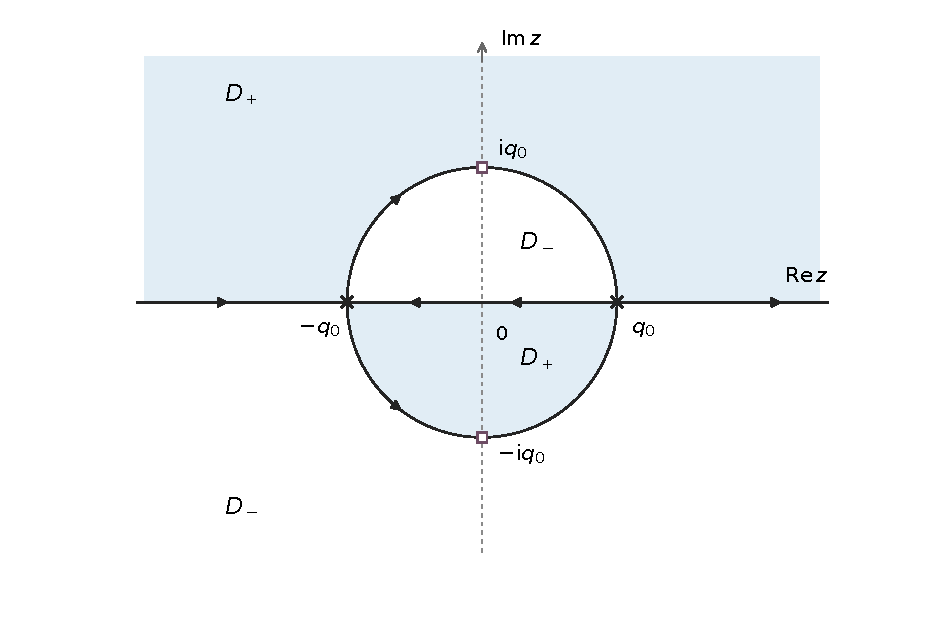
\includegraphics[width=0.78\textwidth]{figures/analytic-regions.pdf}
\caption{HMB 的单值化谱平面. 公共边界 $\Sigma$ 由实轴与圆 $|z|=q_0$ 组成; 淡蓝色区域为 $D_+$, 白色区域为 $D_-$. 箭头使 $D_+$ 位于定向边界的左侧. 方形点为分支点, 叉形点为边界交点.}
\label{fig:analytic-regions}
\end{figure}

为进行后续的轮廓积分, 将 $\Sigma$ 定向为 $D_+$ 位于左侧: 实轴外段朝右, 内段朝左, 上半圆顺时针, 下半圆逆时针. $z=\pm\ii q_0$ 为背景特征向量退化的分支点, $z=\pm q_0$ 为轮廓交点. 共振原像 $z_a^\pm$ 处空间谱问题正则; 其 Jost 值取固定 $t$ 的空间归一化.

\section{非零背景的直接散射}\label{ch:direct}

\subsection{空间归一化与 Volterra 方程}
固定 $t\in I$. 在 $\Sigma\mathbin{\backslash}\{0,\pm\ii q_0\}$ 上,
以空间端态定义 Jost 解 $\chi_\pm$:
\begin{equation}\label{eq:jost-normalization}
\chi_{\pm,x}=U\chi_\pm,\qquad
\chi_\pm(x,t,z)e^{\ii\lambda(z)x\sg}\longrightarrow Y(z),
\quad x\to\pm\infty.
\end{equation}
定义去除空间振荡后的矩阵
\begin{equation}\label{eq:modified-jost}
\mu_\pm=\chi_\pm e^{\ii\lambda x\sg},\qquad
\chi_\pm=\mu_\pm e^{-\ii\lambda x\sg},\qquad
\mu_\pm\longrightarrow Y.
\end{equation}
此定义包含两个共振原像, 不需要在共振处对完整传播指数求值.
记 $\Delta Q=Q-Q_\infty$. 下面先构造分支点以外的解析列.

\paragraph{空间指数的两列与求导.}
右乘 $e^{\ii\lambda x\sg}$ 分别给第一、二列乘 $e^{\ii\lambda x}$ 与 $e^{-\ii\lambda x}$, 因而
\[
\chi_{\pm,1}=e^{-\ii\lambda x}\mu_{\pm,1},\qquad
\chi_{\pm,2}=e^{\ii\lambda x}\mu_{\pm,2}.
\]
把 $\mu_\pm=\chi_\pm e^{\ii\lambda x\sg}$ 求导,
\[
(\mu_\pm)_x
=U\chi_\pm e^{\ii\lambda x\sg}
+\chi_\pm\ii\lambda\sg e^{\ii\lambda x\sg}
=U\mu_\pm+\ii\lambda\mu_\pm\sg.
\]
矩阵 $\sg$ 可以与对角指数交换, 但不能任意穿过 $\mu_\pm$.
这里没有时间指数; $t$ 是势函数的参数, 其演化在第 \ref{ch:scattering} 节另行研究.
\begin{theorem}[Jost 解与解析列]\label{thm:jost}
设光场满足基本条件中的空间要求. 对 $\Sigma$ 上除 $0,\pm\ii q_0$ 外的谱点, Volterra 方程
\begin{equation}\label{eq:volterra}
\mu_\pm(x,z)=Y(z)+\int_{\pm\infty}^{x}
Y(z)e^{-\ii\lambda(z)(x-y)\sg}Y(z)^{-1}
\Delta Q(y)\mu_\pm(y,z)e^{\ii\lambda(z)(x-y)\sg}\,\dd y
\end{equation}
有唯一关于 $x$ 有界的解. 列 $\mu_{-,1},\mu_{+,2}$ 在 $D_+$ 解析, 列 $\mu_{+,1},\mu_{-,2}$ 在 $D_-$ 解析, 并连续延拓到各自闭域中避开 $0,\pm\ii q_0$ 的紧集. $\chi_\pm=\mu_\pm e^{-\ii\lambda x\sg}$ 是满足 \eqref{eq:jost-normalization} 的唯一空间 Jost 解, 其中包含 $z=z_a^\pm$.
\end{theorem}
\begin{proof}
修正空间方程及其背景恒等式为
\[
(\mu_\pm)_x=U\mu_\pm+\ii\lambda\mu_\pm\sg,\qquad U_\infty Y=-\ii\lambda Y\sg.
\]

\par\medskip\noindent\textbf{把变分常数公式展开成积分因子的计算.}\quad
在当前的 $z$ 上, $Y$ 与 $x$ 无关且可逆. 把
$U=U_\infty+\Delta Q$ 代入上式, 再左乘 $Y^{-1}$, 得
\begin{align*}
(Y^{-1}\mu_\pm)_x
&=Y^{-1}U_\infty\mu_\pm
+Y^{-1}\Delta Q\mu_\pm
+\ii\lambda Y^{-1}\mu_\pm\sg\\
&=-\ii\lambda\sg Y^{-1}\mu_\pm
+\ii\lambda Y^{-1}\mu_\pm\sg
+Y^{-1}\Delta Q\mu_\pm.
\end{align*}
这里用到的背景恒等式在乘以 $Y^{-1}$ 以后为
\[
Y^{-1}U_\infty Y=-\ii\lambda\sg,
\qquad
Y^{-1}U_\infty=-\ii\lambda\sg Y^{-1}.
\]
现在左右同时乘积分因子. 对整个乘积求导:
\begin{align*}
&\partial_x\bigl(e^{\ii\lambda x\sg}Y^{-1}\mu_\pm
 e^{-\ii\lambda x\sg}\bigr)\\
&=\ii\lambda\sg e^{\ii\lambda x\sg}Y^{-1}\mu_\pm
 e^{-\ii\lambda x\sg}
+e^{\ii\lambda x\sg}(Y^{-1}\mu_\pm)_x
 e^{-\ii\lambda x\sg}\\
&\quad-e^{\ii\lambda x\sg}Y^{-1}\mu_\pm
 \ii\lambda\sg e^{-\ii\lambda x\sg}\\
&=e^{\ii\lambda x\sg}Y^{-1}\Delta Q(x)\mu_\pm(x)
 e^{-\ii\lambda x\sg}.
\end{align*}
第一行求导产生的左侧项, 恰好与微分方程中的
$-\ii\lambda\sg Y^{-1}\mu_\pm$ 相消;
右侧的两项也恰好相消. 从相应的归一化端积分到 $x$, 得
\begin{align*}
&e^{\ii\lambda x\sg}Y^{-1}\mu_\pm(x)e^{-\ii\lambda x\sg}\\
&=I+\int_{\pm\infty}^{x}
 e^{\ii\lambda y\sg}Y^{-1}\Delta Q(y)\mu_\pm(y)
 e^{-\ii\lambda y\sg}\,\dd y.
\end{align*}
再左乘 $Ye^{-\ii\lambda x\sg}$, 右乘
$e^{\ii\lambda x\sg}$, 得
\begin{align*}
\mu_\pm(x)
&=Y+\int_{\pm\infty}^{x}
 Ye^{-\ii\lambda(x-y)\sg}Y^{-1}
 \Delta Q(y)\mu_\pm(y)e^{\ii\lambda(x-y)\sg}\,\dd y.
\end{align*}
对 $+\infty$ 端, 积分方向应原样保留:
\[
\int_{+\infty}^{x}(\cdots)\,\dd y
=-\int_x^{+\infty}(\cdots)\,\dd y.
\]
这个负号在求导时与下限求导的负号抵消.
在连续谱上积分因子有界, 可以从端点归一化直接得到上式.
向非实谱延拓时应逐列使用下文的有界核, 而不是要求整个
$e^{\ii\lambda x\sg}$ 在无穷远有界.

对 $Y^{-1}\mu_\pm$ 使用变分常数公式, 得到 \eqref{eq:volterra}. 令 $s_1=1,s_2=-1$, 第 $j$ 列的传播核为
\begin{equation}\label{eq:columnkernel}
K_j(r,z)=e^{\ii s_j\lambda r}Y e^{-\ii\lambda r\sg}Y^{-1},\qquad r=x-y.
\end{equation}

\par\medskip\noindent\textbf{四种列核的指数从何而来.}\quad
在矩阵积分式中取第 $j$ 列, 最右边的对角矩阵只给该列乘
$e^{\ii s_j\lambda(x-y)}$. 因此有
\[
\mu_{\pm,j}(x)
=Y_j+\int_{\pm\infty}^{x}
K_j(x-y,z)\Delta Q(y)\mu_{\pm,j}(y)\,\dd y.
\]
把两个指数相乘, 第一列和第二列分别给出
\begin{align*}
K_1(r,z)
&=Y\begin{pmatrix}e^{\ii\lambda r}e^{-\ii\lambda r}&0\\
0&e^{\ii\lambda r}e^{\ii\lambda r}\end{pmatrix}Y^{-1}
=Y\begin{pmatrix}1&0\\0&e^{2\ii\lambda r}\end{pmatrix}Y^{-1},\\
K_2(r,z)
&=Y\begin{pmatrix}e^{-\ii\lambda r}e^{-\ii\lambda r}&0\\
0&e^{-\ii\lambda r}e^{\ii\lambda r}\end{pmatrix}Y^{-1}
=Y\begin{pmatrix}e^{-2\ii\lambda r}&0\\0&1\end{pmatrix}Y^{-1}.
\end{align*}
计算模时要同时看积分方向与谱根的虚部:
\[
|e^{2\ii\lambda r}|=e^{-2r\operatorname{Im}\lambda},
\qquad
|e^{-2\ii\lambda r}|=e^{2r\operatorname{Im}\lambda}.
\]
四种情况逐一为
\begin{align*}
\mu_{-,1}:&\quad y\le x,\ r\ge0,\ \operatorname{Im}\lambda\ge0,
& e^{-2r\operatorname{Im}\lambda}&\le1,\\
\mu_{+,2}:&\quad y\ge x,\ r\le0,\ \operatorname{Im}\lambda\ge0,
& e^{2r\operatorname{Im}\lambda}&\le1,\\
\mu_{+,1}:&\quad y\ge x,\ r\le0,\ \operatorname{Im}\lambda\le0,
& e^{-2r\operatorname{Im}\lambda}&\le1,\\
\mu_{-,2}:&\quad y\le x,\ r\ge0,\ \operatorname{Im}\lambda\le0,
& e^{2r\operatorname{Im}\lambda}&\le1.
\end{align*}
前两列属于 $D_+$, 后两列属于 $D_-$.
例如 $\mu_{+,1}$ 不能沿 $D_+$ 用同一个正端积分式构造,
因为这时 $r\le0$ 而 $\operatorname{Im}\lambda>0$,
$e^{-2r\operatorname{Im}\lambda}$ 在远端增长.
这正是必须区分列而不能给整个 Jost 矩阵指定一个解析域的原因.

以 $e_1,e_2$ 表示标准基向量. 对于负端第一列, 令 $w=Y^{-1}\mu_{-,1}$, 则
\begin{equation}\label{eq:jost-column-volterra}
w(x,z)=e_1+\int_{-\infty}^{x}G(x-y,z)\Delta Q(y)Y(z)w(y,z)\,\dd y,
\end{equation}
其中
\begin{equation}\label{eq:jost-Gkernel}
G(r,z)=\diag(1,e^{2\ii\lambda r})Y^{-1}
=\dfrac{1}{\gamma(z)}
\begin{pmatrix}
1&\dfrac{\ii q_0}{z}\\[4pt]
\dfrac{\ii q_0}{z}e^{2\ii\lambda r}&e^{2\ii\lambda r}
\end{pmatrix}.
\end{equation}
第一列对应的对角指数为 $\diag(1,e^{2\ii\lambda r})$, 第二列为 $\diag(e^{-2\ii\lambda r},1)$. 由 $r=x-y$, 四列的积分方向及指数模分别满足
\begin{align*}
\mu_{-,1}:&\quad y\le x,\ r\ge0,\ \operatorname{Im}\lambda\ge0,
& e^{-2r\operatorname{Im}\lambda}&\le1,\\
\mu_{+,2}:&\quad y\ge x,\ r\le0,\ \operatorname{Im}\lambda\ge0,
& e^{2r\operatorname{Im}\lambda}&\le1,\\
\mu_{+,1}:&\quad y\ge x,\ r\le0,\ \operatorname{Im}\lambda\le0,
& e^{-2r\operatorname{Im}\lambda}&\le1,\\
\mu_{-,2}:&\quad y\le x,\ r\ge0,\ \operatorname{Im}\lambda\le0,
& e^{2r\operatorname{Im}\lambda}&\le1.
\end{align*}
故前两列对应 $D_+$, 后两列对应 $D_-$.


\par\medskip\noindent\textbf{负端第一列的两个分量积分式.}\quad
$w=Y^{-1}\mu_{-,1}$ 沿用原文记号. 先把进入积分的矩阵乘法写全:
\[
\Delta Q(y)=\begin{pmatrix}0&q(y)-q_0\\
-\conj{q(y)}+q_0&0\end{pmatrix},
\qquad
Yw=\begin{pmatrix}
w_1-\dfrac{\ii q_0}{z}w_2\\
-\dfrac{\ii q_0}{z}w_1+w_2
\end{pmatrix}.
\]
因此
\[
\Delta Q(y)Yw
=\begin{pmatrix}
(q-q_0)\left(-\dfrac{\ii q_0}{z}w_1+w_2\right)\\
-(\conj{q}-q_0)\left(w_1-\dfrac{\ii q_0}{z}w_2\right)
\end{pmatrix}.
\]
在这里所有 $q,w$ 均取 $y$ 处的值. 再左乘 $G$, 得
\begin{align*}
w_1(x)
&=1+\dfrac{1}{\gamma}\int_{-\infty}^{x}
(q-q_0)\left(-\dfrac{\ii q_0}{z}w_1+w_2\right)\,\dd y\\
&\quad-\dfrac{\ii q_0}{z\gamma}\int_{-\infty}^{x}(\conj{q}-q_0)
\left(w_1-\dfrac{\ii q_0}{z}w_2\right)\,\dd y,\\
w_2(x)
&=\dfrac{\ii q_0}{z\gamma}\int_{-\infty}^{x}e^{2\ii\lambda(x-y)}(q-q_0)
\left(-\dfrac{\ii q_0}{z}w_1+w_2\right)\,\dd y\\
&\quad-\dfrac{1}{\gamma}\int_{-\infty}^{x}e^{2\ii\lambda(x-y)}
(\conj{q}-q_0)\left(w_1-\dfrac{\ii q_0}{z}w_2\right)\,\dd y.
\end{align*}
这两个式子显示: 背景列 $e_1$ 的第二分量为零,
而唯一可能增长的指数只出现在第二分量的传播中.
同样的矩阵乘法对第二列将指数置于第一行.

采用向量范数 $\|v\|_1=|v_1|+|v_2|$ 及其诱导矩阵范数. 由
\[
\|\Delta Q(y)\|_1=|q(y)-q_0|,\qquad
\|Y\|_1=1+\dfrac{q_0}{|z|},\qquad
\|Y^{-1}\|_1=\dfrac{1+\dfrac{q_0}{|z|}}{|\gamma(z)|},
\]
可得 HMB 积分核的具体估计
\begin{equation}\label{eq:jost-kernel-estimate}
\|G(x-y,z)\Delta Q(y)Y\|_1
\le c(z)|q(y)-q_0|,\qquad
c(z)=\dfrac{\left(1+\dfrac{q_0}{|z|}\right)^2}{\left|1+\dfrac{q_0^2}{z^2}\right|}.
\end{equation}
取 $K\subset\overline{D_+}\mathbin{\backslash}\{0,\pm\ii q_0\}$ 为紧集, 记
\[
c_{K}=\max\limits_{z\in K}c(z),\qquad
M_{K}(x)=c_{K}\int_{-\infty}^{x}|q(y)-q_0|\,\dd y.
\]

\par\medskip\noindent\textbf{矩阵范数估计中的每一个因子.}\quad
诱导 $1$ 范数是各列绝对值之和的最大值. 由上面三个矩阵的列和,
\begin{align*}
\|\Delta Q\|_1
&=\max\{|\conj{q}-q_0|,|q-q_0|\}=|q-q_0|,\\
\|Y\|_1
&=\max\left\{1+\dfrac{q_0}{|z|},1+\dfrac{q_0}{|z|}\right\}
=1+\dfrac{q_0}{|z|},\\
\|G(r,z)\|_1
&\le\dfrac{1}{|\gamma|}
\max\left\{1+\dfrac{q_0}{|z|},\dfrac{q_0}{|z|}+1\right\}
=\dfrac{1+\dfrac{q_0}{|z|}}{|\gamma|}.
\end{align*}
最后一行使用了允许方向上的 $|e^{2\ii\lambda r}|\le1$.
接着按乘法次序估计,
\begin{align*}
\|G\Delta QYw\|_1
&\le\|G\|_1\|\Delta Q\|_1\|Y\|_1\|w\|_1\\
&\le\dfrac{\left(1+\dfrac{q_0}{|z|}\right)^2}{|\gamma|}
|q-q_0|\|w\|_1.
\end{align*}
紧集避开 $z=0$ 与 $\gamma=0$ 的两点, 因而 $c_{ K}$ 有限.
$M_{ K}$ 是非减的绝对连续函数, 且几乎处处满足
\[
M_{ K}'(x)=c_{ K}|q(x)-q_0|,
\qquad M_{ K}(-\infty)=0.
\]
这一个导数等式正是下文阶乘分母的来源.

构造 Neumann 级数
\begin{equation}\label{eq:jost-neumann}
\begin{aligned}
w&=\sum\limits_{n=0}^{\infty}w^{(n)},\qquad w^{(0)}=e_1,\\
w^{(n+1)}&=\int_{-\infty}^{x}G(x-y,z)\Delta Q(y)Yw^{(n)}(y,z)\,\dd y.
\end{aligned}
\end{equation}
若 $\|w^{(n)}(y,z)\|_1\le \dfrac{M_{K}(y)^n}{n!}$, 则
\[
\|w^{(n+1)}(x,z)\|_1\le\dfrac{1}{n!}\int_{-\infty}^{x}c_{K}|q(y)-q_0|M_{K}(y)^n\,\dd y
=\dfrac{M_{K}(x)^{n+1}}{(n+1)!}.
\]
归纳即得
\begin{equation}\label{eq:jost-factorial}
\|w^{(n)}(x,z)\|_1\le\dfrac{M_{K}(x)^n}{n!},\qquad
\|w(x,z)-e_1\|_1\le e^{M_{K}(x)}-1.
\end{equation}

\par\medskip\noindent\textbf{把逐次积分真正展开到阶乘.}\quad
第一次与第二次迭代分别满足
\begin{align*}
\|w^{(1)}(x,z)\|_1
&\le\int_{-\infty}^{x}M_{ K}'(y)\,\dd y
=M_{ K}(x),\\
\|w^{(2)}(x,z)\|_1
&\le\int_{-\infty}^{x}M_{ K}'(y)
\int_{-\infty}^{y}M_{ K}'(y_1)\,\dd y_1\,\dd y\\
&=\int_{-\infty}^{x}M_{ K}'(y)M_{ K}(y)\,\dd y
=\dfrac{M_{ K}(x)^2}{2}.
\end{align*}
第三次同样得到
\[
\|w^{(3)}(x,z)\|_1
\le\int_{-\infty}^{x}M_{ K}'(y)
\dfrac{M_{ K}(y)^2}{2}\,\dd y
=\dfrac{M_{ K}(x)^3}{6}.
\]
一般一步的等号由微积分基本定理逐行给出:
\begin{align*}
\dfrac{1}{n!}\int_{-\infty}^{x}
M_{ K}'(y)M_{ K}(y)^n\,\dd y
&=\dfrac{1}{n!}\int_{-\infty}^{x}
\dfrac{1}{n+1}\partial_y\bigl(M_{ K}(y)^{n+1}\bigr)\,\dd y\\
&=\dfrac{M_{ K}(x)^{n+1}-M_{ K}(-\infty)^{n+1}}{(n+1)!}\\
&=\dfrac{M_{ K}(x)^{n+1}}{(n+1)!}.
\end{align*}
等价地, 第 $n$ 次迭代的积分区域是
\[
-\infty<y_n<y_{n-1}<\cdots<y_1<x.
\]
把 $( -\infty,x)^n$ 按 $n$ 个坐标的先后次序分成 $n!$ 个区域;
被积的范数上界是各坐标中同一非负函数的乘积, 因而每个区域的积分相等.
于是其积分为整个乘积积分的 $\dfrac{1}{n!}$, 即
$\dfrac{M_{ K}(x)^n}{n!}$.
求和时从 $n=1$ 开始的部分为
\[
\sum\limits_{n=1}^{\infty}\dfrac{M_{ K}(x)^n}{n!}
=e^{M_{ K}(x)}-1.
\]
特别地, 不要求 $\|q-q_0\|_{L^1}$ 小于某个数;
阶乘使任意有限的 $L^1$ 质量都能给出收敛.

由于 $M_{K}(x)\le c_{K}\|q-q_0\|_{L^1}$, 级数对实 $x$ 及 $z\in K$ 绝对一致收敛, 且在 $x\to-\infty$ 时趋于 $e_1$. 每一迭代项在 $D_+$ 解析, 并在相应闭域上连续; 上述一致估计保证其和 $w$ 及 $\mu_{-,1}=Yw$ 也具有这些性质.


\par\medskip\noindent\textbf{参数解析性与闭域连续性所用的控制.}\quad
对任一固定有限的 $x$, 先把积分在 $y=-R$ 处截断.
在有限区间上, 核的各矩阵元都是 $z$ 的解析函数,
因为 $Y,Y^{-1},\lambda$ 在当前紧集附近解析, 指数是整函数.
再让 $R\to+\infty$, 积分尾部的范数至多为
\[
c_{ K}\sup\limits_{y,z}\|w^{(n)}(y,z)\|_1
\int_{-\infty}^{-R}|q(y)-q_0|\,\dd y,
\]
它与 $z\in K$ 无关并趋于零.
所以每一项 $w^{(n)}$ 都是解析函数的一致极限.
对所有迭代项再使用
\[
\sum\limits_{n=0}^{\infty}
\sup\limits_{x\in\mathbb R,z\in K}\|w^{(n)}(x,z)\|_1
\le\sum\limits_{n=0}^{\infty}
\dfrac{\bigl(c_{ K}\|q-q_0\|_{L^1}\bigr)^n}{n!}<\infty.
\]
解析函数列的紧集一致极限仍然解析.
若 $z$ 从解析域趋向闭域边界, 核逐点连续,
上面同一个可积上界仍适用; 对每项与级数分别取极限,
即可交换边界极限、积分和无穷求和.
这里不声称仅靠 $L^1$ 就能在边界上任意次求 $z$ 导数;
对导数直接估计会出现 $|x-y|$, 需要与所求结论相适应的矩条件.

对两个有界解之差 $d$ 迭代 $n$ 次, 有
\[
\|d(x,z)\|_1\le\|d(\cdot,z)\|_{L^\infty}\dfrac{M_{K}(x)^n}{n!}\longrightarrow0,
\]
从而解唯一. 其余三列同理.

\par\medskip\noindent\textbf{唯一性与空间微分各自怎样完成.}\quad
差 $d$ 的自由项为零. 第一次应用积分方程给出
\[
\|d(x,z)\|_1\le\|d\|_{L^\infty}M_{ K}(x).
\]
把同一个积分式再次代入积分中的 $d(y,z)$,
积分区域成为 $y_1\le x,y_2\le y_1$, 故
\[
\|d(x,z)\|_1\le\|d\|_{L^\infty}
\dfrac{M_{ K}(x)^2}{2!}.
\]
重复 $n$ 次后就是原文所列估计. 对固定 $M_{ K}(x)$,
相邻上界之比为 $\dfrac{M_{ K}(x)}{n+1}$, 趋于零,
因此右端趋于零, 从而 $d(x,z)=0$.
对空间导数, 直接使用原文的列核有
\[
K_j(0,z)=I,
\qquad
\partial_rK_j(r,z)=(U_\infty+\ii s_j\lambda I)K_j(r,z).
\]
这是因为 $Ye^{-\ii\lambda r\sg}Y^{-1}=e^{rU_\infty}$.
逐列对积分式求导, 可得
\begin{align*}
(\mu_{\pm,j})_x
&=\Delta Q(x)\mu_{\pm,j}(x)
+\int_{\pm\infty}^{x}(U_\infty+\ii s_j\lambda I)
 K_j(x-y,z)\Delta Q(y)\mu_{\pm,j}(y)\,\dd y\\
&=\Delta Q\mu_{\pm,j}
+(U_\infty+\ii s_j\lambda I)(\mu_{\pm,j}-Y_j)\\
&=(U+\ii s_j\lambda I)\mu_{\pm,j}.
\end{align*}
最后使用 $(U_\infty+\ii s_j\lambda I)Y_j=0$.
故两列合起来满足修正空间方程.
再计算恢复指数后的导数:
\begin{align*}
\partial_x(\mu_{\pm,j}e^{\ii s_j(-\lambda x)})
&=(U\mu_{\pm,j}+\ii s_j\lambda\mu_{\pm,j})e^{\ii s_j(-\lambda x)}
-\ii s_j\lambda\mu_{\pm,j}e^{\ii s_j(-\lambda x)}\\
&=U\chi_{\pm,j}.
\end{align*}
在目前的低正则性假设下, 上述空间导数理解为几乎处处导数,
解在有限区间上绝对连续; 若 $q$ 连续, 等式处处成立.
\end{proof}

\subsection{分支点的连续延拓}
\begin{lemma}[分支点的空间极限]\label{prop:jost-branch}
基本条件给出加权可积性
\begin{equation}\label{eq:jost-weighted}
\int_{-\infty}^{+\infty}(1+|x|)|q(x)-q_0|\,\dd x<\infty.
\end{equation}
在此条件下, 每个 Jost 解析列均可从其闭解析域连续延拓到分支点 $z_b=\pm\ii q_0$. 端点值满足
\begin{equation}\label{eq:jost-branch-volterra}
\mu_\pm(x,z_b)=Y(z_b)+\int_{\pm\infty}^{x}
[I+(x-y)U_\infty(z_b)]\Delta Q(y)\mu_\pm(y,z_b)\,\dd y,
\end{equation}
并在对应归一化端趋于 $Y(z_b)$, 满足空间谱方程, 且秩为一.
\end{lemma}
\begin{proof}

\par\medskip\noindent\textbf{为什么分支点必须重新估计核.}\quad
当 $z\to z_b$, $\gamma(z)\to0$, 因而前面的
$c(z)$ 发散. 这只说明将 $Y$ 与 $Y^{-1}$ 分开估计过粗,
并不说明二者夹住指数后的整体发散.
先把背景矩阵的平方完整相乘:
\[
\begin{pmatrix}-\ii k&q_0\\-q_0&\ii k\end{pmatrix}^2
=\begin{pmatrix}
-k^2-q_0^2&-\ii kq_0+\ii kq_0\\
\ii kq_0-\ii kq_0&-q_0^2-k^2
\end{pmatrix}
=-\lambda^2I.
\]
所以偶数次幂与奇数次幂分别为
\[
U_\infty^{2n}=(-1)^n\lambda^{2n}I,
\qquad
U_\infty^{2n+1}=(-1)^n\lambda^{2n}U_\infty.
\]
代入矩阵指数的幂级数并把偶奇两部分分开,
\begin{align*}
e^{rU_\infty}
&=\sum\limits_{n=0}^{\infty}\dfrac{(-1)^n(\lambda r)^{2n}}{(2n)!}I
+\sum\limits_{n=0}^{\infty}\dfrac{(-1)^n\lambda^{2n}r^{2n+1}}{(2n+1)!}U_\infty\\
&=\cos(\lambda r)I+\dfrac{\sin(\lambda r)}{\lambda}U_\infty.
\end{align*}
在 $\lambda=0$ 处第二个系数按连续值取 $r$.

由 $U_\infty^2=-\lambda^2I$, 背景传播矩阵可写为
\begin{equation}\label{eq:background-propagator}
e^{rU_\infty}
=\cos(\lambda r)I+\dfrac{\sin(\lambda r)}{\lambda}U_\infty
\longrightarrow I+rU_\infty(z_b),\qquad z\to z_b.
\end{equation}
将 \eqref{eq:columnkernel} 写为
\begin{equation}\label{eq:branch-columnkernel}
K_j(r,z)=\dfrac{1+e^{2\ii s_j\lambda r}}{2}I
+\dfrac{e^{2\ii s_j\lambda r}-1}{2\ii s_j\lambda}U_\infty(z).
\end{equation}

\par\medskip\noindent\textbf{消掉分支点的表面分母.}\quad
将上式乘上列核中的 $e^{\ii s_j\lambda r}$.
利用 $s_j=\pm1$, 分别计算
\begin{align*}
e^{\ii s_j\lambda r}\cos(\lambda r)
&=\dfrac{1+e^{2\ii s_j\lambda r}}{2},\\
e^{\ii s_j\lambda r}\dfrac{\sin(\lambda r)}{\lambda}
&=\dfrac{e^{2\ii s_j\lambda r}-1}{2\ii s_j\lambda}.
\end{align*}
这得到原文的列核表达式. 第二个系数不是实质的极点:
\begin{align*}
e^{2\ii s_j\lambda r}-1
&=\int_0^1\partial_\tau
 e^{2\ii s_j\tau\lambda r}\,\dd\tau\\
&=2\ii s_j\lambda r\int_0^1
 e^{2\ii s_j\tau\lambda r}\,\dd\tau.
\end{align*}
当 $\lambda\to0$ 时, 这个积分趋于 1, 因而商趋于 $r$.
如果 $s_j\operatorname{Im}\lambda\,r\ge0$, 则每个
$0\le\tau\le1$ 上的指数模均不超过 1, 于是
\[
\left|\dfrac{1+e^{2\ii s_j\lambda r}}{2}\right|\le1,
\qquad
\left|\dfrac{e^{2\ii s_j\lambda r}-1}{2\ii s_j\lambda}\right|
\le|r|.
\]
故只需控制 $U_\infty$ 在分支点邻域的范数,
就能得到 $1+C_b|r|$ 的一致上界.
这解释了一阶空间矩为何足以处理分支点.

在该列允许的积分方向及闭解析域内, $s_j\operatorname{Im}\lambda\,r\ge0$, 且
\[
\dfrac{e^{2\ii s_j\lambda r}-1}{2\ii s_j\lambda}
=r\int_0^1 e^{2\ii s_j\tau\lambda r}\,\dd\tau,\qquad
\|K_j(r,z)\|_1\le1+C_b|r|.
\]
其中 $C_b$ 在 $z_b$ 的一个闭邻域内一致有界, 且 $K_j(r,z_b)=I+rU_\infty(z_b)$.

以负端为例, 固定 $b\in\mathbb R$, 对 $y\le x\le b$ 有
\[
1+C_b|x-y|\le A_b(1+|y|),\qquad
L_b(x)=A_b\int_{-\infty}^{x}(1+|y|)|q(y)-q_0|\,\dd y.
\]

\par\medskip\noindent\textbf{加权估计与半直线归一化.}\quad
当 $y\le x\le b$ 时,
\[
0\le x-y\le b-y\le|b|+|y|,
\]
故
\[
1+C_b|x-y|
\le 1+C_b|b|+C_b|y|
\le (1+C_b|b|+C_b)(1+|y|).
\]
因而可以把 $A_b$ 选为括号中的常数或更大的常数.
这不是对整个实轴统一控制 $|x-y|$;
它是在任意固定半直线 $x\le b$ 上控制积分核.
对第 $n$ 次迭代应用与前面完全相同的有序积分,
每个 $\Delta Q$ 的范数与 $1+C_b|x-y|$ 相乘后,
都由 $A_b(1+|y|)|q(y)-q_0|$ 控制.
于是阶乘估计的积分函数变为 $L_b$, 不再出现 $\dfrac{1}{\gamma}$.
又有
\[
\|\mu_{-,j}(x,z)-Y_j(z)\|_1
\le\left(\sup\limits_z\|Y_j(z)\|_1\right)(e^{L_b(x)}-1).
\]
加权可积性给出 $L_b(x)\to0$ 当 $x\to-\infty$,
所以端点归一化与 $z\to z_b$ 极限可以兼容.
在正端, 对 $b\le x\le y$ 用
$y-x\le |y|+|b|$, 并把积分上界改为从 $x$ 到 $+\infty$,
其余每一步保持相同.

列积分方程的第 $n$ 次迭代满足
\[
\|\mu_{-,j}^{(n)}(x,z)\|_1
\le C_Y\dfrac{L_b(x)^n}{n!},\qquad x\le b,
\]
其中 $C_Y$ 为该邻域内 $\|Y_j(z)\|_1$ 的统一界. 加权条件保证级数一致收敛, 逐项取极限得到 \eqref{eq:jost-branch-volterra}; $L_b(x)\to0$ 给出负端归一化. 正端的反向积分同理, 对两解之差的迭代也给出端点唯一性.


\par\medskip\noindent\textbf{端点空间方程与秩一结论的具体计算.}\quad
在 $z_b=\ii q_0$ 处,
\[
Y(z_b)=\begin{pmatrix}1&-1\\-1&1\end{pmatrix},
\qquad Y_2(z_b)=-Y_1(z_b).
\]
在 $z_b=-\ii q_0$ 处,
\[
Y(z_b)=\begin{pmatrix}1&1\\1&1\end{pmatrix},
\qquad Y_2(z_b)=Y_1(z_b).
\]
这两种线性关系都能逐列代入同一个端点 Volterra 方程.
负号情形下, $\mu_{\pm,2}+\mu_{\pm,1}$ 的自由项为零;
正号情形下, $\mu_{\pm,2}-\mu_{\pm,1}$ 的自由项为零.
由该半直线上的唯一性, 相应组合恒为零.
求端点方程的空间导数时,
\begin{align*}
(\mu_\pm)_x
&=\Delta Q(x)\mu_\pm(x)
+U_\infty\int_{\pm\infty}^{x}
\Delta Q(y)\mu_\pm(y)\,\dd y,\\
U_\infty\mu_\pm(x)
&=U_\infty Y
+\int_{\pm\infty}^{x}
\bigl(U_\infty+(x-y)U_\infty^2\bigr)
\Delta Q(y)\mu_\pm(y)\,\dd y\\
&=U_\infty\int_{\pm\infty}^{x}\Delta Q(y)\mu_\pm(y)\,\dd y.
\end{align*}
因此 $(\mu_\pm)_x=(U_\infty+\Delta Q)\mu_\pm=U\mu_\pm$.
第一列在归一化端趋于上面非零的 $Y_1$.
若它在某个有限点为零, 一阶线性初值问题的唯一性会使它处处为零,
与非零端态矛盾. 所以两列始终相关且至少一列非零, 矩阵秩恰为一.

对 \eqref{eq:jost-branch-volterra} 求导得到 $(\mu_\pm)_x=U(z_b)\mu_\pm$. 由端点唯一性, $Y(z_b)$ 两列的线性关系传递给 $\mu_\pm(x,z_b)$. 归一化端值非零, 线性系统的非零解不能在有限点为零, 故其秩恒为一.
\end{proof}

共振原像 $z_a^\pm$ 不使空间积分核退化, 因而 $\mu_\pm$ 在此仍由 \eqref{eq:volterra} 正则取值. 修正时间方程及共振相容性见第 \ref{ch:scattering} 节.

\subsection{散射矩阵与解析系数}
记 $\Sigma^\circ=\Sigma\mathbin{\backslash}\{0,\pm\ii q_0\}$. 在 $\Sigma^\circ$ 上, 两组 Jost 解为同一空间谱方程的基本解矩阵, 因而存在与 $x$ 无关的散射矩阵
\begin{equation}\label{eq:Sdef}
\chi_+(x,t,z)=\chi_-(x,t,z)S(z,t),\qquad S(z,t)=(s_{jk}(z,t))_{j,k=1}^{2}.
\end{equation}

\paragraph{为什么两组基底只相差一个常矩阵.}
先在非分支点处讨论. 下面将证明 $\det\chi_-=\gamma\ne0$,
所以散射关系等价于 $S=\chi_-^{-1}\chi_+$.
对恒等式 $\chi_-^{-1}\chi_-=I$ 求导,
\[
(\chi_-^{-1})_x\chi_-+\chi_-^{-1}(\chi_-)_x=0,
\qquad
(\chi_-^{-1})_x=-\chi_-^{-1}U.
\]
于是
\begin{align*}
S_x
&=(\chi_-^{-1})_x\chi_++\chi_-^{-1}(\chi_+)_x\\
&=-\chi_-^{-1}U\chi_++\chi_-^{-1}U\chi_+=0.
\end{align*}
这里 $U$ 可以随 $x$ 变化; 只因两组矩阵满足同一个空间方程,
这两个包含 $U$ 的项才精确相消.
把右乘矩阵逐元写出,
\[
(\chi_{-,1},\chi_{-,2})
\begin{pmatrix}s_{11}&s_{12}\\s_{21}&s_{22}\end{pmatrix}
=\bigl(s_{11}\chi_{-,1}+s_{21}\chi_{-,2},
 s_{12}\chi_{-,1}+s_{22}\chi_{-,2}\bigr).
\]
注意第一列的两个系数是 $s_{11},s_{21}$,
而不是散射矩阵的第一行. 所有后续反射系数的符号都依赖这一约定.

以下省略散射系数的 $t$ 自变量; 本节只证明它们与 $x$ 无关. 其列关系为
\begin{equation}\label{eq:scattering-columns}
\chi_{+,1}=s_{11}\chi_{-,1}+s_{21}\chi_{-,2},\qquad
\chi_{+,2}=s_{12}\chi_{-,1}+s_{22}\chi_{-,2}.
\end{equation}

\begin{proposition}[散射矩阵与 Wronskian]\label{prop:scattering}
在定理 \ref{thm:jost} 的条件下,
\begin{equation}\label{eq:detjost}
\det\chi_\pm=\det\mu_\pm=\gamma(z),\qquad \det S=1.
\end{equation}
散射系数满足
\begin{align}
s_{11}&=\dfrac{\det(\chi_{+,1},\chi_{-,2})}{\gamma},&
s_{22}&=\dfrac{\det(\chi_{-,1},\chi_{+,2})}{\gamma},\label{eq:wronskian}\\
s_{21}&=\dfrac{\det(\chi_{-,1},\chi_{+,1})}{\gamma},&
s_{12}&=\dfrac{\det(\chi_{+,2},\chi_{-,2})}{\gamma}.\nonumber
\end{align}
其中 $s_{11}$ 在 $D_-$ 解析, $s_{22}$ 在 $D_+$ 解析, 并连续延拓到相应闭域中避开 $0,\pm\ii q_0$ 的紧集. $s_{12},s_{21}$ 在 $\Sigma^\circ$ 上连续; 在共振原像处使用空间归一化值.
\end{proposition}
\begin{proof}

\par\medskip\noindent\textbf{Abel 恒等式在这个二阶系统中的完整求导.}\quad
空间方程的四个分量是
\begin{align*}
(\chi_{11})_x&=-\ii k\chi_{11}+q\chi_{21},&
(\chi_{12})_x&=-\ii k\chi_{12}+q\chi_{22},\\
(\chi_{21})_x&=-\conj{q}\chi_{11}+\ii k\chi_{21},&
(\chi_{22})_x&=-\conj{q}\chi_{12}+\ii k\chi_{22}.
\end{align*}
这里 $\chi$ 可以逐次取 $\chi_+$ 或 $\chi_-$,
并未引入新的谱解. 对二阶行列式的两项分别求导:
\begin{align*}
\partial_x\det\chi
&=\partial_x(\chi_{11}\chi_{22}-\chi_{12}\chi_{21})\\
&=(-\ii k\chi_{11}+q\chi_{21})\chi_{22}
+\chi_{11}(-\conj{q}\chi_{12}+\ii k\chi_{22})\\
&\quad-(-\ii k\chi_{12}+q\chi_{22})\chi_{21}
-\chi_{12}(-\conj{q}\chi_{11}+\ii k\chi_{21})\\
&=-\ii k\chi_{11}\chi_{22}+\ii k\chi_{11}\chi_{22}
+\ii k\chi_{12}\chi_{21}-\ii k\chi_{12}\chi_{21}\\
&\quad+q\chi_{21}\chi_{22}-q\chi_{22}\chi_{21}
-\conj{q}\chi_{11}\chi_{12}+\conj{q}\chi_{12}\chi_{11}=0.
\end{align*}
每个矩阵元是标量, 所以最后两组也能交换次序而相消.
归一化端的行列式为
\begin{align*}
\det\chi_\pm
&=\det\mu_\pm\det e^{-\ii\lambda x\sg}
=\det\mu_\pm\,e^{-\ii\lambda x}e^{\ii\lambda x}
=\det\mu_\pm,\\
\lim\limits_{x\to\pm\infty}\det\mu_\pm
&=\det\begin{pmatrix}1&-\dfrac{\ii q_0}{z}\\
-\dfrac{\ii q_0}{z}&1\end{pmatrix}
=1-\left(-\dfrac{\ii q_0}{z}\right)^2
=1+\dfrac{q_0^2}{z^2}=\gamma.
\end{align*}
由于行列式不随 $x$ 变化, 它等于自己的端点极限.
对散射关系取行列式,
\[
\gamma=\gamma\det S,
\qquad \gamma\ne0,
\qquad \det S=1.
\]

由 $\tr U=0$, Abel 恒等式给出 $\partial_x\det\chi_\pm=0$. 在归一化端取极限, 并使用 $\det e^{-\ii\lambda x\sg}=1$, 得到 $\det\chi_\pm=\gamma$. 对 \eqref{eq:Sdef} 取行列式即得 $\det S=1$.
\par\medskip\noindent\textbf{四个 Wronskian 分别怎样消去另一项.}\quad
二列行列式对每列都是线性的, 且两列相同的行列式为零.
对第一条列关系, 两种取法为
\begin{align*}
\det(\chi_{+,1},\chi_{-,2})
&=s_{11}\det(\chi_{-,1},\chi_{-,2})
+s_{21}\det(\chi_{-,2},\chi_{-,2})\\
&=s_{11}\gamma+s_{21}\cdot0=s_{11}\gamma,\\
\det(\chi_{-,1},\chi_{+,1})
&=s_{11}\det(\chi_{-,1},\chi_{-,1})
+s_{21}\det(\chi_{-,1},\chi_{-,2})\\
&=s_{11}\cdot0+s_{21}\gamma=s_{21}\gamma.
\end{align*}
对第二条列关系, 应按下面的列次序取行列式:
\begin{align*}
\det(\chi_{-,1},\chi_{+,2})
&=s_{12}\det(\chi_{-,1},\chi_{-,1})
+s_{22}\det(\chi_{-,1},\chi_{-,2})\\
&=s_{22}\gamma,\\
\det(\chi_{+,2},\chi_{-,2})
&=s_{12}\det(\chi_{-,1},\chi_{-,2})
+s_{22}\det(\chi_{-,2},\chi_{-,2})\\
&=s_{12}\gamma.
\end{align*}
例如, 若把最后一个行列式的两列反过来,
会得到 $-s_{12}\gamma$, 因而不能随意交换列序.
除以 $\gamma$ 后恰好得到原文四个散射系数.

对第一条列关系分别与 $\chi_{-,2}$、$\chi_{-,1}$ 取行列式, 有
\[
\det(\chi_{+,1},\chi_{-,2})=s_{11}\gamma,\qquad
\det(\chi_{-,1},\chi_{+,1})=s_{21}\gamma.
\]
第二条列关系同理给出 $s_{12},s_{22}$, 即 \eqref{eq:wronskian}.
\par\medskip\noindent\textbf{把四个行列式中的指数也逐个抽出.}\quad
由第一列与第二列分别带 $e^{-\ii\lambda x}$ 与 $e^{\ii\lambda x}$,
\begin{align*}
\det(\chi_{+,1},\chi_{-,2})
&=e^{-\ii\lambda x}e^{\ii\lambda x}
\det(\mu_{+,1},\mu_{-,2})
=\det(\mu_{+,1},\mu_{-,2}),\\
\det(\chi_{-,1},\chi_{+,2})
&=e^{-\ii\lambda x}e^{\ii\lambda x}
\det(\mu_{-,1},\mu_{+,2})
=\det(\mu_{-,1},\mu_{+,2}),\\
\det(\chi_{-,1},\chi_{+,1})
&=e^{-2\ii\lambda x}\det(\mu_{-,1},\mu_{+,1}),\\
\det(\chi_{+,2},\chi_{-,2})
&=e^{2\ii\lambda x}\det(\mu_{+,2},\mu_{-,2}).
\end{align*}
因此四个系数也可写为
\begin{align*}
s_{11}&=\dfrac{(\mu_+)_{11}(\mu_-)_{22}
-(\mu_-)_{12}(\mu_+)_{21}}{\gamma},\\
s_{22}&=\dfrac{(\mu_-)_{11}(\mu_+)_{22}
-(\mu_+)_{12}(\mu_-)_{21}}{\gamma},\\
s_{21}&=\dfrac{e^{-2\ii\lambda x}}{\gamma}
\bigl((\mu_-)_{11}(\mu_+)_{21}
-(\mu_+)_{11}(\mu_-)_{21}\bigr),\\
s_{12}&=\dfrac{e^{2\ii\lambda x}}{\gamma}
\bigl((\mu_+)_{12}(\mu_-)_{22}
-(\mu_-)_{12}(\mu_+)_{22}\bigr).
\end{align*}
$s_{22}$ 的两列恰为 $\mu_{-,1},\mu_{+,2}$,
二者都在 $D_+$ 解析; $s_{11}$ 的两列恰为
$\mu_{+,1},\mu_{-,2}$, 二者都在 $D_-$ 解析.
$\gamma$ 在相应开域没有零点, 所以除法保留解析性.
另一方面, $s_{21}$ 与 $s_{12}$ 所用两列来自相反解析域,
这里只能在共同边界上取值, 不能由这两个式子直接宣称全域解析.

对透射系数, 两列的指数相消, 故
\[
s_{11}=\dfrac{\det(\mu_{+,1},\mu_{-,2})}{\gamma},\qquad
s_{22}=\dfrac{\det(\mu_{-,1},\mu_{+,2})}{\gamma}.
\]
两个分子分别由 $D_-$ 和 $D_+$ 的解析列组成, 且 $\gamma$ 的零点只位于分支点. 定理 \ref{thm:jost} 因而给出所述解析性与连续性. 对非对角元, 列指数只留下连续因子 $e^{\pm2\ii(-\lambda x)}$, 故它们在 $\Sigma^\circ$ 上连续.
\end{proof}

按照 $\chi_+=\chi_-S$ 的约定, 以下称 $s_{11},s_{22}$ 为透射系数. 在其非零的谱弧上定义反射系数
\begin{equation}\label{eq:reflection}
\rho(z)=\dfrac{s_{21}(z)}{s_{11}(z)},\qquad
\widetilde\rho(z)=\dfrac{s_{12}(z)}{s_{22}(z)}.
\end{equation}
由 $\det S=1$,
\begin{equation}\label{eq:scattering-determinant}
s_{11}s_{22}-s_{12}s_{21}=1,\qquad
s_{11}s_{22}(1-\rho\widetilde\rho)=1.
\end{equation}

\paragraph{反射系数与行列式约束的代数.}
由定义, 在分母不为零的谱弧上有
\[
s_{21}=\rho s_{11},\qquad s_{12}=\widetilde\rho s_{22}.
\]
将这两式原次序代入行列式,
\begin{align*}
s_{11}s_{22}-s_{12}s_{21}
&=s_{11}s_{22}-(\widetilde\rho s_{22})(\rho s_{11})\\
&=s_{11}s_{22}(1-\rho\widetilde\rho)=1.
\end{align*}
由于这里都是标量函数, 可以交换乘法次序.
这也说明 $1-\rho\widetilde\rho$ 不能在该谱弧上为零.
共轭约化之后, 实轴上会有
$\widetilde\rho=-\conj\rho$, 从而该因子变成
$1+|\rho|^2$; 这里先保留原有符号形式,
以免把只在实轴成立的等式用于圆谱的非实点.

后续矩阵 RHP 取普通连续谱上 $s_{11}s_{22}\ne0$ 的散射数据; 分支点的边界正则性另行列入 RHP 的条件.

\subsection{共轭与换叶约化}\label{ch:symmetry}
复共轭与换叶分别作用为
\begin{equation}\label{eq:symmetry-domains}
z\mapsto\conj{z}:D_\pm\longrightarrow D_\mp,\qquad
h:z\mapsto-\dfrac{q_0^2}{z}:D_\pm\longrightarrow D_\mp.
\end{equation}

\paragraph{两种映射怎样作用于区域.}
共轭不改变 $|z|$, 而把 $\operatorname{Im}z$ 变为其相反数,
所以区域定义中的乘积满足
\[
\operatorname{Im}(\conj{z})
\left(1-\dfrac{q_0^2}{|\conj{z}|^2}\right)
=-\operatorname{Im}z\left(1-\dfrac{q_0^2}{|z|^2}\right).
\]
换叶映射则满足
\[
h(z)=-\dfrac{q_0^2\conj{z}}{|z|^2},
\qquad
\operatorname{Im}h(z)=\dfrac{q_0^2}{|z|^2}\operatorname{Im}z,
\qquad
|h(z)|^2=\dfrac{q_0^4}{|z|^2}.
\]
代回同一个区域判别式,
\begin{align*}
\operatorname{Im}h(z)
\left(1-\dfrac{q_0^2}{|h(z)|^2}\right)
&=\dfrac{q_0^2}{|z|^2}\operatorname{Im}z
\left(1-\dfrac{|z|^2}{q_0^2}\right)\\
&=-\operatorname{Im}z\left(1-\dfrac{q_0^2}{|z|^2}\right).
\end{align*}
所以两种映射分别都交换 $D_+$ 与 $D_-$.
它们的对易性可直接计算:
\[
h(\conj{z})=-\dfrac{q_0^2}{\conj{z}}
=\conj{\left(-\dfrac{q_0^2}{z}\right)}=\conj{h(z)}.
\]
连续作用两次换叶还给出
\[
h(h(z))=-\dfrac{q_0^2}{-\dfrac{q_0^2}{z}}=z.
\]
这些关系决定离散谱轨道, 也决定哪些列的等式能够在相同解析域中比较.

二者对易, 其复合保持 $D_\pm$. 以下先在普通连续谱上比较 Jost 归一化, 再将相应列关系延拓到解析域.

\begin{proposition}[Jost 解的共轭与换叶约化]\label{prop:symmetry}
令
\[
\sigma_2=\begin{pmatrix}0&-\ii\\\ii&0\end{pmatrix},\qquad
C(z)=\dfrac{\ii z}{q_0}\sigma_1.
\]
在定理 \ref{thm:jost} 的条件下,
\begin{equation}\label{eq:conjugation}
\chi_\pm(z)=\sigma_2\conj{\chi_\pm(\conj{z})}\sigma_2,\qquad
\mu_\pm(z)=\sigma_2\conj{\mu_\pm(\conj{z})}\sigma_2,
\end{equation}
\begin{equation}\label{eq:musheet}
\chi_\pm(h(z))=\chi_\pm(z)C(z),\qquad
\mu_\pm(h(z))=\mu_\pm(z)C(z).
\end{equation}
逐列写为
\begin{alignat}{2}
&\chi_{\pm,1}(z)=\ii\sigma_2\conj{\chi_{\pm,2}(\conj{z})},&\qquad
&\chi_{\pm,2}(z)=-\ii\sigma_2\conj{\chi_{\pm,1}(\conj{z})},\label{eq:jost-conjugate-columns}\\
&\chi_{\pm,1}(h(z))=\dfrac{\ii z}{q_0}\chi_{\pm,2}(z),&\qquad
&\chi_{\pm,2}(h(z))=\dfrac{\ii z}{q_0}\chi_{\pm,1}(z).\label{eq:jost-sheet-columns}
\end{alignat}
修正列 $\mu_{\pm,j}$ 满足相同关系.
\end{proposition}
\begin{proof}

\par\medskip\noindent\textbf{共轭约化中的矩阵乘法.}\quad
先计算三个常矩阵的基本关系:
\[
\sigma_2^2
=\begin{pmatrix}(-\ii)\ii&0\\0&\ii(-\ii)\end{pmatrix}=I,
\qquad
\sigma_2\sg
=\begin{pmatrix}0&\ii\\\ii&0\end{pmatrix},
\]
\[
\sigma_2\sg\sigma_2
=\begin{pmatrix}-1&0\\0&1\end{pmatrix}=-\sg,
\qquad
\sigma_2\sigma_1\sigma_2=-\sigma_1.
\]
对势矩阵则有
\begin{align*}
\sigma_2\conj{Q}
&=\begin{pmatrix}0&-\ii\\\ii&0\end{pmatrix}
\begin{pmatrix}0&\conj{q}\\-q&0\end{pmatrix}
=\begin{pmatrix}\ii q&0\\0&\ii\conj{q}\end{pmatrix},\\
\sigma_2\conj{Q}\sigma_2
&=\begin{pmatrix}0&q\\-\conj{q}&0\end{pmatrix}=Q.
\end{align*}
单值化有理函数的系数为实数, 所以
\[
\conj{k(\conj{z})}=k(z),
\qquad
\conj{\lambda(\conj{z})}=\lambda(z),
\qquad
\conj{F(k(\conj{z}))}=F(k(z)).
\]
于是
\begin{align*}
\sigma_2\conj{U(\conj{z})}\sigma_2
&=\sigma_2(\ii k(z)\sg+\conj{Q})\sigma_2\\
&=-\ii k(z)\sg+Q=U(z),\\
\sigma_2\conj{Y(\conj{z})}\sigma_2
&=\sigma_2\left(I+\dfrac{\ii q_0}{z}\sigma_1\right)\sigma_2\\
&=I-\dfrac{\ii q_0}{z}\sigma_1=Y(z).
\end{align*}
相位满足
\[
\conj{(-\lambda(\conj{z})x)}
=-\conj{\lambda(\conj{z})}
\bigl[x-\conj{F(k(\conj{z}))}t\bigr]
=-\lambda(z)[x-F(k(z))t]=(-\lambda(z)x).
\]
这里 $x,t$ 为实变量, 这一点在取共轭时也被使用了.

由 $\sigma_2\sg\sigma_2=-\sg$、$\sigma_2\conj{Q}\sigma_2=Q$ 及 $k(\conj{z})=\conj{k(z)}$,
\[
U(z)=\sigma_2\conj{U(\conj{z})}\sigma_2,\qquad
Y(z)=\sigma_2\conj{Y(\conj{z})}\sigma_2.
\]
又有 $\lambda(\conj{z})=\conj{\lambda(z)}$, 故
\[
\sigma_2\conj{Y(\conj{z})e^{-\ii\lambda(\conj{z})x\sg}}\sigma_2
=Y(z)e^{-\ii\lambda(z)x\sg}.
\]

\par\medskip\noindent\textbf{共轭指数的负号与列交换的负号.}\quad
取共轭先将 $\ii$ 变为 $-\ii$, 故
\[
\conj{e^{-\ii\lambda(\conj{z})x\sg}}
=e^{\ii\lambda(z)x\sg}.
\]
再与 $\sigma_2$ 共轭, 对角元交换:
\begin{align*}
\sigma_2 e^{\ii\lambda x\sg}\sigma_2
&=\sigma_2\begin{pmatrix}e^{\ii\lambda x}&0\\0&e^{-\ii\lambda x}\end{pmatrix}\sigma_2\\
&=\begin{pmatrix}e^{-\ii\lambda x}&0\\0&e^{\ii\lambda x}\end{pmatrix}
=e^{-\ii\lambda x\sg}.
\end{align*}
因为 $\sigma_2^2=I$, 乘积的约化可在中间插入 $I$:
\begin{align*}
\sigma_2\conj{Y(\conj{z})e^{-\ii\lambda(\conj{z})x\sg}}\sigma_2
&=(\sigma_2\conj{Y(\conj{z})}\sigma_2)
(\sigma_2 e^{\ii\lambda(z)x\sg}\sigma_2)\\
&=Y(z)e^{-\ii\lambda(z)x\sg}.
\end{align*}
对变换后的解求导,
\begin{align*}
\partial_x\bigl(\sigma_2\conj{\chi_\pm(\conj{z})}\sigma_2\bigr)
&=\sigma_2\conj{U(\conj{z})}\conj{\chi_\pm(\conj{z})}\sigma_2\\
&=U(z)\sigma_2\conj{\chi_\pm(\conj{z})}\sigma_2.
\end{align*}
这就是同一空间方程; 上式又给出同一端态,
所以可应用 Jost 唯一性.

共轭后的 Jost 解满足同一空间方程和同一归一化, 定理 \ref{thm:jost} 的唯一性给出 \eqref{eq:conjugation}.


\par\medskip\noindent\textbf{时间矩阵约化中有理项的核对.}\quad
对介质矩阵逐元计算,
\begin{align*}
\sigma_2\conj{R}\sigma_2
&=\sigma_2
\begin{pmatrix}\eta&-\conj{p}\\-p&-\eta\end{pmatrix}\sigma_2\\
&=\begin{pmatrix}-\eta&p\\\conj{p}&\eta\end{pmatrix}=-R.
\end{align*}
因此有理项经过约化时出现两个负号:
\[
\sigma_2\conj{\left(\dfrac{\ii R}{k(\conj{z})-a}\right)}\sigma_2
=-\dfrac{\ii\sigma_2\conj{R}\sigma_2}{k(z)-a}
=\dfrac{\ii R}{k(z)-a}.
\]
$\dfrac{\ii\Omega}{2}\sg$ 也由
$\conj{\ii}=-\ii$ 与 $\sigma_2\sg\sigma_2=-\sg$
的两个负号保持不变.
对多项式部分, 每个 $V_j$ 都是迹零矩阵,
其对角元纯虚且 $(V_j)_{21}=-\conj{(V_j)_{12}}$.
直接使用一般二阶乘法即有
\[
\sigma_2\conj{V_j}\sigma_2
=\begin{pmatrix}
\conj{(V_j)_{22}}&-\conj{(V_j)_{21}}\\
-\conj{(V_j)_{12}}&\conj{(V_j)_{11}}
\end{pmatrix}=V_j.
\]
例如 $q\conj{q_x}-q_x\conj{q}$ 的共轭是其相反数,
所以 $V_0$ 的对角元也确实纯虚.
这就逐项给出了 $V$ 的共轭约化.

换叶保持 $k$ 而使 $\lambda$ 变号. 直接由 \eqref{eq:E} 计算,
\begin{equation}\label{eq:Esheet}
Y(h(z))=I+\dfrac{\ii z}{q_0}\sigma_1=Y(z)C(z),\qquad
C(z)\sg=-\sg C(z).
\end{equation}

\par\medskip\noindent\textbf{换叶所需的全部代数恒等式.}\quad
把 $h(z)$ 代入 $k,\lambda$ 的有理表达式,
\begin{align*}
k(h(z))
&=\dfrac{1}{2}\left(-\dfrac{q_0^2}{z}
-\dfrac{q_0^2}{-\dfrac{q_0^2}{z}}\right)
=\dfrac{1}{2}\left(z-\dfrac{q_0^2}{z}\right)=k(z),\\
\lambda(h(z))
&=\dfrac{1}{2}\left(-\dfrac{q_0^2}{z}
+\dfrac{q_0^2}{-\dfrac{q_0^2}{z}}\right)
=-\dfrac{1}{2}\left(z+\dfrac{q_0^2}{z}\right)=-\lambda(z).
\end{align*}
因为 $F$ 只依赖 $k$, 可得 $F(k(h(z)))=F(k(z))$,
故 $(-\lambda(h(z))x)=-(-\lambda(z)x)$.
$Y$ 与 $C$ 的乘法也可直接展开:
\begin{align*}
Y(z)C(z)
&=\left(I-\dfrac{\ii q_0}{z}\sigma_1\right)
\dfrac{\ii z}{q_0}\sigma_1\\
&=\dfrac{\ii z}{q_0}\sigma_1
-\dfrac{\ii q_0}{z}\dfrac{\ii z}{q_0}\sigma_1^2\\
&=I+\dfrac{\ii z}{q_0}\sigma_1=Y(h(z)).
\end{align*}
其逆与两次换叶的一致性分别为
\[
C(z)^{-1}=-\dfrac{\ii q_0}{z}\sigma_1,
\qquad C(z)C(h(z))=I.
\]
由于
\[
\sigma_1\sg=\begin{pmatrix}0&-1\\1&0\end{pmatrix},
\qquad
\sg\sigma_1=\begin{pmatrix}0&1\\-1&0\end{pmatrix},
\]
有 $C\sg=-\sg C$.
把指数写为对角矩阵可逐元确认
\[
e^{-\ii\lambda x\sg}C
=C e^{\ii\lambda x\sg},
\qquad
C e^{-\ii\lambda x\sg}=e^{\ii\lambda x\sg}C.
\]
因此换叶不是简单地把指数换号后保持列号;
右乘 $C$ 同时交换了两列.

于是 $\chi_\pm(z)C(z)$ 在 $h(z)$ 处满足同一空间方程, 且
\[
Y(z)e^{-\ii\lambda(z)x\sg}C(z)
=Y(h(z))e^{-\ii\lambda(h(z))x\sg}.
\]
再次由唯一性得到 $\chi_\pm$ 的换叶关系. 去除指数时使用

\[
C(z)e^{-\ii\lambda(z)x\sg}=e^{\ii\lambda(z)x\sg}C(z)
\]
,
便得到 $\mu_\pm$ 的关系.
\par\medskip\noindent\textbf{修正 Jost 关系及四条列关系逐项展开.}\quad
从 $\chi(h(z))=\chi(z)C(z)$ 出发,
\begin{align*}
\mu(h(z))
&=\chi(h(z))e^{\ii\lambda(h(z))x\sg}\\
&=\chi(z)C(z)e^{-\ii\lambda(z)x\sg}\\
&=\chi(z)e^{\ii\lambda(z)x\sg}C(z)=\mu(z)C(z).
\end{align*}
共轭关系对 $\mu$ 的证明也保留两个指数负号:
\begin{align*}
\sigma_2\conj{\mu(\conj{z})}\sigma_2
&=\sigma_2\conj{\chi(\conj{z})}
 e^{-\ii\lambda(z)x\sg}\sigma_2\\
&=(\sigma_2\conj{\chi(\conj{z})}\sigma_2)
 (\sigma_2 e^{-\ii\lambda(z)x\sg}\sigma_2)\\
&=\chi(z)e^{\ii\lambda(z)x\sg}=\mu(z).
\end{align*}
把右乘 $\sigma_2$ 的结果写成两列,
\[
\conj{\chi(\conj{z})}\sigma_2
=\bigl(\ii\conj{\chi_2(\conj{z})},
-\ii\conj{\chi_1(\conj{z})}\bigr).
\]
再左乘 $\sigma_2$, 得
\[
\chi_1(z)=\ii\sigma_2\conj{\chi_2(\conj{z})},
\qquad
\chi_2(z)=-\ii\sigma_2\conj{\chi_1(\conj{z})}.
\]
右乘 $C$ 则没有两个不同的符号:
\[
(\chi_1,\chi_2)C
=\left(\dfrac{\ii z}{q_0}\chi_2,
\dfrac{\ii z}{q_0}\chi_1\right).
\]
相同乘法适用于 $\mu$.
对解析列比较时, 例如
$\mu_{-,1}(z)$ 与 $\mu_{-,2}(\conj{z})$,
右边的第二列在 $D_-$ 解析, 而共轭后的自变量属于 $D_+$;
所以两边确实在同一个区域上有意义.

右乘矩阵的两列分别给出 \eqref{eq:jost-conjugate-columns}--\eqref{eq:jost-sheet-columns}. 变换后的列具有 \eqref{eq:symmetry-domains} 所确定的解析域, 因此同一 Volterra 唯一性论证在各解析域内成立.
\end{proof}

\begin{proposition}[散射矩阵与反射数据的约化]\label{prop:scattering-symmetry}
散射矩阵满足
\begin{equation}\label{eq:scattering-symmetry}
S(z)=\sigma_2\conj{S(\conj{z})}\sigma_2,\qquad
S(h(z))=\sigma_1S(z)\sigma_1.
\end{equation}
特别地,
\begin{equation}\label{eq:sconj}
s_{22}(z)=\conj{s_{11}(\conj{z})},\qquad
s_{12}(z)=-\conj{s_{21}(\conj{z})},
\end{equation}
\begin{equation}\label{eq:ssheet}
s_{22}(h(z))=s_{11}(z),\qquad s_{12}(h(z))=s_{21}(z),
\end{equation}
\begin{equation}\label{eq:reflection-symmetry}
\rho(z)=-\conj{\widetilde\rho(\conj{z})},\qquad
\rho(h(z))=\widetilde\rho(z).
\end{equation}
透射系数的关系在相应解析域内成立. 在实谱的普通点,
\begin{equation}\label{eq:scattering-unitarity}
S(z)^\dagger S(z)=I,\qquad
|s_{11}(z)|^2+|s_{21}(z)|^2=1.
\end{equation}
\end{proposition}
\begin{proof}

\par\medskip\noindent\textbf{由基底的约化得到散射矩阵的约化.}\quad
先在 $\conj{z}$ 处写散射关系并取共轭,
\[
\conj{\chi_+(\conj{z})}
=\conj{\chi_-(\conj{z})}\conj{S(\conj{z})}.
\]
左右乘 $\sigma_2$, 并在乘积中间插入
$\sigma_2^2=I$, 得
\begin{align*}
\chi_+(z)
&=(\sigma_2\conj{\chi_-(\conj{z})}\sigma_2)
(\sigma_2\conj{S(\conj{z})}\sigma_2)\\
&=\chi_-(z)(\sigma_2\conj{S(\conj{z})}\sigma_2).
\end{align*}
与 $\chi_+=\chi_-S$ 比较, 左乘可逆的 $\chi_-^{-1}$,
得到共轭约化.
换叶时在 $h(z)$ 处写散射关系,
\[
\chi_+(z)C(z)=\chi_-(z)C(z)S(h(z)).
\]
同时原关系右乘 $C(z)$ 给出
$\chi_+(z)C(z)=\chi_-(z)S(z)C(z)$.
两式消去 $\chi_-$ 后,
\[
C(z)S(h(z))=S(z)C(z),
\qquad
S(h(z))=C(z)^{-1}S(z)C(z).
\]
$C$ 中非零的标量因子在共轭中抵消, 因而只留下
$\sigma_1S\sigma_1$.

将 \eqref{eq:conjugation} 代入 $\chi_+=\chi_-S$, 并利用 $\chi_-$ 的可逆性, 得到 \eqref{eq:scattering-symmetry} 的第一式. 比较
\[
\chi_+(z)C(z)=\chi_-(z)S(z)C(z)
=\chi_-(z)C(z)S(h(z)),
\]
得到
\[
S(h(z))=C(z)^{-1}S(z)C(z)=\sigma_1S(z)\sigma_1.
\]

\par\medskip\noindent\textbf{把两个矩阵约化完全展开为四个矩阵元.}\quad
共轭约化的右侧实际为
\begin{align*}
\sigma_2\conj{S(\conj{z})}\sigma_2
&=\begin{pmatrix}
\conj{s_{22}(\conj{z})}&-\conj{s_{21}(\conj{z})}\\
-\conj{s_{12}(\conj{z})}&\conj{s_{11}(\conj{z})}
\end{pmatrix}.
\end{align*}
故除了原文列出的两式之外, 另外两式为
\[
s_{11}(z)=\conj{s_{22}(\conj{z})},
\qquad
s_{21}(z)=-\conj{s_{12}(\conj{z})}.
\]
换叶约化则给出
\[
\sigma_1S(z)\sigma_1
=\begin{pmatrix}s_{22}(z)&s_{21}(z)\\s_{12}(z)&s_{11}(z)\end{pmatrix}.
\]
所以四个矩阵元分别是
\begin{align*}
s_{11}(h(z))&=s_{22}(z),&s_{12}(h(z))&=s_{21}(z),\\
s_{21}(h(z))&=s_{12}(z),&s_{22}(h(z))&=s_{11}(z).
\end{align*}
按反射系数的分母逐项相除,
\begin{align*}
\rho(z)
&=\dfrac{-\conj{s_{12}(\conj{z})}}{\conj{s_{22}(\conj{z})}}
=-\conj{\left(\dfrac{s_{12}(\conj{z})}{s_{22}(\conj{z})}\right)}
=-\conj{\widetilde\rho(\conj{z})},\\
\rho(h(z))
&=\dfrac{s_{21}(h(z))}{s_{11}(h(z))}
=\dfrac{s_{12}(z)}{s_{22}(z)}=\widetilde\rho(z).
\end{align*}
负号来自 $\sigma_2$ 的非对角元, 不来自行列式约定的改变.
在非实圆谱上应保留 $\conj{z}$ 这个自变量;
只有 $z$ 为实时才可把它替换为 $z$.

逐元展开即得 \eqref{eq:sconj}--\eqref{eq:ssheet}; 除以相应透射系数得到 \eqref{eq:reflection-symmetry}. 解析透射系数的关系也可直接对 \eqref{eq:wronskian} 应用 Jost 列的约化得到.


\par\medskip\noindent\textbf{实轴上的酉性怎样逐项得到.}\quad
在实 $z$ 上,
\[
U=\begin{pmatrix}-\ii k&q\\-\conj{q}&\ii k\end{pmatrix},
\qquad
U^\dagger=\begin{pmatrix}\ii k&-q\\\conj{q}&-\ii k\end{pmatrix}=-U.
\]
所以
\begin{align*}
\partial_x(\chi_\pm^\dagger\chi_\pm)
&=(U\chi_\pm)^\dagger\chi_\pm
+\chi_\pm^\dagger U\chi_\pm\\
&=\chi_\pm^\dagger U^\dagger\chi_\pm
+\chi_\pm^\dagger U\chi_\pm=0.
\end{align*}
背景矩阵的乘积为
\begin{align*}
Y^\dagger Y
&=\begin{pmatrix}1&\dfrac{\ii q_0}{z}\\
\dfrac{\ii q_0}{z}&1\end{pmatrix}
\begin{pmatrix}1&-\dfrac{\ii q_0}{z}\\
-\dfrac{\ii q_0}{z}&1\end{pmatrix}\\
&=\begin{pmatrix}1+\dfrac{q_0^2}{z^2}&0\\
0&1+\dfrac{q_0^2}{z^2}\end{pmatrix}=\gamma I.
\end{align*}
由于 $(-\lambda x)$ 为实数, $e^{-\ii\lambda x\sg}$ 是酉矩阵,
在归一化端
\[
\chi_\pm^\dagger\chi_\pm
\longrightarrow e^{\ii\lambda x\sg}\gamma I e^{-\ii\lambda x\sg}=\gamma I.
\]
空间守恒性使该等式对所有有限 $x$ 成立.
代入 $\chi_+=\chi_-S$,
\[
\gamma I=\chi_+^\dagger\chi_+
=S^\dagger\chi_-^\dagger\chi_-S
=\gamma S^\dagger S.
\]
$\gamma=1+\dfrac{q_0^2}{z^2}>0$, 故可除以它.
最后逐元展开得到
\[
S^\dagger S
=\begin{pmatrix}
|s_{11}|^2+|s_{21}|^2&\conj{s_{11}}s_{12}+\conj{s_{21}}s_{22}\\
\conj{s_{12}}s_{11}+\conj{s_{22}}s_{21}&|s_{12}|^2+|s_{22}|^2
\end{pmatrix}=I.
\]
左上元就是原文的标量恒等式, 右上元则给出两列的正交关系.
结合 $\widetilde\rho=-\conj\rho$ 还可复核
\[
|s_{11}|^2(1+|\rho|^2)=1,
\]
这与行列式关系的实轴取值一致.

在实 $z$ 上, $k,\lambda$ 为实数, 且 $U^\dagger=-U$. 因而
\[
\partial_x(\chi_\pm^\dagger\chi_\pm)
=\chi_\pm^\dagger(U^\dagger+U)\chi_\pm=0,\qquad
Y^\dagger Y=\gamma I.
\]
振荡归一化给出 $\chi_\pm^\dagger\chi_\pm=\gamma I$. 代入散射关系并除以 $\gamma>0$, 即得 \eqref{eq:scattering-unitarity}.
\end{proof}
\subsection{离散谱、范数数据与留数}\label{ch:discrete}
固定 $t$, 假设透射系数的离散零点有限且均为简单零点.离散谱指空间方程在 $\mathbb C\mathbin{\backslash}\Sigma$ 中存在非零 $L^2(\mathbb R)$ 解的谱点集合.

\begin{proposition}[四点离散谱轨道]\label{prop:quartet}
离散谱恰为 $s_{22}$ 在 $D_+$ 中及 $s_{11}$ 在 $D_-$ 中的零点. 若 $\zeta\in D_+$ 是 $s_{22}$ 的简单零点, 则
\begin{equation}\label{eq:quartet}
\left\{\zeta,\conj{\zeta},-\dfrac{q_0^2}{\zeta},-\dfrac{q_0^2}{\conj{\zeta}}\right\}
\end{equation}
构成四点互异的完整轨道. 其中 $\zeta$ 与 $h(\conj{\zeta})$ 属于 $D_+$, 其余两点属于 $D_-$. 每个轨道选取外部上半平面的代表 $\zeta_j$, $j=1,\ldots,N$, 再令
\begin{equation}\label{eq:discrete-indexing}
\zeta_{N+j}=h(\conj{\zeta_j}),\qquad
Z=\{\zeta_j,\conj{\zeta_j}:j=1,\ldots,2N\}.
\end{equation}
每个 $D_+$ 零点满足非零列相关关系
\begin{equation}\label{eq:norming-definition}
\chi_{+,2}(\zeta_j)=b_j(t)\chi_{-,1}(\zeta_j),\qquad
c_j(t)=\dfrac{b_j(t)}{s_{22}'(\zeta_j)},\qquad
C_j(x,t)=c_j(t)e^{-2\ii\lambda(\zeta_j)x}.
\end{equation}
这里 $j=1,\ldots,2N$, $b_j(t),c_j(t)$ 与 $x$ 无关, 撇号表示对 $z$ 求导.
\end{proposition}
\begin{proof}
在 $D_+$ 中, $\operatorname{Im}\lambda>0$, 因而
\[
\chi_{-,1}\sim Y_1e^{-\ii\lambda x}\quad(x\to-\infty),\qquad
\chi_{+,2}\sim Y_2e^{\ii\lambda x}\quad(x\to+\infty)
\]
分别指数衰减. 任意另一个半轴 $L^2$ 解与该衰减列的 Wronskian 为常数; Cauchy--Schwarz 不等式又保证该 Wronskian 在半轴上可积, 因而此常数只能为零. 两端的 $L^2$ 解空间因此各为一维, 一个解在两端均属 $L^2$ 当且仅当这两列线性相关. 由 \eqref{eq:wronskian}, 这又等价于 $s_{22}(\zeta)=0$. 在 $D_-$ 中交换两列即得 $s_{11}$ 的结论.

共轭与换叶各自交换两个解析域, 二者复合保留解析域. 由 \eqref{eq:sconj}--\eqref{eq:ssheet},
\[
s_{22}(\zeta)=0
\quad\Longrightarrow\quad
s_{11}(\conj{\zeta})=s_{11}(h(\zeta))=s_{22}(h(\conj{\zeta}))=0.
\]
$h'(z)=\dfrac{q_0^2}{z^2}\ne0$ 保持零点的简单性. 共轭的不动点位于实轴, 换叶的不动点为 $\pm\ii q_0$, 而 $h(\conj{z})=z$ 将导致 $|z|^2=-q_0^2$. 因而 $\Sigma$ 外的四点互异, 且每个轨道恰有一个外部上半平面的代表.


Jost 列是非零空间解, 所以 $b_j(t)\ne0$.
对 $\chi_{+,2}=b_j(t)\chi_{-,1}$ 求 $x$ 导数并使用同一空间方程,
得到 $(b_j)_x\chi_{-,1}=0$. 因而 $b_j$ 与 $x$ 无关.
固定 $t$ 时, 下文可省略 $b_j(t),c_j(t)$ 的时间自变量.
它们的时间演化将在第 \ref{ch:scattering} 节由方程证明.

\end{proof}

\begin{proposition}[简单零点的留数及常数约化]\label{prop:respair}
在式 \eqref{eq:norming-definition} 的条件下, 相应解析商满足
\begin{align}
\Res_{z=\zeta_j}\dfrac{\mu_{+,2}(z)}{s_{22}(z)}
&=C_j\mu_{-,1}(\zeta_j),\label{eq:resplus}\\
\Res_{z=\conj{\zeta_j}}\dfrac{\mu_{+,1}(z)}{s_{11}(z)}
&=-\conj{C_j}\mu_{-,2}(\conj{\zeta_j}).\label{eq:resminus}
\end{align}
若 $\widehat\zeta=h(\conj{\zeta})$ 为同一轨道的另一个 $D_+$ 点, 则
\begin{equation}\label{eq:cpair}
b_{\widehat\zeta}=-\conj{b_\zeta},\qquad
c_{\widehat\zeta}=-\dfrac{q_0^2}{(\conj{\zeta})^2}\conj{c_\zeta}.
\end{equation}
相应时空留数系数满足
\begin{equation}\label{eq:Cpair}
C_{\widehat\zeta}=-\dfrac{q_0^2}{(\conj{\zeta})^2}\conj{C_\zeta}.
\end{equation}
\end{proposition}
\begin{proof}
由 $\chi_{+,2}=b_j\chi_{-,1}$ 及 $\chi_1=\mu_1e^{-\ii\lambda x}$、$\chi_2=\mu_2e^{\ii\lambda x}$, 得到
\[
\mu_{+,2}(\zeta_j)=b_je^{-2\ii\lambda(\zeta_j)x}\mu_{-,1}(\zeta_j).
\]
在简单零点处展开,
\[
s_{22}(z)=s_{22}'(\zeta_j)(z-\zeta_j)+O((z-\zeta_j)^2),\qquad
s_{22}'(\zeta_j)\ne0.
\]
因此
\[
\Res_{z=\zeta_j}\dfrac{\mu_{+,2}(z)}{s_{22}(z)}
=\lim\limits_{z\to\zeta_j}\dfrac{(z-\zeta_j)\mu_{+,2}(z)}{s_{22}(z)}
=\dfrac{\mu_{+,2}(\zeta_j)}{s_{22}'(\zeta_j)},
\]
代入列相关关系即得 \eqref{eq:resplus}. 对列相关关系应用 \eqref{eq:jost-conjugate-columns}, 在 $\conj{\zeta_j}$ 处得到
\[
\chi_{+,1}=-\conj{b_j}\chi_{-,2},\qquad
s_{11}'(\conj{\zeta_j})=\conj{s_{22}'(\zeta_j)}.
\]
这里的导数关系也可由上述 Taylor 展开取共轭直接得到. 又因 $(-\lambda(\conj{\zeta_j})x)=\conj{(-\lambda(\zeta_j)x)}$,
\[
\dfrac{\mu_{+,1}(\conj{\zeta_j})}{s_{11}'(\conj{\zeta_j})}
=-\conj{c_j}e^{2\ii\lambda(\conj{\zeta_j})x}
\mu_{-,2}(\conj{\zeta_j})
=-\conj{C_j}\mu_{-,2}(\conj{\zeta_j}),
\]
即为 \eqref{eq:resminus}.

再在 $z=\conj{\zeta}$ 使用换叶关系. 它给出
\[
\chi_{+,2}(\widehat\zeta)
=\dfrac{\ii\conj{\zeta}}{q_0}\chi_{+,1}(\conj{\zeta})
=-\conj{b_\zeta}\dfrac{\ii\conj{\zeta}}{q_0}\chi_{-,2}(\conj{\zeta})
=-\conj{b_\zeta}\chi_{-,1}(\widehat\zeta).
\]
对恒等式 $s_{22}(h(z))=s_{11}(z)$ 求导, 有
\[
s_{22}'(\widehat\zeta)h'(\conj{\zeta})=\conj{s_{22}'(\zeta)},\qquad
h'(\conj{\zeta})=\dfrac{q_0^2}{(\conj{\zeta})^2}.
\]
链式因子也可从两次展开直接看出:
\[
\begin{aligned}
h(z)-\widehat\zeta
&=h'(\conj{\zeta})(z-\conj{\zeta})+O((z-\conj{\zeta})^2),\\
s_{22}(h(z))
&=s_{22}'(\widehat\zeta)h'(\conj{\zeta})(z-\conj{\zeta})+O((z-\conj{\zeta})^2).
\end{aligned}
\]
因此
\[
c_{\widehat\zeta}
=\dfrac{-\conj{b_\zeta}}{s_{22}'(\widehat\zeta)}
=-h'(\conj{\zeta})\conj{c_\zeta},
\]
即为 \eqref{eq:cpair}. 最后 $\lambda(\widehat\zeta)=-\conj{\lambda(\zeta)}$, 故
\[
C_{\widehat\zeta}
=-\dfrac{q_0^2}{(\conj{\zeta})^2}\conj{c_\zeta}
e^{2\ii\conj{\lambda(\zeta)}x}
=-\dfrac{q_0^2}{(\conj{\zeta})^2}\conj{C_\zeta},
\]
得到 \eqref{eq:Cpair}. 对全部 $D_+$ 零点应用 \eqref{eq:resplus}--\eqref{eq:resminus}, 即给出完整四点轨道的留数条件.
\end{proof}


\subsubsection*{本部分全部谱点与留数公式的逐式计算}
\paragraph{式 \eqref{eq:quartet} 之前: 两列的指数衰减.}
固定 $t$ 与谱点, 原文相位直接给出
\begin{align*}
e^{-\ii\lambda x}&=e^{-\ii\lambda x}e^{\ii\lambda Ft},&
|e^{-\ii\lambda x}|&=e^{x\operatorname{Im}\lambda}
 e^{-t\operatorname{Im}(\lambda F)},\\
e^{\ii\lambda x}&=e^{\ii\lambda x}e^{-\ii\lambda Ft},&
|e^{\ii\lambda x}|&=e^{-x\operatorname{Im}\lambda}
 e^{t\operatorname{Im}(\lambda F)}.
\end{align*}
在 $D_+$ 中 $\operatorname{Im}\lambda>0$.
第一行随 $x\to-\infty$ 衰减, 第二行随 $x\to+\infty$ 衰减.
对应的 $\mu$ 列在归一化半轴有界, 因而
\begin{align*}
\int_{-\infty}^0\|\chi_{-,1}(x)\|_1^2\,\dd x
&\le\|\mu_{-,1}\|_{L^\infty(-\infty,0)}^2
 e^{-2t\operatorname{Im}(\lambda F)}
 \int_{-\infty}^0 e^{2x\operatorname{Im}\lambda}\,\dd x\\
&=\dfrac{\|\mu_{-,1}\|_{L^\infty(-\infty,0)}^2
 e^{-2t\operatorname{Im}(\lambda F)}}{2\operatorname{Im}\lambda}<\infty,\\
\int_0^{+\infty}\|\chi_{+,2}(x)\|_1^2\,\dd x
&\le\|\mu_{+,2}\|_{L^\infty(0,+\infty)}^2
 e^{2t\operatorname{Im}(\lambda F)}
 \int_0^{+\infty} e^{-2x\operatorname{Im}\lambda}\,\dd x\\
&=\dfrac{\|\mu_{+,2}\|_{L^\infty(0,+\infty)}^2
 e^{2t\operatorname{Im}(\lambda F)}}{2\operatorname{Im}\lambda}<\infty.
\end{align*}
这里把半轴在 $0$ 分开只是选择积分区间, 没有对变量换元.
两个指数积分分别由
\[
\left.\dfrac{e^{2x\operatorname{Im}\lambda}}{2\operatorname{Im}\lambda}
\right|_{-\infty}^0
=\dfrac{1}{2\operatorname{Im}\lambda},
\qquad
\left.-\dfrac{e^{-2x\operatorname{Im}\lambda}}{2\operatorname{Im}\lambda}
\right|_0^{+\infty}
=\dfrac{1}{2\operatorname{Im}\lambda}
\]
计算得到.
在 $D_-$ 中 $\operatorname{Im}\lambda<0$,
$\chi_{+,1}$ 在正端平方可积, $\chi_{-,2}$ 在负端平方可积.
把上面的积分指数符号与端点同时反转,
两个积分的值都变为 $-\dfrac{1}{2\operatorname{Im}\lambda}>0$.

\paragraph{平方可积条件怎样等价于透射零点.}
第4节对行列式的求导计算适用于同一系统的任意两列,
因此任意两个空间解的 Wronskian 都是常数.
如果一个是衰减 Jost 列, 另一个也是同一半轴上的 $L^2$ 解,
二阶行列式绝对值不超过两列欧氏范数的乘积.
将该不等式在半轴上积分, 再用积分型 Cauchy--Schwarz 不等式,
得到的上界是两列各自平方积分的平方根之积, 因而有限.
这里没有对另一解另起辅助记号; 所用不等式就是行列式与范数的基本估计.
一个非零常数在无限长半轴上的绝对值积分为无穷,
所以这个 Wronskian 常数只能为零.
于是任意半轴 $L^2$ 解都与对应 Jost 衰减列线性相关.
两列在一处相关后, 空间线性初值问题的唯一性使同一个关系在全轴成立.

因此 $D_+$ 内存在全轴 $L^2$ 解, 当且仅当
\[
\det(\chi_{-,1},\chi_{+,2})=0.
\]
用原文 Wronskian 公式直接替换,
\[
\det(\chi_{-,1},\chi_{+,2})=\gamma s_{22},
\qquad \gamma\ne0\quad\hbox{在 }D_+,
\]
可知这与 $s_{22}=0$ 等价.
反方向也具体成立: 如果 $s_{22}=0$, 两个非零列相关,
$\chi_{-,1}$ 在负端衰减, 在正端又是 $\chi_{+,2}$ 的非零常数倍,
所以它在全轴平方可积.
在 $D_-$ 中用
\[
\det(\chi_{+,1},\chi_{-,2})=\gamma s_{11}
\]
得到同样结论.
没有把一般非实谱上的指数增长列误认为 $L^2$ 列.

\paragraph{式 \eqref{eq:quartet}: 四点的零点类型与区域.}
由共轭约化先有
\[
s_{11}(\conj{\zeta})=\conj{s_{22}(\zeta)}=0.
\]
再由换叶约化,
\[
s_{11}(h(\zeta))=s_{22}(\zeta)=0,
\qquad
s_{22}(h(\conj{\zeta}))=s_{11}(\conj{\zeta})=0.
\]
两种映射分别交换 $D_+$ 与 $D_-$,
所以四点的归属逐个是
\[
\zeta\in D_+,
\qquad \conj{\zeta}\in D_-,
\qquad h(\zeta)\in D_-,
\qquad h(\conj{\zeta})\in D_+.
\]
共轭两次与换叶两次都回到原点, 且两种变换对易,
所以再对这四点作任意一次约化不会产生第五个点.

可能的重合只有以下三类, 其余情形可再作一次约化化到这三类:
\begin{align*}
\zeta=\conj{\zeta}
&\ \Longrightarrow\ \operatorname{Im}\zeta=0,\\
\zeta=h(\zeta)
&\ \Longrightarrow\ \zeta=-\dfrac{q_0^2}{\zeta}
\ \Longrightarrow\ \zeta^2=-q_0^2
\ \Longrightarrow\ \zeta=\pm\ii q_0,\\
\zeta=h(\conj{\zeta})
&\ \Longrightarrow\ \zeta\conj{\zeta}=-q_0^2
\ \Longrightarrow\ |\zeta|^2=-q_0^2.
\end{align*}
第一类位于实连续谱上, 第二类位于分支点上,
第三类因左侧非负而右侧为负不可能成立.
所以连续谱外四点互异.

\paragraph{式 \eqref{eq:discrete-indexing}: 为什么每轨道只有一个所选代表.}
$D_+$ 的两块区域是外部上半平面与内部下半平面.
若 $\zeta$ 已位于外部上半平面, 它就是代表.
若 $\zeta$ 位于内部下半平面, 则
\[
|h(\conj{\zeta})|=\dfrac{q_0^2}{|\zeta|}>q_0,
\qquad
\operatorname{Im}h(\conj{\zeta})
=-\dfrac{q_0^2}{|\zeta|^2}\operatorname{Im}\zeta>0.
\]
所以同一轨道的另一个 $D_+$ 点恰好是外部上半平面代表.
另外两点在 $D_-$, 因而不可能再成为这种代表.
枚举 $N$ 个轨道后, 前 $N$ 个点是这些代表,
后 $N$ 个点正好由 $h(\conj{\zeta_j})$ 补齐,
再加上共轭点就得到 $4N$ 个完整离散谱点.

\paragraph{范数数据的空间常数性质.}

Jost 列是非零空间解, 所以 $b_j(t)\ne0$.
对 $\chi_{+,2}=b_j(t)\chi_{-,1}$ 求 $x$ 导数并使用同一空间方程,
得到 $(b_j)_x\chi_{-,1}=0$. 因而 $b_j$ 与 $x$ 无关.
固定 $t$ 时, 下文可省略 $b_j(t),c_j(t)$ 的时间自变量.
它们的时间演化将在第 \ref{ch:scattering} 节由方程证明.

\paragraph{式 \eqref{eq:resplus}: 指数转换与分子分母的 Taylor 计算.}
将原 Jost 列与修正列的定义逐个代入,
\[
\mu_{+,2}(\zeta_j)e^{\ii\lambda(\zeta_j)x}
=b_j\mu_{-,1}(\zeta_j)e^{-\ii\lambda(\zeta_j)x}.
\]
两侧乘 $e^{-\ii\lambda(\zeta_j)x}$ 后,
\[
\mu_{+,2}(\zeta_j)
=b_je^{-2\ii\lambda(\zeta_j)x}\mu_{-,1}(\zeta_j).
\]
现在同时展开分子与分母:
\begin{align*}
\mu_{+,2}(z)
&=\mu_{+,2}(\zeta_j)+(z-\zeta_j)\mu_{+,2}'(\zeta_j)
+O((z-\zeta_j)^2),\\
s_{22}(z)
&=(z-\zeta_j)\left(s_{22}'(\zeta_j)
+\dfrac{s_{22}''(\zeta_j)}{2}(z-\zeta_j)
+O((z-\zeta_j)^2)\right).
\end{align*}
由于 $s_{22}'(\zeta_j)\ne0$, 对括号求倒数并相乘, 得
\begin{align*}
\dfrac{1}{s_{22}(z)}
&=\dfrac{1}{s_{22}'(\zeta_j)(z-\zeta_j)}
-\dfrac{s_{22}''(\zeta_j)}{2s_{22}'(\zeta_j)^2}
+O(z-\zeta_j),\\
\dfrac{\mu_{+,2}(z)}{s_{22}(z)}
&=\dfrac{\mu_{+,2}(\zeta_j)}{s_{22}'(\zeta_j)(z-\zeta_j)}
+\dfrac{\mu_{+,2}'(\zeta_j)}{s_{22}'(\zeta_j)}\\
&\quad-\dfrac{\mu_{+,2}(\zeta_j)s_{22}''(\zeta_j)}{2s_{22}'(\zeta_j)^2}
+O(z-\zeta_j).
\end{align*}
倒数展开的一次系数也可以通过乘回验证:
常数项为 1, 一次项是
$\dfrac{s_{22}''}{2s_{22}'}-\dfrac{s_{22}''}{2s_{22}'}=0$.
因此极点系数正是
\[
\dfrac{\mu_{+,2}(\zeta_j)}{s_{22}'(\zeta_j)}
=\dfrac{b_j}{s_{22}'(\zeta_j)}e^{-2\ii\lambda(\zeta_j)x}
\mu_{-,1}(\zeta_j)=C_j\mu_{-,1}(\zeta_j).
\]
分子在该点非零, 所以这里不是可去奇点.

\paragraph{式 \eqref{eq:resminus}: 共轭产生的负号逐列检查.}
原相关式取共轭后为
\[
\conj{\chi_{+,2}(\zeta_j)}
=\conj{b_j}\conj{\chi_{-,1}(\zeta_j)}.
\]
左乘 $\ii\sigma_2$,
\begin{align*}
\chi_{+,1}(\conj{\zeta_j})
&=\conj{b_j}\ii\sigma_2\conj{\chi_{-,1}(\zeta_j)},\\
\chi_{-,2}(\conj{\zeta_j})
&=-\ii\sigma_2\conj{\chi_{-,1}(\zeta_j)}.
\end{align*}
第二行的 $-\ii$ 与第一行的 $+\ii$ 相反,
因此
\[
\chi_{+,1}(\conj{\zeta_j})
=-\conj{b_j}\chi_{-,2}(\conj{\zeta_j}).
\]
改写成修正列,
\[
\mu_{+,1}(\conj{\zeta_j})
=-\conj{b_j}e^{2\ii\lambda(\conj{\zeta_j})x}
\mu_{-,2}(\conj{\zeta_j}).
\]
现在被除的列是第一列, 对应的空间指数为 $e^{2\ii\lambda x}$.

\paragraph{共轭零点处的导数由 Taylor 系数比较得到.}
不能把非解析映射 $z\mapsto\conj{z}$ 当作解析函数套用复导数链式法则.
正确计算从
$s_{11}(z)=\conj{s_{22}(\conj{z})}$ 的局部展开开始:
\begin{align*}
s_{22}(\conj{z})
&=s_{22}'(\zeta_j)(\conj{z}-\zeta_j)
+O(|\conj{z}-\zeta_j|^2),\\
s_{11}(z)
&=\conj{s_{22}'(\zeta_j)}(z-\conj{\zeta_j})
+O(|z-\conj{\zeta_j}|^2).
\end{align*}
因此
\[
s_{11}'(\conj{\zeta_j})=\conj{s_{22}'(\zeta_j)}\ne0.
\]
又有
\begin{align*}
\conj{C_j}
&=\conj{c_j}\conj{e^{-2\ii\lambda(\zeta_j)x}}\\
&=\conj{c_j}e^{2\ii\conj{\lambda(\zeta_j)}x}
=\conj{c_j}e^{2\ii\lambda(\conj{\zeta_j})x}.
\end{align*}
所以第二个简单极点的留数为
\begin{align*}
\dfrac{\mu_{+,1}(\conj{\zeta_j})}{s_{11}'(\conj{\zeta_j})}
&=-\dfrac{\conj{b_j}}{\conj{s_{22}'(\zeta_j)}}
 e^{2\ii\lambda(\conj{\zeta_j})x}\mu_{-,2}(\conj{\zeta_j})\\
&=-\conj{C_j}\mu_{-,2}(\conj{\zeta_j}).
\end{align*}
共轭后的简单性也在非零的一次 Taylor 系数中同时得到证明.

\paragraph{式 \eqref{eq:cpair}: 先算列相关常数, 再算导数.}
在 $\conj{\zeta}$ 处使用两条换叶列关系,
\begin{align*}
\chi_{+,2}(\widehat\zeta)
&=\dfrac{\ii\conj{\zeta}}{q_0}\chi_{+,1}(\conj{\zeta}),\\
\chi_{-,1}(\widehat\zeta)
&=\dfrac{\ii\conj{\zeta}}{q_0}\chi_{-,2}(\conj{\zeta}).
\end{align*}
把共轭点的列相关关系代入第一行,
\begin{align*}
\chi_{+,2}(\widehat\zeta)
&=-\conj{b_\zeta}\dfrac{\ii\conj{\zeta}}{q_0}
\chi_{-,2}(\conj{\zeta})\\
&=-\conj{b_\zeta}\chi_{-,1}(\widehat\zeta).
\end{align*}
右侧列非零, 所以相关倍数唯一,
$b_{\widehat\zeta}=-\conj{b_\zeta}$.

换叶的差值可以精确通分:
\begin{align*}
h(z)-h(\conj{\zeta})
&=-\dfrac{q_0^2}{z}+\dfrac{q_0^2}{\conj{\zeta}}
=\dfrac{q_0^2(z-\conj{\zeta})}{z\conj{\zeta}},\\
\lim\limits_{z\to\conj{\zeta}}
\dfrac{h(z)-h(\conj{\zeta})}{z-\conj{\zeta}}
&=\dfrac{q_0^2}{(\conj{\zeta})^2}.
\end{align*}
对 $s_{22}(h(z))=s_{11}(z)$ 写差商,
\[
\dfrac{s_{22}(h(z))-s_{22}(\widehat\zeta)}{h(z)-\widehat\zeta}
\dfrac{h(z)-\widehat\zeta}{z-\conj{\zeta}}
=\dfrac{s_{11}(z)-s_{11}(\conj{\zeta})}{z-\conj{\zeta}}.
\]
取极限后,
\[
s_{22}'(\widehat\zeta)\dfrac{q_0^2}{(\conj{\zeta})^2}
=\conj{s_{22}'(\zeta)},
\qquad
s_{22}'(\widehat\zeta)
=\dfrac{(\conj{\zeta})^2}{q_0^2}\conj{s_{22}'(\zeta)}.
\]
两因子都不为零, 所以另一 $D_+$ 零点仍然简单.
把结果代入 $c$ 的定义,
\begin{align*}
c_{\widehat\zeta}
&=\dfrac{-\conj{b_\zeta}}
{\dfrac{(\conj{\zeta})^2}{q_0^2}\conj{s_{22}'(\zeta)}}\\
&=-\dfrac{q_0^2}{(\conj{\zeta})^2}
\conj{\left(\dfrac{b_\zeta}{s_{22}'(\zeta)}\right)}
=-\dfrac{q_0^2}{(\conj{\zeta})^2}\conj{c_\zeta}.
\end{align*}
这里分母导数乘逆因子, 但再除以导数使留数系数乘正向因子.
所有撇号都对原文的 $z$ 求导, 没有改用 $k$ 导数.

\paragraph{式 \eqref{eq:Cpair}: 相位与四个留数的完整检查.}
由 $k$ 在换叶下不变而 $\lambda$ 变号,
\[
(-\lambda(\widehat\zeta)x)=-\conj{(-\lambda(\zeta)x)},
\qquad
e^{-2\ii\lambda(\widehat\zeta)x}
=e^{2\ii\conj{\lambda(\zeta)}x}
=\conj{e^{-2\ii\lambda(\zeta)x}}.
\]
所以
\begin{align*}
C_{\widehat\zeta}
&=c_{\widehat\zeta}e^{-2\ii\lambda(\widehat\zeta)x}\\
&=-\dfrac{q_0^2}{(\conj{\zeta})^2}\conj{c_\zeta}
\conj{e^{-2\ii\lambda(\zeta)x}}
=-\dfrac{q_0^2}{(\conj{\zeta})^2}\conj{C_\zeta}.
\end{align*}
完整四点留数逐一为
\begin{align*}
\Res_{z=\zeta}\dfrac{\mu_{+,2}(z)}{s_{22}(z)}
&=C_\zeta\mu_{-,1}(\zeta),\\
\Res_{z=\conj{\zeta}}\dfrac{\mu_{+,1}(z)}{s_{11}(z)}
&=-\conj{C_\zeta}\mu_{-,2}(\conj{\zeta}),\\
\Res_{z=h(\conj{\zeta})}\dfrac{\mu_{+,2}(z)}{s_{22}(z)}
&=-\dfrac{q_0^2}{(\conj{\zeta})^2}\conj{C_\zeta}
\mu_{-,1}(h(\conj{\zeta})),\\
\Res_{z=h(\zeta)}\dfrac{\mu_{+,1}(z)}{s_{11}(z)}
&=\dfrac{q_0^2}{\zeta^2}C_\zeta\mu_{-,2}(h(\zeta)).
\end{align*}
最后一行的系数来自
\[
-\conj{C_{\widehat\zeta}}
=-\conj{\left(-\dfrac{q_0^2}{(\conj{\zeta})^2}\conj{C_\zeta}\right)}
=\dfrac{q_0^2}{\zeta^2}C_\zeta.
\]
所以最后一个点的正号是两个负号相乘的结果.
全部新增展示式不另编号, 原文两条留数式及全部编号保持原样.
\subsection{两处谱无穷远的渐近展开}\label{ch:asymptotics}
谱曲面的两处无穷远分别为 $z=\infty$ 与 $z=0$. 以下在固定 $t$ 下推导修正 Jost 解及透射系数的展开. 基本条件特别蕴含
\begin{equation}\label{eq:highenergy-assumption}
q-q_0\in W^{2,1}(\mathbb R).
\end{equation}
此时 $q$ 有界, $q_x$ 连续且在两端趋于零, $q_x,q_{xx}\in L^1(\mathbb R)$.

\begin{proposition}[两处无穷远的渐近展开]\label{prop:highenergy}
在基本条件下, 记
\begin{equation}\label{eq:asymptotic-coefficients}
B(q)=\sg Q=\begin{pmatrix}0&q\\\conj{q}&0\end{pmatrix},\qquad
J_\pm(x)=\int_{\pm\infty}^{x}(q_0^2-|q(y)|^2)\,\dd y.
\end{equation}
各 Jost 解析列在相应闭域内满足
\begin{equation}\label{eq:mu-highenergy}
\mu_\pm(x,z)=I+\dfrac{A_\pm(x)}{z}+O(z^{-2}),\qquad
A_\pm=-\ii B(q)+\ii J_\pm\sg,\qquad z\to\infty,
\end{equation}
余项对实 $x$ 一致, 矩阵式按各自解析列理解. 令
\[
J_{\rm tot}=\int_{-\infty}^{+\infty}(q_0^2-|q|^2)\,\dd x,
\]
则透射系数满足
\begin{equation}\label{eq:transmission-highenergy}
\begin{aligned}
s_{22}(z)&=1+\dfrac{\ii J_{\rm tot}}{z}+O(z^{-2}),&&z\to\infty,\quad z\in\overline{D_+},\\
s_{11}(z)&=1-\dfrac{\ii J_{\rm tot}}{z}+O(z^{-2}),&&z\to\infty,\quad z\in\overline{D_-}.
\end{aligned}
\end{equation}
在另一处无穷远,
\begin{equation}\label{eq:smallmu}
\mu_\pm(x,z)=-\dfrac{\ii q_0}{z}\sigma_1
+\dfrac{1}{q_0}\begin{pmatrix}q(x)&-J_\pm(x)\\J_\pm(x)&\conj{q(x)}\end{pmatrix}
+O(z),\qquad z\to0,
\end{equation}
以及
\begin{equation}\label{eq:transmission-smallenergy}
\begin{aligned}
s_{22}(z)&=1+\dfrac{\ii J_{\rm tot}}{q_0^2}z+O(z^2),&&z\to0,\quad z\in\overline{D_+},\\
s_{11}(z)&=1-\dfrac{\ii J_{\rm tot}}{q_0^2}z+O(z^2),&&z\to0,\quad z\in\overline{D_-}.
\end{aligned}
\end{equation}
完整散射矩阵在实轴两端满足
\begin{equation}\label{eq:scattering-two-infinities}
\begin{aligned}
S(z)&=I-\dfrac{\ii J_{\rm tot}}{z}\sg+O(z^{-2}),&&z\to\infty,\\
S(z)&=I-\dfrac{\ii J_{\rm tot}}{q_0^2}z\sg+O(z^2),&&z\to0.
\end{aligned}
\end{equation}
\end{proposition}
\begin{proof}
先确定展开的系数. 将空间方程写为
\begin{equation}\label{eq:mu-highenergy-system}
\mu_x=-\dfrac{\ii z}{2}[\sg,\mu]+Q\mu
+\dfrac{\ii q_0^2}{2z}(\sg\mu+\mu\sg).
\end{equation}
以 $\mu=I+\dfrac{A}{z}+\dfrac{A_2}{z^2}+\cdots$ 为待证展开, 比较常数项与 $z^{-1}$ 项, 分别得到
\[
-\dfrac{\ii}{2}[\sg,A]+Q=0,\qquad
A_x=-\dfrac{\ii}{2}[\sg,A_2]+QA+\ii q_0^2\sg.
\]
第一式确定 $A$ 的非对角部分为 $-\ii\sg Q=-\ii B(q)$. 对第二式取对角部分, 使用 $QB=|q|^2\sg$, 得到
\[
(A_{\rm d})_x=\ii(q_0^2-|q|^2)\sg,\qquad
A_{\rm d}(\pm\infty)=0,
\]
故 $A_\pm=-\ii B+\ii J_\pm\sg$. 以下由积分方程证明此展开及其一致余项, 无须预先假定渐近级数可逐项求导.

作局部矩阵变换
\[
 T(x,z)=I-\dfrac{\ii B(q(x))}{z},\qquad \mu_\pm= T n_\pm.
\]
由 $B\sg=-\sg B$, $B^2=|q|^2I$,
\[
\det T=1+\dfrac{|q|^2}{z^2},\qquad
 T^{-1}=\dfrac{I+\dfrac{\ii B}{z}}{1+\dfrac{|q|^2}{z^2}}.
\]
当 $|z|$ 足够大时, $ T, T^{-1}$ 对所有实 $x$ 一致有界; 在归一化端 $ T\to Y$, 故 $n_\pm\to I$. 利用 $k+\lambda=z$ 和 $\lambda-k=\dfrac{q_0^2}{z}$, 有
\begin{align*}
U T+\ii\lambda T\sg- T_x
&=\ii(\lambda-k)\sg+Q-\dfrac{k+\lambda}{z}\sg B
-\dfrac{\ii}{z}QB+\dfrac{\ii}{z}B_x\\
&=\dfrac{\ii}{z}\bigl((q_0^2-|q|^2)\sg+B_x\bigr).
\end{align*}
因此
\begin{equation}\label{eq:n-volterra-system}
(n_\pm)_x=-\ii\lambda[\sg,n_\pm]+ Cn_\pm,\qquad
 C=\dfrac{1}{z} T^{-1} C_1,\qquad
 C_1=\ii\bigl((q_0^2-|q|^2)\sg+B_x\bigr).
\end{equation}
由 \eqref{eq:highenergy-assumption}, $q_0^2-|q|^2,q_x\in L^1$, 从而
\begin{equation}\label{eq:asymptotic-L1-control}
\| C(\cdot,z)\|_{L^1}\le\dfrac{C}{|z|},\qquad
\left\| C(\cdot,z)-\dfrac{ C_1}{z}\right\|_{L^1}
\le\dfrac{C}{|z|^2}.
\end{equation}
第 $j$ 列的 Volterra 方程为
\[
n_{\pm,j}(x,z)=e_j+\int_{\pm\infty}^{x}
e^{-\ii\lambda(x-y)(\sg-s_jI)} C(y,z)n_{\pm,j}(y,z)\,\dd y.
\]
其中 $s_1=1,s_2=-1$, 传播核在相应闭解析域及积分方向上范数不超过 1. 与定理 \ref{thm:jost} 相同的有序积分估计给出第 $l$ 次迭代项的界 $\dfrac{C^l}{l!|z|^l}$, 所以
\[
\|n_\pm-I\|_{L^\infty_x}\le e^{\frac{C}{|z|}}-1=O(z^{-1}),\qquad
\sum\limits_{l=2}^{\infty}\dfrac{C^l}{l!|z|^l}=O(z^{-2}).
\]
结合 \eqref{eq:asymptotic-L1-control}, 只需计算以 $\dfrac{ C_1}{z}$ 代替 $ C$ 的第一次迭代. 以负端第一列为例, 对角分量为
\[
\dfrac{1}{z}\int_{-\infty}^{x}( C_1)_{11}(y)\,\dd y
=\dfrac{\ii J_-(x)}{z},
\]
非对角分量为
\[
\dfrac{\ii}{z}\int_{-\infty}^{x}e^{2\ii\lambda(x-y)}\conj{q_y(y)}\,\dd y.
\]
由于 $q_x$ 在负端趋于零, 分部积分得
\[
\int_{-\infty}^{x}e^{2\ii\lambda(x-y)}\conj{q_y(y)}\,\dd y
=-\dfrac{\conj{q_x(x)}}{2\ii\lambda}
+\dfrac{1}{2\ii\lambda}\int_{-\infty}^{x}e^{2\ii\lambda(x-y)}\conj{q_{yy}(y)}\,\dd y.
\]
在 $\overline{D_+}$ 中, $y\le x$ 时指数模不超过 1, 且当 $z\to\infty$ 时 $|\lambda|\ge c|z|$. 因此该非对角分量绝对值至多为
\[
\dfrac{\|q_x\|_{L^\infty}+\|q_{xx}\|_{L^1}}{2|z\lambda|}=O(z^{-2}).
\]
正端和第二列只改变积分方向或指数符号, 具有相同估计. 于是
\[
n_\pm=I+\dfrac{\ii J_\pm\sg}{z}+O(z^{-2}),
\]
与 $ T$ 相乘即证明 \eqref{eq:mu-highenergy}. 此外, 从 \eqref{eq:n-volterra-system} 及 $n_\pm$ 非对角部分为 $O(z^{-2})$, 可得 $(n_\pm)_x=O(z^{-1})$, 因而 $(\mu_\pm)_x=O(z^{-1})$, 仍按解析列理解.

将展开代入 Wronskian 表达式, 有
\[
\det(\mu_{-,1},\mu_{+,2})
=1+\dfrac{\ii(J_--J_+)}{z}+O(z^{-2}),\qquad
J_--J_+=J_{\rm tot},\qquad \gamma=1+O(z^{-2}).
\]
这给出 $s_{22}$ 的展开. 同理,
\[
\det(\mu_{+,1},\mu_{-,2})
=1-\dfrac{\ii J_{\rm tot}}{z}+O(z^{-2}),
\]
从而得到 \eqref{eq:transmission-highenergy}. 在实轴上 $\lambda x$ 为实数, 由散射关系
\[
\begin{aligned}
S&=e^{\ii\lambda x\sg}\mu_-^{-1}\mu_+e^{-\ii\lambda x\sg},\\
\mu_-^{-1}\mu_+&=I+\dfrac{A_+-A_-}{z}+O(z^{-2})
=I-\dfrac{\ii J_{\rm tot}}{z}\sg+O(z^{-2}),
\end{aligned}
\]
得到 \eqref{eq:scattering-two-infinities} 的第一式.

最后, 令 $w=h(z)=-\dfrac{q_0^2}{z}$. 第 \ref{ch:symmetry} 节的换叶关系给出
\[
\mu_\pm(z)=-\dfrac{\ii q_0}{z}\mu_\pm(w)\sigma_1
=-\dfrac{\ii q_0}{z}\sigma_1+\dfrac{\ii}{q_0}A_\pm\sigma_1+O(z).
\]
计算 $\ii A_\pm\sigma_1=B\sigma_1-J_\pm\sg\sigma_1$ 即得 \eqref{eq:smallmu}. 因 $h$ 交换 $D_\pm$, 透射系数满足 $s_{22}(z)=s_{11}(w)$ 和 $s_{11}(z)=s_{22}(w)$; 将 $w^{-1}=-\dfrac{z}{q_0^2}$ 代入 \eqref{eq:transmission-highenergy}, 得到 \eqref{eq:transmission-smallenergy}. 在实轴上再用 $S(z)=\sigma_1S(w)\sigma_1$, 即得 \eqref{eq:scattering-two-infinities} 的第二式.
\end{proof}

两处无穷远控制 RHP 的归一化及光场重构. 分支点 $z=\pm\ii q_0$ 的连续延拓由引理 \ref{prop:jost-branch} 给出; 轮廓交点 $z=\pm q_0$ 是不同谱弧的交汇处, 共振原像 $z_a^\pm$ 则来自传播 Lax 矩阵的有理项.


\subsubsection*{两处无穷远展开的全部矩阵元与余项计算}
\paragraph{式 \eqref{eq:highenergy-assumption} 的具体用途.}
$q-q_0\in W^{2,1}$ 蕴含 $q-q_0,q_x,q_{xx}\in L^1$.
一维绝对连续代表满足
\[
q_x(x)=-\int_x^{+\infty}q_{yy}(y)\,\dd y,
\qquad
|q_x(x)|\le\|q_{xx}\|_{L^1}.
\]
同样从负端积分也可得到有界性与两端极限为零.
$q-q_0$ 亦有界, 所以 $q$ 有界.
对原文中对角积分的被积函数, 可以精确分解为
\begin{align*}
q_0^2-|q|^2
&=-(q-q_0)\conj{q}-q_0(\conj{q}-q_0),\\
|q_0^2-|q|^2|
&\le(|q|+q_0)|q-q_0|.
\end{align*}
因此该函数属于 $L^1$,
\[
|J_\pm(x)|\le(\|q\|_{L^\infty}+q_0)\|q-q_0\|_{L^1}
\]
对所有实 $x$ 一致成立.
$J_+$ 的正端定向要特别留意:
\[
J_-(x)=\int_{-\infty}^{x}(q_0^2-|q|^2)\,\dd y,
\qquad
J_+(x)=-\int_x^{+\infty}(q_0^2-|q|^2)\,\dd y.
\]
两者的空间导数相同,
\[
J_-'(x)=J_+'(x)=q_0^2-|q(x)|^2.
\]
但两者分别在各自归一化端为零.

\paragraph{式 \eqref{eq:mu-highenergy-system} 由原空间方程逐项得到.}
直接把 $k,\lambda$ 的有理表达式代入
$\mu_x=(-\ii k\sg+Q)\mu+\ii\lambda\mu\sg$,
\begin{align*}
\mu_x
&=-\dfrac{\ii z}{2}\sg\mu
+\dfrac{\ii q_0^2}{2z}\sg\mu
+Q\mu
+\dfrac{\ii z}{2}\mu\sg
+\dfrac{\ii q_0^2}{2z}\mu\sg\\
&=-\dfrac{\ii z}{2}(\sg\mu-\mu\sg)
+Q\mu+\dfrac{\ii q_0^2}{2z}(\sg\mu+\mu\sg).
\end{align*}
对易子与反对易部分逐元为
\[
[\sg,\mu]=\begin{pmatrix}0&2\mu_{12}\\-2\mu_{21}&0\end{pmatrix},
\qquad
\sg\mu+\mu\sg=\begin{pmatrix}2\mu_{11}&0\\0&-2\mu_{22}\end{pmatrix}.
\]
而势矩阵左乘的结果是
\[
Q\mu=\begin{pmatrix}
q\mu_{21}&q\mu_{22}\\
-\conj{q}\mu_{11}&-\conj{q}\mu_{12}
\end{pmatrix}.
\]
于是完整的四个标量微分方程为
\begin{align*}
(\mu_{11})_x&=q\mu_{21}+\dfrac{\ii q_0^2}{z}\mu_{11},\\
(\mu_{12})_x&=-\ii z\mu_{12}+q\mu_{22},\\
(\mu_{21})_x&=\ii z\mu_{21}-\conj{q}\mu_{11},\\
(\mu_{22})_x&=-\conj{q}\mu_{12}-\dfrac{\ii q_0^2}{z}\mu_{22}.
\end{align*}
从这四式可以逐个核对下面每一个系数的符号.

\paragraph{式 \eqref{eq:mu-highenergy}: 常数阶首先确定两个非对角元.}
按原文的待证形式把 $\mu=I+\dfrac{A}{z}+\dfrac{A_2}{z^2}+\cdots$ 代入.
左侧没有常数项, 右侧常数阶为
\[
-\dfrac{\ii}{2}[\sg,A]+Q
=\begin{pmatrix}
0&-\ii A_{12}+q\\
\ii A_{21}-\conj{q}&0
\end{pmatrix}=0.
\]
两个非平凡的标量等式解为
\[
-\ii A_{12}+q=0\ \Longrightarrow\ A_{12}=-\ii q,
\qquad
\ii A_{21}-\conj{q}=0\ \Longrightarrow\ A_{21}=-\ii\conj{q}.
\]
这个常数阶方程没有确定 $A_{11},A_{22}$,
因为与 $\sg$ 的对易子对角元恒为零.
不能把这两个尚未确定的对角系数直接设为零.

$z^{-1}$ 阶的矩阵方程中,
\[
-\dfrac{\ii}{2}[\sg,A_2]
=\begin{pmatrix}0&-\ii(A_2)_{12}\\
\ii(A_2)_{21}&0\end{pmatrix},
\qquad
QA=\begin{pmatrix}
qA_{21}&qA_{22}\\-\conj{q}A_{11}&-\conj{q}A_{12}
\end{pmatrix}.
\]
逐个比较四个矩阵元,
\begin{align*}
(A_{11})_x&=qA_{21}+\ii q_0^2,\\
(A_{12})_x&=-\ii(A_2)_{12}+qA_{22},\\
(A_{21})_x&=\ii(A_2)_{21}-\conj{q}A_{11},\\
(A_{22})_x&=-\conj{q}A_{12}-\ii q_0^2.
\end{align*}
将已经算出的 $A_{12},A_{21}$ 代入两条对角方程,
\begin{align*}
(A_{11})_x
&=q(-\ii\conj{q})+\ii q_0^2
=\ii(q_0^2-|q|^2),\\
(A_{22})_x
&=-\conj{q}(-\ii q)-\ii q_0^2
=-\ii(q_0^2-|q|^2).
\end{align*}
在归一化端 $\mu_\pm\to Y=I-\dfrac{\ii q_0}{z}\sigma_1$,
所以对角一阶系数的端态为零.
从相应端积分,
\begin{align*}
(A_\pm)_{11}(x)
&=\ii\int_{\pm\infty}^{x}(q_0^2-|q(y)|^2)\,\dd y
=\ii J_\pm(x),\\
(A_\pm)_{22}(x)
&=-\ii\int_{\pm\infty}^{x}(q_0^2-|q(y)|^2)\,\dd y
=-\ii J_\pm(x).
\end{align*}
因此四个系数完整合起来为
\[
A_\pm=\begin{pmatrix}
\ii J_\pm&-\ii q\\-\ii\conj{q}&-\ii J_\pm
\end{pmatrix}
=-\ii B(q)+\ii J_\pm\sg.
\]
这是系数的形式计算; 原文随后用积分方程证明余项,
所以不需要先假定整个渐近级数可以无限次逐项求导.

\paragraph{继续核对下一阶的两个非对角系数.}
虽然原结论只需一阶系数, 上面四个矩阵元还显示形式上的
$(A_2)_{12},(A_2)_{21}$ 应满足什么关系.
用 $A_{12}=-\ii q,A_{22}=-\ii J_\pm$,
\[
-\ii q_x=-\ii(A_2)_{12}-\ii qJ_\pm,
\qquad (A_2)_{12}=q_x-qJ_\pm.
\]
用 $A_{21}=-\ii\conj{q},A_{11}=\ii J_\pm$,
\[
-\ii\conj{q_x}=\ii(A_2)_{21}-\ii\conj{q}J_\pm,
\qquad (A_2)_{21}=-\conj{q_x}+\conj{q}J_\pm.
\]
这只是对待证级数的代数核对, 并不把原文的
$O(z^{-2})$ 余项擅自改成已证明的完整二阶展开.
原论证不需要对 $A_2$ 的对角部分再作积分.

\paragraph{原文局部矩阵 $ T$ 的逆逐元验证.}
这里仅使用原文已经引入的 $ T,n_\pm, C, C_1$,
不新增任何为简算而设的变换或辅助未知量.
\[
B=\begin{pmatrix}0&q\\\conj{q}&0\end{pmatrix},
\qquad
B^2=\begin{pmatrix}|q|^2&0\\0&|q|^2\end{pmatrix}=|q|^2I.
\]
于是
\[
 T=\begin{pmatrix}
1&-\dfrac{\ii q}{z}\\-\dfrac{\ii\conj{q}}{z}&1
\end{pmatrix},
\qquad
\det T
=1-\left(-\dfrac{\ii q}{z}\right)
\left(-\dfrac{\ii\conj{q}}{z}\right)
=1+\dfrac{|q|^2}{z^2}.
\]
将所写的逆矩阵与原矩阵相乘,
\begin{align*}
\left(I-\dfrac{\ii B}{z}\right)
\left(I+\dfrac{\ii B}{z}\right)
&=I+\dfrac{B^2}{z^2}
=\left(1+\dfrac{|q|^2}{z^2}\right)I.
\end{align*}
这说明逆矩阵公式中分母的符号为正.
只要 $|z|^2\ge2\|q\|_{L^\infty}^2$, 就有
\[
\left|1+\dfrac{|q(x)|^2}{z^2}\right|
\ge1-\dfrac{|q(x)|^2}{|z|^2}\ge\dfrac{1}{2}
\]
对所有 $x$ 一致成立, 因而逆矩阵一致有界.
在归一化端 $q\to q_0$, $ T\to Y$,
所以 $n_\pm= T^{-1}\mu_\pm\to I$.

\paragraph{式 \eqref{eq:n-volterra-system} 的剩余矩阵逐个矩阵元相消.}
先把 $U T$ 直接乘出来:
\[
U T=\begin{pmatrix}
-\ii k-\dfrac{\ii|q|^2}{z}&q-\dfrac{kq}{z}\\
-\conj{q}+\dfrac{k\conj{q}}{z}&\ii k+\dfrac{\ii|q|^2}{z}
\end{pmatrix}.
\]
另外两个矩阵分别为
\[
\ii\lambda T\sg
=\begin{pmatrix}
\ii\lambda&-\dfrac{\lambda q}{z}\\
\dfrac{\lambda\conj{q}}{z}&-\ii\lambda
\end{pmatrix},
\qquad
- T_x
=\begin{pmatrix}0&\dfrac{\ii q_x}{z}\\
\dfrac{\ii\conj{q_x}}{z}&0\end{pmatrix}.
\]
逐元相加, 左上元是
\[
-\ii k-\dfrac{\ii|q|^2}{z}+\ii\lambda
=\ii(\lambda-k)-\dfrac{\ii|q|^2}{z}
=\dfrac{\ii(q_0^2-|q|^2)}{z}.
\]
右下元是它的相反数.
右上元为
\[
q-\dfrac{(k+\lambda)q}{z}+\dfrac{\ii q_x}{z}
=q-q+\dfrac{\ii q_x}{z}
=\dfrac{\ii q_x}{z}.
\]
左下元为
\[
-\conj{q}+\dfrac{(k+\lambda)\conj{q}}{z}
+\dfrac{\ii\conj{q_x}}{z}
=-\conj{q}+\conj{q}+\dfrac{\ii\conj{q_x}}{z}
=\dfrac{\ii\conj{q_x}}{z}.
\]
因此剩余矩阵恰好为
\[
U T+\ii\lambda T\sg- T_x
=\dfrac{ C_1}{z},
\qquad
 C_1=\begin{pmatrix}
\ii(q_0^2-|q|^2)&\ii q_x\\
\ii\conj{q_x}&-\ii(q_0^2-|q|^2)
\end{pmatrix}.
\]

\paragraph{为什么 $n$ 方程中还有一个对易子.}
将 $\mu= Tn$ 代入原空间方程,
\[
 T_xn+ Tn_x
=U Tn+\ii\lambda Tn\sg.
\]
不能把最后一项直接改成 $\ii\lambda T\sg n$.
应加减同一项, 按原顺序写成
\begin{align*}
 Tn_x
&=(U T+\ii\lambda T\sg- T_x)n
+\ii\lambda T(n\sg-\sg n)\\
&=\dfrac{ C_1}{z}n
-\ii\lambda T[\sg,n].
\end{align*}
左乘 $ T^{-1}$ 就得到
$n_x=-\ii\lambda[\sg,n]+ Cn$.
整个推导中没有把非交换的矩阵乘法次序互换.

\paragraph{式 \eqref{eq:asymptotic-L1-control} 的两条估计.}
其中平方模差的可积性可逐项估计为
\begin{align*}
\left|q_0^2-|q|^2\right|
&=(q_0+|q|)\left|q_0-|q|\right|\\
&\le(q_0+\|q\|_{L^\infty})|q-q_0|,\\
\int_{-\infty}^{+\infty}\left|q_0^2-|q(x)|^2\right|\,\dd x
&\le(q_0+\|q\|_{L^\infty})\|q-q_0\|_{L^1}<\infty.
\end{align*}
第一行是平方差因式分解, 第二行使用反三角不等式.
由被积函数的可积性,
\[
\| C_1\|_{L^1}
\le C\left(\|q_0^2-|q|^2\|_{L^1}+\|q_x\|_{L^1}\right)<\infty.
\]
这里用于不等式上界的 $C>0$ 是与大谱参数无关的标量估计常数. 它与左侧的矩阵函数 $C(x,z)$ 及其系数 $C_1(x)$ 由自变量和维数区分. 第7节的 $T(x,z)$ 同样是二阶矩阵, 与第8节的标量指数 $T=e^{2s}$ 分别使用各自的定义.
原文的逆矩阵可改写成精确差值
\[
 T^{-1}-I
=\dfrac{\dfrac{\ii B}{z}-\dfrac{|q|^2}{z^2}I}
{1+\dfrac{|q|^2}{z^2}}.
\]
所以在前面的大 $|z|$ 范围,
\[
\| T^{-1}-I\|_{L^\infty_x}\le\dfrac{C}{|z|}.
\]
再按矩阵乘法范数估计,
\begin{align*}
\| C\|_{L^1}
&=\left\|\dfrac{1}{z} T^{-1} C_1\right\|_{L^1}
\le\dfrac{\| T^{-1}\|_{L^\infty}\| C_1\|_{L^1}}{|z|}
\le\dfrac{C}{|z|},\\
\left\| C-\dfrac{ C_1}{z}\right\|_{L^1}
&=\left\|\dfrac{1}{z}( T^{-1}-I) C_1\right\|_{L^1}\\
&\le\dfrac{\| T^{-1}-I\|_{L^\infty}\| C_1\|_{L^1}}{|z|}
\le\dfrac{C}{|z|^2}.
\end{align*}
因此不是把 $ T^{-1}$ 形式上替换为 $I$,
而是有一个可积的 $O(z^{-2})$ 误差.

\paragraph{四个 $n$ 列的传播核及第一次迭代.}
第一列对应
\[
e^{-\ii\lambda(x-y)(\sg-I)}
=\begin{pmatrix}1&0\\0&e^{2\ii\lambda(x-y)}\end{pmatrix},
\]
第二列对应
\[
e^{-\ii\lambda(x-y)(\sg+I)}
=\begin{pmatrix}e^{-2\ii\lambda(x-y)}&0\\0&1\end{pmatrix}.
\]
四种列与允许方向与第3节相同:
负端第一列和正端第二列用 $\operatorname{Im}\lambda\ge0$,
正端第一列和负端第二列用 $\operatorname{Im}\lambda\le0$.
故每个传播对角元的模不超过 1.
把 $\dfrac{ C_1}{z}$ 作用在自由项 $e_1,e_2$ 上,
第一次迭代分别为
\begin{align*}
n_{\pm,1}(x,z)
&=e_1+\dfrac{\ii}{z}
\begin{pmatrix}
\displaystyle\int_{\pm\infty}^{x}(q_0^2-|q|^2)\,\dd y\\[4pt]
\displaystyle\int_{\pm\infty}^{x}
 e^{2\ii\lambda(x-y)}\conj{q_y(y)}\,\dd y
\end{pmatrix}+O(z^{-2}),\\
n_{\pm,2}(x,z)
&=e_2+\dfrac{\ii}{z}
\begin{pmatrix}
\displaystyle\int_{\pm\infty}^{x}
 e^{-2\ii\lambda(x-y)}q_y(y)\,\dd y\\[4pt]
-\displaystyle\int_{\pm\infty}^{x}(q_0^2-|q|^2)\,\dd y
\end{pmatrix}+O(z^{-2}).
\end{align*}
这里的 $O(z^{-2})$ 包含系数替换误差与第二次以后的迭代.
具体地, 第 $l$ 次有序积分的上界为
$\dfrac{C^l}{l!|z|^l}$.
当 $|z|\ge1$ 时,
\begin{align*}
\sum\limits_{l=2}^{\infty}\dfrac{C^l}{l!|z|^l}
&\le\dfrac{1}{|z|^2}\sum\limits_{l=2}^{\infty}\dfrac{C^l}{l!}
=\dfrac{e^C-1-C}{|z|^2}.
\end{align*}
因此从第一次迭代开始分离余项是有定量依据的.

\paragraph{分部积分给出的额外一个大谱参数因子.}
对第一列的非对角积分,
\[
\partial_y e^{2\ii\lambda(x-y)}
=-2\ii\lambda e^{2\ii\lambda(x-y)}.
\]
把指数写成它的 $y$ 导数乘系数, 再分部积分,
\begin{align*}
&\int_{\pm\infty}^{x}e^{2\ii\lambda(x-y)}\conj{q_y(y)}\,\dd y\\
&=-\dfrac{1}{2\ii\lambda}
\int_{\pm\infty}^{x}\partial_y\bigl(e^{2\ii\lambda(x-y)}\bigr)
\conj{q_y(y)}\,\dd y\\
&=-\dfrac{1}{2\ii\lambda}
\left[e^{2\ii\lambda(x-y)}\conj{q_y(y)}\right]_{\pm\infty}^{x}
+\dfrac{1}{2\ii\lambda}
\int_{\pm\infty}^{x}e^{2\ii\lambda(x-y)}\conj{q_{yy}(y)}\,\dd y\\
&=-\dfrac{\conj{q_x(x)}}{2\ii\lambda}
+\dfrac{1}{2\ii\lambda}
\int_{\pm\infty}^{x}e^{2\ii\lambda(x-y)}\conj{q_{yy}(y)}\,\dd y.
\end{align*}
无穷远的边界项为零, 因为指数在当前允许方向有界且 $q_x\to0$.
第二列的指数导数符号相反,
\[
\partial_y e^{-2\ii\lambda(x-y)}
=2\ii\lambda e^{-2\ii\lambda(x-y)},
\]
所以逐项计算为
\begin{align*}
&\int_{\pm\infty}^{x}e^{-2\ii\lambda(x-y)}q_y(y)\,\dd y\\
&=\dfrac{1}{2\ii\lambda}
\left[e^{-2\ii\lambda(x-y)}q_y(y)\right]_{\pm\infty}^{x}
-\dfrac{1}{2\ii\lambda}
\int_{\pm\infty}^{x}e^{-2\ii\lambda(x-y)}q_{yy}(y)\,\dd y\\
&=\dfrac{q_x(x)}{2\ii\lambda}
-\dfrac{1}{2\ii\lambda}
\int_{\pm\infty}^{x}e^{-2\ii\lambda(x-y)}q_{yy}(y)\,\dd y.
\end{align*}
正端积分的方向仍为从 $+\infty$ 到 $x$;
定向积分的分部积分公式本身不需要另加符号.
两类积分的绝对值都不超过
\[
\dfrac{\|q_x\|_{L^\infty}+\|q_{xx}\|_{L^1}}{2|\lambda|}.
\]
对大 $|z|$,
\[
|\lambda(z)|
=\dfrac{1}{2}\left|z+\dfrac{q_0^2}{z}\right|
\ge\dfrac{1}{2}\left(|z|-\dfrac{q_0^2}{|z|}\right)
\ge\dfrac{|z|}{4}
\]
只需 $|z|^2\ge2q_0^2$.
所以第一次迭代前面的 $\dfrac{1}{z}$ 再乘这里的 $\dfrac{1}{\lambda}$,
确实给出 $O(z^{-2})$.

\paragraph{乘回 $ T$ 时四个矩阵元分别是什么.}
由对角积分与刚才的非对角估计,
\[
n_\pm=\begin{pmatrix}
1+\dfrac{\ii J_\pm}{z}+O(z^{-2})&O(z^{-2})\\
O(z^{-2})&1-\dfrac{\ii J_\pm}{z}+O(z^{-2})
\end{pmatrix}.
\]
直接把 $\mu_\pm= Tn_\pm$ 逐元相乘,
\begin{align*}
(\mu_\pm)_{11}
&=(n_\pm)_{11}-\dfrac{\ii q}{z}(n_\pm)_{21}
=1+\dfrac{\ii J_\pm}{z}+O(z^{-2}),\\
(\mu_\pm)_{12}
&=(n_\pm)_{12}-\dfrac{\ii q}{z}(n_\pm)_{22}
=-\dfrac{\ii q}{z}+O(z^{-2}),\\
(\mu_\pm)_{21}
&=-\dfrac{\ii\conj{q}}{z}(n_\pm)_{11}+(n_\pm)_{21}
=-\dfrac{\ii\conj{q}}{z}+O(z^{-2}),\\
(\mu_\pm)_{22}
&=-\dfrac{\ii\conj{q}}{z}(n_\pm)_{12}+(n_\pm)_{22}
=1-\dfrac{\ii J_\pm}{z}+O(z^{-2}).
\end{align*}
这里 $q,J_\pm$ 有界, 所以余项乘上这些系数仍有同一个阶.
四个余项在各自解析列允许的闭域与所有实 $x$ 上一致.

空间导数的估计也可以从 $n$ 方程逐元核对:
\[
[\sg,n_\pm]=\begin{pmatrix}0&O(z^{-2})\\O(z^{-2})&0\end{pmatrix}.
\]
因此 $\lambda[\sg,n_\pm]=O(z^{-1})$,
$ Cn_\pm=O(z^{-1})$, 故 $(n_\pm)_x=O(z^{-1})$.
同时 $ T_x=O(z^{-1})$, 所以
\[
(\mu_\pm)_x= T_xn_\pm+ T(n_\pm)_x=O(z^{-1}).
\]
这一步不是直接对没有先验证的 $O(z^{-2})$ 余项求导.

\paragraph{式 \eqref{eq:transmission-highenergy}: 两个 Wronskian 都展开.}
由四个矩阵元,
\begin{align*}
\det(\mu_{-,1},\mu_{+,2})
&=(\mu_-)_{11}(\mu_+)_{22}-(\mu_+)_{12}(\mu_-)_{21}\\
&=\left(1+\dfrac{\ii J_-}{z}+O(z^{-2})\right)
\left(1-\dfrac{\ii J_+}{z}+O(z^{-2})\right)\\
&\quad-\left(-\dfrac{\ii q}{z}+O(z^{-2})\right)
\left(-\dfrac{\ii\conj{q}}{z}+O(z^{-2})\right)\\
&=1+\dfrac{\ii(J_--J_+)}{z}+O(z^{-2}).
\end{align*}
非对角乘积至少是二阶, 所以不会改变一阶系数.
两个定向积分的差为
\begin{align*}
J_--J_+
&=\int_{-\infty}^{x}(q_0^2-|q|^2)\,\dd y
+\int_x^{+\infty}(q_0^2-|q|^2)\,\dd y\\
&=\int_{-\infty}^{+\infty}(q_0^2-|q|^2)\,\dd y=J_{\rm tot}.
\end{align*}
而
\[
\dfrac{1}{\gamma(z)}
=\dfrac{1}{1+\dfrac{q_0^2}{z^2}}
=1-\dfrac{q_0^2}{z^2}+O(z^{-4})
\]
没有一阶项, 所以 $s_{22}=1+\dfrac{\ii J_{\rm tot}}{z}+O(z^{-2})$.
另一个 Wronskian逐项为
\begin{align*}
\det(\mu_{+,1},\mu_{-,2})
&=(\mu_+)_{11}(\mu_-)_{22}-(\mu_-)_{12}(\mu_+)_{21}\\
&=\left(1+\dfrac{\ii J_+}{z}+O(z^{-2})\right)
\left(1-\dfrac{\ii J_-}{z}+O(z^{-2})\right)\\
&\quad-\left(-\dfrac{\ii q}{z}+O(z^{-2})\right)
\left(-\dfrac{\ii\conj{q}}{z}+O(z^{-2})\right)\\
&=1+\dfrac{\ii(J_+-J_-)}{z}+O(z^{-2})\\
&=1-\dfrac{\ii J_{\rm tot}}{z}+O(z^{-2}).
\end{align*}
除以同一个 $\gamma$ 就得到 $s_{11}$ 的展开.

\paragraph{两个非对角散射系数为什么没有一阶项.}
在实轴上, 两个 Wronskian 的一阶项直接抵消:
\begin{align*}
\det(\mu_{-,1},\mu_{+,1})
&=(\mu_-)_{11}(\mu_+)_{21}-(\mu_+)_{11}(\mu_-)_{21}\\
&=\left(1+\dfrac{\ii J_-}{z}\right)
\left(-\dfrac{\ii\conj{q}}{z}\right)
-\left(1+\dfrac{\ii J_+}{z}\right)
\left(-\dfrac{\ii\conj{q}}{z}\right)+O(z^{-2})\\
&=-\dfrac{\ii\conj{q}}{z}+\dfrac{\ii\conj{q}}{z}+O(z^{-2})
=O(z^{-2}),\\
\det(\mu_{+,2},\mu_{-,2})
&=(\mu_+)_{12}(\mu_-)_{22}-(\mu_-)_{12}(\mu_+)_{22}\\
&=\left(-\dfrac{\ii q}{z}\right)
\left(1-\dfrac{\ii J_-}{z}\right)
-\left(-\dfrac{\ii q}{z}\right)
\left(1-\dfrac{\ii J_+}{z}\right)+O(z^{-2})\\
&=-\dfrac{\ii q}{z}+\dfrac{\ii q}{z}+O(z^{-2})=O(z^{-2}).
\end{align*}
乘回 $e^{\pm2\ii(-\lambda x)}$ 后, 在实轴上指数模为 1,
所以 $s_{12},s_{21}=O(z^{-2})$.
这说明完整散射矩阵的一阶系数是对角矩阵.
在非实谱参数上, 不能不加条件地把指数因子的模也当作 1;
这正是原文把完整矩阵的展开限制在实轴上的原因.

\paragraph{式 \eqref{eq:scattering-two-infinities} 的矩阵计算交叉核对.}
由 $\det\mu_-=\gamma$, 二阶逆矩阵公式给出
\[
\mu_-^{-1}
=\dfrac{1}{\gamma}
\begin{pmatrix}(\mu_-)_{22}&-(\mu_-)_{12}\\
-(\mu_-)_{21}&(\mu_-)_{11}\end{pmatrix}
=I-\dfrac{A_-}{z}+O(z^{-2}).
\]
因而
\begin{align*}
\mu_-^{-1}\mu_+
&=\left(I-\dfrac{A_-}{z}+O(z^{-2})\right)
\left(I+\dfrac{A_+}{z}+O(z^{-2})\right)\\
&=I+\dfrac{A_+-A_-}{z}+O(z^{-2}),\\
A_+-A_-
&=-\ii B+\ii J_+\sg+\ii B-\ii J_-\sg\\
&=\ii(J_+-J_-)\sg=-\ii J_{\rm tot}\sg.
\end{align*}
对角系数与 $e^{-\ii\lambda x\sg}$ 交换,
所以左右相位共轭不改变它.
实轴上相位与逆相位有界, 因而也保留余项阶数,
最终得到原文 $S$ 在大 $z$ 的矩阵展开.

\paragraph{式 \eqref{eq:smallmu}: 用原换叶关系逐项乘出常数矩阵.}
这里的 $w=h(z)$ 是原文已经使用的谱点记号.
由于 $h(h(z))=z$, 在 $w$ 处应用换叶关系可得
\[
\mu_\pm(z)=\mu_\pm(w)C(w),
\qquad
C(w)=\dfrac{\ii w}{q_0}\sigma_1
=-\dfrac{\ii q_0}{z}\sigma_1.
\]
因此
\begin{align*}
\mu_\pm(z)
&=-\dfrac{\ii q_0}{z}
\left(I+\dfrac{A_\pm}{w}+O(w^{-2})\right)\sigma_1\\
&=-\dfrac{\ii q_0}{z}\sigma_1
+\dfrac{\ii}{q_0}A_\pm\sigma_1+O(z).
\end{align*}
这里使用 $w^{-1}=-\dfrac{z}{q_0^2}$;
大 $w$ 的 $O(w^{-2})$ 乘上 $\dfrac{1}{z}$ 后是 $O(z)$.
接着不省略常数矩阵乘法:
\[
B\sigma_1=\begin{pmatrix}q&0\\0&\conj{q}\end{pmatrix},
\qquad
\sg\sigma_1=\begin{pmatrix}0&1\\-1&0\end{pmatrix},
\]
\begin{align*}
\ii A_\pm\sigma_1
&=\ii(-\ii B+\ii J_\pm\sg)\sigma_1\\
&=B\sigma_1-J_\pm\sg\sigma_1\\
&=\begin{pmatrix}q&-J_\pm\\J_\pm&\conj{q}\end{pmatrix}.
\end{align*}
所以小 $z$ 的四个矩阵元分别为
\begin{align*}
(\mu_\pm)_{11}&=\dfrac{q}{q_0}+O(z),&
(\mu_\pm)_{12}&=-\dfrac{\ii q_0}{z}-\dfrac{J_\pm}{q_0}+O(z),\\
(\mu_\pm)_{21}&=-\dfrac{\ii q_0}{z}+\dfrac{J_\pm}{q_0}+O(z),&
(\mu_\pm)_{22}&=\dfrac{\conj{q}}{q_0}+O(z).
\end{align*}
非对角常数项的符号相反, 正是上面 $\sg\sigma_1$ 的两项符号不同.
在背景 $q=q_0,J_\pm=0$ 上, 这个式子恢复
$Y=I-\dfrac{\ii q_0}{z}\sigma_1$, 可直接复核常数矩阵.

\paragraph{式 \eqref{eq:transmission-smallenergy} 的每个符号.}
$h$ 交换两个解析域, 因而在 $z\in D_+$ 时 $w\in D_-$.
使用相应域内正确的透射展开,
\begin{align*}
s_{22}(z)
&=s_{11}(w)
=1-\dfrac{\ii J_{\rm tot}}{w}+O(w^{-2})\\
&=1-\ii J_{\rm tot}\left(-\dfrac{z}{q_0^2}\right)+O(z^2)
=1+\dfrac{\ii J_{\rm tot}}{q_0^2}z+O(z^2).
\end{align*}
在 $z\in D_-$ 时 $w\in D_+$, 同样有
\begin{align*}
s_{11}(z)
&=s_{22}(w)
=1+\dfrac{\ii J_{\rm tot}}{w}+O(w^{-2})\\
&=1+\ii J_{\rm tot}\left(-\dfrac{z}{q_0^2}\right)+O(z^2)
=1-\dfrac{\ii J_{\rm tot}}{q_0^2}z+O(z^2).
\end{align*}
小 $z$ 展开的正负号不仅由 $w^{-1}$ 的负号决定,
还使用了换叶后必须交换 $s_{11}$ 与 $s_{22}$.

完整散射矩阵在实轴上满足
\begin{align*}
S(z)
&=\sigma_1S(w)\sigma_1\\
&=\sigma_1\left(I-\dfrac{\ii J_{\rm tot}}{w}\sg
+O(w^{-2})\right)\sigma_1\\
&=I+\dfrac{\ii J_{\rm tot}}{w}\sg+O(w^{-2})\\
&=I-\dfrac{\ii J_{\rm tot}}{q_0^2}z\sg+O(z^2).
\end{align*}
第三行使用 $\sigma_1\sg\sigma_1=-\sg$,
第四行再使用 $w^{-1}=-\dfrac{z}{q_0^2}$.
两个非对角元也由换叶关系保持为 $O(z^2)$.
所有小 $z$ 公式都是从已验证的大 $z$ 展开与原约化关系推出,
没有在 $z=0$ 处对含奇系数的微分方程作不受控的形式除法.

\subsection{特殊谱点与后续 RHP 条件}
以上结论在基本条件下同时给出普通连续谱上的连续性、一阶矩支撑的分支点极限,
以及两处谱无穷远的展开. 三类有限特殊点的作用应分别说明.
在分支点 $\pm\ii q_0$, $Y$ 与 $\mu_\pm$ 的行列式退化;
在交点 $\pm q_0$, 空间方程与 $Y$ 正则, 但 RHP 的不同谱弧需要相容;
在共振原像 $z_a^\pm$, 空间 Jost 解连续可逆, 时间矩阵则具有固定极点.

Jost 列的连续延拓不自动给出除以透射系数后的有界性.
因此一般 RHP 中对分支点和交点的扇区边界值要求, 将在第 \ref{ch:rhp} 节单独列出.
无反射有理矩阵的分支点解析性与秩, 则由第 \ref{ch:soliton} 节的显式构造直接验证.

\section{散射演化与共振相容性}\label{ch:scattering}

本节研究空间散射数据的演化. 在定义 \ref{ass:fields} 的基本条件上,
本节的正向演化命题另设三场满足规范 HMB 系统, 即 \eqref{eq:gauged-HMB} 及两条介质方程.
散射矩阵始终按空间归一化关系 $\chi_+=\chi_-S(z,t)$ 定义.

\subsection{空间 Jost 解的修正时间方程}
\begin{proposition}[散射矩阵的演化]\label{prop:evolution}
设上述正向演化条件成立. 对避开共振原像的普通连续谱,
\begin{equation}\label{eq:chi-time}
\chi_{\pm,t}=V\chi_\pm-\chi_\pm\ii\lambda F\sg.
\end{equation}
散射矩阵满足 $S_x=0$ 和 $S_t=[\ii\lambda F\sg,S]$, 因而
\begin{equation}\label{eq:timeS}
S(z,t)=e^{\ii\lambda Ft\sg}S(z,0)e^{-\ii\lambda Ft\sg}.
\end{equation}
透射系数及其解析零点不随 $t$ 变化; 反射系数满足
\begin{equation}\label{eq:timer}
\rho(z,t)=e^{-2\ii\lambda Ft}\rho(z,0),\qquad
\widetilde\rho(z,t)=e^{2\ii\lambda Ft}\widetilde\rho(z,0).
\end{equation}
\end{proposition}
\begin{proof}
基本条件中的 $C^1(I;L^1)$ 正则性允许对相应 Jost 积分方程求时间导数.
在避开 $0,\pm\ii q_0,z_a^\pm$ 的谱参数紧集上, Volterra 核与时间导数的迭代由可积函数一致控制.
零曲率关系给出
\[
\partial_x(\chi_{\pm,t}-V\chi_\pm)=U(\chi_{\pm,t}-V\chi_\pm).
\]
在各自归一化端, $V-V_\infty\to0$, 且
$V_\infty Y=\ii\lambda F Y\sg$.
因此 $\chi_{\pm,t}-V\chi_\pm$ 与 $-\chi_\pm\ii\lambda F\sg$ 满足同一空间方程和同一端态.
去除空间指数后应用 Volterra 唯一性, 得到 \eqref{eq:chi-time}.
同样的逐列论证适用于各解析列.

对散射关系求导, 有
\[
\chi_-S_t
=(V\chi_+-\chi_+\ii\lambda F\sg)
-(V\chi_--\chi_-\ii\lambda F\sg)S
=\chi_-[\ii\lambda F\sg,S].
\]
连续谱上的 $\chi_-$ 可逆, 故得到 $S_t$ 方程及 \eqref{eq:timeS}.
将右端的对角矩阵相乘,
\[
S(z,t)=
\begin{pmatrix}
s_{11}(z,0)&e^{2\ii\lambda Ft}s_{12}(z,0)\\
e^{-2\ii\lambda Ft}s_{21}(z,0)&s_{22}(z,0)
\end{pmatrix}.
\]
对角元不变, 非对角元除以相应透射系数即得 \eqref{eq:timer}.
透射系数的解析延拓由相应 Jost 列的同一论证确定, 所以离散零点不随 $t$ 变化.
\end{proof}

在共振之外, 定义辅助的完整时空归一化解
\begin{equation}\label{eq:full-jost}
\phi_\pm=\chi_\pm e^{\ii\lambda Ft\sg}
=\mu_\pm e^{\ii\theta\sg}.
\end{equation}
式 \eqref{eq:chi-time} 表明 $\phi_{\pm,x}=U\phi_\pm$、$\phi_{\pm,t}=V\phi_\pm$.
空间解 $\chi_\pm$ 与完整解 $\phi_\pm$ 的区别只在已知传播指数.
本文用前者定义 $S(z,t)$, 用后者解释后续对数导数中的完整相位.
在共振处, 前者由空间积分方程定义, 后者的传播指数不作点值代入.

\subsection{离散范数数据与时空留数系数}
\begin{proposition}[范数数据的演化]\label{prop:norming-evolution}
设正向演化条件成立, $\zeta_j$ 是简单离散零点.
按 \eqref{eq:norming-definition} 定义的空间范数数据满足
\begin{equation}\label{eq:norming-time}
b_j(t)=b_j(0)e^{2\ii\lambda(\zeta_j)F(k(\zeta_j))t},\qquad
c_j(t)=c_j(0)e^{2\ii\lambda(\zeta_j)F(k(\zeta_j))t}.
\end{equation}
相应留数系数为
\begin{equation}\label{eq:C-timephase}
C_j(x,t)=c_j(t)e^{-2\ii\lambda(\zeta_j)x}
=c_j(0)e^{2\ii\theta(x,t,\zeta_j)}.
\end{equation}
\end{proposition}
\begin{proof}
修正时间方程的两列分别满足
\[
\chi_{\pm,1,t}=V\chi_{\pm,1}-\ii\lambda F\chi_{\pm,1},\qquad
\chi_{\pm,2,t}=V\chi_{\pm,2}+\ii\lambda F\chi_{\pm,2}.
\]
把 $\chi_{+,2}=b_j(t)\chi_{-,1}$ 求时间导数,
消去相同的 $V\chi_{-,1}$ 项, 得
\[
b_j'(t)\chi_{-,1}
=2\ii\lambda(\zeta_j)F(k(\zeta_j))b_j(t)\chi_{-,1}.
\]
该列非零, 从而得到 $b_j$ 的标量常微分方程.
积分即得第一式; $s_{22}'(\zeta_j)$ 不随时间变化, 得到第二式.
再代入空间去相位因子, 得 \eqref{eq:C-timephase}.
\end{proof}
因此, 取初始范数数据与完整相位, 或取演化后的范数数据与空间相位, 给出同一个 $C_j$.
后文有限维公式使用初始数据 $c_j(0)$ 与完整相位; 跳跃矩阵则使用 $\rho(z,t),\widetilde\rho(z,t)$ 与空间指数.

\subsection{共振处的介质相容性}
\begin{proposition}[共振处的空间恒等式]\label{prop:resonance}
固定 $t$. 设三场满足基本条件及两条介质方程. 则在每个共振原像,
\begin{equation}\label{eq:resonance-conjugation}
\chi_\pm(z_a^\pm)^{-1}R\chi_\pm(z_a^\pm)
=\dfrac{\eta_0\lambda(z_a^\pm)}{a}\sg.
\end{equation}
散射矩阵满足
\begin{equation}\label{eq:resonance-reflection}
[S(z_a^\pm,t),\sg]=0,\qquad
\rho(z_a^\pm,t)=\widetilde\rho(z_a^\pm,t)=0.
\end{equation}
\end{proposition}
\begin{proof}
空间 Jost 构造在 $z_a^\pm$ 正则, 且 $\det\chi_\pm=\gamma(z_a^\pm)>0$.
将介质方程写为 $R_x=[U(a),R]$, 则
\[
\partial_x(\chi_\pm^{-1}R\chi_\pm)
=\chi_\pm^{-1}(R_x-[U(a),R])\chi_\pm=0.
\]
由背景恒等式,
\[
Y(z_a)^{-1}R_\infty Y(z_a)=\dfrac{\eta_0\lambda(z_a)}{a}\sg.
\]
$\lambda(z_a)=\pm\sqrt{a^2+q_0^2}$ 为非零实数.
在 $\chi_\pm$ 各自的归一化端, 振荡矩阵及其逆有界, 并与 $\sg$ 对易.
取极限就得到 \eqref{eq:resonance-conjugation}.
再使用 $\chi_+=\chi_-S$, 得
\[
S(z_a,t)^{-1}\dfrac{\eta_0\lambda(z_a)}{a}\sg S(z_a,t)
=\dfrac{\eta_0\lambda(z_a)}{a}\sg.
\]
因系数非零, $S$ 必须对角; $\det S=1$ 保证两个对角元均非零, 故反射系数为零.
\end{proof}
该恒等式还说明修正时间方程的共振主部如何相消:
\[
R\chi_\pm(z_a)-\chi_\pm(z_a)\dfrac{\eta_0\lambda(z_a)}{a}\sg=0.
\]
这是 \eqref{eq:chi-time} 中 $V\chi_\pm$ 与 $\chi_\pm\ii\lambda F\sg$ 的留数抵消关系.
后文介质重构正是使用这一空间恒等式.

\subsection{演化数据的正则性与逆问题条件}
式 \eqref{eq:resonance-reflection} 是共同介质端态的必要条件.
它并不单独决定反射系数乘上奇异时间指数后的可微性.
例如, 固定非零实数 $c$, 局部函数 $r(s)=s e^{\frac{\ii c}{s}}$ 在 $s=0$ 连续取零, 但
\[
r'(s)=e^{\frac{\ii c}{s}}\left(1-\dfrac{\ii c}{s}\right)
\]
一般不在原点附近平方可积. 这说明点值消失与 Sobolev 正则性是不同要求.
sharp-line MB 的相关分析可参见文献\cite{LM2024,WHH2025}.

本文将条件分成三层: 基本场类支撑正向空间分析;
散射数据另满足约化、简单离散谱和相位约束;
一般 RHP 的积分表示再要求其解具有所列局部边界行为与可积跳跃密度.
本文不由共振点的反射消失自动推断一般含反射 RHP 的存在性或演化的空间保持性.
无反射时, 连续谱的反射项恒为零, 可直接从独立离散数据求解有理矩阵问题.

\subsubsection*{补充计算: 修正项、散射矩阵与范数数据}
\paragraph{为什么空间归一化产生右侧修正项.}
背景解的空间形式为 $Ye^{-\ii\lambda x\sg}$.
它没有时间依赖, 而 $V_\infty Ye^{-\ii\lambda x\sg}
=Ye^{-\ii\lambda x\sg}\ii\lambda F\sg$.
所以 $\chi_t=V\chi$ 与纯空间端态不相容, 需要减去 $\chi\ii\lambda F\sg$.
由乘积求导, 对辅助完整解有
\begin{align*}
\phi_t
&=\chi_t e^{\ii\lambda Ft\sg}
+\chi\ii\lambda F\sg e^{\ii\lambda Ft\sg}\\
&=(V\chi-\chi\ii\lambda F\sg)e^{\ii\lambda Ft\sg}
+\chi\ii\lambda F\sg e^{\ii\lambda Ft\sg}
=V\phi.
\end{align*}
两项抵消使用的是右乘顺序, 无须把 $\sg$ 移到 $\chi$ 左侧.

\paragraph{把散射演化逐元展开.}
用已定义的对角矩阵指数直接相乘,
\begin{align*}
S(z,t)
&=\begin{pmatrix}e^{\ii\lambda Ft}&0\\0&e^{-\ii\lambda Ft}\end{pmatrix}
\begin{pmatrix}s_{11}(z,0)&s_{12}(z,0)\\s_{21}(z,0)&s_{22}(z,0)\end{pmatrix}
\begin{pmatrix}e^{-\ii\lambda Ft}&0\\0&e^{\ii\lambda Ft}\end{pmatrix}\\
&=\begin{pmatrix}
s_{11}(z,0)&e^{2\ii\lambda Ft}s_{12}(z,0)\\
e^{-2\ii\lambda Ft}s_{21}(z,0)&s_{22}(z,0)
\end{pmatrix}.
\end{align*}
因此
\[
\partial_t s_{11}=\partial_t s_{22}=0,\qquad
\partial_t s_{12}=2\ii\lambda F s_{12},\qquad
\partial_t s_{21}=-2\ii\lambda F s_{21}.
\]
反射系数的分母不随 $t$ 变化, 故其演化只来自非对角分子.

\paragraph{离散列相关关系的时间求导.}
在 $\zeta_j$ 处,
\begin{align*}
\partial_t\chi_{+,2}
&=b_j'(t)\chi_{-,1}+b_j(t)\partial_t\chi_{-,1}\\
&=b_j'(t)\chi_{-,1}
+b_j(t)V\chi_{-,1}-\ii\lambda F b_j(t)\chi_{-,1}.
\end{align*}
另一方面, 第二列的修正时间方程给出
\[
\partial_t\chi_{+,2}
=b_j(t)V\chi_{-,1}+\ii\lambda F b_j(t)\chi_{-,1}.
\]
逐项相减得到 $b_j'=2\ii\lambda F b_j$.
将该解乘以 $e^{-2\ii\lambda x}$, 完整相位就只出现一次.
在辅助完整解中则有
$\phi_{+,2}=b_j(t)e^{-2\ii\lambda Ft}\phi_{-,1}
=b_j(0)\phi_{-,1}$.
这解释了为什么后文完整相位下的留数右因子使用初始常数.

\paragraph{共振处的对角化和反射消失.}
由 $R_\infty=\dfrac{\ii\eta_0}{a}U_\infty(a)$ 以及
$Y^{-1}U_\infty Y=-\ii\lambda\sg$,
\[
Y^{-1}R_\infty Y
=\dfrac{\ii\eta_0}{a}(-\ii\lambda\sg)
=\dfrac{\eta_0\lambda}{a}\sg.
\]
若 $S=\begin{pmatrix}s_{11}&s_{12}\\s_{21}&s_{22}\end{pmatrix}$,
则
\[
[\sg,S]=\begin{pmatrix}0&2s_{12}\\-2s_{21}&0\end{pmatrix}.
\]
对易性恰好消去非对角元, 而 $s_{11}s_{22}=1$ 保证反射比值可定义.
这一步使用共同介质端态, 未对含极点的时间指数作点值运算.

\section{矩阵 RHP 与三场重构}\label{ch:rhp}

\subsection{散射数据与矩阵问题}
本节先规定逆问题, 再说明正向散射产生的矩阵满足这些条件.
取满足共轭、换叶约化的演化反射数据 $\rho(z,t),\widetilde\rho(z,t)$,
以及有限简单离散数据 $\zeta_j,c_j(0)$, $j=1,\ldots,m$, $m=2N$.
各离散点在 $\Sigma$ 外, 透射系数在普通连续谱上非零,
并取 \eqref{eq:C-timephase} 的 $C_j(x,t)$.
共振处要求 \eqref{eq:resonance-reflection} 的反射条件.
谱数据的相位约束在本节末尾另行说明.

将 $\Sigma$ 定向为 $D_+$ 位于左侧: 实轴外部两段向右、内部区间向左,
上半圆顺时针、下半圆逆时针. 下标 $+$、$-$ 表示左、右非切向边界值.
普通谱弧删去 $0,\pm q_0,\pm\ii q_0,z_a^\pm$.

\begin{definition}[非零背景矩阵 RHP]\label{def:RHP}\label{thm:RHP}
求关于 $z$ 分片亚纯的二阶矩阵 $M(x,t,z)$, 满足下列条件.
在 $D_+$ 中只有第二列可在 $\zeta_j$ 有简单极点,
在 $D_-$ 中只有第一列可在 $\conj{\zeta_j}$ 有简单极点, 留数由 \eqref{eq:resplus}--\eqref{eq:resminus} 给定.
要求普通谱弧上具有局部连续的非切向边界值, 跳跃为
\begin{equation}\label{eq:jump}
M_+=M_-J,\qquad
J=\begin{pmatrix}
1&\widetilde\rho(z,t)e^{-2\ii\lambda x}\\
-\rho(z,t)e^{2\ii\lambda x}&1-\rho(z,t)\widetilde\rho(z,t)
\end{pmatrix},\qquad \det J=1.
\end{equation}
两处归一化为
\begin{align}
M(z)&=I+\dfrac{M^{(1)}}{z}+O(z^{-2}),\qquad z\to\infty,\label{eq:Minfty}\\
M(z)&=-\dfrac{\ii q_0}{z}\sigma_1+O(1),\qquad z\to0.\label{eq:Mzero}
\end{align}
要求约化关系
\begin{equation}\label{eq:Msym}
M(z)=\sigma_2\conj{M(\conj z)}\sigma_2,\qquad
M(h(z))=M(z)\dfrac{\ii z}{q_0}\sigma_1.
\end{equation}
除上述指定主部外, 矩阵在各有限特殊点局部有界,
其扇区边界值与相邻谱弧上的跳跃相容.
在两个共振原像处要求两侧具有共同连续值.
\end{definition}
这里的局部要求是 RHP 解类的一部分.
Jost 列在分支点连续不自动保证拼接矩阵满足这一要求;
对独立数据, 本定义也不预先断言解存在.

\begin{proposition}[由正向散射构造 RHP]\label{prop:jump}
设三场满足第 \ref{ch:scattering} 节的正向演化条件,
其透射系数在普通连续谱上非零且离散零点有限、简单.
以 Jost 解析列构造
\begin{equation}\label{eq:Mdef}
M(z)=\begin{cases}
M_+(z)=\left(\mu_{-,1},\dfrac{\mu_{+,2}}{s_{22}}\right),&z\in D_+,\\[6pt]
M_-(z)=\left(\dfrac{\mu_{+,1}}{s_{11}},\mu_{-,2}\right),&z\in D_-.
\end{cases}
\end{equation}
若该拼接矩阵具有定义 \ref{def:RHP} 规定的有限特殊点边界行为,
则它是相应 RHP 的解.
\end{proposition}
\begin{proof}
解析性与列极点由第 \ref{ch:direct} 节的结果得到. 去除散射关系中的指数, 有
\[
\mu_{+,1}=s_{11}\mu_{-,1}+s_{21}e^{2\ii\lambda x}\mu_{-,2},\qquad
\mu_{+,2}=s_{12}e^{-2\ii\lambda x}\mu_{-,1}+s_{22}\mu_{-,2}.
\]
第一式给出 $M_{+,1}=M_{-,1}-\rho e^{2\ii\lambda x}M_{-,2}$, 代入第二式得到
\[
M_{+,2}=\widetilde\rho e^{-2\ii\lambda x}M_{-,1}+(1-\rho\widetilde\rho)M_{-,2},
\]
即 \eqref{eq:jump}. Wronskian 表达式给出
\[
\det M_+=\dfrac{\det(\mu_{-,1},\mu_{+,2})}{s_{22}}=\gamma,
\]
另一域同理. 第 \ref{ch:asymptotics} 节的展开确定两处归一化. 共轭约化交换两列和两域; 换叶约化将 $\mu_{-,1}$ 与 $\mu_{-,2}$、$\dfrac{\mu_{+,2}}{s_{22}}$ 与 $\dfrac{\mu_{+,1}}{s_{11}}$ 配对, 因而得到 \eqref{eq:Msym}.
\end{proof}

% BEGIN EXPANSION 08-A
\subsubsection*{逐列消元, 跳跃方向与行列式的逐项计算}
这里 $M_{+,1}$ 表示 $M_+$ 的第一列, 不是矩阵的 $(+,1)$ 元.
两个域中的定义逐列写为
\[
\begin{aligned}
M_{+,1}&=\mu_{-,1},&
M_{+,2}&=\dfrac{\mu_{+,2}}{s_{22}},\\
M_{-,1}&=\dfrac{\mu_{+,1}}{s_{11}},&
M_{-,2}&=\mu_{-,2}.
\end{aligned}
\]
第一条散射关系两侧除以非零的 $s_{11}$, 得
\[
\dfrac{\mu_{+,1}}{s_{11}}
=\mu_{-,1}
+\dfrac{s_{21}}{s_{11}}e^{2\ii\lambda x}\mu_{-,2}.
\]
把 $\rho=\dfrac{s_{21}}{s_{11}}$ 代入, 再将右侧最后一项移到左边, 就得到
\[
\begin{aligned}
M_{-,1}
&=M_{+,1}+\rho e^{2\ii\lambda x}M_{-,2},\\
M_{+,1}
&=M_{-,1}-\rho e^{2\ii\lambda x}M_{-,2}.
\end{aligned}
\]
第二条散射关系除以 $s_{22}$, 使用 $\widetilde\rho=\dfrac{s_{12}}{s_{22}}$, 得
\[
M_{+,2}
=\widetilde\rho e^{-2\ii\lambda x}M_{+,1}+M_{-,2}.
\]
将刚得到的第一列式代入, 每一步只对标量与列向量作分配律:
\[
\begin{aligned}
M_{+,2}
&=\widetilde\rho e^{-2\ii\lambda x}
\bigl(M_{-,1}-\rho e^{2\ii\lambda x}M_{-,2}\bigr)
+M_{-,2}\\
&=\widetilde\rho e^{-2\ii\lambda x}M_{-,1}
-\widetilde\rho\rho e^{2\ii(-\lambda x)-2\ii(-\lambda x)}M_{-,2}
+M_{-,2}\\
&=\widetilde\rho e^{-2\ii\lambda x}M_{-,1}
+(1-\rho\widetilde\rho)M_{-,2}.
\end{aligned}
\]
右乘矩阵的第一列给第一条线性组合, 第二列给第二条线性组合, 因而
\[
\begin{aligned}
M_-J
&=(M_{-,1},M_{-,2})
\begin{pmatrix}
1&\widetilde\rho e^{-2\ii\lambda x}\\
-\rho e^{2\ii\lambda x}&1-\rho\widetilde\rho
\end{pmatrix}\\
&=\bigl(
M_{-,1}-\rho e^{2\ii\lambda x}M_{-,2},
\widetilde\rho e^{-2\ii\lambda x}M_{-,1}
+(1-\rho\widetilde\rho)M_{-,2}
\bigr)\\
&=(M_{+,1},M_{+,2}).
\end{aligned}
\]
行列式中两项的相消为
\[
\begin{aligned}
\det J
&=1\cdot(1-\rho\widetilde\rho)
-(\widetilde\rho e^{-2\ii\lambda x})
(-\rho e^{2\ii\lambda x})\\
&=1-\rho\widetilde\rho+\rho\widetilde\rho=1.
\end{aligned}
\]
由 $\det S=1$ 也直接得到
\[
\begin{aligned}
1
&=s_{11}s_{22}-s_{12}s_{21}\\
&=s_{11}s_{22}
\left(1-\dfrac{s_{12}}{s_{22}}\dfrac{s_{21}}{s_{11}}\right)\\
&=s_{11}s_{22}(1-\rho\widetilde\rho).
\end{aligned}
\]
这解释后面标量迹公式中倒数的来源.
计算 $\det M_+$ 时, 先在第二列使用散射展开:
\[
\begin{aligned}
\det(\mu_{-,1},\mu_{+,2})
&=\det\bigl(\mu_{-,1},
s_{12}e^{-2\ii\lambda x}\mu_{-,1}+s_{22}\mu_{-,2}\bigr)\\
&=s_{12}e^{-2\ii\lambda x}
\det(\mu_{-,1},\mu_{-,1})
+s_{22}\det(\mu_{-,1},\mu_{-,2})\\
&=0+s_{22}\gamma.
\end{aligned}
\]
同样, 对 $M_-$ 的第一列展开:
\[
\begin{aligned}
\det(\mu_{+,1},\mu_{-,2})
&=s_{11}\det(\mu_{-,1},\mu_{-,2})
+s_{21}e^{2\ii\lambda x}\det(\mu_{-,2},\mu_{-,2})\\
&=s_{11}\gamma.
\end{aligned}
\]
两侧分别除以相应的透射系数, 都得到 $\gamma$.
在离散零点处, 该商恒等式由亚纯延拓成立, 不能把零点处的表达式理解为直接作 $\dfrac{0}{0}$ 数值除法.

\paragraph{标准基与秩一主部.}
标准基及其转置为
\[
e_1=\begin{pmatrix}1\\0\end{pmatrix},\qquad
e_2=\begin{pmatrix}0\\1\end{pmatrix},\qquad
e_1^T=(1,0),\qquad e_2^T=(0,1).
\]
因而两种留数矩阵按元展开是
\[
\begin{aligned}
C_j\mathbf v_je_2^T
&=\begin{pmatrix}
0&C_j(\mathbf v_j)_1\\
0&C_j(\mathbf v_j)_2
\end{pmatrix},\\
-\conj{C_j}\mathbf u_je_1^T
&=\begin{pmatrix}
-\conj{C_j}(\mathbf u_j)_1&0\\
-\conj{C_j}(\mathbf u_j)_2&0
\end{pmatrix}.
\end{aligned}
\]
第一种主部只占第二列, 所以在 $z=\zeta_j$ 取第一列值没有奇性.
第二种主部只占第一列, 所以在 $z=\conj{\zeta_j}$ 取第二列值没有奇性.
这正是后面积分--代数系统可以在极点位置求值的原因.
% END EXPANSION 08-A

\begin{lemma}[RHP 行列式]\label{lem:RHP-determinant}
任一属于定义 \ref{def:RHP} 解类的矩阵满足
\begin{equation}\label{eq:detM}
\det M(z)=\gamma(z)=1+\dfrac{q_0^2}{z^2}.
\end{equation}
\end{lemma}
\begin{proof}
由 $\det J=1$, 行列式在普通谱弧上没有跳跃.
在离散极点, 奇异列的留数是正则列的标量倍数, 所以行列式的留数为零.
有限特殊点的局部有界性使它们对行列式可去.
两处归一化因而给出 $\det M=1+d/z+q_0^2/z^2$.
另一方面, 换叶约化给出
\[
\det M(h(z))=\dfrac{z^2}{q_0^2}\det M(z).
\]
比较两边的一次项, 得 $-d=d$, 故 $d=0$.
\end{proof}
\subsection{含反射的 Cauchy 表示}
记 $e_1,e_2$ 为标准基, 置
\begin{equation}\label{eq:Gdefinition}
G=I-J^{-1}=\begin{pmatrix}
\rho\widetilde\rho&\widetilde\rho e^{-2\ii\lambda x}\\
-\rho e^{2\ii\lambda x}&0
\end{pmatrix},\qquad M_+-M_-=M_+G.
\end{equation}
以下表示按照先消去奇性、再应用 Plemelj 公式的顺序建立\cite{ZhangFan2020,Fan2022}. 它适用于满足所列条件的 RHP 解.

% BEGIN EXPANSION 08-B
\paragraph{先核对逆矩阵, 再核对 $G$ 的符号.}
因为 $\det J=1$, 二阶逆矩阵公式给出
\[
J^{-1}=\begin{pmatrix}
1-\rho\widetilde\rho&-\widetilde\rho e^{-2\ii\lambda x}\\
\rho e^{2\ii\lambda x}&1
\end{pmatrix}.
\]
其乘积四个元逐个为
\[
\begin{aligned}
(JJ^{-1})_{11}
&=1-\rho\widetilde\rho
+\widetilde\rho e^{-2\ii\lambda x}\rho e^{2\ii\lambda x}=1,\\
(JJ^{-1})_{12}
&=-\widetilde\rho e^{-2\ii\lambda x}
+\widetilde\rho e^{-2\ii\lambda x}=0,\\
(JJ^{-1})_{21}
&=-\rho e^{2\ii\lambda x}(1-\rho\widetilde\rho)
+(1-\rho\widetilde\rho)\rho e^{2\ii\lambda x}=0,\\
(JJ^{-1})_{22}
&=\rho\widetilde\rho+1-\rho\widetilde\rho=1.
\end{aligned}
\]
再按元作 $I-J^{-1}$, 得
\[
\begin{aligned}
(I-J^{-1})_{11}&=1-(1-\rho\widetilde\rho)=\rho\widetilde\rho,\\
(I-J^{-1})_{12}&=0-(-\widetilde\rho e^{-2\ii\lambda x})
=\widetilde\rho e^{-2\ii\lambda x},\\
(I-J^{-1})_{21}&=0-\rho e^{2\ii\lambda x}
=-\rho e^{2\ii\lambda x},\\
(I-J^{-1})_{22}&=1-1=0.
\end{aligned}
\]
从 $M_+=M_-J$ 右乘 $J^{-1}$ 得 $M_-=M_+J^{-1}$, 所以
\[
M_+-M_-=M_+-M_+J^{-1}=M_+(I-J^{-1})=M_+G.
\]
这里右侧是 $M_+$, 而不是 $M_-$.
若将密度错误地写成 $M_-(I-J^{-1})$, 就不能重现原跳跃.
按列计算实际密度, 有
\[
\begin{aligned}
W_1
&=\rho\widetilde\rho M_{+,1}
-\rho e^{2\ii\lambda x}M_{+,2},\\
W_2
&=\widetilde\rho e^{-2\ii\lambda x}M_{+,1}.
\end{aligned}
\]
尤其
\[
W_{12}=\widetilde\rho e^{-2\ii\lambda x}(M_{+,1})_1.
\]
这些等式只展开原有密度, 没有把它当作预先已知的独立函数.
因此含反射表示仍是未知 $M_+$ 与离散正则列共同满足的关系.
% END EXPANSION 08-B
\begin{proposition}[含反射的留数积分表示]\label{prop:cauchy-representation}
设定义 \ref{def:RHP} 的 RHP 有解. 假设减去离散主部及 $z=0$ 主部后, 矩阵在各有限特殊点有有界、相容的扇区边界值; 跳跃密度 $W=M_+G$ 在普通弧上局部 Hölder 连续, 且 $W,sW\in L^1(\Sigma)$. 删去特殊点的小圆弧时, 假设其上的正则化矩阵一致有界. 则
\begin{equation}\label{eq:general-cauchy}
\begin{aligned}
M(z)={}&I-\dfrac{\ii q_0}{z}\sigma_1
+\sum\limits_{j=1}^{m}\left(
\dfrac{C_j\mathbf v_je_2^T}{z-\zeta_j}
-\dfrac{\conj{C_j}\mathbf u_je_1^T}{z-\conj{\zeta_j}}\right)\\
&+\dfrac{1}{2\pi\ii}\int\limits_\Sigma\dfrac{M_+(s)G(s)}{s-z}\,\dd s,
\qquad z\in\mathbb C\mathbin{\backslash}\Sigma,
\end{aligned}
\end{equation}
其中 $\mathbf v_j=M_1(\zeta_j)$、$\mathbf u_j=M_2(\conj{\zeta_j})$ 是各点的正则列. 它们满足积分--代数关系
\begin{align}
\mathbf v_j={}&e_1-\dfrac{\ii q_0}{\zeta_j}e_2
-\sum\limits_{k=1}^{m}\dfrac{\conj{C_k}\mathbf u_k}{\zeta_j-\conj{\zeta_k}}
+\dfrac{1}{2\pi\ii}\int\limits_\Sigma\dfrac{W_1(s)}{s-\zeta_j}\,\dd s,
\label{eq:general-finite1}\\
\mathbf u_j={}&e_2-\dfrac{\ii q_0}{\conj{\zeta_j}}e_1
+\sum\limits_{k=1}^{m}\dfrac{C_k\mathbf v_k}{\conj{\zeta_j}-\zeta_k}
+\dfrac{1}{2\pi\ii}\int\limits_\Sigma\dfrac{W_2(s)}{s-\conj{\zeta_j}}\,\dd s.
\label{eq:general-finite2}
\end{align}
按 $q=\ii M^{(1)}_{12}$ 定义重构光场, 则
\begin{equation}\label{eq:qgeneral}
q=q_0+\ii\sum\limits_{j=1}^{m}C_j(\mathbf v_j)_1
-\dfrac{1}{2\pi}\int\limits_\Sigma W_{12}(s)\,\dd s.
\end{equation}
\end{proposition}
\begin{proof}
第 \ref{ch:discrete} 节的留数条件给出
\[
\Res_{z=\zeta_j}M=C_j\mathbf v_je_2^T,\qquad
\Res_{z=\conj{\zeta_j}}M=-\conj{C_j}\mathbf u_je_1^T.
\]
从 $M$ 减去 $I-\dfrac{\ii q_0}{z}\sigma_1$ 及上述各主部, 所得分片解析矩阵 $F_0$ 在无穷远为 $O(z^{-1})$, 而 $F_{0,+}-F_{0,-}=W$. 对删去特殊点小圆盘并截断于大圆的两域分别使用 Cauchy 公式. 左侧为正向边界, 将两域的公共边界合并得到 $W$; 局部一致有界性保证小圆贡献消失, 大圆上的 $O(z^{-1})$ 使其贡献消失. 因而
\[
F_0(z)=\dfrac{1}{2\pi\ii}\int\limits_\Sigma\dfrac{W(s)}{s-z}\,\dd s,
\]
得到 \eqref{eq:general-cauchy}. 正号由 \eqref{eq:Gdefinition} 与轮廓定向共同确定.

在第一列取 $z=\zeta_j$, 在第二列取 $z=\conj{\zeta_j}$, 各自本列在该点没有离散极点, 得 \eqref{eq:general-finite1}--\eqref{eq:general-finite2}. 沿避开轮廓的闭角域令 $z\to\infty$, 使用
\[
\dfrac{1}{s-z}=-\dfrac{1}{z}+\dfrac{s}{z(s-z)},\qquad
\left|\dfrac{s}{z(s-z)}\right|\le\dfrac{C|s|}{|z|^2},
\]
及 $sW\in L^1$ 控制余项, 得
\begin{equation}\label{eq:M1-general}
M^{(1)}=-\ii q_0\sigma_1
+\sum\limits_{j=1}^{m}(C_j\mathbf v_je_2^T-\conj{C_j}\mathbf u_je_1^T)
-\dfrac{1}{2\pi\ii}\int\limits_\Sigma W(s)\,\dd s.
\end{equation}
读取 $(1,2)$ 元的系数并乘以 $\ii$, 即得 \eqref{eq:qgeneral}. 对直接散射构造的 $M$, 此定义与原光场一致, 见下述重构命题.
\end{proof}

% BEGIN EXPANSION 08-C
\paragraph{Cauchy 表示中每一种奇性的消去.}
原证明使用的正则化矩阵完整写为
\[
\begin{aligned}
F_0(z)
={}&M(z)-I+\dfrac{\ii q_0}{z}\sigma_1\\
&-\sum\limits_{j=1}^{m}
\dfrac{C_j\mathbf v_je_2^T}{z-\zeta_j}
+\sum\limits_{j=1}^{m}
\dfrac{\conj{C_j}\mathbf u_je_1^T}{z-\conj{\zeta_j}}.
\end{aligned}
\]
在 $\zeta_j$ 附近, $M$ 的 Laurent 展开首项是
$\dfrac{C_j\mathbf v_je_2^T}{z-\zeta_j}$.
上式中减去完全相同的项, 所以 $F_0$ 没有该极点.
在 $\conj{\zeta_j}$ 附近首项是
$-\dfrac{\conj{C_j}\mathbf u_je_1^T}{z-\conj{\zeta_j}}$;
这里在 $F_0$ 中加上其相反数, 同样消去极点.
在 $0$ 附近, 原归一化是
\[
M(z)=-\dfrac{\ii q_0}{z}\sigma_1+O(1),
\]
所以 $M+\dfrac{\ii q_0}{z}\sigma_1$ 有界.
在无穷远, 每个被减去的离散主部都是 $O(z^{-1})$, 故
\[
F_0(z)=O(z^{-1}).
\]
所有被减去的有理项在普通弧两侧取值一致, 所以
\[
\begin{aligned}
F_{0,+}-F_{0,-}
&=(M_+-M_-)+0+0+0\\
&=W.
\end{aligned}
\]
对任一不在轮廓上的固定 $z$, 特殊点周围半径为 $\varepsilon$ 的小圆弧上,
$\dfrac{1}{|s-z|}$ 有统一上界.
若 $F_0$ 在这些弧上一致有界, 则弧长为 $O(\varepsilon)$ 给出
\[
\left\|
\int_{\text{小圆弧}}
\dfrac{F_0(s)}{s-z}\,\dd s
\right\|
\le
\sup\limits_{\text{小圆弧}}\|F_0(s)\|
\sup\limits_{\text{小圆弧}}\dfrac{1}{|s-z|}
\operatorname{length}(\text{小圆弧})
\longrightarrow0.
\]
在半径为 $R$ 的大圆上, $F_0(s)=O(R^{-1})$ 且
$\dfrac{1}{s-z}=O(R^{-1})$, 从而
\[
\int_{|s|=R}\dfrac{F_0(s)}{s-z}\,\dd s=O(R^{-1})\longrightarrow0.
\]
沿公共边界, $D_+$ 的正向边界与 $\Sigma$ 同向,
$D_-$ 的正向边界与 $\Sigma$ 反向.
两条边界积分相加, 密度因此是 $F_{0,+}-F_{0,-}=W$, 不是其相反数.

\paragraph{边界值与积分方程的核对.}
在普通弧的局部光滑点, Plemelj 公式按既定左侧正向给出
\[
\begin{aligned}
F_{0,+}(z)
&=\dfrac{1}{2}W(z)
+\dfrac{1}{2\pi\ii}\operatorname{p.v.}
\int\limits_\Sigma\dfrac{W(s)}{s-z}\,\dd s,\\
F_{0,-}(z)
&=-\dfrac{1}{2}W(z)
+\dfrac{1}{2\pi\ii}\operatorname{p.v.}
\int\limits_\Sigma\dfrac{W(s)}{s-z}\,\dd s.
\end{aligned}
\]
相减恰得 $W$.
把第一式加回全部有理项, 就给出 $M_+$ 的边界积分方程;
再用 $W=M_+G$, 未知边界值同时出现在积分外和积分内.
这一推导说明原命题是已有 RHP 解的必要表示.
要从该式独立证明一般含反射 RHP 有解, 还需要解相应的奇异积分方程;
这里没有加入这一额外存在性结论.

\paragraph{在正则列取值时, 为什么没有自作用发散项.}
因为
\[
e_2^Te_1=0,\quad e_1^Te_1=1,\quad
e_1^Te_2=0,\quad e_2^Te_2=1,
\]
对表示式右乘 $e_1$, 得
\[
M_1(z)=e_1-\dfrac{\ii q_0}{z}e_2
-\sum\limits_{k=1}^{m}
\dfrac{\conj{C_k}\mathbf u_k}{z-\conj{\zeta_k}}
+\dfrac{1}{2\pi\ii}\int\limits_\Sigma
\dfrac{W_1(s)}{s-z}\,\dd s.
\]
所有 $D_+$ 极点主部都因 $e_2^Te_1=0$ 消失.
于是直接令 $z=\zeta_j$ 就是 \eqref{eq:general-finite1}.
右乘 $e_2$ 则得到
\[
M_2(z)=e_2-\dfrac{\ii q_0}{z}e_1
+\sum\limits_{k=1}^{m}
\dfrac{C_k\mathbf v_k}{z-\zeta_k}
+\dfrac{1}{2\pi\ii}\int\limits_\Sigma
\dfrac{W_2(s)}{s-z}\,\dd s.
\]
所有 $D_-$ 极点主部因 $e_1^Te_2=0$ 消失.
于是令 $z=\conj{\zeta_j}$ 就是 \eqref{eq:general-finite2}.
这里不同域的离散点互异, 所以所剩分母均不为零.

\paragraph{无穷远展开与光场前面的积分负号.}
精确恒等式
\[
\dfrac{1}{s-z}+\dfrac{1}{z}
=\dfrac{z+s-z}{z(s-z)}
=\dfrac{s}{z(s-z)}
\]
给出
\[
\begin{aligned}
\dfrac{1}{2\pi\ii}\int\limits_\Sigma
\dfrac{W(s)}{s-z}\,\dd s
={}&-\dfrac{1}{2\pi\ii z}\int\limits_\Sigma W(s)\,\dd s\\
&+\dfrac{1}{2\pi\ii}\int\limits_\Sigma
\dfrac{sW(s)}{z(s-z)}\,\dd s.
\end{aligned}
\]
后项范数不超过常数乘
\[
\dfrac{1}{|z|^2}\int\limits_\Sigma |s|\|W(s)\|\,|\dd s|,
\]
所以是 $O(z^{-2})$.
离散有理项逐项使用
\[
\dfrac{1}{z-\zeta_j}=\dfrac{1}{z}+O(z^{-2}),\qquad
\dfrac{1}{z-\conj{\zeta_j}}=\dfrac{1}{z}+O(z^{-2}).
\]
因此 $(1,2)$ 元的系数为
\[
M^{(1)}_{12}
=-\ii q_0
+\sum\limits_{j=1}^{m}C_j(\mathbf v_j)_1
-\dfrac{1}{2\pi\ii}\int\limits_\Sigma W_{12}(s)\,\dd s.
\]
第二组留数矩阵的第二列是零, 对这个矩阵元不贡献.
两侧乘以 $\ii$, 用 $\ii(-\ii)=1$ 及
$\dfrac{\ii}{2\pi\ii}=\dfrac{1}{2\pi}$, 就得到 \eqref{eq:qgeneral}.
% END EXPANSION 08-C
\subsection{光场与介质的恢复公式}
\begin{proposition}[正向散射的恢复恒等式]\label{prop:reconstruction}
直接散射构造的矩阵 $M$ 满足
\begin{equation}\label{eq:reconq}
Q(q)=\dfrac{\ii}{2}[\sg,M^{(1)}],\qquad q=\ii M^{(1)}_{12}.
\end{equation}
若满足命题 \ref{prop:resonance} 的共振相容条件, 则 $M$ 在两个共振原像的空间归一化值可逆, 且
\begin{equation}\label{eq:RfromM}
R=M(x,t,z_a)\dfrac{\eta_0\lambda(z_a)}{a}\sg M(x,t,z_a)^{-1},
\qquad z_a=z_a^\pm.
\end{equation}
两式给出同一个介质矩阵. 原物理场由
\begin{equation}\label{eq:original-fields}
\widetilde q=e^{-\ii\Omega t}q,\qquad
\widetilde p=-e^{-\ii\Omega t}R_{12},\qquad \eta=R_{11}
\end{equation}
恢复.
\end{proposition}
\begin{proof}
由 \eqref{eq:mu-highenergy} 与 \eqref{eq:transmission-highenergy}, 在 $D_+$ 中第二列除以 $s_{22}$ 后, 其对角系数从 $-\ii J_+$ 变为 $-\ii(J_++J_{\rm tot})=-\ii J_-$. 另一域相同, 故
\[
M^{(1)}=-\ii B(q)+\ii J_-\sg,
\]
得到 \eqref{eq:reconq}. 这一关系也可由空间方程
\begin{equation}\label{eq:Mspace}
M_x=-\ii k\sg M+QM+\ii\lambda M\sg
\end{equation}
比较无穷远的常数项得到: 第 \ref{ch:asymptotics} 节的积分估计还给出 $M_x=O(z^{-1})$, 而 $k,\lambda\sim\dfrac{z}{2}$.

在共振点, $S$ 对角, 两种拼接均为 $M=\mu_-$. 命题 \ref{prop:resonance} 的证明给出
\[
\chi_-^{-1}R\chi_-=\dfrac{\eta_0\lambda(z_a)}{a}\sg.
\]
空间指数与 $\sg$ 对易, 因而得到 \eqref{eq:RfromM}; 这里使用空间归一化值, 不对奇异的传播指数求值. $\gamma(z_a)>0$ 保证可逆. 换叶时 $\lambda$ 变号, 同时 $\sigma_1\sg\sigma_1=-\sg$, 两次变号相消, 故两原像的结果一致.
\end{proof}

% BEGIN EXPANSION 08-D
\subsubsection*{从高能系数到三个场的完整矩阵运算}
原有记号 $B(q)$ 的非对角元是 $q,\conj q$, 因而
\[
M^{(1)}=
\begin{pmatrix}
\ii J_-&-\ii q\\
-\ii\conj q&-\ii J_-
\end{pmatrix}.
\]
分别左乘和右乘 $\sg$:
\[
\sg M^{(1)}=
\begin{pmatrix}
\ii J_-&-\ii q\\
\ii\conj q&\ii J_-
\end{pmatrix},\qquad
M^{(1)}\sg=
\begin{pmatrix}
\ii J_-&\ii q\\
-\ii\conj q&\ii J_-
\end{pmatrix}.
\]
相减并乘 $\dfrac{\ii}{2}$, 得
\[
\dfrac{\ii}{2}[\sg,M^{(1)}]
=\dfrac{\ii}{2}
\begin{pmatrix}
0&-2\ii q\\
2\ii\conj q&0
\end{pmatrix}
=\begin{pmatrix}
0&q\\-\conj q&0
\end{pmatrix}=Q(q).
\]
直接从空间方程也能读出完全相同的式子.
在无穷远有
\[
k=\dfrac{z}{2}-\dfrac{q_0^2}{2z},\qquad
\lambda=\dfrac{z}{2}+\dfrac{q_0^2}{2z},\qquad
M=I+\dfrac{M^{(1)}}{z}+O(z^{-2}).
\]
将右侧逐项展开, 常数项为
\[
\begin{aligned}
-\ii k\sg M
&=-\dfrac{\ii z}{2}\sg
-\dfrac{\ii}{2}\sg M^{(1)}+O(z^{-1}),\\
QM&=Q+O(z^{-1}),\\
\ii\lambda M\sg
&=\dfrac{\ii z}{2}\sg
+\dfrac{\ii}{2}M^{(1)}\sg+O(z^{-1}).
\end{aligned}
\]
因为左侧 $M_x=O(z^{-1})$, 常数项必须为零, 即
\[
0=Q-\dfrac{\ii}{2}\sg M^{(1)}
+\dfrac{\ii}{2}M^{(1)}\sg.
\]
移项便是 \eqref{eq:reconq}.

\paragraph{共振重构的逆矩阵与换叶抵消.}
在共振原像处写出 $2\times2$ 逆矩阵而不省略分母:
\[
M(z_a)^{-1}
=\dfrac{1}{\gamma(z_a)}
\begin{pmatrix}
M_{22}(z_a)&-M_{12}(z_a)\\
-M_{21}(z_a)&M_{11}(z_a)
\end{pmatrix}.
\]
因此重构矩阵四个元可以直接检查为
\[
\begin{aligned}
R_{11}
&=\dfrac{\eta_0\lambda(z_a)}{a\gamma(z_a)}
\bigl(M_{11}(z_a)M_{22}(z_a)+M_{12}(z_a)M_{21}(z_a)\bigr),\\
R_{12}
&=-\dfrac{2\eta_0\lambda(z_a)}{a\gamma(z_a)}
M_{11}(z_a)M_{12}(z_a),\\
R_{21}
&=\dfrac{2\eta_0\lambda(z_a)}{a\gamma(z_a)}
M_{21}(z_a)M_{22}(z_a),\\
R_{22}&=-R_{11}.
\end{aligned}
\]
这里没有在 $\chi$ 的奇异时间指数中代入共振点;
所用对象始终是空间归一化的 $M(z_a)$.
由于 $z_a$ 是非零实数,
\[
\gamma(z_a)=1+\dfrac{q_0^2}{z_a^2}>0.
\]
换叶公式中的标量 $\dfrac{\ii z_a}{q_0}$ 在共轭乘积两侧抵消, 于是
\[
\begin{aligned}
M(h(z_a))\lambda(h(z_a))\sg M(h(z_a))^{-1}
&=M(z_a)\sigma_1(-\lambda(z_a)\sg)\sigma_1M(z_a)^{-1}\\
&=M(z_a)\lambda(z_a)\sg M(z_a)^{-1}.
\end{aligned}
\]
所用反对易关系按元可见:
\[
\sigma_1\sg\sigma_1
=\begin{pmatrix}0&1\\1&0\end{pmatrix}
\begin{pmatrix}1&0\\0&-1\end{pmatrix}
\begin{pmatrix}0&1\\1&0\end{pmatrix}
=\begin{pmatrix}-1&0\\0&1\end{pmatrix}=-\sg.
\]
原物理场重构中的负号来自 $R_{12}=-p$, 所以
$\widetilde p=e^{-\ii\Omega t}p=-e^{-\ii\Omega t}R_{12}$.

% END EXPANSION 08-D

\begin{lemma}[介质重构的约化相容性]\label{lem:medium-reduction}
设 $M$ 是定义 \ref{def:RHP} 的一个解.
用 \eqref{eq:RfromM} 定义 $R$, 则共振处逆矩阵存在, 两个原像给出同一个 $R$.
该矩阵为 Hermitian 迹零矩阵, 且
\begin{equation}\label{eq:reconstructed-bloch}
R^2=\eta_0^2\left(1+\dfrac{q_0^2}{a^2}\right)I.
\end{equation}
\end{lemma}
\begin{proof}
引理 \ref{lem:RHP-determinant} 给出 $\det M(z_a)=\gamma(z_a)>0$.
换叶约化中 $\lambda(h(z_a))=-\lambda(z_a)$,
而 $\sigma_1\sg\sigma_1=-\sg$; 代入 \eqref{eq:RfromM}, 两次变号抵消, 得到同一个矩阵.

共振处两侧有共同值, 实轴上的共轭约化使它具有形式
\[
M(z_a)=\begin{pmatrix}u&v\\-\conj v&\conj u\end{pmatrix}.
\]
因此 $M(z_a)^\dagger M(z_a)=\gamma(z_a)I$.
式 \eqref{eq:RfromM} 是实 Hermitian 对角矩阵的酉相似变换,
从而保持 Hermitian 性与迹零. 其平方为
$\dfrac{\eta_0^2\lambda(z_a)^2}{a^2}I$;
再用 $\lambda(z_a)^2=a^2+q_0^2$, 得到 \eqref{eq:reconstructed-bloch}.
\end{proof}
引理 \ref{lem:medium-reduction} 是对任一满足所列条件的矩阵解的代数结论.
要由独立数据得到 HMB 解, 还需验证参数正则性、空间端态及原方程.
第 \ref{ch:verification} 节对指定纯虚单轨道完成这些步骤.
\subsection{迹公式与相位条件}
本小节各谱数据取同一时刻. 相位条件由 $z=0$ 处的归一化确定. 透射系数同时包含离散零点和连续谱反射的贡献. 以下标量分解采用非零边界逆散射中的 Cauchy 积分方法\cite{Fan2022,ZhangFan2020}, 积分轮廓取 HMB 的实轴与圆周.

\begin{proposition}[迹公式与同相约束]\label{prop:theta}
设透射系数在普通轮廓上非零, 只有上述有限简单离散零点. 取
$\ell(s)=\log(1-\rho(s)\widetilde\rho(s))$ 的零指标分支, 设其在普通弧上局部 Hölder 连续, 在 $0,\infty$ 的极限为零, 且 $\ell,\dfrac{\ell(s)}{s}\in L^1(\Sigma)$. 假设剔除零点后两域中的透射函数具有与乘积关系相容的单值对数, 这些对数与下述 Cauchy 积分在各有限特殊点的边界值有界并局部匹配. 则
\begin{equation}\label{eq:trace}
s_{22}(z)=\prod_{j=1}^{m}\dfrac{z-\zeta_j}{z-\conj{\zeta_j}}
\exp\left\{-\dfrac{1}{2\pi\ii}\int\limits_\Sigma\dfrac{\ell(s)}{s-z}\,\dd s\right\},\qquad z\in D_+.
\end{equation}
$s_{11}$ 由共轭约化确定. 相同左右背景要求
\begin{equation}\label{eq:theta-condition}
\prod_{j=1}^{m}\dfrac{\zeta_j}{\conj{\zeta_j}}
\exp\left\{-\dfrac{1}{2\pi\ii}\int\limits_\Sigma\dfrac{\ell(s)}{s}\,\dd s\right\}=1.
\end{equation}
特别地, 无反射时 $s_{22}$ 等于 \eqref{eq:trace} 中的有理乘积, 且 $\displaystyle\prod_{j=1}^{m}\dfrac{\zeta_j}{\conj{\zeta_j}}=1$.
\end{proposition}
\begin{proof}
记 $B_0(z)=\displaystyle\prod_{j=1}^{m}\dfrac{z-\zeta_j}{z-\conj{\zeta_j}}$, 定义
$\beta_+=\dfrac{s_{22}}{B_0}$、$\beta_-=s_{11}B_0$. 它们在相应域解析且无零点, 无穷远归一化为 1. 由 $\det S=1$,
\[
\beta_+\beta_-=s_{11}s_{22}=\dfrac{1}{1-\rho\widetilde\rho}.
\]
相容的对数分支满足 $\log\beta_++\log\beta_-=-\ell$, 因而分片解析函数 $f_+=\log\beta_+$、$f_-=-\log\beta_-$ 的跳跃为 $f_+-f_-=-\ell$. Plemelj 公式及归一化给出
\[
f(z)=-\dfrac{1}{2\pi\ii}\int\limits_\Sigma\dfrac{\ell(s)}{s-z}\,\dd s.
\]
差函数在特殊点可去且在无穷远为零, 因而没有附加整函数项. 代回 $\beta_+$ 即得 \eqref{eq:trace}. 为取零点极限, 沿 $D_+$ 内的 $z=-\ii\varepsilon$, $\varepsilon\downarrow0$. 实轴上 $\left|\dfrac{s}{s+\ii\varepsilon}\right|\le1$, 圆周与零点分离, 故 $\dfrac{\ell(s)}{s-z}$ 受 $C\left|\dfrac{\ell(s)}{s}\right|$ 控制. 支配收敛结合 $s_{22}(0)=1$ 给出 \eqref{eq:theta-condition}.
\end{proof}

% BEGIN EXPANSION 08-K
\paragraph{去零点乘积与标量跳跃的符号.}
在 $D_+$ 中, $B_0$ 与 $s_{22}$ 在同一点各有一阶零;
在 $\zeta_j$ 附近,
\[
\begin{aligned}
s_{22}(z)&=s_{22}'(\zeta_j)(z-\zeta_j)+O((z-\zeta_j)^2),\\
B_0(z)&=(z-\zeta_j)
\dfrac{1}{z-\conj{\zeta_j}}
\prod\limits_{\substack{k=1\\k\ne j}}^{m}
\dfrac{z-\zeta_k}{z-\conj{\zeta_k}}.
\end{aligned}
\]
所以其商的有限非零极限为
\[
\beta_+(\zeta_j)
=s_{22}'(\zeta_j)(\zeta_j-\conj{\zeta_j})
\prod\limits_{\substack{k=1\\k\ne j}}^{m}
\dfrac{\zeta_j-\conj{\zeta_k}}{\zeta_j-\zeta_k}.
\]
同理, $D_-$ 中 $s_{11}$ 的零与 $B_0$ 的极点相消,
因此 $\beta_-=s_{11}B_0$ 也解析且无零点.
相乘时 $B_0$ 完全约掉:
\[
\beta_+\beta_-
=\dfrac{s_{22}}{B_0}s_{11}B_0
=s_{11}s_{22}
=\dfrac{1}{1-\rho\widetilde\rho}.
\]
在原文明确假设的相容单值对数分支下, 才能写
\[
\log\beta_++\log\beta_-=-\ell.
\]
该分支条件排除了在各连通域之间任意加上不同 $2\pi\ii$ 整数倍的歧义.
原文将下侧函数定义为 $f_-=-\log\beta_-$, 所以
\[
f_+-f_-=log\beta_++\log\beta_-=-\ell.
\]
故 Cauchy 核前面是负号.
把 $f$ 减去其 Cauchy 积分后, 普通轮廓两侧没有跳跃;
特殊点有界且相容, 所以这些点可去.
无穷远极限为零, 由 Liouville 定理差函数恒为零.
最后在 $D_+$ 中逐步指数化:
\[
\begin{aligned}
\log\beta_+(z)
&=-\dfrac{1}{2\pi\ii}\int\limits_\Sigma
\dfrac{\ell(s)}{s-z}\,\dd s,\\
\beta_+(z)
&=\exp\left\{-\dfrac{1}{2\pi\ii}\int\limits_\Sigma
\dfrac{\ell(s)}{s-z}\,\dd s\right\},\\
s_{22}(z)&=B_0(z)\beta_+(z).
\end{aligned}
\]

\paragraph{零点归一化如何成为同相条件.}
取 $z=-\ii\varepsilon$ 且 $0<\varepsilon<q_0$.
这时 $\operatorname{Im}z<0$ 且 $1-\dfrac{q_0^2}{|z|^2}<0$,
故 $z\in D_+$.
对实轴上的 $s$,
\[
\left|\dfrac{s}{s+\ii\varepsilon}\right|
=\dfrac{|s|}{\sqrt{s^2+\varepsilon^2}}\le1,
\]
从而
\[
\left|\dfrac{\ell(s)}{s+\ii\varepsilon}\right|
\le\left|\dfrac{\ell(s)}{s}\right|.
\]
圆周满足 $|s|=q_0$, 取 $\varepsilon<\dfrac{q_0}{2}$ 时
$|s+\ii\varepsilon|\ge\dfrac{q_0}{2}$,
因此圆周上的同类控制常数可取为 2.
原假设使该控制函数可积, 支配收敛给出
\[
\lim\limits_{\varepsilon\downarrow0}
\int\limits_\Sigma\dfrac{\ell(s)}{s+\ii\varepsilon}\,\dd s
=\int\limits_\Sigma\dfrac{\ell(s)}{s}\,\dd s.
\]
离散乘积逐因子取极限:
\[
\dfrac{-\ii\varepsilon-\zeta_j}
{-\ii\varepsilon-\conj{\zeta_j}}
\longrightarrow\dfrac{\zeta_j}{\conj{\zeta_j}}.
\]
用 $s_{22}(0)=1$ 即得到 \eqref{eq:theta-condition}.
一个四点轨道的另一个 $D_+$ 点是
$-\dfrac{q_0^2}{\conj{\zeta_n}}$, 它的相位比值为
\[
\dfrac{-\dfrac{q_0^2}{\conj{\zeta_n}}}{-\dfrac{q_0^2}{\zeta_n}}
=\dfrac{\zeta_n}{\conj{\zeta_n}}.
\]
两个因子相乘便是 $(\dfrac{\zeta_n}{\conj{\zeta_n}})^2$.
又 $\dfrac{\zeta_n}{\conj{\zeta_n}}=e^{2\ii\arg\zeta_n}$,
所以所有轨道乘积为
\[
\exp\left\{4\ii\sum\limits_{n=1}^{N}\arg\zeta_n\right\}.
\]
等于 1 恰是原文的模 $2\pi$ 相位条件.
% END EXPANSION 08-K
每个完整四点轨道取外部上半平面的代表 $\zeta_n$, 则它的两个 $D_+$ 零点对无反射相位乘积的贡献为 $\left(\dfrac{\zeta_n}{\conj{\zeta_n}}\right)^2$. 因而同相约束化为
\[
4\sum\limits_{n=1}^{N}\arg\zeta_n=0\pmod{2\pi}.
\]
纯虚代表逐轨道满足这一条件.

\section{无反射 RHP 与轨道构造}\label{ch:soliton}
本节从独立的无反射离散数据出发, 不预设待构造三场已经满足 HMB 方程.
先求一般有限维系统, 再对指定纯虚轨道证明全局可逆性.
本节的常数均取初始时刻, 时间因素由式 \eqref{eq:C-timephase} 统一给出.

\subsection{多轨道无反射问题的条件性求解}
这里的 $N$ 按完整简单四点轨道的数目计数. 以下在无反射条件下求出矩阵解及相应场的重构公式.

当 $\rho=\widetilde\rho=0$ 时, 跳跃矩阵为 $I$. 在非极点轮廓处取可去条件. 在分支点 $z_b=\pm\ii q_0$ 处, 矩阵 $M$ 正则, 而其行列式 $\gamma(z)=1+\dfrac{q_0^2}{z^2}$ 具有一阶零点, 即 $\gamma(z_b)=0$、$\gamma'(z_b)\ne0$.

固定 $N$ 个两两不交的完整简单四点轨道. 按 \eqref{eq:discrete-indexing} 选取外部上半平面代表 $\zeta_1,\ldots,\zeta_N$, 并置
\begin{equation}\label{eq:N-orbit-data}
\begin{aligned}
m&=2N,\qquad \zeta_{N+n}=-\dfrac{q_0^2}{\conj{\zeta_n}},\qquad n=1,\ldots,N,\\
c_{N+n}(0)&=-\dfrac{q_0^2}{(\conj{\zeta_n})^2}\conj{c_n(0)},\qquad
C_j=c_j(0)e^{2\ii\theta(\zeta_j)},\qquad j=1,\ldots,m.
\end{aligned}
\end{equation}
所有 $4N$ 个谱点互异且位于 $\Sigma$ 外, 各 $c_n(0)\ne0$. 同相背景要求
\begin{equation}\label{eq:N-orbit-phase}
\prod\limits_{j=1}^{m}\dfrac{\zeta_j}{\conj{\zeta_j}}=1.
\end{equation}
下文保留全部 $m$ 个 $D_+$ 点及其共轭点, 令 $\mathbf v_j=M_1(\zeta_j)$、$\mathbf u_j=M_2(\conj{\zeta_j})$.

\paragraph{留数系统与分块消元.}\label{prop:finite}
除 $0$ 与指定离散极点外没有有限奇点的无反射矩阵解具有表示
\begin{equation}\label{eq:partialfraction}
M(z)=I-\dfrac{\ii q_0}{z}\sigma_1+\sum\limits_{j=1}^{m}
\left(\dfrac{C_j\mathbf v_je_2^T}{z-\zeta_j}
-\dfrac{\conj{C_j}\mathbf u_je_1^T}{z-\conj{\zeta_j}}\right),
\end{equation}
其正则列满足
\begin{align}
\mathbf v_j&=e_1-\dfrac{\ii q_0}{\zeta_j}e_2
-\sum\limits_{k=1}^{m}\dfrac{\conj{C_k}\mathbf u_k}{\zeta_j-\conj{\zeta_k}},\label{eq:finite1}\\
\mathbf u_j&=e_2-\dfrac{\ii q_0}{\conj{\zeta_j}}e_1
+\sum\limits_{k=1}^{m}\dfrac{C_k\mathbf v_k}{\conj{\zeta_j}-\zeta_k}.\label{eq:finite2}
\end{align}
反之, 任一系统解通过 \eqref{eq:partialfraction} 给出具有指定留数和两处归一化的矩阵. 记
\[
A_{jk}=\dfrac{\conj{C_k}}{\zeta_j-\conj{\zeta_k}},\qquad
B_{jk}=\dfrac{C_k}{\conj{\zeta_j}-\zeta_k},\qquad j,k=1,\ldots,m,
\]
并记 $f_j=e_1-\dfrac{\ii q_0}{\zeta_j}e_2$、$g_j=e_2-\dfrac{\ii q_0}{\conj{\zeta_j}}e_1$. 将 $\mathbf v_j^T,\mathbf u_j^T,f_j^T,g_j^T$ 分别作为 $m\times2$ 矩阵 $\boldsymbol v,\boldsymbol u,\boldsymbol f,\boldsymbol g$ 的第 $j$ 行. 则留数系统为
\begin{equation}\label{eq:N-block-system}
K_N\begin{pmatrix}\boldsymbol v\\\boldsymbol u\end{pmatrix}
=\begin{pmatrix}\boldsymbol f\\\boldsymbol g\end{pmatrix},\qquad
K_N=\begin{pmatrix}I_m&A\\-B&I_m\end{pmatrix}.
\end{equation}
置 $L_N=I_m+AB$. 若 $\det L_N\ne0$, 则系统的唯一解为
\begin{equation}\label{eq:finite-schur}
\boldsymbol v=L_N^{-1}(\boldsymbol f-A\boldsymbol g),\qquad
\boldsymbol u=\boldsymbol g+B\boldsymbol v.
\end{equation}
相应光场为
\begin{equation}\label{eq:qfinite}
q=q_0+\ii\sum\limits_{j=1}^{m}C_j(\mathbf v_j)_1.
\end{equation}

上述关系由以下计算得到.

减去 $z=0$ 处主部及全部离散主部后, 剩余矩阵在有限平面解析, 且在无穷远趋于 $I$. Liouville 定理给出 \eqref{eq:partialfraction}, 这也正是 \eqref{eq:general-cauchy} 中 $G=0$ 的情形. 在第一列取 $z=\zeta_j$, 在第二列取 $z=\conj{\zeta_j}$, 即得 \eqref{eq:finite1}--\eqref{eq:finite2}. 反向代入时, 这些取值等式保证留数系数恰为对应正则列. 写成
\[
\boldsymbol v=\boldsymbol f-A\boldsymbol u,\qquad
\boldsymbol u=\boldsymbol g+B\boldsymbol v,
\]
对系数矩阵作分块消元,
\[
\begin{pmatrix}I_m&-A\\0&I_m\end{pmatrix}
\begin{pmatrix}I_m&A\\-B&I_m\end{pmatrix}
=\begin{pmatrix}L_N&0\\-B&I_m\end{pmatrix},
\qquad \det K_N=\det L_N.
\]
当此行列式非零时, 第一行解出 $\boldsymbol v$, 第二行给出 $\boldsymbol u$, 得到 \eqref{eq:finite-schur}. 最后读取 \eqref{eq:partialfraction} 的 $(1,2)$ 元的 $z^{-1}$ 系数, 得到 \eqref{eq:qfinite}.


\begin{theorem}[$N$ 轨道矩阵解与行列式重构]\label{thm:N-orbit-RHP}
设数据满足 \eqref{eq:N-orbit-data}--\eqref{eq:N-orbit-phase}. 固定实点 $(x,t)$ 并假设留数矩阵满足 $\det L_N(x,t)\ne0$. 则式 \eqref{eq:finite-schur} 和 \eqref{eq:partialfraction} 给出无反射 RHP 的唯一解. 它满足 \eqref{eq:Msym} 及 $\det M=\gamma$, 在分支点解析且秩为一. 令
\begin{equation}\label{eq:N-rhs}
\begin{aligned}
&\boldsymbol C=(C_1,\ldots,C_m)^T,\qquad
\boldsymbol r=(\boldsymbol f-A\boldsymbol g)e_1,\\
&r_j=1+\ii q_0\sum\limits_{k=1}^{m}
\dfrac{\conj{C_k}}{(\zeta_j-\conj{\zeta_k})\conj{\zeta_k}},\qquad j=1,\ldots,m,
\end{aligned}
\end{equation}
则规范光场有显式矩阵式与行列式表示
\begin{equation}\label{eq:N-determinant-q}
q=q_0+\ii\boldsymbol C^T L_N^{-1}\boldsymbol r
=\dfrac{\det\begin{pmatrix}L_N&\boldsymbol r\\-\ii\boldsymbol C^T&q_0\end{pmatrix}}
{\det L_N}.
\end{equation}
介质矩阵由同一有理矩阵在共振原像处重构:
\begin{equation}\label{eq:N-medium}
R=M(z_a^\pm)\dfrac{\eta_0\lambda(z_a^\pm)}{a}\sigma_3 M(z_a^\pm)^{-1}.
\end{equation}
两个符号给出相同结果; 相应三场按 \eqref{eq:original-fields} 恢复.
\end{theorem}
\begin{proof}
上述留数系统 给出有理矩阵的全部留数及归一化, 并由 $\det L_N\ne0$ 保证唯一性. 共轭变换 $\sigma_2\conj{M(\conj{z})}\sigma_2$ 交换两组极点, 满足同一留数系统和两处归一化. 换叶变换
\[
\widehat M(z)=M(h(z))\left(\dfrac{\ii z}{q_0}\sigma_1\right)^{-1}
\]
也满足这些条件. 具体地, 记同一轨道的配对指标为 $\widehat j$, 即 $\zeta_{\widehat j}=h(\conj{\zeta_j})$. 在 $z=\zeta_j$ 处, $h(z)$ 趋于 $\conj{\zeta_{\widehat j}}$, 由 $h'(\zeta_j)=\dfrac{q_0^2}{\zeta_j^2}$ 和 \eqref{eq:Cpair},
\[
\Res_{z=\zeta_j}\widehat M_2(z)
=\dfrac{\ii q_0\conj{C_{\widehat j}}}{\zeta_jh'(\zeta_j)}\mathbf u_{\widehat j}
=C_j\left(-\dfrac{\ii q_0}{\zeta_j}\mathbf u_{\widehat j}\right)
=C_j\widehat M_1(\zeta_j).
\]
共轭点处同理, 得到带负号的第一列留数条件. 在 $0,\infty$ 处, 换叶交换两处归一化, 仍给出规定主项. 由唯一性得到两项约化 \eqref{eq:Msym}.

在每个离散极点, 奇异列的留数为正则列的标量倍数, 因而 $\det M$ 的留数为零. 又由 $0,\infty$ 的归一化,
\[
\det M(z)=1+\dfrac{d}{z}+\dfrac{q_0^2}{z^2}
\]
对某个标量 $d$ 成立. 换叶约化的行列式给出
\[
1-\dfrac{dz}{q_0^2}+\dfrac{z^2}{q_0^2}
=\det M(h(z))=\dfrac{z^2}{q_0^2}\det M(z)
=\dfrac{z^2}{q_0^2}+\dfrac{dz}{q_0^2}+1,
\]
故 $d=0$, 即 $\det M=\gamma$. 分支点不在部分分式的极点集合中, 所以 $M$ 在该处解析. 若 $M(z_b)$ 为零矩阵, 则行列式至少有二阶零点, 与 $\gamma'(z_b)\ne0$ 矛盾; 因此其秩恰为一.

由 \eqref{eq:finite-schur}, 正则列第一分量排成的列向量为 $L_N^{-1}\boldsymbol r$. 代入 \eqref{eq:qfinite} 得到 \eqref{eq:N-determinant-q} 的第一式. 再对其分子作分块行列式计算,
\[
\det\begin{pmatrix}L_N&\boldsymbol r\\-\ii\boldsymbol C^T&q_0\end{pmatrix}
=\det L_N\left(q_0+\ii\boldsymbol C^T L_N^{-1}\boldsymbol r\right),
\]
得到第二式. 共振原像不在离散谱中, 且 $\gamma(z_a^\pm)>0$, 所以逆矩阵存在. 两个原像互为换叶, $\lambda(h(z))=-\lambda(z)$, 而 $\sigma_1\sigma_3\sigma_1=-\sigma_3$; 代入换叶约化即得 \eqref{eq:N-medium} 与谱叶无关.
\end{proof}

% BEGIN EXPANSION 08-N
\subsubsection*{完整多轨道数据、Schur 消元与行列式公式的逐项计算}
\paragraph{一个轨道为什么贡献两个正则列指标.}
每个外部上半平面的代表 $\zeta_n$ 对应四点
\[
\zeta_n,\quad \conj{\zeta_n},\quad
h(\zeta_n)=-\dfrac{q_0^2}{\zeta_n},\quad
h(\conj{\zeta_n})=-\dfrac{q_0^2}{\conj{\zeta_n}}.
\]
其中第一点与第四点属于 $D_+$, 第二点与第三点属于 $D_-$.
因此 $N$ 个完整轨道共有 $m=2N$ 个 $D_+$ 点,
而不是只取 $N$ 个外部代表就结束求和.
第 $n$ 与第 $N+n$ 个指标分别指第一点和第四点;
它们的共轭点自动补齐另一个解析域.
因为 $\zeta_n\notin\Sigma$, $\zeta_n\ne0$,
且不同轨道不相交, 所有差 $\zeta_j-\conj{\zeta_k}$ 均不为零.
所以 $A,B$ 的矩阵元在给定数据下都有定义.

由 $\theta(h(\conj{\zeta_n}))=-\conj{\theta(\zeta_n)}$,
\[
\begin{aligned}
C_{N+n}
&=-\dfrac{q_0^2}{(\conj{\zeta_n})^2}\conj{c_n(0)}
e^{-2\ii\conj{\theta(\zeta_n)}}\\
&=-\dfrac{q_0^2}{(\conj{\zeta_n})^2}\conj{C_n}.
\end{aligned}
\]
这说明时空指数保持范数常数的配对关系.
同一轨道对相位乘积的贡献逐因子为
\[
\dfrac{\zeta_n}{\conj{\zeta_n}}
\dfrac{\zeta_{N+n}}{\conj{\zeta_{N+n}}}
=\dfrac{\zeta_n}{\conj{\zeta_n}}
\dfrac{-\dfrac{q_0^2}{\conj{\zeta_n}}}{-\dfrac{q_0^2}{\zeta_n}}
=\left(\dfrac{\zeta_n}{\conj{\zeta_n}}\right)^2.
\]
于是 \eqref{eq:N-orbit-phase} 与上一小节的相位和条件一致.
该约束规定两端背景的相位, 不等同于有限维矩阵的可逆性条件.

\paragraph{把有理矩阵的两列与四个元全部写出.}
由部分分式式 \eqref{eq:partialfraction},
\[
\begin{aligned}
M_1(z)&=e_1-\dfrac{\ii q_0}{z}e_2
-\sum\limits_{k=1}^{m}\dfrac{\conj{C_k}\mathbf u_k}{z-\conj{\zeta_k}},\\
M_2(z)&=e_2-\dfrac{\ii q_0}{z}e_1
+\sum\limits_{k=1}^{m}\dfrac{C_k\mathbf v_k}{z-\zeta_k}.
\end{aligned}
\]
因此
\[
\begin{aligned}
M_{11}(z)&=1-\sum\limits_{k=1}^{m}
\dfrac{\conj{C_k}(\mathbf u_k)_1}{z-\conj{\zeta_k}},\\
M_{21}(z)&=-\dfrac{\ii q_0}{z}-\sum\limits_{k=1}^{m}
\dfrac{\conj{C_k}(\mathbf u_k)_2}{z-\conj{\zeta_k}},\\
M_{12}(z)&=-\dfrac{\ii q_0}{z}+\sum\limits_{k=1}^{m}
\dfrac{C_k(\mathbf v_k)_1}{z-\zeta_k},\\
M_{22}(z)&=1+\sum\limits_{k=1}^{m}
\dfrac{C_k(\mathbf v_k)_2}{z-\zeta_k}.
\end{aligned}
\]
第一列在每个 $\zeta_j$ 处正则, 第二列在每个 $\conj{\zeta_j}$ 处正则.
分别取值就得到 \eqref{eq:finite1}--\eqref{eq:finite2}.
反向代入时, 第二列在 $\zeta_j$ 的留数是 $C_j\mathbf v_j$,
而系统保证 $\mathbf v_j=M_1(\zeta_j)$;
第一列的负号也由相同取值核对, 没有额外的未知留数.

\paragraph{为什么 $4N$ 阶系统能缩减为 $2N$ 阶系统.}
$\boldsymbol v,\boldsymbol u$ 各有 $m$ 行, 每行有两个标量分量.
对任意一个固定的分量, 系数矩阵 $K_N$ 是 $2m\times2m$, 即 $4N$ 阶.
两列右端共用同一系数矩阵, 所以只须分解该矩阵一次.
从第二组方程逐指标代入第一组,
\[
\begin{aligned}
\mathbf v_j
&=f_j-\sum\limits_{k=1}^{m}A_{jk}
\left(g_k+\sum\limits_{l=1}^{m}B_{kl}\mathbf v_l\right)\\
&=f_j-\sum\limits_{k=1}^{m}A_{jk}g_k
-\sum\limits_{l=1}^{m}\left(\sum\limits_{k=1}^{m}A_{jk}B_{kl}\right)\mathbf v_l.
\end{aligned}
\]
把含未知列的项移到左边, 就是
\[
\sum\limits_{l=1}^{m}(L_N)_{jl}\mathbf v_l
=f_j-\sum\limits_{k=1}^{m}A_{jk}g_k,
\]
其中
\[
(L_N)_{jl}=\delta_{jl}+
\sum\limits_{k=1}^{m}
\dfrac{\conj{C_k}C_l}
{(\zeta_j-\conj{\zeta_k})(\conj{\zeta_k}-\zeta_l)}.
\]
这里 $\delta_{jl}$ 为 Kronecker 符号: $j=l$ 时等于 1, 否则等于 0.
这正是矩阵乘积 $L_N=I_m+AB$ 的逐元表达式.
分块消元左乘矩阵的行列式为 1, 因而
$\det K_N=\det L_N$.
所以 $\det L_N\ne0$ 同时保证两个向量分量的唯一可解性,
而不只是其中某个标量方程有解.

右端也可逐分量核对:
\[
\begin{aligned}
(\boldsymbol f-A\boldsymbol g)_{j1}
&=1+\ii q_0\sum\limits_{k=1}^{m}
\dfrac{\conj{C_k}}{(\zeta_j-\conj{\zeta_k})\conj{\zeta_k}}=r_j,\\
(\boldsymbol f-A\boldsymbol g)_{j2}
&=-\dfrac{\ii q_0}{\zeta_j}
-\sum\limits_{k=1}^{m}\dfrac{\conj{C_k}}{\zeta_j-\conj{\zeta_k}}.
\end{aligned}
\]
因此先求 $\boldsymbol v=L_N^{-1}(\boldsymbol f-A\boldsymbol g)$,
再按 $\boldsymbol u=\boldsymbol g+B\boldsymbol v$ 代回,
就得到了全部 $4N$ 条正则列, 并可直接代入上面的四个矩阵元.

\paragraph{光场的边框行列式不省略消元步骤.}
因为 $\boldsymbol v e_1=L_N^{-1}\boldsymbol r$,
\[
\sum\limits_{j=1}^{m}C_j(\mathbf v_j)_1
=\boldsymbol C^T\boldsymbol v e_1
=\boldsymbol C^T L_N^{-1}\boldsymbol r.
\]
此处是转置 $T$, 没有对 $C_j$ 再作共轭.
由 $M_{12}$ 的 $z^{-1}$ 系数乘以 $\ii$, 就得到
$q=q_0+\ii\boldsymbol C^T L_N^{-1}\boldsymbol r$.
再作一次分块消元,
\[
\begin{aligned}
&
\begin{pmatrix}I_m&0\\\ii\boldsymbol C^T L_N^{-1}&1\end{pmatrix}
\begin{pmatrix}L_N&\boldsymbol r\\-\ii\boldsymbol C^T&q_0\end{pmatrix}\\
&\qquad=\begin{pmatrix}L_N&\boldsymbol r\\0&q_0+\ii\boldsymbol C^T L_N^{-1}\boldsymbol r\end{pmatrix}.
\end{aligned}
\]
左乘矩阵行列式仍为 1. 对右边分块三角矩阵取行列式,
再除以非零的 $\det L_N$, 得到 \eqref{eq:N-determinant-q}.
这给出任意有限 $N$ 的直接代数求解, 不需要把单轨道公式反复相加.

\paragraph{换叶留数中的链式因子与负号.}
右乘 $\sigma_1$ 交换两列, 且
$\left(\dfrac{\ii z}{q_0}\sigma_1\right)^{-1}
=-\dfrac{\ii q_0}{z}\sigma_1$.
所以
\[
\widehat M_1(z)=-\dfrac{\ii q_0}{z}M_2(h(z)),\qquad
\widehat M_2(z)=-\dfrac{\ii q_0}{z}M_1(h(z)).
\]
在 $z=\zeta_j$ 附近,
\[
h(z)-\conj{\zeta_{\widehat j}}
=h'(\zeta_j)(z-\zeta_j)+O((z-\zeta_j)^2).
\]
$M_1$ 在共轭点的留数为 $-\conj{C_{\widehat j}}\mathbf u_{\widehat j}$,
与前面的 $-\ii q_0/z$ 相乘给出原证明的正号.
再用
\[
\conj{C_{\widehat j}}=-\dfrac{q_0^2}{\zeta_j^2}C_j,
\qquad h'(\zeta_j)=\dfrac{q_0^2}{\zeta_j^2},
\]
得到原证明中单行等式的每一个因子.
这一步是在完整轨道中配对, 因而对任意 $N$ 都成立.

\paragraph{行列式与分支点的正则性分开检查.}
在 $z=\zeta_j$ 处写第二列为
$\dfrac{C_jM_1(\zeta_j)}{z-\zeta_j}+O(1)$,
则行列式的留数为
\[
C_j\det(M_1(\zeta_j),M_1(\zeta_j))=0.
\]
共轭点同理. 因此行列式只可能在 $0$ 处有二阶极点,
其最高阶系数为
\[
\det\left(-\dfrac{\ii q_0}{z}\sigma_1\right)
=\left(-\dfrac{\ii q_0}{z}\right)^2\det\sigma_1
=\dfrac{q_0^2}{z^2}.
\]
这与无穷远极限 1 一起给出原证明中的 $1+\dfrac{d}{z}+\dfrac{q_0^2}{z^2}$.
换叶后的行列式比较消去 $d$, 从而 $\det M=\gamma$.
在 $z_b=\pm\ii q_0$ 处,
\[
\gamma'(z_b)=-\dfrac{2q_0^2}{z_b^3}\ne0.
\]
这里有一阶零点的是行列式, 不是说矩阵的四个元同时为零.
若四个元都在 $z_b$ 为零, 它们都含因子 $z-z_b$,
行列式便含 $(z-z_b)^2$, 与上述导数矛盾.
因此正则矩阵 $M(z_b)$ 的秩恰为一.

\paragraph{两个共振值以及一般公式的可逆性范围.}
记换叶因子仍为原文的 $\dfrac{\ii z}{q_0}\sigma_1$.
在共振点两叶上, 由 $\lambda(h(z))=-\lambda(z)$,
\[
\begin{aligned}
&M(h(z))\lambda(h(z))\sg M(h(z))^{-1}\\
&\quad=M(z)\sigma_1(-\lambda(z)\sg)\sigma_1M(z)^{-1}
=M(z)\lambda(z)\sg M(z)^{-1}.
\end{aligned}
\]
所以同一部分分式矩阵给出唯一的介质矩阵,
而 $\gamma(z_a^\pm)>0$ 保证这里所用的二阶逆矩阵存在.
计算时先完成有限系统, 再代入两个实共振原像;
无须在共振点计算含极点的传播指数.

一般 $N$ 的公式以 $\det L_N(x,t)\ne0$ 为条件.
它说明在这些点上矩阵解存在且唯一,
并不由相位乘积条件自动推出 $\det L_N$ 在全平面不为零.
下节取 $N=1$ 并指定纯虚数据后,
另行分解行列式并证明严格正性;
该全局正性证明与一般 $N$ 的条件性代数公式应分别阅读.
% END EXPANSION 08-N

上述公式将 $N$ 轨道问题化为 $2N$ 阶矩阵 $L_N$ 的求逆. 公式适用于 $\det L_N\ne0$ 的区域; 下节对一个纯虚轨道进一步显式消元, 并证明该行列式在全体实 $x,t$ 上严格为正.

\subsection{纯虚单轨道数据与全局矩阵解}

% BEGIN EXPANSION 08-E
\paragraph{单轨道的两点系统逐行消元.}
这里取 $N=1$, 因而 $m=2$. 无反射意味着 $G=0$, 因而 $W=0$.
一般表示中连续谱积分逐项等于零, 剩下的不是积分方程, 而是有限个列向量的线性代数方程.
当 $j,k=1,2$ 时, 四行逐行写为
\[
\begin{aligned}
\mathbf v_1
&=f_1- A_{11}\mathbf u_1- A_{12}\mathbf u_2,\\
\mathbf v_2
&=f_2- A_{21}\mathbf u_1- A_{22}\mathbf u_2,\\
\mathbf u_1
&=g_1+ B_{11}\mathbf v_1+ B_{12}\mathbf v_2,\\
\mathbf u_2
&=g_2+ B_{21}\mathbf v_1+ B_{22}\mathbf v_2.
\end{aligned}
\]
把后两行逐个代进第一行, 得
\[
\begin{aligned}
\mathbf v_1
={}&f_1- A_{11}g_1- A_{12}g_2\\
&-( A_{11} B_{11}
+ A_{12} B_{21})\mathbf v_1\\
&-( A_{11} B_{12}
+ A_{12} B_{22})\mathbf v_2.
\end{aligned}
\]
同样代进第二行, 得
\[
\begin{aligned}
\mathbf v_2
={}&f_2- A_{21}g_1- A_{22}g_2\\
&-( A_{21} B_{11}
+ A_{22} B_{21})\mathbf v_1\\
&-( A_{21} B_{12}
+ A_{22} B_{22})\mathbf v_2.
\end{aligned}
\]
把含未知列的项移到左侧, 就是
\[
(I_2+ A B)\boldsymbol v
=\boldsymbol f- A\boldsymbol g.
\]
这里 $I_2+ A B$ 的下标是离散点下标;
每个未知量本身仍是一条二维列.
对每个向量分量分别取值, 所以同一个二阶系数矩阵解两次.
这也解释原文将 $\boldsymbol v$ 记成两行两列数组时, 每一行实际是一条正则列的转置.
% END EXPANSION 08-E
取一个纯虚离散轨道
\begin{equation}\label{eq:imaginarypoint}
k_1=\ii b,\qquad b>q_0,\qquad
\kappa=\sqrt{b^2-q_0^2},\qquad W=b+\kappa,\qquad h_0=\dfrac{q_0}{W}\in(0,1).
\end{equation}
两个 $D_+$ 零点与透射函数为
\begin{equation}\label{eq:onezeros}
\zeta_1=\ii W,\qquad \zeta_2=-\ii q_0h_0=h(\conj{\zeta_1}),\qquad
s_{22}(z)=\dfrac{\lambda(z)-\ii\kappa}{\lambda(z)+\ii\kappa}.
\end{equation}
这正是无反射迹公式的两因子乘积, 其在 $0,\infty$ 均趋于 1. 在外部零点选择 $b_1(0)=1$, 并由换叶约化确定另一常数:
\begin{equation}\label{eq:onec}
c_1(0)=\dfrac{1}{s_{22}'(\zeta_1)}=\dfrac{4\ii\kappa}{1+h_0^2},\qquad
c_2(0)=-h_0^2c_1(0).
\end{equation}
令
\begin{equation}\label{eq:orbit-phase}
s=\kappa[x-F(\ii b)t],\qquad T=e^{2s}.
\end{equation}
由 $\lambda(\zeta_1)=\lambda(\zeta_2)=\ii\kappa$, $k(\zeta_2)=-\ii b$ 及 $F(-\ii b)=\conj{F(\ii b)}$, 得 $C_1=c_1(0)T$、$C_2=-h_0^2c_1(0)\conj{T}$.

% BEGIN EXPANSION 08-F
\paragraph{谱点, 换叶, 透射导数与四个范数系数的实算.}
由 $\kappa^2=b^2-q_0^2$ 得
\[
(b+\kappa)(b-\kappa)=q_0^2.
\]
结合 $W=b+\kappa$ 与 $h_0=\dfrac{q_0}{W}$, 逐式得到
\[
\begin{aligned}
W&=\dfrac{q_0}{h_0},&
b-\kappa&=q_0h_0,\\
2b&=\dfrac{q_0}{h_0}+q_0h_0
=\dfrac{q_0(1+h_0^2)}{h_0},\\
2\kappa&=\dfrac{q_0}{h_0}-q_0h_0
=\dfrac{q_0(1-h_0^2)}{h_0}.
\end{aligned}
\]
由于 $b>q_0>0$, 有 $\kappa>0$ 和 $W>q_0$, 所以 $0<h_0<1$.
四个点逐一列出是
\[
\zeta_1=\dfrac{\ii q_0}{h_0},\quad
\zeta_2=-\ii q_0h_0,\quad
\conj{\zeta_1}=-\dfrac{\ii q_0}{h_0},\quad
\conj{\zeta_2}=\ii q_0h_0.
\]
在第一个点代入均匀化公式:
\[
\begin{aligned}
\lambda(\zeta_1)
&=\dfrac{1}{2}\left(\dfrac{\ii q_0}{h_0}
+\dfrac{q_0^2}{\dfrac{\ii q_0}{h_0}}\right)
=\dfrac{\ii q_0}{2}(h_0^{-1}-h_0)=\ii\kappa,\\
k(\zeta_1)
&=\dfrac{\ii q_0}{2}(h_0^{-1}+h_0)=\ii b.
\end{aligned}
\]
在第二个点同样计算:
\[
\begin{aligned}
\lambda(\zeta_2)
&=\dfrac{1}{2}\left(-\ii q_0h_0
+\dfrac{q_0^2}{-\ii q_0h_0}\right)
=\dfrac{\ii q_0}{2}(h_0^{-1}-h_0)=\ii\kappa,\\
k(\zeta_2)
&=-\dfrac{\ii q_0}{2}(h_0+h_0^{-1})=-\ii b.
\end{aligned}
\]
共轭点的对应值则是
\[
\begin{aligned}
\lambda(\conj{\zeta_1})&=-\ii\kappa,&
k(\conj{\zeta_1})&=-\ii b,\\
\lambda(\conj{\zeta_2})&=-\ii\kappa,&
k(\conj{\zeta_2})&=\ii b.
\end{aligned}
\]
两个零因子的分子相乘为
\[
\begin{aligned}
(z-\zeta_1)(z-\zeta_2)
&=\left(z-\dfrac{\ii q_0}{h_0}\right)
\left(z+\ii q_0h_0\right)\\
&=z^2-\ii q_0(h_0^{-1}-h_0)z+q_0^2\\
&=z^2-2\ii\kappa z+q_0^2
=2z(\lambda-\ii\kappa).
\end{aligned}
\]
共轭分母相乘同理为 $2z(\lambda+\ii\kappa)$.
两者相除便是原文的 $s_{22}$.
对该式按 $z$ 求导, 使用商法则:
\[
\begin{aligned}
s_{22}'(z)
&=\dfrac{\lambda'(z)(\lambda+\ii\kappa)
-(\lambda-\ii\kappa)\lambda'(z)}
{(\lambda+\ii\kappa)^2}\\
&=\dfrac{2\ii\kappa\lambda'(z)}
{(\lambda+\ii\kappa)^2},\\
\lambda'(z)&=\dfrac{1}{2}\left(1-\dfrac{q_0^2}{z^2}\right).
\end{aligned}
\]
四点上的导数分别为
\[
\begin{aligned}
\lambda'(\zeta_1)=\lambda'(\conj{\zeta_1})
&=\dfrac{1+h_0^2}{2},\\
\lambda'(\zeta_2)=\lambda'(\conj{\zeta_2})
&=\dfrac{1+h_0^{-2}}{2}
=\dfrac{1+h_0^2}{2h_0^2}.
\end{aligned}
\]
所以
\[
\begin{aligned}
s_{22}'(\zeta_1)
&=\dfrac{\lambda'(\zeta_1)}{2\ii\kappa}
=\dfrac{1+h_0^2}{4\ii\kappa},\\
s_{22}'(\zeta_2)
&=\dfrac{1+h_0^2}{4\ii\kappa h_0^2}.
\end{aligned}
\]
原选择 $b_1(0)=1$ 与约化 $b_2(0)=-\conj{b_1(0)}=-1$ 给出
\[
\begin{aligned}
c_1(0)&=\dfrac{1}{s_{22}'(\zeta_1)}
=\dfrac{4\ii\kappa}{1+h_0^2},\\
c_2(0)&=\dfrac{-1}{s_{22}'(\zeta_2)}
=-\dfrac{4\ii\kappa h_0^2}{1+h_0^2}
=-h_0^2c_1(0).
\end{aligned}
\]
因此 $\conj{c_1(0)}=-c_1(0)$, $\conj{c_2(0)}=-c_2(0)$.
再计算时间指数:
\[
\begin{aligned}
2\ii\theta(\zeta_1)
&=2\ii(-\ii\kappa)[x-F(\ii b)t]
=2\kappa[x-F(\ii b)t]=2s,\\
2\ii\theta(\zeta_2)
&=2\kappa[x-F(-\ii b)t]=2\conj s.
\end{aligned}
\]
所以四个实际留数标量是
\[
\begin{aligned}
C_1&=\dfrac{4\ii\kappa}{1+h_0^2}T,&
C_2&=-\dfrac{4\ii\kappa h_0^2}{1+h_0^2}\conj T,\\
\conj{C_1}&=-\dfrac{4\ii\kappa}{1+h_0^2}\conj T,&
\conj{C_2}&=\dfrac{4\ii\kappa h_0^2}{1+h_0^2}T.
\end{aligned}
\]
% END EXPANSION 08-F
\begin{lemma}[一轨道系统的消元]\label{lem:direct-solve}
上述留数系统对任意实 $x,t$ 唯一可解. 记
\begin{equation}\label{eq:delta-pair}
\Delta_\pm=(1+h_0^2)(1+|T|^2)\pm2h_0(T+\conj{T}),
\end{equation}
则其解为
\begin{align}
\mathbf v_1&=\dfrac{1+h_0^2}{\Delta_-}
\begin{pmatrix}1-h_0\conj{T}\\\conj{T}-h_0\end{pmatrix},&
\mathbf u_1&=\dfrac{1+h_0^2}{\Delta_-}
\begin{pmatrix}h_0-T\\1-h_0T\end{pmatrix},\label{eq:direct-vu1}\\
\mathbf v_2&=\dfrac{1}{h_0}\mathbf u_1,&
\mathbf u_2&=-\dfrac{1}{h_0}\mathbf v_1.\label{eq:direct-vu2}
\end{align}
\end{lemma}
\begin{proof}
代入谱点和范数常数得到
\begin{equation}\label{eq:one-AB}
A=\dfrac{1}{1+h_0^2}
\begin{pmatrix}(h_0^2-1)\conj{T}&2h_0^2T\\-2\conj{T}&(h_0^2-1)T\end{pmatrix},\quad
B=\dfrac{1}{1+h_0^2}
\begin{pmatrix}(h_0^2-1)T&2h_0^2\conj{T}\\-2T&(h_0^2-1)\conj{T}\end{pmatrix}.
\end{equation}
对应右端为
\[
f_1=\begin{pmatrix}1\\-h_0\end{pmatrix},\quad
f_2=\begin{pmatrix}1\\h_0^{-1}\end{pmatrix},\quad
g_1=\begin{pmatrix}h_0\\1\end{pmatrix},\quad
g_2=\begin{pmatrix}-h_0^{-1}\\1\end{pmatrix}.
\]
两个向量分量分别满足同一个四阶标量系数系统,
\[
\begin{pmatrix}I_2&A\\-B&I_2\end{pmatrix}
\begin{pmatrix}\boldsymbol v\\\boldsymbol u\end{pmatrix}
=\begin{pmatrix}\boldsymbol f\\\boldsymbol g\end{pmatrix}.
\]
其 Schur 补行列式为
\begin{equation}\label{eq:one-schur-det}
\det(I_2+AB)=\dfrac{\Delta_-\Delta_+}{(1+h_0^2)^2}>0.
\end{equation}
事实上,
\[
\Delta_-=|T-h_0|^2+|1-h_0T|^2,\qquad
\Delta_+=|T+h_0|^2+|1+h_0T|^2,
\]
且 $\Delta_\pm\ge(1-h_0)^2(1+|T|^2)$. 令 $L=I_2+AB$, 用二阶逆矩阵公式计算 $L^{-1}(\boldsymbol f-A\boldsymbol g)$, 约去公因子 $\Delta_+$, 得
\[
\boldsymbol v=\dfrac{1+h_0^2}{\Delta_-}
\begin{pmatrix}1-h_0\conj{T}&\conj{T}-h_0\\
\dfrac{h_0-T}{h_0}&\dfrac{1-h_0T}{h_0}\end{pmatrix}.
\]
此处每一行是一个正则列的转置. 由 $\boldsymbol u=\boldsymbol g+B\boldsymbol v$ 得到其余两列, 即 \eqref{eq:direct-vu1}--\eqref{eq:direct-vu2}.
\end{proof}

% BEGIN EXPANSION 08-G
\subsubsection*{留数系统的八个系数, Schur 补的四元与二阶逆矩阵}
四种差分母逐个为
\[
\begin{aligned}
\zeta_1-\conj{\zeta_1}&=\dfrac{2\ii q_0}{h_0},\\
\zeta_1-\conj{\zeta_2}&=\dfrac{\ii q_0(1-h_0^2)}{h_0},\\
\zeta_2-\conj{\zeta_1}&=\dfrac{\ii q_0(1-h_0^2)}{h_0},\\
\zeta_2-\conj{\zeta_2}&=-2\ii q_0h_0.
\end{aligned}
\]
由 $2\kappa h_0=q_0(1-h_0^2)$, 八个商逐个化简为
\[
\begin{aligned}
 A_{11}
&=\dfrac{-4\ii\kappa\conj T}{1+h_0^2}
\dfrac{h_0}{2\ii q_0}
=\dfrac{(h_0^2-1)\conj T}{1+h_0^2},\\
 A_{12}
&=\dfrac{4\ii\kappa h_0^2T}{1+h_0^2}
\dfrac{h_0}{\ii q_0(1-h_0^2)}
=\dfrac{2h_0^2T}{1+h_0^2},\\
 A_{21}
&=\dfrac{-4\ii\kappa\conj T}{1+h_0^2}
\dfrac{h_0}{\ii q_0(1-h_0^2)}
=-\dfrac{2\conj T}{1+h_0^2},\\
 A_{22}
&=\dfrac{4\ii\kappa h_0^2T}{1+h_0^2}
\dfrac{-1}{2\ii q_0h_0}
=\dfrac{(h_0^2-1)T}{1+h_0^2},\\
 B_{11}
&=\dfrac{4\ii\kappa T}{1+h_0^2}
\dfrac{-h_0}{2\ii q_0}
=\dfrac{(h_0^2-1)T}{1+h_0^2},\\
 B_{12}
&=\dfrac{-4\ii\kappa h_0^2\conj T}{1+h_0^2}
\dfrac{-h_0}{\ii q_0(1-h_0^2)}
=\dfrac{2h_0^2\conj T}{1+h_0^2},\\
 B_{21}
&=\dfrac{4\ii\kappa T}{1+h_0^2}
\dfrac{-h_0}{\ii q_0(1-h_0^2)}
=-\dfrac{2T}{1+h_0^2},\\
 B_{22}
&=\dfrac{-4\ii\kappa h_0^2\conj T}{1+h_0^2}
\dfrac{1}{2\ii q_0h_0}
=\dfrac{(h_0^2-1)\conj T}{1+h_0^2}.
\end{aligned}
\]
原文已经定义 $L=I_2+ A B$.
矩阵乘法每个元只包含两个乘积, 全部写为
\[
\begin{aligned}
L_{11}
&=1+ A_{11} B_{11}
+ A_{12} B_{21}\\
&=1+\dfrac{(h_0^2-1)^2|T|^2-4h_0^2T^2}
{(1+h_0^2)^2},\\
L_{12}
&= A_{11} B_{12}
+ A_{12} B_{22}\\
&=\dfrac{2h_0^2(h_0^2-1)((\conj{T})^2+|T|^2)}
{(1+h_0^2)^2},\\
L_{21}
&= A_{21} B_{11}
+ A_{22} B_{21}\\
&=-\dfrac{2(h_0^2-1)(|T|^2+T^2)}
{(1+h_0^2)^2},\\
L_{22}
&=1+ A_{21} B_{12}
+ A_{22} B_{22}\\
&=1+\dfrac{(h_0^2-1)^2|T|^2-4h_0^2(\conj{T})^2}
{(1+h_0^2)^2}.
\end{aligned}
\]
先分别计算两个系数矩阵的行列式:
\[
\begin{aligned}
\det A
&=\dfrac{(h_0^2-1)^2\conj T T+4h_0^2T\conj T}
{(1+h_0^2)^2}\\
&=\dfrac{(h_0^4-2h_0^2+1+4h_0^2)|T|^2}
{(1+h_0^2)^2}=|T|^2,\\
\det B&=|T|^2.
\end{aligned}
\]
任意二阶矩阵的恒等式
$\det(I_2+ A B)
=1+\tr( A B)+\det( A B)$
可由 $L_{11}L_{22}-L_{12}L_{21}$ 直接展开得到.
这里代入上面的四元, 给出
\[
\det L
=1+|T|^4
+\dfrac{2(h_0^2-1)^2|T|^2
-4h_0^2(T^2+(\conj{T})^2)}{(1+h_0^2)^2}.
\]
另一方面, 把 $\Delta_\pm$ 的乘积按平方差展开:
\[
\begin{aligned}
\Delta_-\Delta_+
={}&(1+h_0^2)^2(1+|T|^2)^2
-4h_0^2(T+\conj T)^2\\
={}&(1+h_0^2)^2(1+|T|^4)\\
&+\bigl(2(1+h_0^2)^2-8h_0^2\bigr)|T|^2
-4h_0^2(T^2+(\conj{T})^2)\\
={}&(1+h_0^2)^2(1+|T|^4)
+2(h_0^2-1)^2|T|^2
-4h_0^2(T^2+(\conj{T})^2).
\end{aligned}
\]
除以 $(1+h_0^2)^2$ 恰为 $\det L$.
正性可不用任何关于 $T$ 相位的限制:
\[
\begin{aligned}
|T\mp h_0|^2+|1\mp h_0T|^2
&=(1+h_0^2)(1+|T|^2)
\mp2h_0(T+\conj T),\\
\Delta_\pm
&\ge(1+h_0^2)(1+|T|^2)-4h_0|T|\\
&=(1-h_0)^2(1+|T|^2)
+2h_0(|T|-1)^2\\
&\ge(1-h_0)^2(1+|T|^2)>0.
\end{aligned}
\]
因此四阶系数系统对于任意复数 $T$ 都可逆;
实际 $T=e^{2s}$ 当然也在这个范围内.

\paragraph{右端四个标量以及伴随矩阵乘法.}
将两条列的转置排成行, 原有右端的四个元分别为
\[
\begin{aligned}
(\boldsymbol f- A\boldsymbol g)_{11}
&=1-h_0 A_{11}+h_0^{-1} A_{12}\\
&=\dfrac{1+h_0^2-h_0(h_0^2-1)\conj T+2h_0T}
{1+h_0^2},\\
(\boldsymbol f- A\boldsymbol g)_{12}
&=-h_0- A_{11}- A_{12}\\
&=\dfrac{-h_0(1+h_0^2)-(h_0^2-1)\conj T-2h_0^2T}
{1+h_0^2},\\
(\boldsymbol f- A\boldsymbol g)_{21}
&=1-h_0 A_{21}+h_0^{-1} A_{22}\\
&=\dfrac{h_0(1+h_0^2)+2h_0^2\conj T+(h_0^2-1)T}
{h_0(1+h_0^2)},\\
(\boldsymbol f- A\boldsymbol g)_{22}
&=h_0^{-1}- A_{21}- A_{22}\\
&=\dfrac{1+h_0^2+2h_0\conj T-h_0(h_0^2-1)T}
{h_0(1+h_0^2)}.
\end{aligned}
\]
二阶逆矩阵的完整式为
\[
L^{-1}
=\dfrac{1}{\det L}
\begin{pmatrix}L_{22}&-L_{12}\\-L_{21}&L_{11}\end{pmatrix}.
\]
例如其与第一列相乘的第一元, 在通分后是
\[
\begin{aligned}
&L_{22}(\boldsymbol f- A\boldsymbol g)_{11}
-L_{12}(\boldsymbol f- A\boldsymbol g)_{21}\\
={}&\dfrac{1}{(1+h_0^2)^3}
\Bigl[
\bigl((1+h_0^2)^2+(h_0^2-1)^2|T|^2-4h_0^2(\conj{T})^2\bigr)\\
&\qquad\cdot
\bigl(1+h_0^2-h_0(h_0^2-1)\conj T+2h_0T\bigr)\\
&\qquad-2h_0(h_0^2-1)((\conj{T})^2+|T|^2)
\bigl(h_0(1+h_0^2)+2h_0^2\conj T+(h_0^2-1)T\bigr)
\Bigr]\\
={}&\dfrac{\Delta_+}{1+h_0^2}(1-h_0\conj T).
\end{aligned}
\]
最后一行可以逐幂核验: 将 $|T|^2$ 写回 $T\conj T$,
同类项相加, 分子正好为
\[
(1+h_0^2)^2(1-h_0\conj T)
\bigl((1+h_0^2)(1+T\conj T)+2h_0(T+\conj T)\bigr).
\]
同一伴随矩阵乘法的其余三个元, 不省略其组合方式:
\[
\begin{aligned}
&L_{22}(\boldsymbol f- A\boldsymbol g)_{12}
-L_{12}(\boldsymbol f- A\boldsymbol g)_{22}
=\dfrac{\Delta_+}{1+h_0^2}(\conj T-h_0),\\
&-L_{21}(\boldsymbol f- A\boldsymbol g)_{11}
+L_{11}(\boldsymbol f- A\boldsymbol g)_{21}
=\dfrac{\Delta_+}{h_0(1+h_0^2)}(h_0-T),\\
&-L_{21}(\boldsymbol f- A\boldsymbol g)_{12}
+L_{11}(\boldsymbol f- A\boldsymbol g)_{22}
=\dfrac{\Delta_+}{h_0(1+h_0^2)}(1-h_0T).
\end{aligned}
\]
用 $\det L=\dfrac{\Delta_-\Delta_+}{(1+h_0^2)^2}$ 除这四项,
每一项中的 $\Delta_+$ 都约掉, 正好得到原文的 $\boldsymbol v$.

\paragraph{将 $\boldsymbol v$ 代回以得到 $\boldsymbol u$.}
例如第一条列的第一元是
\[
\begin{aligned}
(\mathbf u_1)_1
&=h_0+ B_{11}(\mathbf v_1)_1
+ B_{12}(\mathbf v_2)_1\\
&=h_0+\dfrac{(h_0^2-1)T(1-h_0\conj T)
+2h_0\conj T(h_0-T)}{\Delta_-}\\
&=\dfrac{h_0\Delta_-+(h_0^2-1)T(1-h_0\conj T)
+2h_0\conj T(h_0-T)}{\Delta_-}\\
&=\dfrac{(1+h_0^2)(h_0-T)}{\Delta_-}.
\end{aligned}
\]
其余三个元使用同一个代入, 分子分别为
\[
\begin{aligned}
\Delta_-(\mathbf u_1)_2
&=\Delta_-+(h_0^2-1)T(\conj T-h_0)
+2h_0\conj T(1-h_0T)\\
&=(1+h_0^2)(1-h_0T),\\
\Delta_-(\mathbf u_2)_1
&=-\dfrac{\Delta_-}{h_0}-2T(1-h_0\conj T)
+\dfrac{h_0^2-1}{h_0}\conj T(h_0-T)\\
&=-\dfrac{1+h_0^2}{h_0}(1-h_0\conj T),\\
\Delta_-(\mathbf u_2)_2
&=\Delta_--2T(\conj T-h_0)
+\dfrac{h_0^2-1}{h_0}\conj T(1-h_0T)\\
&=-\dfrac{1+h_0^2}{h_0}(\conj T-h_0).
\end{aligned}
\]
这四式既给出 $\mathbf u_1,\mathbf u_2$, 也直接检查
$\mathbf v_2=\dfrac{\mathbf u_1}{h_0}$ 与 $\mathbf u_2=-\dfrac{\mathbf v_1}{h_0}$.
没有使用预先假定的换叶关系去缩小系统;
换叶关系是解出完整系统后得到的结论.
% END EXPANSION 08-G
将所得列向量代入部分分式表示. 其系数可用以下秩一正交投影写成紧凑形式:
\begin{equation}\label{eq:algebraic-P}
P=\dfrac{1}{\Delta_-}
\begin{pmatrix}
|T-h_0|^2&(T-h_0)(1-h_0\conj{T})\\
(1-h_0T)(\conj{T}-h_0)&|1-h_0T|^2
\end{pmatrix},\qquad H=\diag(\ii,-\ii).
\end{equation}
由 $\Delta_-=|T-h_0|^2+|1-h_0T|^2$, 有 $P^\dagger=P$, $P^2=P$, $\tr P=1$.

\begin{theorem}[完整四点轨道的矩阵解]\label{thm:oneRHP}\label{prop:unique-reflectionless}
在背景参数 $q_0>0$, $a\ne0$, $\eta_0\ne0$, $\alpha,\beta\in\mathbb R$ 和 $b>q_0$ 下, 数据 \eqref{eq:onezeros}--\eqref{eq:onec} 的无反射 RHP 有唯一解
\begin{equation}\label{eq:explicitM}
M(z)=H\bigl[(k(z)+\ii b)I-2\ii bP\bigr]Y(z)
\diag\left(\dfrac{1}{\lambda(z)+\ii\kappa},\dfrac{1}{\lambda(z)-\ii\kappa}\right)H^{-1}.
\end{equation}
它满足定义 \ref{def:RHP} 的全部条件, 在分支点、轮廓交点与共振原像解析, 在分支点秩为一, 在共振原像可逆. 唯一性取于除 $0$ 和指定四点外没有有限奇点、非极点轮廓处可去并满足留数及两处归一化的亚纯矩阵类.
\end{theorem}
\begin{proof}
在部分分式的第二列合并分母,
$(z-\zeta_1)(z-\zeta_2)=2z(\lambda-\ii\kappa)$, 第一列同理. 利用
$2bh_0=q_0(1+h_0^2)$、$2\kappa h_0=q_0(1-h_0^2)$ 化简分子, 得到 \eqref{eq:explicitM}. 留数、两处归一化及恒等跳跃已由上述留数系统 保证.

共轭矩阵 $\sigma_2\conj{M(\conj{z})}\sigma_2$ 满足同一留数系统, 其中交换两组极点产生 \eqref{eq:resminus} 的负号. 换叶矩阵 $M(h(z))C(z)^{-1}$ 也满足该系统: 留数变换的导数因子由 \eqref{eq:cpair} 抵消, 而 $\theta(h(\conj{\zeta}))=-\conj{\theta(\zeta)}$ 保证指数一致. 两处归一化相互交换后仍为规定主项. 引理 \ref{lem:direct-solve} 的唯一性遂给出 \eqref{eq:Msym}.

记
\begin{equation}\label{eq:Nfactor}
N(k)=(k+\ii b)I-2\ii bP.
\end{equation}
$P$ 的特征值为 $1,0$, 故
\[
\det N=(k-\ii b)(k+\ii b)=\lambda^2+\kappa^2.
\]
它抵消两个列分母的乘积, 得 $\det M=\det Y=\gamma$. 在分支点 $z=\pm\ii q_0$ 上, $\lambda=0$, 两个列分母均非零; $N$ 可逆而 $Y$ 秩一, 因此 $M$ 解析且秩一. 交点和共振原像的 $\lambda$ 为实数, 也没有列分母零点; 共振处 $\gamma>0$, 所以 $M$ 可逆. 显式表达式不再含有其他有限奇点.

任一属于所述函数类的解均具有 \eqref{eq:partialfraction} 的表示, 因而由同一留数系统确定. Schur 行列式 \eqref{eq:one-schur-det} 严格为正, 保证该解唯一.
\end{proof}

% BEGIN EXPANSION 08-H
\subsubsection*{投影, 有理矩阵的四元以及四点留数的直接核验}
先逐项检查原有投影矩阵.
其四元是
\[
\begin{aligned}
P_{11}&=\dfrac{(T-h_0)(\conj T-h_0)}{\Delta_-},\\
P_{12}&=\dfrac{(T-h_0)(1-h_0\conj T)}{\Delta_-},\\
P_{21}&=\dfrac{(1-h_0T)(\conj T-h_0)}{\Delta_-},\\
P_{22}&=\dfrac{(1-h_0T)(1-h_0\conj T)}{\Delta_-}.
\end{aligned}
\]
分母为正实数, 所以 $P_{11},P_{22}$ 为实数且
$\conj{P_{12}}=P_{21}$.
这逐元给出 $P^\dagger=P$.
迹的计算为
\[
P_{11}+P_{22}
=\dfrac{|T-h_0|^2+|1-h_0T|^2}{\Delta_-}=1.
\]
行列式分子中两项完全相同:
\[
\begin{aligned}
\Delta_-^2\det P
={}&(T-h_0)(\conj T-h_0)(1-h_0T)(1-h_0\conj T)\\
&-(T-h_0)(1-h_0\conj T)(1-h_0T)(\conj T-h_0)=0.
\end{aligned}
\]
平方矩阵四元的乘法则是
\[
\begin{aligned}
(P^2)_{11}
&=\dfrac{|T-h_0|^4+|T-h_0|^2|1-h_0T|^2}{\Delta_-^2}
=P_{11},\\
(P^2)_{12}
&=\dfrac{(T-h_0)(1-h_0\conj T)
(|T-h_0|^2+|1-h_0T|^2)}{\Delta_-^2}
=P_{12},\\
(P^2)_{21}
&=\dfrac{(1-h_0T)(\conj T-h_0)
(|T-h_0|^2+|1-h_0T|^2)}{\Delta_-^2}
=P_{21},\\
(P^2)_{22}
&=\dfrac{|1-h_0T|^2|T-h_0|^2+|1-h_0T|^4}{\Delta_-^2}
=P_{22}.
\end{aligned}
\]
其中第二、第三行分子中紧邻括号表示乘积.
因此该矩阵确为正交投影.
其迹为 1 而非零, 行列式为零, 所以秩恰为一.

\paragraph{由部分分式合并得到显式矩阵, 不跳过四个元.}
四个留数列的系数分别是
\[
\begin{aligned}
C_1\mathbf v_1
&=\dfrac{4\ii\kappa T}{\Delta_-}
\begin{pmatrix}1-h_0\conj T\\\conj T-h_0\end{pmatrix},\\
C_2\mathbf v_2
&=\dfrac{4\ii\kappa h_0\conj T}{\Delta_-}
\begin{pmatrix}T-h_0\\h_0T-1\end{pmatrix},\\
-\conj{C_1}\mathbf u_1
&=\dfrac{4\ii\kappa\conj T}{\Delta_-}
\begin{pmatrix}h_0-T\\1-h_0T\end{pmatrix},\\
-\conj{C_2}\mathbf u_2
&=\dfrac{4\ii\kappa h_0T}{\Delta_-}
\begin{pmatrix}1-h_0\conj T\\\conj T-h_0\end{pmatrix}.
\end{aligned}
\]
因此原部分分式四元完整写为
\[
\begin{aligned}
M_{11}
&=1+\dfrac{4\ii\kappa}{\Delta_-}
\left[
\dfrac{\conj T(h_0-T)}{z+\dfrac{\ii q_0}{h_0}}
+\dfrac{h_0T(1-h_0\conj T)}{z-\ii q_0h_0}
\right],\\
M_{21}
&=-\dfrac{\ii q_0}{z}
+\dfrac{4\ii\kappa}{\Delta_-}
\left[
\dfrac{\conj T(1-h_0T)}{z+\dfrac{\ii q_0}{h_0}}
+\dfrac{h_0T(\conj T-h_0)}{z-\ii q_0h_0}
\right],\\
M_{12}
&=-\dfrac{\ii q_0}{z}
+\dfrac{4\ii\kappa}{\Delta_-}
\left[
\dfrac{T(1-h_0\conj T)}{z-\dfrac{\ii q_0}{h_0}}
+\dfrac{h_0\conj T(T-h_0)}{z+\ii q_0h_0}
\right],\\
M_{22}
&=1+\dfrac{4\ii\kappa}{\Delta_-}
\left[
\dfrac{T(\conj T-h_0)}{z-\dfrac{\ii q_0}{h_0}}
-\dfrac{h_0\conj T(1-h_0T)}{z+\ii q_0h_0}
\right].
\end{aligned}
\]
第一列两个分母的乘积是 $2z(\lambda+\ii\kappa)$,
第二列两个分母的乘积是 $2z(\lambda-\ii\kappa)$.
例如 $M_{12}$ 中两个留数项通分时的分子为
\[
\begin{aligned}
&T(1-h_0\conj T)(z+\ii q_0h_0)
+h_0\conj T(T-h_0)(z-\dfrac{\ii q_0}{h_0})\\
={}&z\bigl(T-h_0^2\conj T\bigr)
+\ii q_0\bigl(h_0(T+\conj T)-(1+h_0^2)|T|^2\bigr).
\end{aligned}
\]
其余三个元的对应分子也逐个为
\[
\begin{aligned}
&\conj T(h_0-T)(z-\ii q_0h_0)
+h_0T(1-h_0\conj T)(z+\dfrac{\ii q_0}{h_0})\\
&\qquad=z\bigl(h_0(T+\conj T)-(1+h_0^2)|T|^2\bigr)
+\ii q_0(T-h_0^2\conj T),\\
&\conj T(1-h_0T)(z-\ii q_0h_0)
+h_0T(\conj T-h_0)(z+\dfrac{\ii q_0}{h_0})\\
&\qquad=z(\conj T-h_0^2T)
+\ii q_0\bigl((1+h_0^2)|T|^2-h_0(T+\conj T)\bigr),\\
&T(\conj T-h_0)(z+\ii q_0h_0)
-h_0\conj T(1-h_0T)(z-\dfrac{\ii q_0}{h_0})\\
&\qquad=z\bigl((1+h_0^2)|T|^2-h_0(T+\conj T)\bigr)
+\ii q_0(\conj T-h_0^2T).
\end{aligned}
\]
接着将 $N$ 的四元直接写出:
\[
\begin{aligned}
N_{11}&=k+\ii b-2\ii bP_{11},&
N_{12}&=-2\ii bP_{12},\\
N_{21}&=-2\ii bP_{21},&
N_{22}&=k+\ii b-2\ii bP_{22}.
\end{aligned}
\]
因为
\[
H=\begin{pmatrix}\ii&0\\0&-\ii\end{pmatrix},\qquad
H^{-1}=\begin{pmatrix}-\ii&0\\0&\ii\end{pmatrix},
\]
对任意矩阵左右乘 $H,H^{-1}$ 会保持对角元, 将两个非对角元变号.
因此显式矩阵 \eqref{eq:explicitM} 按元展开为
\[
\begin{aligned}
M_{11}
&=\dfrac{N_{11}-\dfrac{\ii q_0}{z}N_{12}}{\lambda+\ii\kappa},\\
M_{21}
&=-\dfrac{N_{21}-\dfrac{\ii q_0}{z}N_{22}}{\lambda+\ii\kappa},\\
M_{12}
&=-\dfrac{N_{12}-\dfrac{\ii q_0}{z}N_{11}}{\lambda-\ii\kappa},\\
M_{22}
&=\dfrac{N_{22}-\dfrac{\ii q_0}{z}N_{21}}{\lambda-\ii\kappa}.
\end{aligned}
\]
代入 $P_{jk}$ 后, 这四式与上面的通分式逐元相同.
核对时仅需使用
\[
\lambda-k=\dfrac{q_0^2}{z},\qquad
2bh_0=q_0(1+h_0^2),\qquad
2\kappa h_0=q_0(1-h_0^2).
\]
例如第三式的分子可无省略地写为
\[
\begin{aligned}
&2\ii b(T-h_0)(1-h_0\conj T)
+\dfrac{\ii q_0}{z}
\bigl((k+\ii b)\Delta_--2\ii b|T-h_0|^2\bigr)\\
={}&-\ii q_0(\lambda-\ii\kappa)\Delta_-\\
&+\dfrac{2\ii\kappa}{z}
\left[
z(T-h_0^2\conj T)
+\ii q_0\bigl(h_0(T+\conj T)-(1+h_0^2)|T|^2\bigr)
\right].
\end{aligned}
\]
两侧同除以 $(\lambda-\ii\kappa)\Delta_-$ 就得到先前的 $M_{12}$.
这给出了从部分分式到紧凑矩阵乘积的可直接复算过程.

\paragraph{外部 $D_+$ 点 $\zeta_1$ 的正则列与留数.}
在此点 $k=\ii b$, 所以 $N=2\ii b(I-P)$.
两列背景向量分别为 $(1,-h_0)^T,(-h_0,1)^T$.
投影的两次乘法逐项为
\[
\begin{aligned}
(I-P)\begin{pmatrix}1\\-h_0\end{pmatrix}
&=\dfrac{1-h_0^2}{\Delta_-}
\begin{pmatrix}1-h_0\conj T\\-(\conj T-h_0)\end{pmatrix},\\
(I-P)\begin{pmatrix}-h_0\\1\end{pmatrix}
&=\dfrac{(1-h_0^2)T}{\Delta_-}
\begin{pmatrix}-(1-h_0\conj T)\\\conj T-h_0\end{pmatrix}.
\end{aligned}
\]
例如第一式第一元的分子是
\[
|1-h_0T|^2+h_0(T-h_0)(1-h_0\conj T)
=(1-h_0\conj T)(1-h_0^2).
\]
先读正则第一列, 分母是 $2\ii\kappa$:
\[
M_1(\zeta_1)
=\dfrac{b(1-h_0^2)}{\kappa\Delta_-}
\begin{pmatrix}1-h_0\conj T\\\conj T-h_0\end{pmatrix}
=\mathbf v_1.
\]
这里用 $\dfrac{b(1-h_0^2)}{\kappa}=1+h_0^2$.
第二列分母在此点的导数是 $\dfrac{1+h_0^2}{2}$.
注意 $H$ 对非对角元的变号后, 其留数为
\[
\begin{aligned}
\Res_{z=\zeta_1}M_2
&=\dfrac{4\ii b(1-h_0^2)T}{(1+h_0^2)\Delta_-}
\begin{pmatrix}1-h_0\conj T\\\conj T-h_0\end{pmatrix}\\
&=\dfrac{4\ii\kappa T}{\Delta_-}
\begin{pmatrix}1-h_0\conj T\\\conj T-h_0\end{pmatrix}
=C_1\mathbf v_1.
\end{aligned}
\]

\paragraph{内部 $D_+$ 点 $\zeta_2$ 的正则列与留数.}
这里 $k=-\ii b$, 所以 $N=-2\ii bP$.
两列背景向量为 $(1,h_0^{-1})^T,(h_0^{-1},1)^T$.
所需投影乘法分别是
\[
\begin{aligned}
P\begin{pmatrix}1\\h_0^{-1}\end{pmatrix}
&=\dfrac{1-h_0^2}{h_0\Delta_-}
\begin{pmatrix}T-h_0\\1-h_0T\end{pmatrix},\\
P\begin{pmatrix}h_0^{-1}\\1\end{pmatrix}
&=\dfrac{(1-h_0^2)\conj T}{h_0\Delta_-}
\begin{pmatrix}T-h_0\\1-h_0T\end{pmatrix}.
\end{aligned}
\]
两式的标量来源可逐个查看:
\[
\begin{aligned}
(\conj T-h_0)+h_0^{-1}(1-h_0\conj T)
&=\dfrac{1-h_0^2}{h_0},\\
h_0^{-1}(\conj T-h_0)+(1-h_0\conj T)
&=\dfrac{(1-h_0^2)\conj T}{h_0}.
\end{aligned}
\]
正则第一列因此是
\[
M_1(\zeta_2)
=\dfrac{1+h_0^2}{h_0\Delta_-}
\begin{pmatrix}h_0-T\\1-h_0T\end{pmatrix}
=\mathbf v_2.
\]
第二列分母导数为 $\dfrac{1+h_0^2}{2h_0^2}$, 所以
\[
\begin{aligned}
\Res_{z=\zeta_2}M_2
&=\dfrac{4\ii b h_0(1-h_0^2)\conj T}
{(1+h_0^2)\Delta_-}
\begin{pmatrix}T-h_0\\-(1-h_0T)\end{pmatrix}\\
&=\dfrac{4\ii\kappa h_0\conj T}{\Delta_-}
\begin{pmatrix}T-h_0\\h_0T-1\end{pmatrix}
=C_2\mathbf v_2.
\end{aligned}
\]

\paragraph{外部 $D_-$ 点 $\conj{\zeta_1}$ 的正则列与留数.}
这里仍有 $N=-2\ii bP$, 但 $\lambda=-\ii\kappa$.
背景两列为 $(1,h_0)^T,(h_0,1)^T$.
直接相乘得到
\[
\begin{aligned}
P\begin{pmatrix}1\\h_0\end{pmatrix}
&=\dfrac{(1-h_0^2)\conj T}{\Delta_-}
\begin{pmatrix}T-h_0\\1-h_0T\end{pmatrix},\\
P\begin{pmatrix}h_0\\1\end{pmatrix}
&=\dfrac{1-h_0^2}{\Delta_-}
\begin{pmatrix}T-h_0\\1-h_0T\end{pmatrix}.
\end{aligned}
\]
正则第二列分母为 $-2\ii\kappa$, 因而
\[
M_2(\conj{\zeta_1})
=\dfrac{1+h_0^2}{\Delta_-}
\begin{pmatrix}h_0-T\\1-h_0T\end{pmatrix}
=\mathbf u_1.
\]
第一列分母导数为 $\dfrac{1+h_0^2}{2}$, 所以
\[
\begin{aligned}
\Res_{z=\conj{\zeta_1}}M_1
&=\dfrac{4\ii\kappa\conj T}{\Delta_-}
\begin{pmatrix}h_0-T\\1-h_0T\end{pmatrix}\\
&=-\conj{C_1}\mathbf u_1.
\end{aligned}
\]
其负号已经由 $\conj{C_1}=-\dfrac{4\ii\kappa\conj T}{1+h_0^2}$ 明确给出.

\paragraph{内部 $D_-$ 点 $\conj{\zeta_2}$ 的正则列与留数.}
此时 $N=2\ii b(I-P)$, $\lambda=-\ii\kappa$,
背景两列为 $(1,-h_0^{-1})^T,(-h_0^{-1},1)^T$.
直接计算
\[
\begin{aligned}
(I-P)\begin{pmatrix}1\\-h_0^{-1}\end{pmatrix}
&=\dfrac{(1-h_0^2)T}{h_0\Delta_-}
\begin{pmatrix}1-h_0\conj T\\-(\conj T-h_0)\end{pmatrix},\\
(I-P)\begin{pmatrix}-h_0^{-1}\\1\end{pmatrix}
&=\dfrac{1-h_0^2}{h_0\Delta_-}
\begin{pmatrix}-(1-h_0\conj T)\\\conj T-h_0\end{pmatrix}.
\end{aligned}
\]
正则第二列是
\[
M_2(\conj{\zeta_2})
=-\dfrac{1+h_0^2}{h_0\Delta_-}
\begin{pmatrix}1-h_0\conj T\\\conj T-h_0\end{pmatrix}
=\mathbf u_2.
\]
第一列分母导数为 $\dfrac{1+h_0^2}{2h_0^2}$, 给出
\[
\begin{aligned}
\Res_{z=\conj{\zeta_2}}M_1
&=\dfrac{4\ii\kappa h_0T}{\Delta_-}
\begin{pmatrix}1-h_0\conj T\\\conj T-h_0\end{pmatrix}\\
&=-\conj{C_2}\mathbf u_2.
\end{aligned}
\]
至此四个点全部按显式矩阵直接取过正则列和留数,
不再只依赖部分分式的抽象结论.

\paragraph{$N$ 的投影分解, 逆矩阵与行列式.}
利用 $I=P+(I-P)$, 原有 $N$ 可分解为
\[
N=(k-\ii b)P+(k+\ii b)(I-P).
\]
因为 $P(I-P)=(I-P)P=0$, 直接相乘得到
\[
\begin{aligned}
N^{-1}
&=\dfrac{P}{k-\ii b}+\dfrac{I-P}{k+\ii b}\\
&=\dfrac{(k+\ii b)P+(k-\ii b)(I-P)}{k^2+b^2}\\
&=\dfrac{(k-\ii b)I+2\ii bP}{k^2+b^2}.
\end{aligned}
\]
分母不为零处该式逐项成立, 其余处按亚纯函数理解.
两个互补秩一子空间上 $N$ 的特征值是 $k-\ii b,k+\ii b$,
所以
\[
\det N=k^2+b^2
=\lambda^2-q_0^2+b^2
=\lambda^2+\kappa^2.
\]
于是显式矩阵全部因子的行列式相乘为
\[
\begin{aligned}
\det M
&=\det H\,\det N\,\det Y
\dfrac{1}{(\lambda+\ii\kappa)(\lambda-\ii\kappa)}\det H^{-1}\\
&=\dfrac{(\lambda^2+\kappa^2)\gamma}{\lambda^2+\kappa^2}
=\gamma.
\end{aligned}
\]
在离散点, 该式是约去公因子后的亚纯恒等式.

\paragraph{两域约化为何由同一个有限系统固定.}
共轭变换对任意二阶矩阵的作用是
\[
\sigma_2\conj M\sigma_2
=\begin{pmatrix}
\conj{M_{22}}&-\conj{M_{21}}\\
-\conj{M_{12}}&\conj{M_{11}}
\end{pmatrix}.
\]
因此 $D_+$ 的第二列极点转成 $D_-$ 的第一列极点,
列交换时的负号正是负留数条件中的负号.
换叶关系的列形式是
\[
M_1(h(z))=\dfrac{\ii z}{q_0}M_2(z),\qquad
M_2(h(z))=\dfrac{\ii z}{q_0}M_1(z).
\]
例如 $h(\conj{\zeta_1})=\zeta_2$ 时,
$\dfrac{\ii\conj{\zeta_1}}{q_0}=h_0^{-1}$,
第一式正给出 $\mathbf v_2=\dfrac{\mathbf u_1}{h_0}$.
在 $h(\zeta_1)=\conj{\zeta_2}$ 时,
$\dfrac{\ii\zeta_1}{q_0}=-h_0^{-1}$,
第二式给出 $\mathbf u_2=-\dfrac{\mathbf v_1}{h_0}$.
这两个正则列关系已经由完整消元独立得到.
在留数中还要乘 $h'(z)=\dfrac{q_0^2}{z^2}$;
原有 $C$ 的配对公式恰好提供这个导数因子,
所以变换后的矩阵满足同一留数系统.
由于该系统可逆, 两域约化得以全局成立.

\paragraph{分支点与轮廓点的解析性.}
在 $z=\pm\ii q_0$ 处 $\lambda=0$,
$\lambda\pm\ii\kappa$ 都非零, $\det N=\kappa^2>0$.
只有 $Y$ 的行列式为零, 且
\[
Y(\ii q_0)=I-\sigma_1,\qquad
Y(-\ii q_0)=I+\sigma_1.
\]
这两个矩阵均非零且秩为一, 所以 $M$ 解析且秩为一.
在交点 $z=\pm q_0$ 处, $\lambda=\pm q_0$ 为非零实数,
列分母也不为零.
在共振原像 $z_a^\pm$ 处, $\lambda=\pm\sqrt{a^2+q_0^2}$,
列分母非零且 $\gamma>0$, 所以 $M$ 解析并可逆.
全部判断直接来自显式有理式的分母, 无需附加轮廓上的跳跃论证.
% END EXPANSION 08-H

\section{单轨道三场解的全局性与方程验证}\label{ch:verification}
\subsection{单轨道三场解及逆向验证}
重构公式将同一矩阵的无穷远系数与共振值分别转化为光场和介质. 以下结论同时给出三个物理场及其 Lax 相容性.

\begin{theorem}[单轨道三场解]\label{thm:direct-HMB}\label{prop:oneboundary}
设定理 \ref{thm:oneRHP} 的条件成立, $N$ 按 \eqref{eq:Nfactor} 定义, $n_{jk}=N(a)_{jk}$. 则物理场
\begin{equation}\label{eq:finalfields}
\begin{aligned}
\widetilde q&=-e^{-\ii\Omega t}(q_0+4bP_{12}),\\
\widetilde p&=\dfrac{e^{-\ii\Omega t}(N(a)R_\infty N(a)^\dagger)_{12}}{a^2+b^2},\qquad
\eta=\dfrac{(N(a)R_\infty N(a)^\dagger)_{11}}{a^2+b^2}
\end{aligned}
\end{equation}
在全体实 $x,t$ 上光滑, 属于定义 \ref{ass:fields} 中 $I=\mathbb R$ 的基本场类, 并满足原 HMB 系统 \eqref{eq:HMB}、Bloch 约束 \eqref{eq:C} 及两端同相边界 \eqref{eq:targetboundary}. 两个共振原像重构出同一个 Hermitian 迹零介质矩阵. 介质分量为
\begin{align}
\eta&=\dfrac{\eta_0}{a^2+b^2}\left[|n_{11}|^2-|n_{12}|^2
+\dfrac{\ii q_0}{a}(n_{11}\conj{n_{12}}-n_{12}\conj{n_{11}})\right],\label{eq:etacomponent}\\
e^{\ii\Omega t}\widetilde p&=\dfrac{\eta_0}{a^2+b^2}\left[n_{11}\conj{n_{21}}-n_{12}\conj{n_{22}}
+\dfrac{\ii q_0}{a}(n_{11}\conj{n_{22}}-n_{12}\conj{n_{21}})\right].\label{eq:pcomponent}
\end{align}
固定 $t$ 时, 三个场的端态误差为 $O(e^{-2\kappa|x|})$.
\end{theorem}
\begin{proof}
\par\medskip\noindent\textbf{三场重构.}\quad
在无穷远展开 \eqref{eq:explicitM}, 得
\[
M^{(1)}=H(2\ii bI-4\ii bP-\ii q_0\sigma_1-2\ii\kappa\sg)H^{-1}.
\]
于是规范光场 $q=\ii M^{(1)}_{12}=-q_0-4bP_{12}$. 在实共振点, 由 $Y\lambda\sg Y^{-1}=\ii U_\infty$ 及 $N(a)^{-1}=\dfrac{N(a)^\dagger}{a^2+b^2}$,
\begin{equation}\label{eq:direct-medium}
M(z_a)\dfrac{\eta_0\lambda(z_a)}{a}\sg M(z_a)^{-1}
=\dfrac{HN(a)R_\infty N(a)^\dagger H^{-1}}{a^2+b^2}=:R.
\end{equation}
右端与谱叶无关. $N(a)N(a)^\dagger=(a^2+b^2)I$, 因而该酉共轭保持 Hermitian 性、迹零及 $R_\infty$ 的特征值. 特别地,
$R^2=\eta_0^2\left(1+\dfrac{q_0^2}{a^2}\right)I$, 给出 Bloch 约束. 结合 \eqref{eq:original-fields} 得到 \eqref{eq:finalfields}; 矩阵相乘给出两条分量式.

\par\medskip\noindent\textbf{空间端态与基本场类.}\quad
当 $x\to\pm\infty$ 时, $|T|$ 分别趋于无穷和零, 因而
\begin{equation}\label{eq:Pends}
P_+=\dfrac{1}{1+h_0^2}\begin{pmatrix}1&-h_0\\-h_0&h_0^2\end{pmatrix},\qquad
P_-=\dfrac{1}{1+h_0^2}\begin{pmatrix}h_0^2&-h_0\\-h_0&1\end{pmatrix}.
\end{equation}
这给出 $q\to q_0$. 将端态代入 $N$, 有
\[
N_+Y=Y_{-q_0}\diag(\lambda-\ii\kappa,\lambda+\ii\kappa),\qquad
N_-Y=Y_{-q_0}\diag(\lambda+\ii\kappa,\lambda-\ii\kappa),
\]
其中 $Y_{-q_0}=I+\dfrac{\ii q_0}{z}\sigma_1$. 利用 $HY_{-q_0}H^{-1}=Y$, 得
\begin{equation}\label{eq:direct-M-ends}
M\longrightarrow Y\quad(x\to-\infty),\qquad
M\longrightarrow Y\diag(s_{22},s_{22}^{-1})\quad(x\to+\infty).
\end{equation}
对角因子与 $\sg$ 对易, 所以两端 $R\to R_\infty$. 由 $|T|=e^{2\kappa[x-\operatorname{Re}F(\ii b)t]}$, 端态误差及任意固定阶导数均按 $e^{-2\kappa|x|}$ 衰减, 对紧 $t$ 区间一致. $\Delta_->0$ 与 $a^2+b^2>0$ 保证全局光滑.


更具体地, 对任意紧区间 $J\subset\mathbb R$ 和任意固定非负整数 $r,s$,
对端态扰动求 $\partial_x^r\partial_t^s$ 后仍有
$C_{J,r,s}e^{-2\kappa|x|}$ 的统一界.
这是因为 $T_x=2\kappa T$, $T_t=-2\kappa F(\ii b)T$,
而各场是 $T,\conj T$ 的有理式, 分母由 \eqref{eq:delta-pair} 的正下界控制.
在两端分别用 $T$ 或 $T^{-1}$ 展开, 即得到同阶的导数估计.
该可积控制同时允许对加权范数使用支配收敛,
所以三场满足定义 \ref{ass:fields}, 其中 $I=\mathbb R$.


\par\medskip\noindent\textbf{矩阵对数导数与奇性消去.}\quad
对避开特殊点的 $z$ 定义
\begin{equation}\label{eq:inverse-log-lax}
U=(M_x-\ii\lambda M\sg)M^{-1},\qquad
V=(M_t+\ii\lambda F M\sg)M^{-1}.
\end{equation}
它们是 $\phi=Me^{\ii\theta\sg}$ 的两个对数导数. 换叶时 $\lambda$ 和 $\theta$ 变号, $\sigma_1$ 与 $\sg$ 反对易, 故两矩阵在 $z$ 和 $h(z)$ 取值相同, 是 $k$ 的单值有理矩阵.

在 $\zeta_j$ 附近, $\phi$ 的列留数为 $\Res\phi_2=c_j(0)\phi_1(\zeta_j)$. 常数 $c_j(0)$ 与 $x,t$ 无关, 故
\[
\phi=H_j(z)\left(I+\dfrac{c_j(0)e_1e_2^T}{z-\zeta_j}\right),\qquad
\det H_j(\zeta_j)=\gamma(\zeta_j)\ne0.
\]
右因子不依赖 $x,t$, 因而两个对数导数的离散极点可去; 共轭极点同理.

在分支点 $z_*=\pm\ii q_0$, 换叶约化使 $M(z_*)$ 消灭 $C(z_*)$ 的固定 $-1$ 特征空间. 该核不依赖 $x,t$, 因此 $M_x(z_*)$ 和 $M_t(z_*)$ 也消灭它. 又 $\lambda(z_*)=0$, $F$ 在此有限, \eqref{eq:inverse-log-lax} 的两个分子均消灭同一核. $\det M=\gamma$ 在 $z_*$ 有一阶零点, 而 $\operatorname{adj}M(z_*)$ 的像正是该核, 故两个商的分子抵消行列式的零点. 这证明分支点可去. 轮廓交点处 $\gamma\ne0$, 没有逆矩阵奇性. 在共振点, $U$ 解析, $V$ 的唯一留数为
\[
\Res_{k=a}V=\dfrac{\ii\eta_0\lambda(z_a)}{a}M(z_a)\sg M(z_a)^{-1}=\ii R.
\]

\par\medskip\noindent\textbf{恢复 Lax 系数并验证方程.}\quad
在第一叶无穷远, $M=I+O(k^{-1})$, $M_x,M_t=O(k^{-1})$. 由 \eqref{eq:reconq},
\[
U=-\ii k\sg+Q+O(k^{-1}).
\]
有限点均可去, Liouville 定理给出 $U=-\ii k\sg+Q$. 恒等式
\[
V=-FU+(M_t+FM_x)M^{-1}
\]
的第二项至多一次增长, 因而
\begin{equation}\label{eq:inverse-V-form}
V=4\ii\beta k^3\sg+k^2(-\ii\alpha\sg-4\beta Q)
+kW_1+W_0+\dfrac{\ii R}{k-a}.
\end{equation}
由 $\det\phi=\gamma$ 与 $x,t$ 无关, 两矩阵均迹零. 实谱上的共轭约化给出 $M^\dagger M=\gamma I$, 因此 $U,V$ 在实 $k\ne a$ 上反 Hermitian, 各系数具有相应约化.

作为同一 $\phi$ 的对数导数, 两矩阵恒满足零曲率关系. 比较 $k^2$ 项的非对角元及 $k$ 项的对角元, 得
\[
\begin{aligned}
(W_1)_{12}&=\alpha q-2\ii\beta q_x,\\
\partial_x(W_1)_{11}&=-2\ii\beta\partial_x|q|^2.
\end{aligned}
\]
故 $(W_1)_{11}=-2\ii\beta|q|^2+\chi_1(t)$. 由 \eqref{eq:direct-M-ends}, 两端 $V\to-FU_\infty$, 从而 $\chi_1(t)=0$. 再比较 $k$ 项的非对角元及常数项的对角元, 有
\[
\begin{aligned}
(W_0)_{12}&=2\beta|q|^2q+\dfrac{\ii\alpha}{2}q_x+\beta q_{xx},\\
\partial_x(W_0)_{11}&=\partial_x\left[\dfrac{\ii\alpha}{2}|q|^2-\beta(q\conj{q_x}-q_x\conj{q})\right].
\end{aligned}
\]
同一端态固定后一积分常数为 $\dfrac{\ii\Omega}{2}$. 于是 $W_1=V_1(q)$、$W_0=V_0(q)+\dfrac{\ii\Omega}{2}\sg$, 其余分量由迹零和约化确定, 得到完整规范 Lax 对 \eqref{eq:gaugelax}.

零曲率的共振留数和常数非对角元分别给出
\[
R_x=[-\ii a\sg+Q,R],\qquad
q_t=\ii\alpha\left(\dfrac{q_{xx}}{2}+|q|^2q\right)
+\beta(q_{xxx}+6|q|^2q_x)+2p+\ii\Omega q.
\]
前式为两条介质方程; 恢复 \eqref{eq:original-fields} 即得原 HMB 系统.

最后, 在普通连续谱上令
\[
\chi_-=Me^{-\ii\lambda x\sg},\qquad
\chi_+=M\diag(s_{22}^{-1},s_{22})e^{-\ii\lambda x\sg}.
\]
已恢复的空间方程及 \eqref{eq:direct-M-ends} 表明两者具有相应端点归一化, 由 Jost 唯一性即为重构场的 Jost 解. 所以 $S=\diag(s_{22}^{-1},s_{22})$, 反射为零, 透射函数为 \eqref{eq:onezeros}; 外部零点的列关系给出 $b_1(0)=c_1(0)s_{22}'(\zeta_1)=1$.
\end{proof}

% BEGIN EXPANSION 08-I
\subsubsection*{三个物理场的重构乘法, 端态矩阵与误差}
无穷远处, 三个谱因子的展开分别是
\[
\begin{aligned}
N(k(z))
&=\dfrac{z}{2}I+\ii bI-2\ii bP
-\dfrac{q_0^2}{2z}I,\\
Y(z)&=I-\dfrac{\ii q_0}{z}\sigma_1,\\
\diag\left(\dfrac{1}{\lambda+\ii\kappa},
\dfrac{1}{\lambda-\ii\kappa}\right)
&=\dfrac{2}{z}
\left(I-\dfrac{2\ii\kappa}{z}\sg+O(z^{-2})\right).
\end{aligned}
\]
先乘前两个矩阵, 再乘第三个, 得
\[
\begin{aligned}
NY
&=\dfrac{z}{2}I
+\ii bI-2\ii bP-\dfrac{\ii q_0}{2}\sigma_1
+O(z^{-1}),\\
NY\diag\left(\dfrac{1}{\lambda+\ii\kappa},
\dfrac{1}{\lambda-\ii\kappa}\right)
&=I+\dfrac{2\ii bI-4\ii bP-\ii q_0\sigma_1-2\ii\kappa\sg}{z}
+O(z^{-2}).
\end{aligned}
\]
最后乘 $H,H^{-1}$, 非对角元变号, 所以
\[
M^{(1)}_{12}=4\ii bP_{12}+\ii q_0,
\qquad
\ii M^{(1)}_{12}=-4bP_{12}-q_0.
\]
这也可由有限求和独立核验:
\[
\begin{aligned}
C_1(\mathbf v_1)_1+C_2(\mathbf v_2)_1
&=\dfrac{4\ii\kappa}{\Delta_-}
\bigl(T(1-h_0\conj T)+h_0\conj T(T-h_0)\bigr)\\
&=\dfrac{4\ii\kappa}{\Delta_-}(T-h_0^2\conj T),\\
q
&=q_0-\dfrac{4\kappa(T-h_0^2\conj T)}{\Delta_-}.
\end{aligned}
\]
上式与 $-q_0-4bP_{12}$ 相等, 因为通分后需要核验的恒等式只是
\[
\begin{aligned}
2q_0\Delta_-
={}&4\kappa(T-h_0^2\conj T)
-4b(T-h_0)(1-h_0\conj T).
\end{aligned}
\]
代入 $2b=\dfrac{q_0(1+h_0^2)}{h_0}$ 与
$2\kappa=\dfrac{q_0(1-h_0^2)}{h_0}$ 后, 右侧展开为
\[
2q_0(1+h_0^2)(1+|T|^2)-4q_0h_0(T+\conj T),
\]
正是左侧.

\paragraph{共振矩阵的消因子与酉共轭.}
在 $k=a$ 上, $P^\dagger=P$ 给出
\[
N(a)^\dagger=(a-\ii b)I+2\ii bP.
\]
直接乘法为
\[
\begin{aligned}
N(a)N(a)^\dagger
={}&(a+\ii b)(a-\ii b)I\\
&+2\ii b(a+\ii b)P
-2\ii b(a-\ii b)P
+4b^2P^2\\
={}&(a^2+b^2)I-4b^2P+4b^2P\\
={}&(a^2+b^2)I.
\end{aligned}
\]
所以 $N(a)^{-1}=\dfrac{N(a)^\dagger}{a^2+b^2}$.
共振重构中, 右侧的列分母矩阵与 $\sg$ 都是对角矩阵,
故该分母矩阵及其逆矩阵在共轭乘积中相消.
同时 $H^{-1}\sg H=\sg$.
于是
\[
\begin{aligned}
M\dfrac{\eta_0\lambda}{a}\sg M^{-1}
&=HN Y\dfrac{\eta_0\lambda}{a}\sg Y^{-1}N^{-1}H^{-1}\\
&=HN\dfrac{\ii\eta_0}{a}U_\infty(a)N^{-1}H^{-1}\\
&=HN R_\infty N^{-1}H^{-1}\\
&=\dfrac{HN R_\infty N^\dagger H^{-1}}{a^2+b^2}.
\end{aligned}
\]
第一步消去了所有谱叶依赖的列分母;
第二步使用 $Y\lambda\sg Y^{-1}=\ii U_\infty$.
所得右侧仅含 $a$, 所以两共振原像自动给出同一矩阵.

\paragraph{介质分量中每一个乘积的来源.}
原有 $n_{jk}=N(a)_{jk}$, 因而
\[
N(a)=\begin{pmatrix}n_{11}&n_{12}\\n_{21}&n_{22}\end{pmatrix},\qquad
N(a)^\dagger=
\begin{pmatrix}\conj{n_{11}}&\conj{n_{21}}\\
\conj{n_{12}}&\conj{n_{22}}\end{pmatrix}.
\]
第一轮矩阵乘法为
\[
N(a)R_\infty
=\eta_0\begin{pmatrix}
n_{11}-\dfrac{\ii q_0}{a}n_{12}
&\dfrac{\ii q_0}{a}n_{11}-n_{12}\\
n_{21}-\dfrac{\ii q_0}{a}n_{22}
&\dfrac{\ii q_0}{a}n_{21}-n_{22}
\end{pmatrix}.
\]
第二轮右乘 $N(a)^\dagger$ 的四元分别为
\[
\begin{aligned}
(N R_\infty N^\dagger)_{11}
={}&\eta_0\left[
\left(n_{11}-\dfrac{\ii q_0}{a}n_{12}\right)\conj{n_{11}}
+\left(\dfrac{\ii q_0}{a}n_{11}-n_{12}\right)\conj{n_{12}}
\right]\\
={}&\eta_0\left[
|n_{11}|^2-|n_{12}|^2
+\dfrac{\ii q_0}{a}
(n_{11}\conj{n_{12}}-n_{12}\conj{n_{11}})
\right],\\
(N R_\infty N^\dagger)_{12}
={}&\eta_0\left[
\left(n_{11}-\dfrac{\ii q_0}{a}n_{12}\right)\conj{n_{21}}
+\left(\dfrac{\ii q_0}{a}n_{11}-n_{12}\right)\conj{n_{22}}
\right]\\
={}&\eta_0\left[
n_{11}\conj{n_{21}}-n_{12}\conj{n_{22}}
+\dfrac{\ii q_0}{a}
(n_{11}\conj{n_{22}}-n_{12}\conj{n_{21}})
\right],\\
(N R_\infty N^\dagger)_{21}
={}&\eta_0\left[
\left(n_{21}-\dfrac{\ii q_0}{a}n_{22}\right)\conj{n_{11}}
+\left(\dfrac{\ii q_0}{a}n_{21}-n_{22}\right)\conj{n_{12}}
\right],\\
(N R_\infty N^\dagger)_{22}
={}&\eta_0\left[
\left(n_{21}-\dfrac{\ii q_0}{a}n_{22}\right)\conj{n_{21}}
+\left(\dfrac{\ii q_0}{a}n_{21}-n_{22}\right)\conj{n_{22}}
\right].
\end{aligned}
\]
$H$ 的共轭作用将此矩阵的 $(1,2)$ 元变号,
而从 $R_{12}$ 恢复 $\widetilde p$ 时又有一个负号,
这两个负号抵消, 给出 \eqref{eq:pcomponent}.
对角元不变, 直接给出 \eqref{eq:etacomponent}.
介质矩阵的 Hermitian 性由
\[
(HN R_\infty N^\dagger H^{-1})^\dagger
=HN R_\infty N^\dagger H^{-1}
\]
得到, 因为 $H^{-1}=H^\dagger$ 且 $R_\infty^\dagger=R_\infty$.
迹用循环性与 $N^\dagger N=(a^2+b^2)I$ 得
\[
\tr R
=\dfrac{\tr(R_\infty N^\dagger N)}{a^2+b^2}
=\tr R_\infty=0.
\]
背景矩阵平方的两个对角元均为
$\eta_0^2+\dfrac{\eta_0^2q_0^2}{a^2}$, 两个非对角元为零:
\[
R_\infty^2
=\eta_0^2\left(1+\dfrac{q_0^2}{a^2}\right)I.
\]
把 $N^\dagger N$ 在 $R^2$ 的中间约掉, 就得到同一平方恒等式.
又因
\[
R=\begin{pmatrix}\eta&-p\\-\conj p&-\eta\end{pmatrix},\qquad
R^2=(\eta^2+|p|^2)I,
\]
且 $|p|=|\widetilde p|$, 所以得到 Bloch 约束.

\paragraph{两端的 $N$ 与背景列的逐元相乘.}
由 $\Delta_-$ 的最高次项与常数项分别读取 $P_+,P_-$.
再用 $2bh_0=q_0(1+h_0^2)$, 得
\[
N_+=\begin{pmatrix}k-\ii\kappa&\ii q_0\\
\ii q_0&k+\ii\kappa\end{pmatrix},\qquad
N_-=\begin{pmatrix}k+\ii\kappa&\ii q_0\\
\ii q_0&k-\ii\kappa\end{pmatrix}.
\]
例如 $N_+Y$ 的四个元是
\[
\begin{aligned}
(N_+Y)_{11}&=k-\ii\kappa+\dfrac{q_0^2}{z}=\lambda-\ii\kappa,\\
(N_+Y)_{12}&=\ii q_0-\dfrac{\ii q_0}{z}(k-\ii\kappa)
=\dfrac{\ii q_0}{z}(\lambda+\ii\kappa),\\
(N_+Y)_{21}&=\ii q_0-\dfrac{\ii q_0}{z}(k+\ii\kappa)
=\dfrac{\ii q_0}{z}(\lambda-\ii\kappa),\\
(N_+Y)_{22}&=k+\ii\kappa+\dfrac{q_0^2}{z}=\lambda+\ii\kappa.
\end{aligned}
\]
即 $Y_{-q_0}\diag(\lambda-\ii\kappa,\lambda+\ii\kappa)$.
交换 $\kappa$ 的正负, 就逐元得到
\[
N_-Y=Y_{-q_0}\diag(\lambda+\ii\kappa,\lambda-\ii\kappa).
\]
乘回显式矩阵中的列分母, 再用 $HY_{-q_0}H^{-1}=Y$,
正是 \eqref{eq:direct-M-ends}.
因为两端的对角因子与 $\sg$ 对易, 它们在介质共轭中完全相消.
因此
\[
R\longrightarrow Y\dfrac{\eta_0\lambda}{a}\sg Y^{-1}=R_\infty.
\]
光场端态也可由投影直接读出:
\[
q\longrightarrow -q_0-4b\left(-\dfrac{h_0}{1+h_0^2}\right)
=-q_0+2q_0=q_0.
\]

\paragraph{指数误差怎样从有理分子分母中读出.}
在 $x\to-\infty$ 时 $|T|\to0$,
$\Delta_-=(1+h_0^2)+O(|T|)$,
$P$ 的各元分子是其常数项加 $O(|T|)$.
因此
\[
P-P_-=O(|T|).
\]
在 $x\to+\infty$ 时, 将分子分母同时除以 $|T|^2$,
分母成为 $(1+h_0^2)+O(|T|^{-1})$,
各分子成为端态常数加 $O(|T|^{-1})$, 所以
\[
P-P_+=O(|T|^{-1}).
\]
而
\[
|T|=e^{2\kappa[x-\operatorname{Re}F(\ii b)t]},
\]
故固定 $t$ 后两端分别是 $O(e^{2\kappa x})$ 与
$O(e^{-2\kappa x})$, 合写为 $O(e^{-2\kappa|x|})$.
因为
\[
T_x=2\kappa T,\quad
T_t=-2\kappa F(\ii b)T,\quad
(\conj T)_x=2\kappa\conj T,\quad
(\conj T)_t=-2\kappa\conj{F(\ii b)}\conj T,
\]
任何固定阶 $x,t$ 导数仍具有相同端态衰减阶.
分母始终受 $\Delta_-\ge(1-h_0)^2(1+|T|^2)>0$ 控制,
所以求导不产生真实奇点.
$q$ 是 $P_{12}$ 的仿射函数,
$R$ 是 $P$ 的多项式除以正常数 $a^2+b^2$,
从而三场及任意固定阶导数都得到同一误差阶.
% END EXPANSION 08-I
\subsubsection*{对数导数的每种潜在极点与谱变量单值性}
先直接微分 $\phi=Me^{\ii\theta\sg}$.
因为 $\theta_x=-\lambda$ 与 $\theta_t=\lambda F$,
\[
\begin{aligned}
\phi_x
&=(M_x-\ii\lambda M\sg)e^{\ii\theta\sg},\\
\phi_t
&=(M_t+\ii\lambda F M\sg)e^{\ii\theta\sg}.
\end{aligned}
\]
右乘 $\phi^{-1}=e^{-\ii\theta\sg}M^{-1}$,
就分别得到 $ U, V$.
以下要检查 $M^{-1}$ 产生的潜在奇性, 不能只检查 $M$ 的分母.

\paragraph{离散点处, 不依赖 $x,t$ 的右因子怎样消去极点.}
在 $\zeta_j$ 处, $\phi_1$ 正则,
且 $\phi_2$ 的留数为 $c_j(0)\phi_1(\zeta_j)$.
利用 $(e_1e_2^T)^2=e_1(e_2^Te_1)e_2^T=0$,
原证明的正则因子可以直接定义为
\[
 H_j(z)
=\phi(z)\left(I-\dfrac{c_j(0)e_1e_2^T}{z-\zeta_j}\right).
\]
其两列是
\[
( H_j)_1=\phi_1(z),\qquad
( H_j)_2=\phi_2(z)-\dfrac{c_j(0)\phi_1(z)}{z-\zeta_j}.
\]
将 $\phi_1(z)=\phi_1(\zeta_j)+O(z-\zeta_j)$ 代入第二列,
其负一次项恰好相消, 所以 $ H_j$ 解析.
右因子的行列式为 1, 因而
\[
\det H_j(z)=\det\phi(z)=\gamma(z).
\]
由于离散点不在分支点, $\gamma(\zeta_j)\ne0$,
故 $ H_j$ 在该点可逆.
再将反因子乘回去, 有
\[
\phi= H_j
\left(I+\dfrac{c_j(0)e_1e_2^T}{z-\zeta_j}\right).
\]
因为 $c_j(0),\zeta_j$ 与 $x,t$ 无关, 对 $x$ 微分时只微分 $ H_j$:
\[
\begin{aligned}
\phi_x\phi^{-1}
&=( H_j)_x
\left(I+\dfrac{c_j(0)e_1e_2^T}{z-\zeta_j}\right)
\left(I-\dfrac{c_j(0)e_1e_2^T}{z-\zeta_j}\right)
 H_j^{-1}\\
&=( H_j)_x H_j^{-1}.
\end{aligned}
\]
对 $t$ 微分得到同样的式子.
所以 $ U, V$ 的离散极点都可去.
在共轭极点处, 用 $-\conj{c_j(0)}e_2e_1^T$ 替换
$c_j(0)e_1e_2^T$, 同样有平方为零的恒等式,
因此两组离散点全部消去.

\paragraph{两个分支点处固定核的具体向量.}
在 $z_* =\ii q_0$ 处, 换叶标量矩阵是
\[
\dfrac{\ii z_*}{q_0}\sigma_1=-\sigma_1.
\]
$h(z_*)=z_*$, 所以 $M(z_*)=M(z_*)(-\sigma_1)$,
即 $M(z_*)(I+\sigma_1)=0$.
因此
\[
M(\ii q_0)\begin{pmatrix}1\\1\end{pmatrix}=0.
\]
在 $z_*=-\ii q_0$ 处, 同理得到
\[
M(-\ii q_0)\begin{pmatrix}1\\-1\end{pmatrix}=0.
\]
这两条核向量是常向量, 不依赖 $x,t$.
对相应等式求 $x,t$ 导数, 就得到
\[
\begin{aligned}
M_x(\ii q_0)\begin{pmatrix}1\\1\end{pmatrix}
&=M_t(\ii q_0)\begin{pmatrix}1\\1\end{pmatrix}=0,\\
M_x(-\ii q_0)\begin{pmatrix}1\\-1\end{pmatrix}
&=M_t(-\ii q_0)\begin{pmatrix}1\\-1\end{pmatrix}=0.
\end{aligned}
\]
此处 $M$ 的秩为一, 所以其伴随矩阵也是秩一且非零.
由 $M\operatorname{adj}M=(\det M)I=0$,
$\operatorname{adj}M(z_*)$ 的每一列都属于上述一维核.
又因 $\lambda(z_*)=0$ 且 $F(k(z_*))$ 有限,
\[
\begin{aligned}
\bigl(M_x-\ii\lambda M\sg\bigr)(z_*)
\operatorname{adj}M(z_*)&=0,\\
\bigl(M_t+\ii\lambda F M\sg\bigr)(z_*)
\operatorname{adj}M(z_*)&=0.
\end{aligned}
\]
而
\[
\gamma'(z_*)=-\dfrac{2q_0^2}{z_*^3}\ne0.
\]
所以将 $M^{-1}=\dfrac{\operatorname{adj}M}{\gamma}$ 代入对数导数后,
分子与分母都至少含一因子 $z-z_*$, 且分母恰为一阶零.
约去该因子就证明两个分支点均可去.
仅知道 $\det M=0$ 并不足够;
关键是上面已经逐一确认导数分子也消灭同一个固定核.

\paragraph{共振点与轮廓交点.}
轮廓交点处 $M$ 解析且 $\gamma\ne0$,
所以其逆矩阵也解析, 两对数导数均无奇性.
在 $k=a$ 处, $M,M_x,M_t$ 都解析且 $M$ 可逆,
$ U$ 因而解析.
在 $ V$ 中仅 $F$ 的共振项产生极点:
\[
F(k)=4\beta k^2-\alpha k-2\beta q_0^2
+\dfrac{\eta_0}{a(k-a)}.
\]
因此按 $k$ 取留数得到
\[
\begin{aligned}
\Res_{k=a} V
&=\lim\limits_{k\to a}(k-a)
\ii\lambda F M\sg M^{-1}\\
&=\dfrac{\ii\eta_0\lambda(z_a)}{a}
M(z_a)\sg M(z_a)^{-1}
=\ii R.
\end{aligned}
\]
这里取的是 $k$ 留数, 没有混入 $z$ 留数的导数因子.
两个 $z$ 原像因换叶重构一致而给出同一个 $k$ 留数.

\paragraph{换叶不变怎样消除 $k$ 平面的多值性.}
换叶时
\[
M(h(z))=M(z)\dfrac{\ii z}{q_0}\sigma_1,
\quad \lambda(h(z))=-\lambda(z),
\quad k(h(z))=k(z).
\]
其中右乘因子与 $x,t$ 无关, 所以
\[
\begin{aligned}
M_x(h(z))M(h(z))^{-1}&=M_x(z)M(z)^{-1},\\
M_t(h(z))M(h(z))^{-1}&=M_t(z)M(z)^{-1}.
\end{aligned}
\]
带 $\lambda$ 的项中, 又有
\[
\begin{aligned}
\lambda(h(z))M(h(z))\sg M(h(z))^{-1}
&=-\lambda(z)M(z)\sigma_1\sg\sigma_1M(z)^{-1}\\
&=\lambda(z)M(z)\sg M(z)^{-1}.
\end{aligned}
\]
$F$ 仅依赖 $k$, 故换叶不变.
由此逐项得到
\[
 U(h(z))= U(z),\qquad
 V(h(z))= V(z).
\]
显式 $M$ 对 $z$ 有理, 对 $x,t$ 微分只改变其系数,
因此这两个矩阵对 $z$ 都是有理矩阵.
关系 $z^2-2kz-q_0^2=0$ 说明 $z$ 是关于 $k$ 的二次代数变量.
任一关于 $z$ 的有理函数均可在该关系下化为
关于 $k$ 的有理函数加上 $z$ 乘以关于 $k$ 的有理函数.
再比较其在 $z$ 与 $h(z)$ 的值,
差值等于第二个系数乘以
\[
z-h(z)=z+\dfrac{q_0^2}{z}=2\lambda.
\]
换叶不变迫使第二个系数恒为零.
因此两矩阵实际上都是 $k$ 的单值有理矩阵.
这里没有把在分支点消去 $z$ 奇性误当成自动消去多值性;
两件事分别由固定核与换叶不变证明.

\paragraph{无穷远次数与空间 Lax 矩阵的恢复.}
在第一叶 $k\to\infty$ 时,
\[
\lambda=k+\dfrac{q_0^2}{2k}+O(k^{-3}),\qquad
M=I+O(k^{-1}),\qquad M_x,M_t=O(k^{-1}).
\]
为把常数项也逐元读出, 保留原来的 $z^{-1}$ 系数:
\[
M=I+\dfrac{M^{(1)}}{z}+O(z^{-2}),\qquad
M^{-1}=I-\dfrac{M^{(1)}}{z}+O(z^{-2}).
\]
于是按矩阵先后顺序相乘,
\begin{align*}
M\sg M^{-1}
&=\sg+\dfrac{M^{(1)}\sg-\sg M^{(1)}}{z}+O(z^{-2})\\
&=\sg-\dfrac{[\sg,M^{(1)}]}{z}+O(z^{-2}),\\
(M_x-\ii\lambda M\sg)M^{-1}
&=-\ii\lambda\sg+\dfrac{\ii\lambda}{z}[\sg,M^{(1)}]+O(z^{-1})\\
&=-\ii k\sg+\dfrac{\ii}{2}[\sg,M^{(1)}]+O(k^{-1}).
\end{align*}
最后一行使用 $\lambda-k=O(k^{-1})$ 及 $\dfrac{\lambda}{z}=\dfrac{1}{2}+O(z^{-2})$.
这里交换子的四个元是
\[
[\sg,M^{(1)}]
=\begin{pmatrix}0&2M^{(1)}_{12}\\-2M^{(1)}_{21}&0\end{pmatrix},\qquad
\dfrac{\ii}{2}[\sg,M^{(1)}]
=\begin{pmatrix}0&\ii M^{(1)}_{12}\\-\ii M^{(1)}_{21}&0\end{pmatrix}.
\]
由 $q=\ii M^{(1)}_{12}$ 以及共轭约化
$M^{(1)}_{21}=-\conj{M^{(1)}_{12}}$, 右上元就是 $q$,
左下元就是 $-\conj q$, 故常数矩阵正是 $Q(q)$.
于是
\[
 U=-\ii k\sg+Q+O(k^{-1}).
\]
已经证明 $ U$ 的全部有限点奇性可去.
故每个矩阵元减去 $(-\ii k\sg+Q)$ 的对应元后,
是无穷远趋零的整函数, 必恒为零:
\[
 U=-\ii k\sg+Q.
\]
对于时间矩阵, 精确重排是
\[
\begin{aligned}
-F U+(M_t+FM_x)M^{-1}
&=-F(M_x-\ii\lambda M\sg)M^{-1}
+(M_t+FM_x)M^{-1}\\
&=(M_t+\ii\lambda F M\sg)M^{-1}= V.
\end{aligned}
\]
$F=O(k^2)$ 与 $M_x=O(k^{-1})$ 使最后的修正项至多为 $O(k)$.
因此三次项和二次项完全由 $-F U$ 确定:
\[
\begin{aligned}
-F(-\ii k\sg+Q)
={}&4\ii\beta k^3\sg
+k^2(-\ii\alpha\sg-4\beta Q)+O(k).
\end{aligned}
\]
减去这些项和 $\dfrac{\ii R}{k-a}$ 后, 仅余一次多项式,
于是得到原文的 $kW_1+W_0$.

\paragraph{迹零与反 Hermitian 约化的独立元.}
指数矩阵的行列式是 1, 所以 $\det\phi=\gamma$.
对行列式微分的公式给出
\[
\tr(\phi_x\phi^{-1})=\partial_x\log\gamma=0,\qquad
\tr(\phi_t\phi^{-1})=\partial_t\log\gamma=0.
\]
在实 $z$ 上, 共轭约化逐元为
\[
M_{22}=\conj{M_{11}},\qquad
M_{21}=-\conj{M_{12}}.
\]
因此
\[
\begin{aligned}
M^\dagger M
&=\begin{pmatrix}
\conj{M_{11}}&-M_{12}\\
\conj{M_{12}}&M_{11}
\end{pmatrix}
\begin{pmatrix}
M_{11}&M_{12}\\
-\conj{M_{12}}&\conj{M_{11}}
\end{pmatrix}\\
&=(|M_{11}|^2+|M_{12}|^2)I=\gamma I.
\end{aligned}
\]
又 $\theta$ 在实谱上为实数, 故 $\phi^\dagger\phi=\gamma I$.
对 $x$ 或 $t$ 微分, 用 $\gamma_x=\gamma_t=0$,
便得到 $ U^\dagger=- U$ 与
$ V^\dagger=- V$.
因此每个多项式系数矩阵都由纯虚的 $(1,1)$ 元及复数 $(1,2)$ 元决定:
\[
(W_1)_{22}=-(W_1)_{11},\quad
(W_1)_{21}=-\conj{(W_1)_{12}},
\]
\[
(W_0)_{22}=-(W_0)_{11},\quad
(W_0)_{21}=-\conj{(W_0)_{12}}.
\]

\subsubsection*{零曲率逐次幂恢复全部 Lax 系数与积分常数}
由同一个可逆 $\phi$ 定义两个对数导数,
混合偏导交换给出
\[
\begin{aligned}
 U_t
&=\phi_{xt}\phi^{-1}- U V,\\
 V_x
&=\phi_{tx}\phi^{-1}- V U.
\end{aligned}
\]
相减便是
\[
 U_t- V_x+[ U, V]=0.
\]
下面逐个比较矩阵元, 不以已经知道 HMB 方程作为前提.

\paragraph{$k^2$ 项的非对角元.}
这一项的矩阵等式是
\[
4\beta Q_x+[-\ii\sg,W_1]+[Q,-\ii\alpha\sg-4\beta Q]=0.
\]
其中
\[
[Q,-4\beta Q]=0,\qquad
[Q,-\ii\alpha\sg]_{12}=2\ii\alpha q,
\]
\[
[-\ii\sg,W_1]_{12}=-2\ii(W_1)_{12}.
\]
所以 $(1,2)$ 元成为
\[
4\beta q_x-2\ii(W_1)_{12}+2\ii\alpha q=0.
\]
逐项移项并除以 $2\ii$, 得
\[
(W_1)_{12}=\alpha q-2\ii\beta q_x.
\]
反 Hermitian 性立即确定另一非对角元:
\[
(W_1)_{21}=-\alpha\conj q-2\ii\beta\conj{q_x}.
\]

\paragraph{$k$ 项的对角元与第一个积分常数.}
$k$ 项的矩阵方程是
\[
-(W_1)_x+[-\ii\sg,W_0]+[Q,W_1]=0.
\]
中间交换子的对角元为零, 所以
\[
\begin{aligned}
\partial_x(W_1)_{11}
&=[Q,W_1]_{11}\\
&=q(W_1)_{21}+(W_1)_{12}\conj q\\
&=q(-\alpha\conj q-2\ii\beta\conj{q_x})
+(\alpha q-2\ii\beta q_x)\conj q\\
&=-2\ii\beta(q\conj{q_x}+q_x\conj q)\\
&=-2\ii\beta\partial_x|q|^2.
\end{aligned}
\]
关于 $x$ 积分, 得
\[
(W_1)_{11}=-2\ii\beta|q|^2+\chi_1(t).
\]
要确定它, 先按原来的端态读取时间矩阵:
\[
 V\longrightarrow-F(k)U_\infty(k).
\]
该矩阵的 $(1,1)$ 元恰为 $\ii kF(k)$.
精确展开
\[
\begin{aligned}
\ii kF(k)
={}&4\ii\beta k^3-\ii\alpha k^2
-2\ii\beta q_0^2 k
+\dfrac{\ii\eta_0}{a}
+\dfrac{\ii\eta_0}{k-a}.
\end{aligned}
\]
因此 $k$ 系数在端态是 $-2\ii\beta q_0^2$.
另一方面 $q\to q_0$, 所以积分式的端态是
$-2\ii\beta q_0^2+\chi_1(t)$.
两者相等迫使 $\chi_1(t)=0$.
于是 $W_1$ 的四元已全部确定为 \eqref{eq:V1} 中的规范场表达式.

\paragraph{$k$ 项的非对角元恢复 $(W_0)_{12}$.}
同一个 $k$ 项方程的 $(1,2)$ 元为
\[
-\partial_x(W_1)_{12}-2\ii(W_0)_{12}
-2(W_1)_{11}q=0.
\]
解出未知元, 代入刚确定的 $W_1$, 得
\[
\begin{aligned}
(W_0)_{12}
&=\dfrac{\ii}{2}
\bigl(\partial_x(W_1)_{12}+2(W_1)_{11}q\bigr)\\
&=\dfrac{\ii}{2}
\bigl(\alpha q_x-2\ii\beta q_{xx}
-4\ii\beta|q|^2q\bigr)\\
&=\dfrac{\ii\alpha}{2}q_x+\beta q_{xx}+2\beta|q|^2q.
\end{aligned}
\]
反 Hermitian 性给出
\[
(W_0)_{21}
=\dfrac{\ii\alpha}{2}\conj{q_x}
-\beta\conj{q_{xx}}-2\beta|q|^2\conj q.
\]

\paragraph{常数项的对角元与第二个积分常数.}
将共振项拆成留数项与常数交换子后,
常数项为
\[
Q_t-(W_0)_x+[Q,W_0]+[\sg,R]=0.
\]
$Q_t$ 与 $[\sg,R]$ 的对角元均为零.
所以
\[
\begin{aligned}
\partial_x(W_0)_{11}
&=q(W_0)_{21}+(W_0)_{12}\conj q\\
&=q\left(\dfrac{\ii\alpha}{2}\conj{q_x}
-\beta\conj{q_{xx}}-2\beta|q|^2\conj q\right)\\
&\quad+\left(\dfrac{\ii\alpha}{2}q_x
+\beta q_{xx}+2\beta|q|^2q\right)\conj q\\
&=\dfrac{\ii\alpha}{2}(q\conj{q_x}+q_x\conj q)
+\beta(q_{xx}\conj q-q\conj{q_{xx}})\\
&=\partial_x\left[
\dfrac{\ii\alpha}{2}|q|^2
-\beta(q\conj{q_x}-q_x\conj q)
\right].
\end{aligned}
\]
在最后一步, 乘积求导的中间两项
$q_x\conj{q_x}$ 正负相消.
因此 $(W_0)_{11}$ 与方括号之间只差一个依赖 $t$ 的积分常数.
由上面的端态展开, 常数项对角元必须是
$\dfrac{\ii\eta_0}{a}$.
方括号的端态是 $\dfrac{\ii\alpha q_0^2}{2}$,
因此积分常数为
\[
\dfrac{\ii\eta_0}{a}-\dfrac{\ii\alpha q_0^2}{2}
=\dfrac{\ii}{2}\left(-\alpha q_0^2+\dfrac{2\eta_0}{a}\right)
=\dfrac{\ii\Omega}{2}.
\]
于是完整时间矩阵的两个剩余对角元为
\[
\begin{aligned}
(W_0)_{11}
&=\dfrac{\ii\alpha}{2}|q|^2
-\beta(q\conj{q_x}-q_x\conj q)+\dfrac{\ii\Omega}{2},\\
(W_0)_{22}&=-(W_0)_{11}.
\end{aligned}
\]
至此 $W_1,W_0$ 的四个独立标量项及全部积分常数均被恢复,
没有留下任意的时间函数.

\paragraph{共振留数的四个介质矩阵元.}
在有理部分利用
\[
 U(k)= U(a)-\ii(k-a)\sg,
\]
得到
\[
\dfrac{\ii([ U(k),R]-R_x)}{k-a}
=\dfrac{\ii([ U(a),R]-R_x)}{k-a}+[\sg,R].
\]
故共振留数为零即
$R_x=[-\ii a\sg+Q,R]$.
把两矩阵完整写出:
\[
-\ii a\sg+Q
=\begin{pmatrix}-\ii a&q\\-\conj q&\ii a\end{pmatrix},\qquad
R=\begin{pmatrix}\eta&-p\\-\conj p&-\eta\end{pmatrix}.
\]
两个乘积之差的独立元为
\[
\begin{aligned}
\relax[-\ii a\sg+Q,R]_{11}
&=(-\ii a\eta-q\conj p)-(-\ii a\eta+p\conj q)\\
&=-q\conj p-\conj q p,\\
[-\ii a\sg+Q,R]_{12}
&=(\ii ap-q\eta)-(\eta q-\ii ap)\\
&=2\ii ap-2\eta q.
\end{aligned}
\]
左侧对应元是 $\eta_x,-p_x$, 所以
\[
\eta_x=-(q\conj p+\conj q p),\qquad
p_x=2\eta q-2\ii ap.
\]
另两元由 Hermitian 性与迹零给出共轭方程, 不再增加独立方程.

\paragraph{常数非对角元恢复光场方程.}
$[\sg,R]_{12}=2R_{12}=-2p$,
而 $[Q,W_0]_{12}=-2(W_0)_{11}q$.
因此常数项的 $(1,2)$ 元是
\[
q_t-\partial_x(W_0)_{12}-2(W_0)_{11}q-2p=0.
\]
把已确定的分量代入:
\[
\begin{aligned}
\partial_x(W_0)_{12}+2(W_0)_{11}q
={}&\dfrac{\ii\alpha}{2}q_{xx}+\beta q_{xxx}
+2\beta(|q|^2q)_x+\ii\alpha|q|^2q\\
&-2\beta q(q\conj{q_x}-q_x\conj q)
+\ii\Omega q.
\end{aligned}
\]
非线性导数的全部乘积展开为
\[
\begin{aligned}
2\beta(|q|^2q)_x
&=2\beta(q_x\conj q+q\conj{q_x})q
+2\beta|q|^2q_x\\
&=4\beta|q|^2q_x+2\beta q^2\conj{q_x},\\
-2\beta q(q\conj{q_x}-q_x\conj q)
&=-2\beta q^2\conj{q_x}+2\beta|q|^2q_x.
\end{aligned}
\]
相加后 $q^2\conj{q_x}$ 消去, 仅剩 $6\beta|q|^2q_x$.
故
\[
q_t=\ii\alpha\left(\dfrac{q_{xx}}{2}+|q|^2q\right)
+\beta(q_{xxx}+6|q|^2q_x)+2p+\ii\Omega q.
\]
最后, 由 $q=e^{\ii\Omega t}\widetilde q$,
\[
q_t=e^{\ii\Omega t}
(\widetilde q_t+\ii\Omega\widetilde q),\qquad
q_x=e^{\ii\Omega t}\widetilde q_x,
\]
且 $p=e^{\ii\Omega t}\widetilde p$, $|q|=|\widetilde q|$.
把这些关系代入规范光场方程, 除以 $e^{\ii\Omega t}$,
两侧的 $\ii\Omega\widetilde q$ 恰好相消, 得到原 HMB 光场方程.
介质方程中空间导数不作用于共同的时间相位,
所以同样直接还原原场的两条介质方程.

\paragraph{从所得矩阵重新识别散射数据.}
在 $x\to-\infty$ 时 $M\to Y$,
所以 $Me^{\ii\theta\sg}$ 是负端归一化的 Jost 解.
在 $x\to+\infty$ 时
$M\to Y\diag(s_{22},s_{22}^{-1})$,
右乘 $\diag(s_{22}^{-1},s_{22})$ 恰好消去该端态因子.
因此正端归一化的 Jost 解是
\[
M\diag(s_{22}^{-1},s_{22})e^{\ii\theta\sg}.
\]
对角矩阵与指数对易, 故正负端解满足
\[
\phi_+=\phi_-\diag(s_{22}^{-1},s_{22}).
\]
其非对角散射元都是零.
透射系数恰为原来的两因子乘积,
而
\[
b_1(0)=c_1(0)s_{22}'(\zeta_1)
=\dfrac{4\ii\kappa}{1+h_0^2}
\dfrac{1+h_0^2}{4\ii\kappa}=1.
\]
由此验证重构后的实际散射数据与最初输入的数据一致.

\subsection{双曲表达与局域化}
写 $s=\xi+\ii\nu$, 光场公式中的投影元还可表示为
\begin{equation}\label{eq:hyperbolic-projector}
P_{12}=\dfrac{-2h_0\cosh(2\xi)+(1+h_0^2)\cos(2\nu)+\ii(1-h_0^2)\sin(2\nu)}
{2(1+h_0^2)\cosh(2\xi)-4h_0\cos(2\nu)}.
\end{equation}
分母不小于 $2(1-h_0)^2$, 局域包络与内部振荡分别由 $\xi$ 和 $\nu$ 控制.
% BEGIN EXPANSION 08-J
\subsubsection*{双曲形式的指数展开与传播参数}
原记号 $s=\xi+\ii\nu$ 给出
\[
\begin{aligned}
T=e^{2s}&=e^{2\xi}e^{2\ii\nu},\\
\conj T&=e^{2\xi}e^{-2\ii\nu},\\
|T|^2&=e^{4\xi}.
\end{aligned}
\]
$P_{12}$ 的分子先按乘法展开:
\[
\begin{aligned}
(T-h_0)(1-h_0\conj T)
&=T+h_0^2\conj T-h_0(1+|T|^2).
\end{aligned}
\]
分子分母同除以严格正数 $e^{2\xi}$, 分子成为
\[
\begin{aligned}
e^{2\ii\nu}+h_0^2e^{-2\ii\nu}
-h_0(e^{2\xi}+e^{-2\xi})
={}&(1+h_0^2)\cos(2\nu)
+\ii(1-h_0^2)\sin(2\nu)\\
&-2h_0\cosh(2\xi).
\end{aligned}
\]
这里使用的三个指数恒等式分别是
\[
e^{2\ii\nu}=\cos(2\nu)+\ii\sin(2\nu),\quad
e^{-2\ii\nu}=\cos(2\nu)-\ii\sin(2\nu),
\]
\[
e^{2\xi}+e^{-2\xi}=2\cosh(2\xi).
\]
分母成为
\[
\begin{aligned}
e^{-2\xi}\Delta_-
&=(1+h_0^2)(e^{-2\xi}+e^{2\xi})
-2h_0(e^{2\ii\nu}+e^{-2\ii\nu})\\
&=2(1+h_0^2)\cosh(2\xi)-4h_0\cos(2\nu).
\end{aligned}
\]
相除即得到 \eqref{eq:hyperbolic-projector}.
因为 $\cosh(2\xi)\ge1$ 且 $\cos(2\nu)\le1$,
\[
2(1+h_0^2)\cosh(2\xi)-4h_0\cos(2\nu)
\ge2(1+h_0^2)-4h_0=2(1-h_0)^2>0.
\]
因此双曲形式与有理投影形式给出相同的全局光滑性判断.
若进一步把传播函数代入原有的 $s$, 复系数可以完全分开:
\[
\begin{aligned}
F(\ii b)
&=-4\beta b^2-\ii\alpha b-2\beta q_0^2
+\dfrac{\eta_0}{a(\ii b-a)}\\
&=-4\beta b^2-2\beta q_0^2-\dfrac{\eta_0}{a^2+b^2}
-\ii b\left(\alpha+\dfrac{\eta_0}{a(a^2+b^2)}\right).
\end{aligned}
\]
其中最后一步将共振分母乘以其共轭:
\[
\dfrac{\eta_0}{a(\ii b-a)}
=\dfrac{\eta_0(-a-\ii b)}{a(a^2+b^2)}.
\]
因此
\[
\begin{aligned}
\xi
&=\kappa\left[
x+\left(4\beta b^2+2\beta q_0^2
+\dfrac{\eta_0}{a^2+b^2}\right)t
\right],\\
\nu
&=\kappa b\left(\alpha+\dfrac{\eta_0}{a(a^2+b^2)}\right)t.
\end{aligned}
\]
这两式没有重新定义谱变量或引入简算别名;
它们只是将原先 $s$ 的实部与虚部逐项算出.
% END EXPANSION 08-J

\section{数值结果与动力学分析}\label{ch:conclusion}
\subsection{单轨道解的三场分布}
本节对定理 \ref{thm:direct-HMB} 的单轨道三场解作数值计算. 图中使用规范变换前的场 $\widetilde q,\widetilde p,\eta$, 它们由 \eqref{eq:original-fields} 恢复. 取参数
\begin{equation}\label{eq:numerical-parameters}
q_0=1,\qquad a=2,\qquad\eta_0=0.6,\qquad
\alpha=1,\qquad\beta=0.1,\qquad b=1.5,
\end{equation}
范数常数由式 \eqref{eq:onec} 给定, 场值由四维留数系统及无穷远、共振点的重构公式计算. 图 \ref{fig:one} 展示光场的局域振荡及同一区域内的极化和粒子数反转.

\paragraph{先把所有固定参数逐项代入.}
由 $b>q_0$ 的条件, 本例 $1.5>1$ 合法. 原文在式 \eqref{eq:imaginarypoint} 定义的三个量分别为
\begin{align*}
\kappa&=\sqrt{b^2-q_0^2}=\sqrt{1.5^2-1^2}
=\sqrt{2.25-1}=\dfrac{\sqrt{5}}{2},\\
 W&=b+\kappa=\dfrac{3}{2}+\dfrac{\sqrt{5}}{2}
=\dfrac{3+\sqrt{5}}{2},\\
h_0&=\dfrac{q_0}{W}=\dfrac{2}{3+\sqrt{5}}
=\dfrac{2(3-\sqrt{5})}{(3+\sqrt{5})(3-\sqrt{5})}
=\dfrac{3-\sqrt{5}}{2}.
\end{align*}
这里是把原文已有量求值, 没有引入新的代换. 因而两个 $D_+$ 离散零点为
\[
\zeta_1=\dfrac{\ii(3+\sqrt{5})}{2},\qquad
\zeta_2=-\dfrac{\ii(3-\sqrt{5})}{2}.
\]
它们各自的共轭给出另外两个谱点. 外部零点绝对值大于1, 内部零点绝对值小于1, 正好与第6节的轨道结构相符. 范数常数的具体代入为
\[
c_1=\dfrac{4\ii\cdot\dfrac{\sqrt{5}}{2}}
{1+\left(\dfrac{3-\sqrt{5}}{2}\right)^2},\qquad
c_2=-\left(\dfrac{3-\sqrt{5}}{2}\right)^2c_1.
\]
共同相位的频率和 Bloch 长度平方则为
\begin{align*}
\Omega&=-\alpha q_0^2+\dfrac{2\eta_0}{a}
=-1+\dfrac{2\cdot0.6}{2}=-0.4,\\
\eta_0^2\left(1+\dfrac{q_0^2}{a^2}\right)
&=0.6^2\left(1+\dfrac{1}{4}\right)
=0.36\cdot1.25=0.45.
\end{align*}
所以两端原场具体是
\[
\widetilde q_{\rm bg}=e^{0.4\ii t},\qquad
\widetilde p_{\rm bg}=-0.3\ii e^{0.4\ii t},\qquad
\eta_{\rm bg}=0.6.
\]

\paragraph{一个网格点上的求值顺序.}
先固定所要画图的原变量 $x,t$, 代入原文的 $s=\kappa[x-F(\ii b)t]$ 和 $T=e^{2s}$. 接着计算 $C_1=c_1T$、$C_2=-h_0^2c_1\conj{T}$, 再把这两个数与固定的谱点代入式 \eqref{eq:finite1}--\eqref{eq:finite2}. 两个向量分量分别对应同一个四阶标量系数矩阵的一个右端, 所以解两次同一个系数矩阵即可得到四个正则列. 把它们代回式 \eqref{eq:partialfraction}, 就可以在任意普通谱点求 $M$. 光场用式 \eqref{eq:qfinite}; 介质用式 \eqref{eq:RfromM}. 最后乘回 $e^{-\ii\Omega t}$ 得到原物理复场. 此过程只是在不同 $x,t$ 上对解析表达式求值, 没有用相邻网格点近似偏导数来推进 PDE.

\paragraph{图中的三个纵坐标为什么这样取.}
复数不能直接作为通常三维实坐标的高度. 图中光场和极化取非负实数 $|\widetilde q|$ 与 $|\widetilde p|$, 反转取实值 $\eta$. 因共同相位的模为1,
\[
|\widetilde q|=|e^{-\ii\Omega t}q|=|q|,\qquad
|\widetilde p|=|-e^{-\ii\Omega t}R_{12}|=|R_{12}|.
\]
所以恢复共同相位会改变复场的实部与虚部, 却不会改变这两张模长曲面. Bloch 恒等式还给出逐点核验关系
\[
|\widetilde p|^2+\eta^2=0.45,
\qquad |\eta|\le\sqrt{0.45},\qquad
|\widetilde p|\le\sqrt{0.45}.
\]
这不是说两个介质分量各自保持常数, 而是说它们的平方和固定.
\begin{figure}[!htbp]
\centering
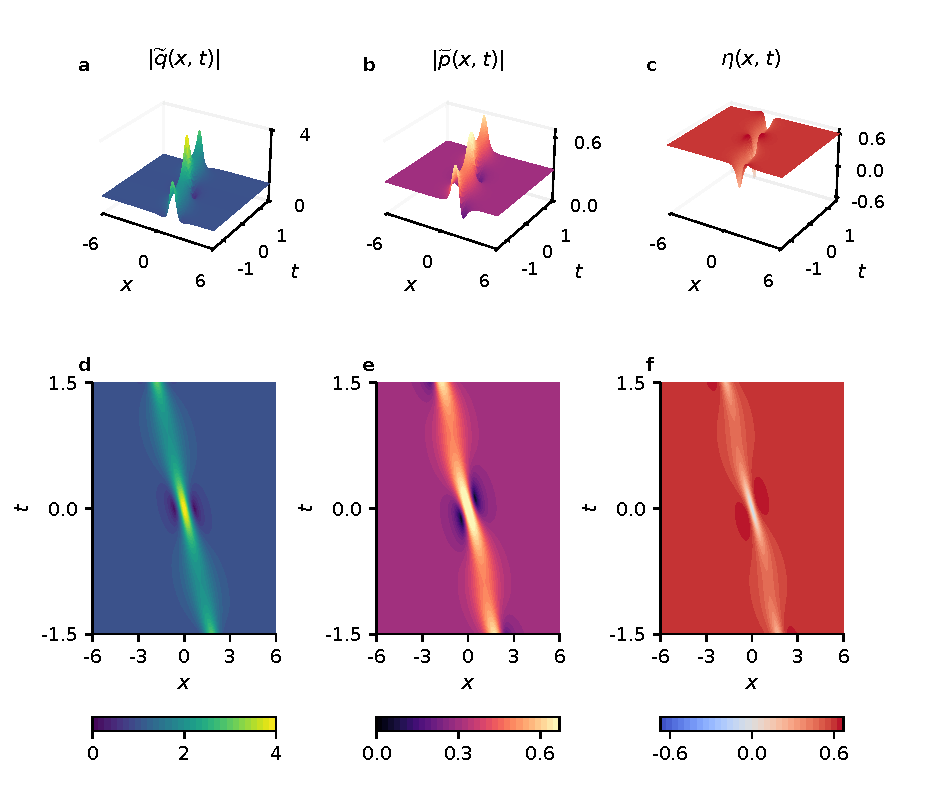
\includegraphics[width=\textwidth]{figures/one-soliton-fields.pdf}
\caption{单轨道物理三场 $|\widetilde q|,|\widetilde p|,\eta$ 的曲面 (上排) 与等值图 (下排). 参数见 \eqref{eq:numerical-parameters}; $x\in\lbrack-6,6\rbrack$, $t\in\lbrack-1.5,1.5\rbrack$.}
\label{fig:one}
\end{figure}

\FloatBarrier
\subsection{传播速度与内部振荡}
将背景传播因子分解为
\begin{align}
A_b=\operatorname{Re}F(\ii b)
&=-4\beta b^2-2\beta q_0^2-\dfrac{\eta_0}{a^2+b^2},\label{eq:velocity}\\
B_b=\operatorname{Im}F(\ii b)
&=-\alpha b-\dfrac{\eta_0b}{a(a^2+b^2)}.\label{eq:frequency}
\end{align}
\paragraph{传播函数实部和虚部的全部计算.}
从式 \eqref{eq:F} 原封不动代入 $k=\ii b$:
\begin{align*}
F(\ii b)
&=4\beta(\ii b)^2-\alpha\ii b-2\beta q_0^2
+\dfrac{\eta_0}{a(\ii b-a)}\\
&=-4\beta b^2-\ii\alpha b-2\beta q_0^2
+\dfrac{\eta_0(-a-\ii b)}{a(\ii b-a)(-a-\ii b)}.
\end{align*}
分母中
\[
(\ii b-a)(-a-\ii b)
=-\ii ab+b^2+a^2+\ii ab=a^2+b^2.
\]
所以有理项恰为
\[
\dfrac{\eta_0}{a(\ii b-a)}
=-\dfrac{\eta_0}{a^2+b^2}
-\ii\dfrac{\eta_0b}{a(a^2+b^2)}.
\]
其余各项的实虚性都已显现. 把没有 $\ii$ 的项与含 $\ii$ 的项分别合并, 就得到式 \eqref{eq:velocity}--\eqref{eq:frequency}. 因为所有参数为实数, 这里无需再对任何系数取实部或虚部. 同时
\[
F(-\ii b)=A_b-\ii B_b=\conj{F(\ii b)},
\]
与第8节使用的两个 $D_+$ 点的指数关系一致.

于是 $s=\kappa X-\ii\kappa B_bt$, 其中 $X=x-A_bt$. 显式矩阵 $P$ 关于 $x,t$ 的依赖由
\[
T=e^{2s}=e^{2\kappa X}e^{-2\ii\kappa B_bt}
\]
确定. 固定 $X$ 时, 若 $B_b\ne0$, 去相位三场具有周期
\begin{equation}\label{eq:internal-period}
T_t=\dfrac{\pi}{\kappa|B_b|}.
\end{equation}
\paragraph{包络移动和内部振荡怎样从同一个指数读出.}
不另设坐标, 先直接在原变量中展开:
\begin{align*}
s&=\kappa\{x-(A_b+\ii B_b)t\}
=\kappa(x-A_bt)-\ii\kappa B_bt,\\
2s&=2\kappa(x-A_bt)-2\ii\kappa B_bt,\\
|T|&=\left|e^{2\kappa(x-A_bt)}e^{-2\ii\kappa B_bt}\right|
=e^{2\kappa(x-A_bt)}.
\end{align*}
原文的 $X=x-A_bt$ 仅把已经出现的表达式命名, 本册没有额外变换. 要使 $|T|$ 保持相同, 就要保持 $x-A_bt$ 相同, 因而中心线是 $x=A_bt$. 同时比较 $t$ 与 $t+T_t$ 且沿这条同速轨迹移动 $x$, 有
\begin{align*}
T(x+A_bT_t,t+T_t)
&=e^{2\kappa[x+A_bT_t-A_b(t+T_t)]}
e^{-2\ii\kappa B_b(t+T_t)}\\
&=T(x,t)e^{-2\ii\kappa B_bT_t}.
\end{align*}
要让这个额外因子等于1, 其指数的相位必须是 $2\pi$ 的整数倍. 取正的完整相位周期,
\[
2\kappa|B_b|T_t=2\pi
\quad\Longrightarrow\quad
T_t=\dfrac{\pi}{\kappa|B_b|}.
\]
$P$ 是 $T,\conj{T}$ 的有理函数, $N(a)$ 是 $P$ 的矩阵多项式, 所以它们及规范三场都在这个平移后恢复原值. 这里的 $T_t$ 是原文给周期起的名称, 不是偏导数 $\partial_tT$. 本段证明了该值是一个周期, 不需要另行断言所有特殊参数下都没有更小周期.

若 $\alpha=-\dfrac{\eta_0}{a(a^2+b^2)}$, 则 $B_b=0$, 去相位三场仅依赖 $X$. 原场的模 $|\widetilde q|,|\widetilde p|$ 和反转 $\eta$ 也具有周期 \eqref{eq:internal-period}; 复场 $\widetilde q,\widetilde p$ 具有同一随动周期当且仅当 $\Omega T_t\in2\pi\mathbb Z$.

\paragraph{消除内部振荡与恢复共同相位.}
由 $b>q_0>0$ 可除以 $b$. 将 $B_b$ 的表达式设为零, 逐步得到
\begin{align*}
0&=-\alpha b-\dfrac{\eta_0b}{a(a^2+b^2)},\\
0&=-\alpha-\dfrac{\eta_0}{a(a^2+b^2)},\\
\alpha&=-\dfrac{\eta_0}{a(a^2+b^2)}.
\end{align*}
此时 $s$ 没有随 $t$ 单独变化的虚部, 所有规范场仅通过 $x-A_bt$ 变化. 这里不能把含 $|B_b|$ 的周期公式代入零分母; 正确结论是内部振荡消失.

当 $B_b\ne0$ 时, 规范场在一次随动周期后恢复, 原复光场还多出
\[
\dfrac{e^{-\ii\Omega(t+T_t)}}{e^{-\ii\Omega t}}
=e^{-\ii\Omega T_t}.
\]
由于 $q$ 有非零端态 $q_0$, 若要求整个复光场在同一次平移后恢复, 该因子必须为1. 这等价于 $\Omega T_t\in2\pi\mathbb Z$. 极化同理. 模长则不受这个因子影响, 反转本来就没有共同相位.

由 $P^2=P=P^\dagger$ 和 $\tr P=1$, 有 $|P_{12}|^2=P_{11}(1-P_{11})\le\dfrac{1}{4}$. 因而
\begin{equation}\label{eq:amplitude-bound}
|\widetilde q(x,t)|\le q_0+2b,\qquad |\widetilde q(0,0)|=q_0+2b.
\end{equation}
后一等式使用 $T(0,0)=1$ 和 $P_{12}(0,0)=\dfrac{1}{2}$. $P$ 在 $X\to\pm\infty$ 时趋于端态投影, 修正项为 $O(e^{-2\kappa|X|})$, 所以局域化尺度由 $\kappa$ 决定.

\paragraph{振幅估计每一步的不等式.}
Hermitian 性给出 $P_{21}=\conj{P_{12}}$. 取 $P^2=P$ 的第1行第1列:
\begin{align*}
P_{11}^2+P_{12}P_{21}&=P_{11},\\
|P_{12}|^2&=P_{11}-P_{11}^2
=\dfrac{1}{4}-\left(P_{11}-\dfrac{1}{2}\right)^2\le\dfrac{1}{4}.
\end{align*}
$P_{11}$ 为实数, 所以平方项非负, 从而 $|P_{12}|\le\dfrac{1}{2}$. 取式 \eqref{eq:finalfields} 中光场的模并应用三角不等式,
\begin{align*}
|\widetilde q|
&=\left|e^{-\ii\Omega t}(-q_0-4bP_{12})\right|
=|-q_0-4bP_{12}|\\
&\le q_0+4b|P_{12}|
\le q_0+2b.
\end{align*}
在 $x=t=0$ 时, 原文 $s=0$, $T=1$. 由 $\Delta_-=|T-h_0|^2+|1-h_0T|^2$,
\[
\Delta_-(0,0)=2(1-h_0)^2,
\qquad
P_{12}(0,0)=\dfrac{(1-h_0)(1-h_0)}{2(1-h_0)^2}=\dfrac{1}{2}.
\]
于是 $\widetilde q(0,0)=-q_0-2b$ 是负实数, 它的模正好达到上界. 本例等于 $1+2\cdot1.5=4$.

\paragraph{在原点同时检查两个介质分量.}
原点 $P$ 的四个元均为 $\dfrac{1}{2}$, 故式 \eqref{eq:Nfactor} 中的 $N(a)$ 在这里为
\[
N(a)=aI+\ii b(I-2P)
=\begin{pmatrix}a&-\ii b\\-\ii b&a\end{pmatrix}.
\]
将这四个元代入式 \eqref{eq:etacomponent}--\eqref{eq:pcomponent}:
\begin{align*}
\eta(0,0)
&=\dfrac{\eta_0}{a^2+b^2}
\left[a^2-b^2+\dfrac{\ii q_0}{a}
\{a(\ii b)-(-\ii b)a\}\right]\\
&=\dfrac{\eta_0}{a^2+b^2}(a^2-b^2-2bq_0),\\
\widetilde p(0,0)
&=\dfrac{\eta_0}{a^2+b^2}
\left[a(\ii b)-(-\ii b)a
+\dfrac{\ii q_0}{a}\{a^2-(-\ii b)(\ii b)\}\right]\\
&=\dfrac{\ii\eta_0}{a^2+b^2}
\left[2ab+\dfrac{q_0}{a}(a^2-b^2)\right].
\end{align*}
本例 $a^2+b^2=4+2.25=6.25$, 故
\begin{align*}
\eta(0,0)&=\dfrac{0.6}{6.25}(4-2.25-3)=-0.12,\\
\widetilde p(0,0)&=\dfrac{0.6\ii}{6.25}
\left[6+\dfrac{4-2.25}{2}\right]=0.66\ii,\\
|\widetilde p(0,0)|^2+\eta(0,0)^2
&=0.66^2+(-0.12)^2=0.4356+0.0144=0.45.
\end{align*}
因此图中中心处的介质偏离背景, 但仍严格位于同一个 Bloch 长度约束上.

\paragraph{指数衰减的量级为何是这个指数.}
由原文的 $P$ 公式, 当 $|T|\to0$ 时, 分子和分母都可以按 $T,\conj{T}$ 展开. 分母常数项是 $1+h_0^2>0$, 所以 $P-P_-$ 的每个元都是 $O(|T|)$. 当 $|T|\to\infty$ 时, 把分子分母同时除以 $|T|^2$, 常数主项给出 $P_+$, 其余是 $O(|T|^{-1})$. 又
\[
|T|=e^{2\kappa X},\qquad
|T|^{-1}=e^{-2\kappa X}.
\]
所以 $X\to-\infty$ 与 $X\to+\infty$ 的误差统一是 $O(e^{-2\kappa|X|})$. 光场是 $P$ 的线性表达式, 介质是 $P$ 的光滑有理矩阵表达式且分母 $a^2+b^2>0$, 因此三场保持同样的衰减量级.

参数 \eqref{eq:numerical-parameters} 给出 $A_b=-1.196$、$B_b=-1.572$ 和 $T_t\approx1.78748466439$. 图 \ref{fig:dynamics} 左图比较 $t=0,\dfrac{T_t}{4},\dfrac{T_t}{2}$ 时的随动截面; 右图比较 $\alpha=-0.048,0.5,1$ 时的中心光场模. 后两者的周期分别约为 $3.41840132897$ 和 $1.78748466439$, 而 $\alpha=-0.048$ 对应行波.
\paragraph{这些小数怎样算出.}
本例公共分母为 $a^2+b^2=6.25$. 逐项代入得
\begin{align*}
A_b&=-4\cdot0.1\cdot1.5^2-2\cdot0.1\cdot1^2-\dfrac{0.6}{6.25}\\
&=-0.9-0.2-0.096=-1.196,\\
B_b&=-1\cdot1.5-\dfrac{0.6\cdot1.5}{2\cdot6.25}
=-1.5-0.072=-1.572,\\
T_t&=\dfrac{\pi}{\dfrac{\sqrt{5}}{2}\cdot1.572}
\approx1.78748466439.
\end{align*}
当只把 $\alpha$ 改成 $0.5$ 时, $A_b$ 的表达式中没有 $\alpha$, 所以传播速度不变, 而
\[
B_b=-0.5\cdot1.5-0.072=-0.822,\qquad
T_t=\dfrac{\pi}{\dfrac{\sqrt{5}}{2}\cdot0.822}
\approx3.41840132897.
\]
当 $\alpha=-0.048$ 时,
\[
B_b=-(-0.048)\cdot1.5-0.072=0.072-0.072=0.
\]
同一个数也由临界参数式给出:
\[
-\dfrac{\eta_0}{a(a^2+b^2)}=-\dfrac{0.6}{2\cdot6.25}=-0.048.
\]
因此三条中心曲线的差别是内部振荡变化, 不是中心沿 $x$ 方向的移动速度变化. 图左在固定随动位置比较不同 $t$ 的截面, 正是为了能直接看见这个内部变化.
\begin{figure}[htbp]
\centering
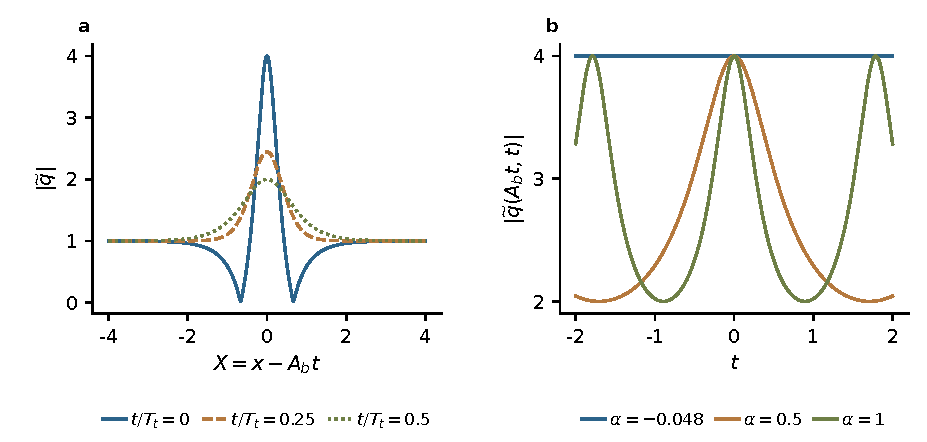
\includegraphics[width=\textwidth]{figures/one-soliton-dynamics.pdf}
\caption{单轨道光场的局域化与内部振荡. (a) 参数 \eqref{eq:numerical-parameters} 下的随动截面. (b) 改变 $\alpha$ 时 $|\widetilde q(A_bt,t)|$ 的变化, 其余参数固定.}
\label{fig:dynamics}
\end{figure}

\FloatBarrier
\subsection{参数影响与数值验证}
$\beta$ 改变式 \eqref{eq:velocity} 中的传播速度, 而不改变式 \eqref{eq:frequency} 中的内部频率. 图 \ref{fig:velocity} 取 $\beta=0,0.15$, 相应的 $A_b$ 为 $-0.096,-1.746$; 两者均有 $B_b=-1.572$ 和相同的随动周期. 虚线 $x=A_bt$ 表示中心轨迹.
\paragraph{分离两个参数作用的直接计算.}
在当前参数下, 速度对 $\beta$ 的依赖直接合并成
\[
A_b=-4\beta\cdot2.25-2\beta-0.096=-11\beta-0.096.
\]
代入图中两个取值得
\[
\beta=0:\quad A_b=-0.096,\qquad
\beta=0.15:\quad A_b=-11\cdot0.15-0.096=-1.746.
\]
两者都是负数, 所以 $t$ 增加时中心向更小的 $x$ 传播. 在固定 $q_0,a,\eta_0,b$ 下, 对原表达式求参数导数还可直接看出
\[
\dfrac{\partial A_b}{\partial\beta}=-4b^2-2q_0^2,\qquad
\dfrac{\partial B_b}{\partial\beta}=0,\qquad
\dfrac{\partial A_b}{\partial\alpha}=0,\qquad
\dfrac{\partial B_b}{\partial\alpha}=-b.
\]
因此在这个一轨道族中, 改变 $\beta$ 直接改变包络速度, 改变 $\alpha$ 直接改变内部振荡频率. 这几条参数偏导数只是原式的求导, 不需要额外的扰动理论. $\alpha$ 还通过 $\Omega$ 改变原复场的共同相位; 模长图没有显示这一相位变化.
\begin{figure}[htbp]
\centering
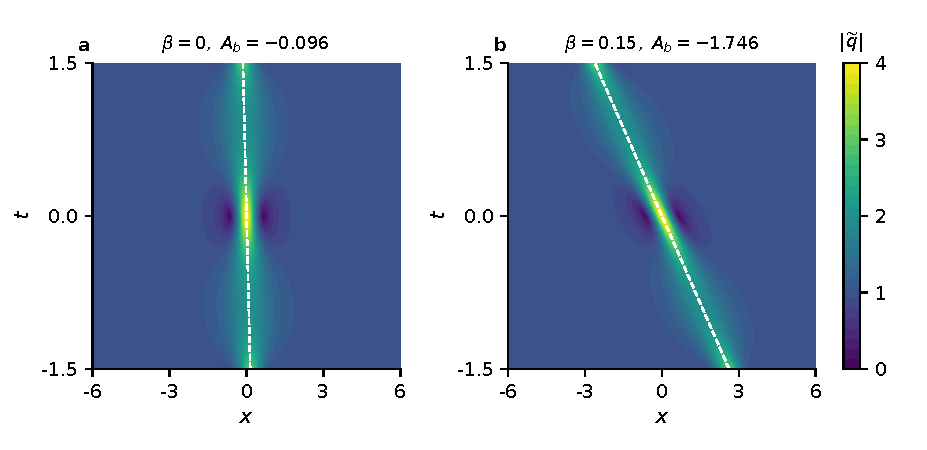
\includegraphics[width=\textwidth]{figures/one-soliton-velocity.pdf}
\caption{改变 $\beta$ 时的光场传播速度. 两图分别取 $\beta=0,0.15$, 其余参数同 \eqref{eq:numerical-parameters}; 白色虚线为 $x=A_bt$.}
\label{fig:velocity}
\end{figure}

对参数 \eqref{eq:numerical-parameters}, 采用 70 位十进制精度求解留数系统并对重构场求导, 得到表 \ref{tab:direct-residuals}. 导数由重构表达式直接计算. 双精度绘图实现与高精度实现的三个场在相同样点上的差均小于 $10^{-14}$; 等值图网格上的 Bloch 长度平方偏差及 $\eta$ 虚部均小于 $10^{-14}$. 两端 $x=\pm30$ 的三场误差均小于 $5.02\times10^{-29}$.
\begin{table}[htbp]
\centering
\caption{单轨道三场的高精度核验, 表内为样点最大绝对残差的向上舍入值}
\label{tab:direct-residuals}
\begin{tabular}{lc}
\toprule 检验对象 & 最大绝对误差\\\midrule
光场方程 & $1.87\times10^{-69}$\\
极化方程 & $8.26\times10^{-71}$\\
粒子数反转方程 & $1.50\times10^{-70}$\\
空间 Lax 方程 & $4.82\times10^{-70}$\\
时间 Lax 方程 & $1.95\times10^{-69}$\\
两共振原像的介质重构 & $1.12\times10^{-71}$\\
Bloch 长度平方 & $4.77\times10^{-72}$\\
\bottomrule
\end{tabular}
\end{table}

\paragraph{表中各行的残差究竟怎样形成.}
先在一个给定样点计算场及其所需导数, 再把方程的全部项移到左边. 表中前三行对应以下三个复数或实数的绝对值:
\begin{align*}
\left|\widetilde q_t
-\ii\alpha\left(\dfrac{\widetilde q_{xx}}{2}+|\widetilde q|^2\widetilde q\right)
-\beta(\widetilde q_{xxx}+6|\widetilde q|^2\widetilde q_x)-2\widetilde p\right|,\\
\left|\widetilde p_x-2\eta\widetilde q+2\ii a\widetilde p\right|,\\
\left|\eta_x+\conj{\widetilde q}\widetilde p+\widetilde q\conj{\widetilde p}\right|.
\end{align*}
例如, 第二条的加号来自把原方程右端的 $-2\ii a\widetilde p$ 移到左边. 它不是把原方程改成了另一个符号约定. 对每个样点各算一次, 再对所有样点取最大值, 得到表中的最大绝对残差. 在精确算术下这三项都为零; 高精度计算中的小非零值来自有限精度求值和求导.

\paragraph{原场导数与规范场导数的关系.}
共同相位只依赖 $t$, 所以所有 $x$ 导数都可以把它提出. 按原文的光场和介质重构式,
\begin{align*}
\widetilde q_x&=-4b e^{-\ii\Omega t}\partial_xP_{12},\\
\widetilde q_{xx}&=-4b e^{-\ii\Omega t}\partial_x^2P_{12},\\
\widetilde q_{xxx}&=-4b e^{-\ii\Omega t}\partial_x^3P_{12},\\
\widetilde q_t
&=e^{-\ii\Omega t}\left[\ii\Omega(q_0+4bP_{12})-4b\partial_tP_{12}\right],\\
\widetilde p_x&=-e^{-\ii\Omega t}\partial_xR_{12},\qquad
\eta_x=\partial_xR_{11}.
\end{align*}
时间导数中必须保留 $\ii\Omega(q_0+4bP_{12})$; 漏掉它就会把原方程与规范后的方程混用. 原文已有指数的导数也可直接计算:
\begin{align*}
\partial_xT&=2\kappa T,&
\partial_x\conj{T}&=2\kappa\conj{T},\\
\partial_tT&=-2\kappa F(\ii b)T,&
\partial_t\conj{T}&=-2\kappa\conj{F(\ii b)}\conj{T}.
\end{align*}
在这组式子里使用 $\partial_tT$ 表示偏导, 避免与原文的周期名称 $T_t$ 混淆. 将这些导数用于 $P$ 的原有有理表达式, 就能以乘法法则和商法则生成场导数, 不必使用网格差分.
本节末尾的``投影矩阵与三场导数的逐项求值''继续写出这些商法则的三阶展开、全部投影元的一阶导数, 以及介质矩阵的逐元导数, 可按该顺序直接执行求值.

\paragraph{两条 Lax 残差的符号.}
由式 \eqref{eq:Mspace} 及 $\phi=Me^{\ii\theta\sg}$, 对修正矩阵计算的两条残差是
\[
M_x-UM-\ii\lambda M\sg,\qquad
M_t-VM+\ii\lambda F M\sg.
\]
空间式的右乘项是负号移到左边, 时间式则因 $\theta_t=\lambda F$ 带相反的符号. 对每个谱测试点先取每个矩阵元绝对值的最大值, 再跨样点取最大值, 即得到表中两条 Lax 行. 两共振原像的核验则分别用 $z_a^+$、$z_a^-$ 代入式 \eqref{eq:RfromM}, 取两个矩阵之差的最大元绝对值. Bloch 行直接计算
\[
\left||\widetilde p|^2+\eta^2-
\eta_0^2\left(1+\dfrac{q_0^2}{a^2}\right)\right|.
\]

\paragraph{误差量级与边界检查怎样解释.}
70位十进制精度是内部运算的精度设定, 不是说每个结果都有70位相对有效数字. 对接近零的残差, 表格报告的是绝对误差. ``向上舍入''表示显示值不低于本次样点计算的最大值. 原文表格保留底稿的数值; 本详细版的复核结果另存于工程的检查报告中, 不把一次重跑得到的末位变化写成新的解析结论.
其中三条 PDE、两条 Lax 方程、留数系统和两共振重构的本次高精度结果保存在
\texttt{calculations/direct-rhp-results.json}; 原点三场、传播参数及指数因子保存在
\texttt{calculations/expanded-numerics-check.json}. 原文所述完整绘图网格误差按底稿保留, 本次没有重新生成全部网格和图像.

本例 $\kappa=\dfrac{\sqrt{5}}{2}$, 所以固定 $t$ 时理论端态衰减含有因子 $e^{-\sqrt{5}|x|}$. 在 $|x|=30$ 时,
\[
e^{-2\kappa\cdot30}=e^{-30\sqrt{5}}\approx7.36\times10^{-30}.
\]
这只是指数部分的数量级, 还要乘上依赖固定 $t$ 和场分量的有限系数, 所以不能直接把它当作三场误差的共同上界. 实际边界检查分别计算
\[
|\widetilde q-q_0e^{-\ii\Omega t}|,\qquad
\left|\widetilde p+\dfrac{\ii\eta_0q_0}{a}e^{-\ii\Omega t}\right|,\qquad
|\eta-\eta_0|.
\]
解析证明说明对所有允许参数和全部实 $x,t$ 的结构结论, 数值检查则检验本次实现是否在具体样点上正确执行了公式. 两者在本节中的作用由此区分.

\subsubsection*{补充计算: 投影矩阵与三场导数的逐项求值}
这一段继续使用原文的 $T,h_0,\kappa,\Delta_-,P,N,n_{jk}$, 不为任何分子或分母另取名称. 求偏导时固定全部模型参数和离散谱参数. 下面所有式子都只含原文已经定义的量及它们的导数, 所以既可以手工依次计算, 也可以按所写顺序直接用于数值求值.

\paragraph{先展开模平方及其空间、时间导数.}
原有指数满足
\begin{align*}
\partial_xT&=2\kappa T,
&\partial_x\conj{T}&=2\kappa\conj{T},\\
\partial_tT&=-2\kappa F(\ii b)T,
&\partial_t\conj{T}&=-2\kappa\conj{F(\ii b)}\conj{T}.
\end{align*}
因此不能把 $|T|^2$ 当成常数, 而须按两个指数的乘积求导:
\begin{align*}
|T|^2&=T\conj{T},\\
\partial_x|T|^2
&=(2\kappa T)\conj{T}
+T(2\kappa\conj{T})=4\kappa|T|^2,\\
\partial_x^2|T|^2
&=4\kappa\partial_x|T|^2
=16\kappa^2|T|^2,\\
\partial_x^3|T|^2
&=16\kappa^2\partial_x|T|^2
=64\kappa^3|T|^2,\\
\partial_t|T|^2
&=-2\kappa F(\ii b)T\conj{T}
-2\kappa\conj{F(\ii b)}T\conj{T}\\
&=-2\kappa\bigl(F(\ii b)+\conj{F(\ii b)}\bigr)|T|^2.
\end{align*}
同样, 对两个一次指数分别有
\begin{align*}
\partial_x^2T&=4\kappa^2T,
&\partial_x^2\conj{T}&=4\kappa^2\conj{T},\\
\partial_x^3T&=8\kappa^3T,
&\partial_x^3\conj{T}&=8\kappa^3\conj{T}.
\end{align*}
模平方的空间导数系数是 $4\kappa$, 一次指数的系数则是 $2\kappa$, 后面出现的 $2,4,8$ 倍数正是由这一区别产生.

\paragraph{把原分母的所有所需导数写全.}
原分母不作换名, 直接展开为
\[
\Delta_-=(1+h_0^2)(1+|T|^2)-2h_0(T+\conj{T}).
\]
连续求三次 $x$ 导数, 得
\begin{align*}
\partial_x\Delta_-
&=(1+h_0^2)\partial_x|T|^2
-2h_0(\partial_xT+\partial_x\conj{T})\\
&=4\kappa(1+h_0^2)|T|^2
-4\kappa h_0(T+\conj{T}),\\
\partial_x^2\Delta_-
&=4\kappa(1+h_0^2)\partial_x|T|^2
-4\kappa h_0(\partial_xT+\partial_x\conj{T})\\
&=16\kappa^2(1+h_0^2)|T|^2
-8\kappa^2h_0(T+\conj{T}),\\
\partial_x^3\Delta_-
&=16\kappa^2(1+h_0^2)\partial_x|T|^2
-8\kappa^2h_0(\partial_xT+\partial_x\conj{T})\\
&=64\kappa^3(1+h_0^2)|T|^2
-16\kappa^3h_0(T+\conj{T}).
\end{align*}
时间导数则保留原有传播函数及其共轭:
\begin{align*}
\partial_t\Delta_-
&=(1+h_0^2)\partial_t|T|^2
-2h_0(\partial_tT+\partial_t\conj{T})\\
&=-2\kappa(1+h_0^2)
\bigl(F(\ii b)+\conj{F(\ii b)}\bigr)|T|^2\\
&\quad+4\kappa h_0
\bigl(F(\ii b)T+\conj{F(\ii b)}\conj{T}\bigr).
\end{align*}
这些式子都可以只用已知的 $T,\conj{T}$ 直接求值. 后面出现 $\partial_x\Delta_-$ 等记法时, 它们就是以上完全写出的表达式, 并不代表需要另外求解的未知量.

\paragraph{右上投影元的乘积恒等式及其各阶右端.}
从原投影公式开始,
\begin{align*}
\Delta_-P_{12}
&=(T-h_0)(1-h_0\conj{T})\\
&=T-h_0-h_0|T|^2+h_0^2\conj{T}.
\end{align*}
右端的一至三阶空间导数依次是
\begin{align*}
\partial_x\bigl[(T-h_0)(1-h_0\conj{T})\bigr]
&=2\kappa T-4\kappa h_0|T|^2
+2\kappa h_0^2\conj{T}\\
&=2\kappa\bigl(T+h_0^2\conj{T}-2h_0|T|^2\bigr),\\
\partial_x^2\bigl[(T-h_0)(1-h_0\conj{T})\bigr]
&=4\kappa^2T-16\kappa^2h_0|T|^2
+4\kappa^2h_0^2\conj{T}\\
&=4\kappa^2\bigl(T+h_0^2\conj{T}-4h_0|T|^2\bigr),\\
\partial_x^3\bigl[(T-h_0)(1-h_0\conj{T})\bigr]
&=8\kappa^3T-64\kappa^3h_0|T|^2
+8\kappa^3h_0^2\conj{T}\\
&=8\kappa^3\bigl(T+h_0^2\conj{T}-8h_0|T|^2\bigr).
\end{align*}
时间导数也从原乘积直接展开:
\begin{align*}
\partial_t\bigl[(T-h_0)(1-h_0\conj{T})\bigr]
&=(-2\kappa F(\ii b)T)(1-h_0\conj{T})\\
&\quad+(T-h_0)
\bigl(2\kappa h_0\conj{F(\ii b)}\conj{T}\bigr)\\
&=-2\kappa F(\ii b)T
+2\kappa h_0F(\ii b)|T|^2\\
&\quad+2\kappa h_0\conj{F(\ii b)}|T|^2
-2\kappa h_0^2\conj{F(\ii b)}\conj{T}\\
&=-2\kappa\left[
F(\ii b)T+h_0^2\conj{F(\ii b)}\conj{T}
-h_0\bigl(F(\ii b)+\conj{F(\ii b)}\bigr)|T|^2
\right].
\end{align*}

\paragraph{由乘积恒等式连续求导, 得到可依次执行的递推.}
对 $\Delta_-P_{12}$ 求一次导数时, 两个因子都要求导:
\[
\Delta_-\partial_xP_{12}
+(\partial_x\Delta_-)P_{12}
=2\kappa\bigl(T+h_0^2\conj{T}-2h_0|T|^2\bigr).
\]
再求一次导数, 有
\begin{align*}
\Delta_-\partial_x^2P_{12}
+2(\partial_x\Delta_-)\partial_xP_{12}
+(\partial_x^2\Delta_-)P_{12}
&=4\kappa^2
\bigl(T+h_0^2\conj{T}-4h_0|T|^2\bigr).
\end{align*}
这里两个相同的中间项分别来自对 $\Delta_-\partial_xP_{12}$ 和 $(\partial_x\Delta_-)P_{12}$ 求导. 第三次求导时,
\begin{align*}
\Delta_-\partial_x^3P_{12}
&+3(\partial_x\Delta_-)\partial_x^2P_{12}\\
&+3(\partial_x^2\Delta_-)\partial_xP_{12}
+(\partial_x^3\Delta_-)P_{12}\\
&=8\kappa^3
\bigl(T+h_0^2\conj{T}-8h_0|T|^2\bigr).
\end{align*}
因此实际求值时可以按以下顺序, 每次只使用前面已经算出的低阶导数:
\begin{align*}
\partial_xP_{12}
&=\dfrac{2\kappa(T+h_0^2\conj{T}-2h_0|T|^2)
-(\partial_x\Delta_-)P_{12}}{\Delta_-},\\
\partial_x^2P_{12}
&=\dfrac{4\kappa^2(T+h_0^2\conj{T}-4h_0|T|^2)}{\Delta_-}\\
&\quad-\dfrac{2(\partial_x\Delta_-)\partial_xP_{12}
+(\partial_x^2\Delta_-)P_{12}}{\Delta_-},\\
\partial_x^3P_{12}
&=\dfrac{8\kappa^3(T+h_0^2\conj{T}-8h_0|T|^2)}{\Delta_-}\\
&\quad-\dfrac{3(\partial_x\Delta_-)\partial_x^2P_{12}
+3(\partial_x^2\Delta_-)\partial_xP_{12}
+(\partial_x^3\Delta_-)P_{12}}{\Delta_-}.
\end{align*}
原文已经证明 $\Delta_->0$, 所以每一次除法在所有实 $x,t$ 上都有意义. 这个递推没有引入分子的新名字, 也不需要用相邻网格点近似导数.

\paragraph{把递推消去, 写成完全展开的商法则形式.}
先把原 $P_{12}$ 代入一次导数公式:
\begin{align*}
\partial_xP_{12}
&=\dfrac{2\kappa(T+h_0^2\conj{T}-2h_0|T|^2)}{\Delta_-}\\
&\quad-\dfrac{(T-h_0)(1-h_0\conj{T})\partial_x\Delta_-}{\Delta_-^2}.
\end{align*}
对这一行逐项再求导, 相同项合并后得到
\begin{align*}
\partial_x^2P_{12}
&=\dfrac{4\kappa^2(T+h_0^2\conj{T}-4h_0|T|^2)}{\Delta_-}\\
&\quad-\dfrac{4\kappa(T+h_0^2\conj{T}-2h_0|T|^2)
\partial_x\Delta_-}{\Delta_-^2}\\
&\quad-\dfrac{(T-h_0)(1-h_0\conj{T})
\partial_x^2\Delta_-}{\Delta_-^2}\\
&\quad+\dfrac{2(T-h_0)(1-h_0\conj{T})
(\partial_x\Delta_-)^2}{\Delta_-^3}.
\end{align*}
再对各项求导, 三阶结果为
\begin{align*}
\partial_x^3P_{12}
&=\dfrac{8\kappa^3(T+h_0^2\conj{T}-8h_0|T|^2)}{\Delta_-}\\
&\quad-\dfrac{12\kappa^2(T+h_0^2\conj{T}-4h_0|T|^2)
\partial_x\Delta_-}{\Delta_-^2}\\
&\quad-\dfrac{6\kappa(T+h_0^2\conj{T}-2h_0|T|^2)
\partial_x^2\Delta_-}{\Delta_-^2}\\
&\quad+\dfrac{12\kappa(T+h_0^2\conj{T}-2h_0|T|^2)
(\partial_x\Delta_-)^2}{\Delta_-^3}\\
&\quad-\dfrac{(T-h_0)(1-h_0\conj{T})
\partial_x^3\Delta_-}{\Delta_-^2}\\
&\quad+\dfrac{6(T-h_0)(1-h_0\conj{T})
(\partial_x\Delta_-)(\partial_x^2\Delta_-)}{\Delta_-^3}\\
&\quad-\dfrac{6(T-h_0)(1-h_0\conj{T})
(\partial_x\Delta_-)^3}{\Delta_-^4}.
\end{align*}
这两种写法完全等价: 递推形式依次利用低阶结果, 展开形式则只有 $T,\conj{T}$、原分母及其已写出的导数. 例如三阶式中的系数3, 来自第三次对乘积求导时导数分配到两个因子的三种位置; 展开后对应系数 $12\kappa^2$, $6\kappa$, $12\kappa$.

\paragraph{右上投影元的时间导数.}
对原乘积恒等式求 $t$ 导数, 先得到
\begin{align*}
\Delta_-\partial_tP_{12}
+(\partial_t\Delta_-)P_{12}
&=-2\kappa\left[
F(\ii b)T+h_0^2\conj{F(\ii b)}\conj{T}\right.\\
&\hspace{35mm}\left.
-h_0\bigl(F(\ii b)+\conj{F(\ii b)}\bigr)|T|^2
\right].
\end{align*}
移项并代回原 $P_{12}$, 就有
\begin{align*}
\partial_tP_{12}
&=-\dfrac{2\kappa}{\Delta_-}
\left[F(\ii b)T+h_0^2\conj{F(\ii b)}\conj{T}\right.\\
&\hspace{34mm}\left.
-h_0\bigl(F(\ii b)+\conj{F(\ii b)}\bigr)|T|^2\right]\\
&\quad-\dfrac{(T-h_0)(1-h_0\conj{T})
\partial_t\Delta_-}{\Delta_-^2}.
\end{align*}
原场所需导数于是全部可以直接算出:
\begin{align*}
\widetilde q_x
&=-4b e^{-\ii\Omega t}\partial_xP_{12},\\
\widetilde q_{xx}
&=-4b e^{-\ii\Omega t}\partial_x^2P_{12},\\
\widetilde q_{xxx}
&=-4b e^{-\ii\Omega t}\partial_x^3P_{12},\\
\widetilde q_t
&=e^{-\ii\Omega t}
\left[\ii\Omega(q_0+4bP_{12})-4b\partial_tP_{12}\right].
\end{align*}
这里时间导数中的共同相位项仍须保留; 以上投影导数本身不能替代它.

\paragraph{其余三个投影元的一阶空间导数.}
先把原分子逐个展开, 不给它们另起名字:
\begin{align*}
|T-h_0|^2&=|T|^2-h_0(T+\conj{T})+h_0^2,\\
(1-h_0T)(\conj{T}-h_0)
&=\conj{T}-h_0-h_0|T|^2+h_0^2T,\\
|1-h_0T|^2&=1-h_0(T+\conj{T})+h_0^2|T|^2.
\end{align*}
故它们的导数分别为
\begin{align*}
\partial_x|T-h_0|^2
&=4\kappa|T|^2-2\kappa h_0(T+\conj{T}),\\
\partial_x\bigl[(1-h_0T)(\conj{T}-h_0)\bigr]
&=2\kappa\bigl(\conj{T}+h_0^2T-2h_0|T|^2\bigr),\\
\partial_x|1-h_0T|^2
&=-2\kappa h_0(T+\conj{T})+4\kappa h_0^2|T|^2.
\end{align*}
逐个应用商法则, 得
\begin{align*}
\partial_xP_{11}
&=\dfrac{4\kappa|T|^2-2\kappa h_0(T+\conj{T})}{\Delta_-}
-\dfrac{|T-h_0|^2\partial_x\Delta_-}{\Delta_-^2},\\
\partial_xP_{21}
&=\dfrac{2\kappa(\conj{T}+h_0^2T-2h_0|T|^2)}{\Delta_-}\\
&\quad-\dfrac{(1-h_0T)(\conj{T}-h_0)
\partial_x\Delta_-}{\Delta_-^2},\\
\partial_xP_{22}
&=\dfrac{-2\kappa h_0(T+\conj{T})+4\kappa h_0^2|T|^2}{\Delta_-}
-\dfrac{|1-h_0T|^2\partial_x\Delta_-}{\Delta_-^2}.
\end{align*}
因为 $\Delta_-$ 是实函数, 可直接从这些表达式检查
\[
\partial_xP_{21}=\conj{\partial_xP_{12}},
\qquad
\partial_xP_{11}+\partial_xP_{22}=0.
\]
第二式也可以从 $P_{11}+P_{22}=1$ 求导得到, 因而是检查实际实现的一项独立恒等式.

\paragraph{其余三个投影元的一阶时间导数.}
同样先求原分子的导数:
\begin{align*}
\partial_t|T-h_0|^2
&=-2\kappa\bigl(F(\ii b)+\conj{F(\ii b)}\bigr)|T|^2\\
&\quad+2\kappa h_0
\bigl(F(\ii b)T+\conj{F(\ii b)}\conj{T}\bigr),\\
\partial_t\bigl[(1-h_0T)(\conj{T}-h_0)\bigr]
&=-2\kappa\left[
\conj{F(\ii b)}\conj{T}+h_0^2F(\ii b)T\right.\\
&\hspace{29mm}\left.
-h_0\bigl(F(\ii b)+\conj{F(\ii b)}\bigr)|T|^2\right],\\
\partial_t|1-h_0T|^2
&=2\kappa h_0
\bigl(F(\ii b)T+\conj{F(\ii b)}\conj{T}\bigr)\\
&\quad-2\kappa h_0^2
\bigl(F(\ii b)+\conj{F(\ii b)}\bigr)|T|^2.
\end{align*}
再除以原分母并减去分母求导项:
\begin{align*}
\partial_tP_{11}
&=-\dfrac{2\kappa(F(\ii b)+\conj{F(\ii b)})|T|^2}{\Delta_-}\\
&\quad+\dfrac{2\kappa h_0
(F(\ii b)T+\conj{F(\ii b)}\conj{T})}{\Delta_-}
-\dfrac{|T-h_0|^2\partial_t\Delta_-}{\Delta_-^2},\\
\partial_tP_{21}
&=-\dfrac{2\kappa}{\Delta_-}
\left[\conj{F(\ii b)}\conj{T}+h_0^2F(\ii b)T\right.\\
&\hspace{33mm}\left.
-h_0(F(\ii b)+\conj{F(\ii b)})|T|^2\right]\\
&\quad-\dfrac{(1-h_0T)(\conj{T}-h_0)
\partial_t\Delta_-}{\Delta_-^2},\\
\partial_tP_{22}
&=\dfrac{2\kappa h_0
(F(\ii b)T+\conj{F(\ii b)}\conj{T})}{\Delta_-}\\
&\quad-\dfrac{2\kappa h_0^2
(F(\ii b)+\conj{F(\ii b)})|T|^2}{\Delta_-}
-\dfrac{|1-h_0T|^2\partial_t\Delta_-}{\Delta_-^2}.
\end{align*}
它们满足 $\partial_tP_{21}=\conj{\partial_tP_{12}}$ 及 $\partial_tP_{11}+\partial_tP_{22}=0$. 因而需要时间 Lax 检查时, 原矩阵 $P$ 的全部一阶时间导数也已具备.

\paragraph{从投影导数逐元得到 $N(a)$ 的导数.}
原定义 $N(k)=(k+\ii b)I-2\ii bP$ 在 $k=a$ 时给出
\begin{align*}
n_{11}&=a+\ii b-2\ii bP_{11},
&n_{12}&=-2\ii bP_{12},\\
n_{21}&=-2\ii bP_{21},
&n_{22}&=a+\ii b-2\ii bP_{22}.
\end{align*}
因此逐元求导的结果为
\begin{align*}
\partial_xn_{11}&=-2\ii b\partial_xP_{11},
&\partial_xn_{12}&=-2\ii b\partial_xP_{12},\\
\partial_xn_{21}&=-2\ii b\partial_xP_{21},
&\partial_xn_{22}&=-2\ii b\partial_xP_{22}.
\end{align*}
将它们合为矩阵, 得
\[
\partial_xN(a)=-2\ii b\partial_xP.
\]
由于 $b$ 为实数且 $P^\dagger=P$, 求导与共轭转置交换, 所以
\begin{align*}
\partial_xN(a)^\dagger
&=(\partial_xN(a))^\dagger\\
&=(-2\ii b\partial_xP)^\dagger
=2\ii b\partial_xP.
\end{align*}
逐个标量共轭时, 同样应使用
\[
\conj{\partial_xn_{jk}}
=2\ii b\conj{\partial_xP_{jk}}.
\]
这里 $n_{jk}$ 是原论文已有的 $N(a)$ 元素, 没有引入一个新的场或新的系数矩阵.

\paragraph{介质矩阵求导时的两个乘积及非对角负号.}
原介质矩阵为
\[
R=\dfrac{HN(a)R_\infty N(a)^\dagger H^{-1}}{a^2+b^2},
\qquad H=\diag(\ii,-\ii).
\]
$H,R_\infty,a,b$ 对 $x$ 都是常数, 所以乘积法则严格给出
\[
R_x=\dfrac{H\left[
(\partial_xN(a))R_\infty N(a)^\dagger
+N(a)R_\infty(\partial_xN(a))^\dagger
\right]H^{-1}}{a^2+b^2}.
\]
这个式子包含两项, 分别来自左右两个 $N$ 因子, 不可以只对左边的因子求导. 在 $H$ 的对角共轭作用下, 对角元不变, 两个非对角元反号. 特别地,
\begin{align*}
(R_x)_{11}
&=\dfrac{\left[
(\partial_xN(a))R_\infty N(a)^\dagger
+N(a)R_\infty(\partial_xN(a))^\dagger
\right]_{11}}{a^2+b^2},\\
(R_x)_{12}
&=-\dfrac{\left[
(\partial_xN(a))R_\infty N(a)^\dagger
+N(a)R_\infty(\partial_xN(a))^\dagger
\right]_{12}}{a^2+b^2}.
\end{align*}
结合原物理场 $\widetilde p=-e^{-\ii\Omega t}R_{12}$, 这个非对角负号与恢复极化的负号相消:
\begin{align*}
\eta_x&=(R_x)_{11},\\
\widetilde p_x
&=\dfrac{e^{-\ii\Omega t}}{a^2+b^2}
\left[
(\partial_xN(a))R_\infty N(a)^\dagger
+N(a)R_\infty(\partial_xN(a))^\dagger
\right]_{12}.
\end{align*}
这解释了为什么以下极化导数公式整体带正号, 虽然 $R$ 的右上元在原定义中等于 $-p$.

\paragraph{反转导数按原 $n_{jk}$ 分量式完全展开.}
由式 \eqref{eq:etacomponent}, 对每个乘积的两个因子分别求导, 得
\begin{align*}
\eta_x
&=\dfrac{\eta_0}{a^2+b^2}\left[
(\partial_xn_{11})\conj{n_{11}}
+n_{11}\conj{\partial_xn_{11}}\right.\\
&\quad-(\partial_xn_{12})\conj{n_{12}}
-n_{12}\conj{\partial_xn_{12}}\\
&\quad+\dfrac{\ii q_0}{a}\bigl(
(\partial_xn_{11})\conj{n_{12}}
+n_{11}\conj{\partial_xn_{12}}\\
&\hspace{32mm}\left.
-(\partial_xn_{12})\conj{n_{11}}
-n_{12}\conj{\partial_xn_{11}}\bigr)\right].
\end{align*}
再用已经得到的四个 $\partial_xn_{jk}$ 消去这些导数, 可以写成
\begin{align*}
\eta_x
&=\dfrac{2\ii b\eta_0}{a^2+b^2}\left[
-(\partial_xP_{11})\conj{n_{11}}
+n_{11}\conj{\partial_xP_{11}}\right.\\
&\quad+(\partial_xP_{12})\conj{n_{12}}
-n_{12}\conj{\partial_xP_{12}}\\
&\quad+\dfrac{\ii q_0}{a}\bigl(
-(\partial_xP_{11})\conj{n_{12}}
+n_{11}\conj{\partial_xP_{12}}\\
&\hspace{32mm}\left.
+(\partial_xP_{12})\conj{n_{11}}
-n_{12}\conj{\partial_xP_{11}}\bigr)\right].
\end{align*}
虽然这个写法显式含有 $\ii$, 整体仍为实数, 因为它与 Hermitian 矩阵 $R_x$ 的对角元相同. 实际计算中出现的极小虚部可以作为舍入误差的监测量, 不应先在代数推导中随意删去一项.

\paragraph{极化导数按原 $n_{jk}$ 分量式完全展开.}
由于 $e^{\ii\Omega t}$ 不依赖 $x$, 对式 \eqref{eq:pcomponent} 求导得到
\begin{align*}
\widetilde p_x
&=\dfrac{\eta_0e^{-\ii\Omega t}}{a^2+b^2}\left[
(\partial_xn_{11})\conj{n_{21}}
+n_{11}\conj{\partial_xn_{21}}\right.\\
&\quad-(\partial_xn_{12})\conj{n_{22}}
-n_{12}\conj{\partial_xn_{22}}\\
&\quad+\dfrac{\ii q_0}{a}\bigl(
(\partial_xn_{11})\conj{n_{22}}
+n_{11}\conj{\partial_xn_{22}}\\
&\hspace{32mm}\left.
-(\partial_xn_{12})\conj{n_{21}}
-n_{12}\conj{\partial_xn_{21}}\bigr)\right].
\end{align*}
继续代入 $\partial_xn_{jk}=-2\ii b\partial_xP_{jk}$, 得
\begin{align*}
\widetilde p_x
&=\dfrac{2\ii b\eta_0e^{-\ii\Omega t}}{a^2+b^2}\left[
-(\partial_xP_{11})\conj{n_{21}}
+n_{11}\conj{\partial_xP_{21}}\right.\\
&\quad+(\partial_xP_{12})\conj{n_{22}}
-n_{12}\conj{\partial_xP_{22}}\\
&\quad+\dfrac{\ii q_0}{a}\bigl(
-(\partial_xP_{11})\conj{n_{22}}
+n_{11}\conj{\partial_xP_{22}}\\
&\hspace{32mm}\left.
+(\partial_xP_{12})\conj{n_{21}}
-n_{12}\conj{\partial_xP_{21}}\bigr)\right].
\end{align*}
右端的每个投影导数都已经由前面的商法则明示. 因而检查介质 PDE 时, 可以先从显式场求导, 再与 $2\eta\widetilde q-2\ii a\widetilde p$ 及 $-(\conj{\widetilde q}\widetilde p+\widetilde q\conj{\widetilde p})$ 比较; 不必预先把待检查的 PDE 当作计算导数的公式.

\subsubsection*{补充计算: 投影端态误差的四个分量}
\paragraph{先以减去端态并通分的方式计算, 不只读出极限.}
原文给出的两个端态投影是
\[
P_- =\dfrac{1}{1+h_0^2}
\begin{pmatrix}h_0^2&-h_0\\-h_0&1\end{pmatrix},
\qquad
P_+ =\dfrac{1}{1+h_0^2}
\begin{pmatrix}1&-h_0\\-h_0&h_0^2\end{pmatrix}.
\]
例如在负端, 第1行第1列的差通分后为
\begin{align*}
P_{11}-(P_-)_{11}
&=\dfrac{|T-h_0|^2}{\Delta_-}-\dfrac{h_0^2}{1+h_0^2}\\
&=\dfrac{(1+h_0^2)|T-h_0|^2-h_0^2\Delta_-}
{(1+h_0^2)\Delta_-}.
\end{align*}
这个分子完全展开并抵消常数项, 得
\begin{align*}
&(1+h_0^2)\bigl[|T|^2-h_0(T+\conj{T})+h_0^2\bigr]\\
&\quad-h_0^2\bigl[(1+h_0^2)(1+|T|^2)-2h_0(T+\conj{T})\bigr]\\
&=(1-h_0^2)\bigl[(1+h_0^2)|T|^2-h_0(T+\conj{T})\bigr].
\end{align*}
非对角元的相同计算是
\begin{align*}
P_{12}-(P_-)_{12}
&=\dfrac{(T-h_0)(1-h_0\conj{T})}{\Delta_-}
+\dfrac{h_0}{1+h_0^2}\\
&=\dfrac{(1+h_0^2)(T-h_0-h_0|T|^2+h_0^2\conj{T})
+h_0\Delta_-}{(1+h_0^2)\Delta_-}\\
&=\dfrac{(1-h_0^2)(T-h_0^2\conj{T})}
{(1+h_0^2)\Delta_-}.
\end{align*}
因此负端的四个差值全部为
\begin{align*}
P_{11}-(P_-)_{11}
&=\dfrac{(1-h_0^2)
\bigl[T((1+h_0^2)\conj{T}-h_0)-h_0\conj{T}\bigr]}
{(1+h_0^2)\Delta_-},\\
P_{12}-(P_-)_{12}
&=\dfrac{(1-h_0^2)(T-h_0^2\conj{T})}
{(1+h_0^2)\Delta_-},\\
P_{21}-(P_-)_{21}
&=\dfrac{(1-h_0^2)(\conj{T}-h_0^2T)}
{(1+h_0^2)\Delta_-},\\
P_{22}-(P_-)_{22}
&=-\dfrac{(1-h_0^2)
\bigl[T((1+h_0^2)\conj{T}-h_0)-h_0\conj{T}\bigr]}
{(1+h_0^2)\Delta_-}.
\end{align*}
每个分子都明确带有 $T$ 或 $\conj{T}$ 因子. 在 $|T|\to0$ 时, 分母趋于 $(1+h_0^2)^2>0$, 所以四个差值逐个都是 $O(|T|)$.

\paragraph{正端也先给出精确差值.}
两个端态的非对角元相同, 故两条非对角差值与刚才完全一致. 对角元则得到
\begin{align*}
P_{11}-(P_+)_{11}
&=\dfrac{(1+h_0^2)|T-h_0|^2-\Delta_-}
{(1+h_0^2)\Delta_-}\\
&=\dfrac{(1-h_0^2)
\bigl[h_0(T+\conj{T})-(1+h_0^2)\bigr]}
{(1+h_0^2)\Delta_-},\\
P_{12}-(P_+)_{12}
&=\dfrac{(1-h_0^2)(T-h_0^2\conj{T})}
{(1+h_0^2)\Delta_-},\\
P_{21}-(P_+)_{21}
&=\dfrac{(1-h_0^2)(\conj{T}-h_0^2T)}
{(1+h_0^2)\Delta_-},\\
P_{22}-(P_+)_{22}
&=-\dfrac{(1-h_0^2)
\bigl[h_0(T+\conj{T})-(1+h_0^2)\bigr]}
{(1+h_0^2)\Delta_-}.
\end{align*}
在 $|T|\to\infty$ 时, 必须比较分子与分母的阶数, 不能看到分子也增长就断言误差不衰减. 先把原分母除以 $|T|^2$, 得
\[
\dfrac{\Delta_-}{|T|^2}
=(1+h_0^2)\left(1+\dfrac{1}{|T|^2}\right)
-2h_0\left(\dfrac{1}{T}+\dfrac{1}{\conj{T}}\right).
\]
其中用了 $\dfrac{T}{|T|^2}=\dfrac{1}{\conj{T}}$ 和 $\dfrac{\conj{T}}{|T|^2}=\dfrac{1}{T}$. 将四个差值的分子分母同时除以 $|T|^2$, 它们逐个变成
\begin{align*}
P_{11}-(P_+)_{11}
&=\dfrac{(1-h_0^2)
\left[h_0\left(\dfrac{1}{T}+\dfrac{1}{\conj{T}}\right)
-\dfrac{1+h_0^2}{|T|^2}\right]}
{(1+h_0^2)\dfrac{\Delta_-}{|T|^2}},\\
P_{12}-(P_+)_{12}
&=\dfrac{(1-h_0^2)
\left(\dfrac{1}{\conj{T}}-\dfrac{h_0^2}{T}\right)}
{(1+h_0^2)\dfrac{\Delta_-}{|T|^2}},\\
P_{21}-(P_+)_{21}
&=\dfrac{(1-h_0^2)
\left(\dfrac{1}{T}-\dfrac{h_0^2}{\conj{T}}\right)}
{(1+h_0^2)\dfrac{\Delta_-}{|T|^2}},\\
P_{22}-(P_+)_{22}
&=-\dfrac{(1-h_0^2)
\left[h_0\left(\dfrac{1}{T}+\dfrac{1}{\conj{T}}\right)
-\dfrac{1+h_0^2}{|T|^2}\right]}
{(1+h_0^2)\dfrac{\Delta_-}{|T|^2}}.
\end{align*}
现在分子明确含有 $1/T$, $1/\conj{T}$ 或 $1/|T|^2$, 分母趋于 $(1+h_0^2)^2>0$. 因而正端的四个差值逐个都是 $O(|T|^{-1})$. 这也是在较大 $|T|$ 处求值时可用的精确等价表达式, 可以避免先形成过大的共同因子再相除.

\paragraph{从投影误差具体传递到三个场.}
两端都有 $(P_\pm)_{12}=-h_0/(1+h_0^2)$, 而原恒等式 $2bh_0=q_0(1+h_0^2)$ 给出
\[
-q_0-4b(P_\pm)_{12}
=-q_0+\dfrac{4bh_0}{1+h_0^2}
=-q_0+2q_0=q_0.
\]
所以光场的端态差精确为
\[
\widetilde q-q_0e^{-\ii\Omega t}
=-4b e^{-\ii\Omega t}
\bigl(P_{12}-(P_\pm)_{12}\bigr).
\]
对介质使用原来的 $N_\pm=(a+\ii b)I-2\ii bP_\pm$, 有
\[
N(a)-N_\pm=-2\ii b(P-P_\pm).
\]
将两个乘积相减, 可以不遗漏任何交叉项地写成
\begin{align*}
&N(a)R_\infty N(a)^\dagger-N_\pm R_\infty N_\pm^\dagger\\
&\quad=(N(a)-N_\pm)R_\infty N(a)^\dagger
+N_\pm R_\infty(N(a)^\dagger-N_\pm^\dagger).
\end{align*}
右边展开后中间的 $-N_\pm R_\infty N(a)^\dagger$ 和 $+N_\pm R_\infty N(a)^\dagger$ 相消, 正好只留下左边的两项. 再使用前文已证明的端态介质等式, 就有
\begin{align*}
R-R_\infty
&=\dfrac{1}{a^2+b^2}H\Bigl[
(N(a)-N_\pm)R_\infty N(a)^\dagger\\
&\hspace{22mm}+N_\pm R_\infty(N(a)^\dagger-N_\pm^\dagger)
\Bigr]H^{-1}.
\end{align*}
再把 $N(a)-N_\pm=-2\ii b(P-P_\pm)$ 及其 Hermitian 共轭代入, 得到
\begin{align*}
R-R_\infty
&=-\dfrac{2\ii b}{a^2+b^2}H(P-P_\pm)R_\infty N(a)^\dagger H^{-1}\\
&\quad+\dfrac{2\ii b}{a^2+b^2}HN_\pm R_\infty(P-P_\pm)H^{-1}.
\end{align*}
因为 $P,P_\pm$ 是正交投影, 它们有界, 从而 $N(a),N_\pm$ 也有界. 上式的每个乘积都明确含有一个 $P-P_\pm$ 因子, 故介质误差与投影误差同阶. 最后由
\[
\widetilde p+\dfrac{\ii\eta_0q_0}{a}e^{-\ii\Omega t}
=-e^{-\ii\Omega t}(R_{12}-(R_\infty)_{12}),
\qquad
\eta-\eta_0=R_{11}-(R_\infty)_{11},
\]
得到两个物理介质分量的端态误差. 这就把 $O(|T|)$ 和 $O(|T|^{-1})$ 明确传递到三场. 用原有 $|T|=e^{2\kappa X}$, 负端为 $O(e^{2\kappa X})$, 正端为 $O(e^{-2\kappa X})$, 合起来是 $O(e^{-2\kappa|X|})$.

\paragraph{本例范数常数的根式化简.}
在 $q_0=1,b=1.5$ 的给定参数下,
\begin{align*}
h_0^2&=\left(\dfrac{3-\sqrt{5}}{2}\right)^2
=\dfrac{7-3\sqrt{5}}{2},\\
1+h_0^2&=\dfrac{9-3\sqrt{5}}{2}=3h_0,\\
c_1&=\dfrac{4\ii\kappa}{1+h_0^2}
=\dfrac{4\ii\sqrt{5}}{3(3-\sqrt{5})}\\
&=\dfrac{4\ii\sqrt{5}(3+\sqrt{5})}{3(9-5)}
=\dfrac{\ii(5+3\sqrt{5})}{3},\\
c_2&=-h_0^2c_1
=-\dfrac{4\ii\kappa h_0}{3}\\
&=-\dfrac{\ii\sqrt{5}(3-\sqrt{5})}{3}
=\dfrac{\ii(5-3\sqrt{5})}{3}.
\end{align*}
所以本例可直接使用
\[
c_1\approx3.902734644166456\ii,
\qquad
c_2\approx-0.569401310833123\ii.
\]
两者仍是原文的范数常数, 这些根式和小数只是把原式进一步算完, 不引入新的谱数据.


\subsection{数值计算的方法与结论范围}
数值图像由已证明的单轨道重构公式求值得到.
计算同时采用有限维留数系统与投影表达式, 用两种实现的相互比较核对代数重构.
三场方程、Lax 方程、Bloch 约束和两共振原像一致性的残差分别检验,
空间端态则在较大正负 $x$ 处核对.
这些样点检验与第 \ref{ch:verification} 节的解析证明相互配合:
解析证明建立全部实 $x,t$ 上的方程与边界, 数值结果展示局域结构及参数作用.

本文由此完成非零背景的直接散射、共振相容性、条件性 RHP 重构和指定单轨道的全局验证.
一般含反射数据的 RHP 可解性, 以及一般多轨道留数矩阵的全局非退化性,
需要进一步的分析, 不由本文的有限样点计算推出.

\FloatBarrier
\clearpage
\section*{公式索引}
\addcontentsline{toc}{section}{公式索引}
\begingroup\sloppy
\begin{longtable}{p{0.16\textwidth}p{0.74\textwidth}}
\toprule 编号 & 公式标记\\\midrule\endhead
\eqref{eq:HMB} & \texttt{eq:HMB}\\
\eqref{eq:background} & \texttt{eq:background}\\
\eqref{eq:targetboundary} & \texttt{eq:targetboundary}\\
\eqref{eq:basic-spaces} & \texttt{eq:basic-spaces}\\
\eqref{eq:physical-regularity} & \texttt{eq:physical-regularity}\\
\eqref{eq:bloch} & \texttt{eq:bloch}\\
\eqref{eq:C} & \texttt{eq:C}\\
\eqref{eq:potential-matrices} & \texttt{eq:potential-matrices}\\
\eqref{eq:lax} & \texttt{eq:lax}\\
\eqref{eq:V32} & \texttt{eq:V32}\\
\eqref{eq:V1} & \texttt{eq:V1}\\
\eqref{eq:V0} & \texttt{eq:V0}\\
\eqref{eq:zc} & \texttt{eq:zc}\\
\eqref{eq:antihermitian} & \texttt{eq:antihermitian}\\
\eqref{eq:rationalzc} & \texttt{eq:rationalzc}\\
\eqref{eq:gauge} & \texttt{eq:gauge}\\
\eqref{eq:gaugelax} & \texttt{eq:gaugelax}\\
\eqref{eq:Rbg} & \texttt{eq:Rbg}\\
\eqref{eq:F} & \texttt{eq:F}\\
\eqref{eq:gauged-HMB} & \texttt{eq:gauged-HMB}\\
\eqref{eq:evolution-regularity} & \texttt{eq:evolution-regularity}\\
\eqref{eq:spectral-curve} & \texttt{eq:spectral-curve}\\
\eqref{eq:uniform} & \texttt{eq:uniform}\\
\eqref{eq:lambda-spectrum} & \texttt{eq:lambda-spectrum}\\
\eqref{eq:Sigma} & \texttt{eq:Sigma}\\
\eqref{eq:domains} & \texttt{eq:domains}\\
\eqref{eq:sheet} & \texttt{eq:sheet}\\
\eqref{eq:E} & \texttt{eq:E}\\
\eqref{eq:diagE} & \texttt{eq:diagE}\\
\eqref{eq:resonance-w} & \texttt{eq:resonance-w}\\
\eqref{eq:theta} & \texttt{eq:theta}\\
\eqref{eq:jost-normalization} & \texttt{eq:jost-normalization}\\
\eqref{eq:modified-jost} & \texttt{eq:modified-jost}\\
\eqref{eq:volterra} & \texttt{eq:volterra}\\
\eqref{eq:columnkernel} & \texttt{eq:columnkernel}\\
\eqref{eq:jost-column-volterra} & \texttt{eq:jost-column-volterra}\\
\eqref{eq:jost-Gkernel} & \texttt{eq:jost-Gkernel}\\
\eqref{eq:jost-kernel-estimate} & \texttt{eq:jost-kernel-estimate}\\
\eqref{eq:jost-neumann} & \texttt{eq:jost-neumann}\\
\eqref{eq:jost-factorial} & \texttt{eq:jost-factorial}\\
\eqref{eq:jost-weighted} & \texttt{eq:jost-weighted}\\
\eqref{eq:jost-branch-volterra} & \texttt{eq:jost-branch-volterra}\\
\eqref{eq:background-propagator} & \texttt{eq:background-propagator}\\
\eqref{eq:branch-columnkernel} & \texttt{eq:branch-columnkernel}\\
\eqref{eq:Sdef} & \texttt{eq:Sdef}\\
\eqref{eq:scattering-columns} & \texttt{eq:scattering-columns}\\
\eqref{eq:detjost} & \texttt{eq:detjost}\\
\eqref{eq:wronskian} & \texttt{eq:wronskian}\\
\eqref{eq:reflection} & \texttt{eq:reflection}\\
\eqref{eq:scattering-determinant} & \texttt{eq:scattering-determinant}\\
\eqref{eq:symmetry-domains} & \texttt{eq:symmetry-domains}\\
\eqref{eq:conjugation} & \texttt{eq:conjugation}\\
\eqref{eq:musheet} & \texttt{eq:musheet}\\
\eqref{eq:jost-conjugate-columns} & \texttt{eq:jost-conjugate-columns}\\
\eqref{eq:jost-sheet-columns} & \texttt{eq:jost-sheet-columns}\\
\eqref{eq:Esheet} & \texttt{eq:Esheet}\\
\eqref{eq:scattering-symmetry} & \texttt{eq:scattering-symmetry}\\
\eqref{eq:sconj} & \texttt{eq:sconj}\\
\eqref{eq:ssheet} & \texttt{eq:ssheet}\\
\eqref{eq:reflection-symmetry} & \texttt{eq:reflection-symmetry}\\
\eqref{eq:scattering-unitarity} & \texttt{eq:scattering-unitarity}\\
\eqref{eq:quartet} & \texttt{eq:quartet}\\
\eqref{eq:discrete-indexing} & \texttt{eq:discrete-indexing}\\
\eqref{eq:norming-definition} & \texttt{eq:norming-definition}\\
\eqref{eq:resplus} & \texttt{eq:resplus}\\
\eqref{eq:resminus} & \texttt{eq:resminus}\\
\eqref{eq:cpair} & \texttt{eq:cpair}\\
\eqref{eq:Cpair} & \texttt{eq:Cpair}\\
\eqref{eq:highenergy-assumption} & \texttt{eq:highenergy-assumption}\\
\eqref{eq:asymptotic-coefficients} & \texttt{eq:asymptotic-coefficients}\\
\eqref{eq:mu-highenergy} & \texttt{eq:mu-highenergy}\\
\eqref{eq:transmission-highenergy} & \texttt{eq:transmission-highenergy}\\
\eqref{eq:smallmu} & \texttt{eq:smallmu}\\
\eqref{eq:transmission-smallenergy} & \texttt{eq:transmission-smallenergy}\\
\eqref{eq:scattering-two-infinities} & \texttt{eq:scattering-two-infinities}\\
\eqref{eq:mu-highenergy-system} & \texttt{eq:mu-highenergy-system}\\
\eqref{eq:n-volterra-system} & \texttt{eq:n-volterra-system}\\
\eqref{eq:asymptotic-L1-control} & \texttt{eq:asymptotic-L1-control}\\
\eqref{eq:chi-time} & \texttt{eq:chi-time}\\
\eqref{eq:timeS} & \texttt{eq:timeS}\\
\eqref{eq:timer} & \texttt{eq:timer}\\
\eqref{eq:full-jost} & \texttt{eq:full-jost}\\
\eqref{eq:norming-time} & \texttt{eq:norming-time}\\
\eqref{eq:C-timephase} & \texttt{eq:C-timephase}\\
\eqref{eq:resonance-conjugation} & \texttt{eq:resonance-conjugation}\\
\eqref{eq:resonance-reflection} & \texttt{eq:resonance-reflection}\\
\eqref{eq:jump} & \texttt{eq:jump}\\
\eqref{eq:Minfty} & \texttt{eq:Minfty}\\
\eqref{eq:Mzero} & \texttt{eq:Mzero}\\
\eqref{eq:Msym} & \texttt{eq:Msym}\\
\eqref{eq:Mdef} & \texttt{eq:Mdef}\\
\eqref{eq:detM} & \texttt{eq:detM}\\
\eqref{eq:Gdefinition} & \texttt{eq:Gdefinition}\\
\eqref{eq:general-cauchy} & \texttt{eq:general-cauchy}\\
\eqref{eq:general-finite1} & \texttt{eq:general-finite1}\\
\eqref{eq:general-finite2} & \texttt{eq:general-finite2}\\
\eqref{eq:qgeneral} & \texttt{eq:qgeneral}\\
\eqref{eq:M1-general} & \texttt{eq:M1-general}\\
\eqref{eq:reconq} & \texttt{eq:reconq}\\
\eqref{eq:RfromM} & \texttt{eq:RfromM}\\
\eqref{eq:original-fields} & \texttt{eq:original-fields}\\
\eqref{eq:Mspace} & \texttt{eq:Mspace}\\
\eqref{eq:reconstructed-bloch} & \texttt{eq:reconstructed-bloch}\\
\eqref{eq:trace} & \texttt{eq:trace}\\
\eqref{eq:theta-condition} & \texttt{eq:theta-condition}\\
\eqref{eq:N-orbit-data} & \texttt{eq:N-orbit-data}\\
\eqref{eq:N-orbit-phase} & \texttt{eq:N-orbit-phase}\\
\eqref{eq:partialfraction} & \texttt{eq:partialfraction}\\
\eqref{eq:finite1} & \texttt{eq:finite1}\\
\eqref{eq:finite2} & \texttt{eq:finite2}\\
\eqref{eq:N-block-system} & \texttt{eq:N-block-system}\\
\eqref{eq:finite-schur} & \texttt{eq:finite-schur}\\
\eqref{eq:qfinite} & \texttt{eq:qfinite}\\
\eqref{eq:N-rhs} & \texttt{eq:N-rhs}\\
\eqref{eq:N-determinant-q} & \texttt{eq:N-determinant-q}\\
\eqref{eq:N-medium} & \texttt{eq:N-medium}\\
\eqref{eq:imaginarypoint} & \texttt{eq:imaginarypoint}\\
\eqref{eq:onezeros} & \texttt{eq:onezeros}\\
\eqref{eq:onec} & \texttt{eq:onec}\\
\eqref{eq:orbit-phase} & \texttt{eq:orbit-phase}\\
\eqref{eq:delta-pair} & \texttt{eq:delta-pair}\\
\eqref{eq:direct-vu1} & \texttt{eq:direct-vu1}\\
\eqref{eq:direct-vu2} & \texttt{eq:direct-vu2}\\
\eqref{eq:one-AB} & \texttt{eq:one-AB}\\
\eqref{eq:one-schur-det} & \texttt{eq:one-schur-det}\\
\eqref{eq:algebraic-P} & \texttt{eq:algebraic-P}\\
\eqref{eq:explicitM} & \texttt{eq:explicitM}\\
\eqref{eq:Nfactor} & \texttt{eq:Nfactor}\\
\eqref{eq:finalfields} & \texttt{eq:finalfields}\\
\eqref{eq:etacomponent} & \texttt{eq:etacomponent}\\
\eqref{eq:pcomponent} & \texttt{eq:pcomponent}\\
\eqref{eq:direct-medium} & \texttt{eq:direct-medium}\\
\eqref{eq:Pends} & \texttt{eq:Pends}\\
\eqref{eq:direct-M-ends} & \texttt{eq:direct-M-ends}\\
\eqref{eq:inverse-log-lax} & \texttt{eq:inverse-log-lax}\\
\eqref{eq:inverse-V-form} & \texttt{eq:inverse-V-form}\\
\eqref{eq:hyperbolic-projector} & \texttt{eq:hyperbolic-projector}\\
\eqref{eq:numerical-parameters} & \texttt{eq:numerical-parameters}\\
\eqref{eq:velocity} & \texttt{eq:velocity}\\
\eqref{eq:frequency} & \texttt{eq:frequency}\\
\eqref{eq:internal-period} & \texttt{eq:internal-period}\\
\eqref{eq:amplitude-bound} & \texttt{eq:amplitude-bound}\\
\bottomrule\end{longtable}
\endgroup

\backmatter
\begingroup
\linespread{1.2}\selectfont
\setlength{\bibsep}{2pt}
\bibliography{citelist}
\endgroup
\end{document}
